\documentclass[]{book}
\usepackage{lmodern}
\usepackage{amssymb,amsmath}
\usepackage{ifxetex,ifluatex}
\usepackage{fixltx2e} % provides \textsubscript
\ifnum 0\ifxetex 1\fi\ifluatex 1\fi=0 % if pdftex
  \usepackage[T1]{fontenc}
  \usepackage[utf8]{inputenc}
\else % if luatex or xelatex
  \ifxetex
    \usepackage{mathspec}
  \else
    \usepackage{fontspec}
  \fi
  \defaultfontfeatures{Ligatures=TeX,Scale=MatchLowercase}
\fi
% use upquote if available, for straight quotes in verbatim environments
\IfFileExists{upquote.sty}{\usepackage{upquote}}{}
% use microtype if available
\IfFileExists{microtype.sty}{%
\usepackage{microtype}
\UseMicrotypeSet[protrusion]{basicmath} % disable protrusion for tt fonts
}{}
\usepackage[margin=1in]{geometry}
\usepackage{hyperref}
\hypersetup{unicode=true,
            pdftitle={Applied Time Series Analysis with R},
            pdfauthor={Stéphane Guerrier, Roberto Molinari, Haotian Xu and Yuming Zhang},
            pdfborder={0 0 0},
            breaklinks=true}
\urlstyle{same}  % don't use monospace font for urls
\usepackage{natbib}
\bibliographystyle{acm}
\usepackage{color}
\usepackage{fancyvrb}
\newcommand{\VerbBar}{|}
\newcommand{\VERB}{\Verb[commandchars=\\\{\}]}
\DefineVerbatimEnvironment{Highlighting}{Verbatim}{commandchars=\\\{\}}
% Add ',fontsize=\small' for more characters per line
\usepackage{framed}
\definecolor{shadecolor}{RGB}{248,248,248}
\newenvironment{Shaded}{\begin{snugshade}}{\end{snugshade}}
\newcommand{\KeywordTok}[1]{\textcolor[rgb]{0.13,0.29,0.53}{\textbf{#1}}}
\newcommand{\DataTypeTok}[1]{\textcolor[rgb]{0.13,0.29,0.53}{#1}}
\newcommand{\DecValTok}[1]{\textcolor[rgb]{0.00,0.00,0.81}{#1}}
\newcommand{\BaseNTok}[1]{\textcolor[rgb]{0.00,0.00,0.81}{#1}}
\newcommand{\FloatTok}[1]{\textcolor[rgb]{0.00,0.00,0.81}{#1}}
\newcommand{\ConstantTok}[1]{\textcolor[rgb]{0.00,0.00,0.00}{#1}}
\newcommand{\CharTok}[1]{\textcolor[rgb]{0.31,0.60,0.02}{#1}}
\newcommand{\SpecialCharTok}[1]{\textcolor[rgb]{0.00,0.00,0.00}{#1}}
\newcommand{\StringTok}[1]{\textcolor[rgb]{0.31,0.60,0.02}{#1}}
\newcommand{\VerbatimStringTok}[1]{\textcolor[rgb]{0.31,0.60,0.02}{#1}}
\newcommand{\SpecialStringTok}[1]{\textcolor[rgb]{0.31,0.60,0.02}{#1}}
\newcommand{\ImportTok}[1]{#1}
\newcommand{\CommentTok}[1]{\textcolor[rgb]{0.56,0.35,0.01}{\textit{#1}}}
\newcommand{\DocumentationTok}[1]{\textcolor[rgb]{0.56,0.35,0.01}{\textbf{\textit{#1}}}}
\newcommand{\AnnotationTok}[1]{\textcolor[rgb]{0.56,0.35,0.01}{\textbf{\textit{#1}}}}
\newcommand{\CommentVarTok}[1]{\textcolor[rgb]{0.56,0.35,0.01}{\textbf{\textit{#1}}}}
\newcommand{\OtherTok}[1]{\textcolor[rgb]{0.56,0.35,0.01}{#1}}
\newcommand{\FunctionTok}[1]{\textcolor[rgb]{0.00,0.00,0.00}{#1}}
\newcommand{\VariableTok}[1]{\textcolor[rgb]{0.00,0.00,0.00}{#1}}
\newcommand{\ControlFlowTok}[1]{\textcolor[rgb]{0.13,0.29,0.53}{\textbf{#1}}}
\newcommand{\OperatorTok}[1]{\textcolor[rgb]{0.81,0.36,0.00}{\textbf{#1}}}
\newcommand{\BuiltInTok}[1]{#1}
\newcommand{\ExtensionTok}[1]{#1}
\newcommand{\PreprocessorTok}[1]{\textcolor[rgb]{0.56,0.35,0.01}{\textit{#1}}}
\newcommand{\AttributeTok}[1]{\textcolor[rgb]{0.77,0.63,0.00}{#1}}
\newcommand{\RegionMarkerTok}[1]{#1}
\newcommand{\InformationTok}[1]{\textcolor[rgb]{0.56,0.35,0.01}{\textbf{\textit{#1}}}}
\newcommand{\WarningTok}[1]{\textcolor[rgb]{0.56,0.35,0.01}{\textbf{\textit{#1}}}}
\newcommand{\AlertTok}[1]{\textcolor[rgb]{0.94,0.16,0.16}{#1}}
\newcommand{\ErrorTok}[1]{\textcolor[rgb]{0.64,0.00,0.00}{\textbf{#1}}}
\newcommand{\NormalTok}[1]{#1}
\usepackage{longtable,booktabs}
\usepackage{graphicx,grffile}
\makeatletter
\def\maxwidth{\ifdim\Gin@nat@width>\linewidth\linewidth\else\Gin@nat@width\fi}
\def\maxheight{\ifdim\Gin@nat@height>\textheight\textheight\else\Gin@nat@height\fi}
\makeatother
% Scale images if necessary, so that they will not overflow the page
% margins by default, and it is still possible to overwrite the defaults
% using explicit options in \includegraphics[width, height, ...]{}
\setkeys{Gin}{width=\maxwidth,height=\maxheight,keepaspectratio}
\IfFileExists{parskip.sty}{%
\usepackage{parskip}
}{% else
\setlength{\parindent}{0pt}
\setlength{\parskip}{6pt plus 2pt minus 1pt}
}
\setlength{\emergencystretch}{3em}  % prevent overfull lines
\providecommand{\tightlist}{%
  \setlength{\itemsep}{0pt}\setlength{\parskip}{0pt}}
\setcounter{secnumdepth}{5}
% Redefines (sub)paragraphs to behave more like sections
\ifx\paragraph\undefined\else
\let\oldparagraph\paragraph
\renewcommand{\paragraph}[1]{\oldparagraph{#1}\mbox{}}
\fi
\ifx\subparagraph\undefined\else
\let\oldsubparagraph\subparagraph
\renewcommand{\subparagraph}[1]{\oldsubparagraph{#1}\mbox{}}
\fi

%%% Use protect on footnotes to avoid problems with footnotes in titles
\let\rmarkdownfootnote\footnote%
\def\footnote{\protect\rmarkdownfootnote}

%%% Change title format to be more compact
\usepackage{titling}

% Create subtitle command for use in maketitle
\providecommand{\subtitle}[1]{
  \posttitle{
    \begin{center}\large#1\end{center}
    }
}

\setlength{\droptitle}{-2em}

  \title{Applied Time Series Analysis with R}
    \pretitle{\vspace{\droptitle}\centering\huge}
  \posttitle{\par}
    \author{Stéphane Guerrier, Roberto Molinari, Haotian Xu and Yuming Zhang}
    \preauthor{\centering\large\emph}
  \postauthor{\par}
      \predate{\centering\large\emph}
  \postdate{\par}
    \date{August 21 2019}

\usepackage{booktabs}
\usepackage{amsthm}
\makeatletter
\def\thm@space@setup{%
  \thm@preskip=8pt plus 2pt minus 4pt
  \thm@postskip=\thm@preskip
}
\makeatother

\usepackage{amsthm}
\newtheorem{theorem}{Theorem}[chapter]
\newtheorem{lemma}{Lemma}[chapter]
\theoremstyle{definition}
\newtheorem{definition}{Definition}[chapter]
\newtheorem{corollary}{Corollary}[chapter]
\newtheorem{proposition}{Proposition}[chapter]
\theoremstyle{definition}
\newtheorem{example}{Example}[chapter]
\theoremstyle{definition}
\newtheorem{exercise}{Remark}[chapter]
\theoremstyle{remark}
\newtheorem*{remark}{Remark}
\newtheorem*{solution}{Solution}
\let\BeginKnitrBlock\begin \let\EndKnitrBlock\end
\begin{document}
\maketitle

{
\setcounter{tocdepth}{1}
\tableofcontents
}
\part{Foundation}\label{part-foundation}

\chapter{Introduction}\label{introduction}

Welcome to ``Applied Time Series Analysis with \texttt{R}''. This book
is intended as a support for the course of STAT 463 (Applied Time Series
Analysis) given at Penn State University. It contains an overview of the
basic procedures to adequately approach a time series analysis with
insight to more advanced analysis of time series. It firstly introduces
the basic concepts and theory to appropriately use the applied tools
that are presented in the second (and main) part of the book. In the
latter part the reader will learn how to use descriptive analysis to
identify the important characteristics of a time series and then employ
modelling and inference techniques (made available through \texttt{R}
funtions) that allow to describe a time series and make predictions. The
last part of the book will give introductory notions on more advanced
analysis of time series where the reader will achieve a basic
understanding of the tools available to analyse more complex
characteristics of time series.

\BeginKnitrBlock{rmdimportant}
This document is \textbf{under development} and it is therefore
preferable to always access the text online to be sure you are using the
most up-to-date version. Due to its current development, you may
encounter errors ranging from broken code to typos or poorly explained
topics. If you do, please let us know! Simply add an issue to the GitHub
repository used for this document (which can be accessed here
\url{https://github.com/SMAC-Group/ts/issues}) and we will make the
changes as soon as possible. In addition, if you know RMarkdown and are
familiar with GitHub, make a pull request and fix an issue yourself.
\EndKnitrBlock{rmdimportant}

\section{Conventions}\label{conventions}

Throughout this book, \texttt{R} code will be typeset using a
\texttt{monospace} font which is syntax highlighted. For example:

\begin{Shaded}
\begin{Highlighting}[]
\NormalTok{a =}\StringTok{ }\NormalTok{pi}
\NormalTok{b =}\StringTok{ }\FloatTok{0.5}
\KeywordTok{sin}\NormalTok{(a}\OperatorTok{*}\NormalTok{b)}
\end{Highlighting}
\end{Shaded}

Similarly, \texttt{R} output lines (that usally appear in your Console)
will begin with \texttt{\#\#} and will not be syntax highlighted. The
output of the above example is the following:

\begin{verbatim}
## [1] 1
\end{verbatim}

Aside from \texttt{R} code and its outputs, this book will also insert
some boxes that will draw the reader's attention to important, curious
or otherwise informative details. An example of these boxes was seen at
the beginning of this introduction where an important aspect was pointed
out to the reader regarding the ``under construction'' nature of this
book. Therefore the following boxes and symbols can be used to represent
information of different nature:

\BeginKnitrBlock{rmdimportant}
This is an important piece of information.
\EndKnitrBlock{rmdimportant}

\BeginKnitrBlock{rmdnote}
This is some additional information that could be useful to the reader.
\EndKnitrBlock{rmdnote}

\BeginKnitrBlock{rmdcaution}
This is something that the reader should pay caution to but should not
create major problems if not considered.
\EndKnitrBlock{rmdcaution}

\BeginKnitrBlock{rmdwarning}
This is a warning which should be heeded by the reader to avoid problems
of different nature.
\EndKnitrBlock{rmdwarning}

\BeginKnitrBlock{rmdtip}
This is a tip for the reader when following or developing something
based on this book.
\EndKnitrBlock{rmdtip}

Using the same convention as in \citet{friedman2001elements}, the symbol
😱 indicates a technically difficult section which may be skipped without
interrupting the flow of the discussion.

\section{Bibliographic Note}\label{bibliographic-note}

This is not the first (or the last) book that has been written on time
series analysis. Indeed, this can be seen as a book that brings together
and reorganizes information and material from other sources structuring
and tailoring it to a course in basic time series analysis. The main and
excellent references (which are far from being an exhaustive review of
literature) that can be used to have a more in-depth view of different
aspects treated in this book are \citet{cochrane2005time},
\citet{hamilton1994time} and \citet{shumway2010time}.

\section{Acknowledgements}\label{acknowledgements}

The text has benefited greatly from the contributions of many people who
have provided extremely useful comments, suggestions and corrections.
These are:

\begin{itemize}
\tightlist
\item
  \href{https://github.com/zionward}{Ziying Wang}
\item
  \href{https://github.com/Lyle-Haoxian}{Haoxian Zhong}
\item
  \href{https://www.linkedin.com/in/zhihan-xiong-988152114}{Zhihan
  Xiong}
\item
  \href{https://github.com/Nathanael-Claussen}{Nathanael Claussen}
\item
  \href{https:://github.com/munsheet}{Justin Lee}
\end{itemize}

The authors are particularly grateful to James Balamuta who introduced
them to the use of the different tools provided by the RStudio
environment and greatly contributed to an earlier version of this book:

\begin{itemize}
\tightlist
\item
  \href{https::/github.com/coatless}{James Balamuta}
\end{itemize}

\section{License}\label{license}

You can redistribute it and/or modify this book under the terms of the
Creative Commons Attribution-NonCommercial-ShareAlike 4.0 International
License (CC BY-NC-SA) 4.0 License.

\chapter{Basic Elements of Time Series}\label{introtimeseries}

\begin{quote}
``\emph{Prévoir consiste à projeter dans l'avenir ce qu'on a perçu dans
le passé.}'' -- Henri Bergson
\end{quote}

\BeginKnitrBlock{rmdimportant}
To make use of the R code within this chapter you will need to install
(if not already done) and load the following libraries:

\begin{itemize}
\tightlist
\item
  \href{http://simts.smac-group.com/}{simts};
\item
  \href{https://cran.r-project.org/web/packages/astsa/index.html}{astsa};
\item
  \href{https://cran.r-project.org/web/packages/mgcv/index.html}{mgcv}.
\end{itemize}

These libraries can be install as follows:
\EndKnitrBlock{rmdimportant}

\begin{Shaded}
\begin{Highlighting}[]
\KeywordTok{install.packages}\NormalTok{(}\KeywordTok{c}\NormalTok{(}\StringTok{"devtools"}\NormalTok{, }\StringTok{"astsa"}\NormalTok{, }\StringTok{"mgcv"}\NormalTok{))}
\NormalTok{devtools}\OperatorTok{::}\KeywordTok{install_github}\NormalTok{(}\StringTok{"SMAC-Group/simts"}\NormalTok{)}
\end{Highlighting}
\end{Shaded}

and simply load them using:

\begin{Shaded}
\begin{Highlighting}[]
\KeywordTok{library}\NormalTok{(astsa)}
\KeywordTok{library}\NormalTok{(mgcv)}
\KeywordTok{library}\NormalTok{(simts)}
\end{Highlighting}
\end{Shaded}

We can start the discussion on the basic elements of time series by
using a practical example from real data made available through the
\texttt{R} software. The data represent the global mean land--ocean
temperature shifts from 1880 to 2015 (with base index being the average
temperatures from 1951 to 1980) and this time series is represented in
the plot below.

\begin{Shaded}
\begin{Highlighting}[]
\CommentTok{# Load data}
\KeywordTok{data}\NormalTok{(globtemp, }\DataTypeTok{package =} \StringTok{"astsa"}\NormalTok{)}

\CommentTok{# Construct gts object}
\NormalTok{globtemp =}\StringTok{ }\KeywordTok{gts}\NormalTok{(globtemp, }\DataTypeTok{start =} \DecValTok{1880}\NormalTok{, }\DataTypeTok{freq =} \DecValTok{1}\NormalTok{, }\DataTypeTok{unit_ts =} \StringTok{"C"}\NormalTok{, }\DataTypeTok{name_ts =} \StringTok{"Global Temperature Deviations"}\NormalTok{, }\DataTypeTok{data_name =} \StringTok{"Evolution of Global Temperatures"}\NormalTok{)}

\CommentTok{# Plot time series}
\KeywordTok{plot}\NormalTok{(globtemp)}
\end{Highlighting}
\end{Shaded}

\begin{center}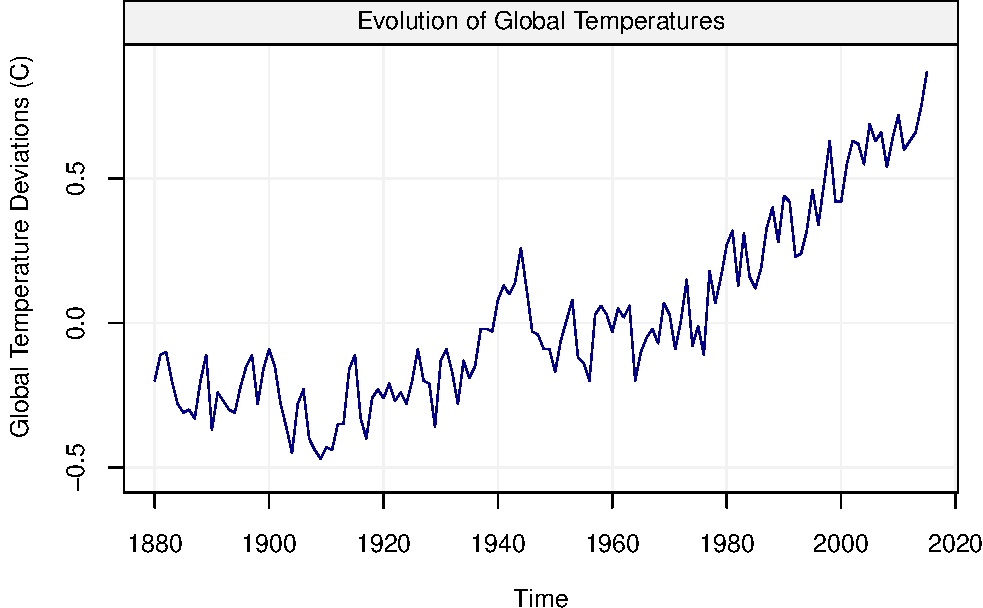
\includegraphics{ts_files/figure-latex/glotempExample-1} \end{center}

These data have been used as a support in favour of the argument that
the global temperatures are increasing and that global warming has
occured over the last half of the twentieth century. The first approach
that one would take is to try and measure the average increase by
fitting a model having the form:

\[
X_t = f(t) + \varepsilon_t,
\] where \(X_t\) denotes the global temperatures deviation and
\(f(\cdot)\) is a ``smooth'' function such that
\(\mathbb{E}[X_t] - f(t) = 0\) for all \(t\). In general,
\(\varepsilon_t\) is assumed to follow a normal distribution for
simplicity. The goal in this context would therefore be to evaluate if
\(f(t)\) (or a suitable estimator of this function) is an increasing
function (especially over the last decades). In order to do so, we would
require the residuals from the fitted model to be independently and
identically distributed (iid). Let us fit a (nonparametric) model with
the years (time) as explanatory variable using the code below:

\begin{Shaded}
\begin{Highlighting}[]
\NormalTok{time =}\StringTok{ }\KeywordTok{gts_time}\NormalTok{(globtemp)}
\NormalTok{fit =}\StringTok{ }\KeywordTok{gam}\NormalTok{(globtemp }\OperatorTok{~}\StringTok{ }\KeywordTok{s}\NormalTok{(time))}
\end{Highlighting}
\end{Shaded}

and check the residuals from this model using:

\begin{Shaded}
\begin{Highlighting}[]
\KeywordTok{check}\NormalTok{(fit, }\DataTypeTok{simple =} \OtherTok{TRUE}\NormalTok{)}
\end{Highlighting}
\end{Shaded}

\begin{verbatim}
## Warning in if (class(model) == "fitsimts") {: the condition has length > 1
## and only the first element will be used
\end{verbatim}

\begin{verbatim}
## Warning in check(fit, simple = TRUE): If 'lm' model is considered, only the
## full diagnostic plots can be provided, not the simple version.
\end{verbatim}

\begin{center}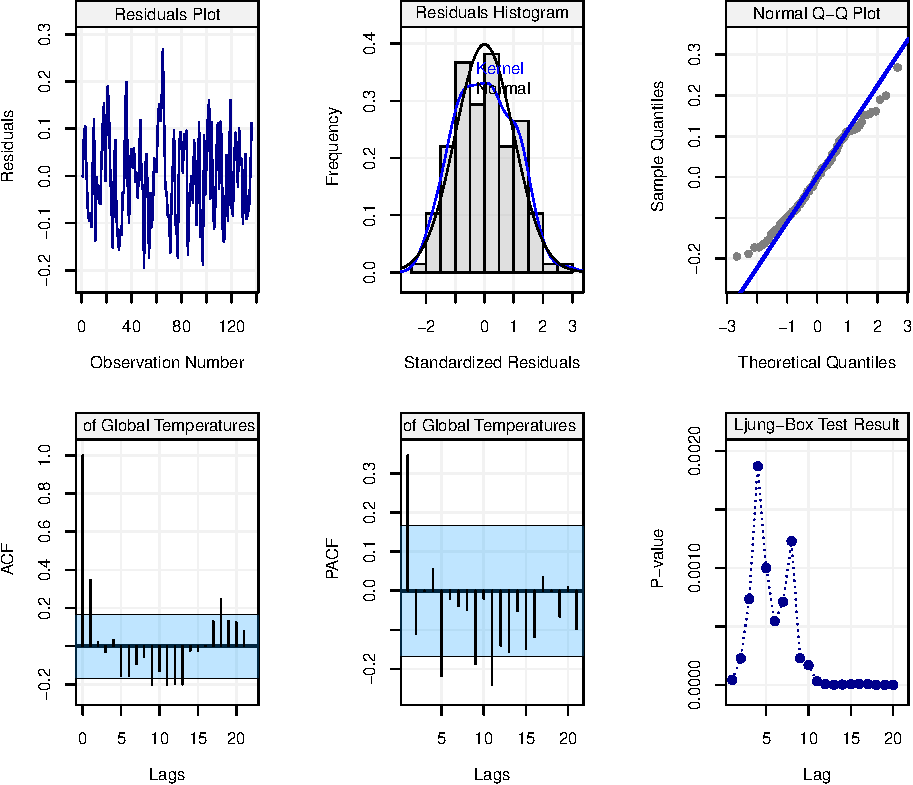
\includegraphics{ts_files/figure-latex/gamresid-1} \end{center}

It can be seen from the upper left plot that the trend appears to be
removed and, if looking at the residuals as one would usually do in a
regression framework, the residual plots seem to suggest that the
modelling has done a relatively good job since no particular pattern
seems to emerge and their distribution is quite close to being Gaussian.

However, is it possible to conclude from the plots that the data are
\emph{iid} (i.e.~independent and identically distributed)? More
specifically, can we assume that the residuals are independent? This is
a fundamental question in order for inference procedures to be carried
out in an appropriate manner and to limit false conclusions. Let us
provide an example through a simulated data set where we know that there
is an upward trend through time and our goal would be to show that this
trend exists. In order to do so we consider a simple model where
\(f(t)\) has a simple parametric form, i.e. \(f(t) = \beta \cdot t\) and
we employ the following data generating process:

\[X_t = \beta \cdot t + Y_t,\] where
\[Y_t = \phi_1 Y_{t-1} + \phi_2 Y_{t-2} + \varepsilon_t,\] and where
\(\varepsilon_t \sim \mathcal{N}(0, \sigma^2)\). Intuitively, \(Y_t\) is
not an \emph{iid} sequence of random variables except in the case where
\(\phi_1 = \phi_2 = 0\). In the following chapters we shall see that
this intuition is correct and that this model is known as an AR(2)
model. Considering this, we simulate two cases where, in the first, the
residuals are actually \emph{iid} Gaussian while, in the second, the
residuals are Gaussian but are dependent over time. In the first case,
the only parameters that explain \(X_t\) are \(\beta = 5 \cdot 10^{-3}\)
and \(\sigma^2 = 1\) since the residuals \(Y_t\) are \emph{iid} (i.e.
\(\phi_1 = \phi_2 = 0\)). In the second case however, aside from the
mentioned parameters we also have \(\phi_1 = 0.8897\),
\(\phi_2 = -0.4858\). In both cases, we perform the hypothesis test:

\[
\begin{aligned}
\text{H}_0:& \;\;\; \beta = 0\\
\text{H}_1:& \;\;\; \beta > 0
\end{aligned}
\] as our hope is to prove, similarly to the global temperature
deviation example, that \(f(t)\) is an increasing function. Our syntetic
data are simulated as follows:

\begin{Shaded}
\begin{Highlighting}[]
\CommentTok{# Set seed for reproducibility}
\KeywordTok{set.seed}\NormalTok{(}\DecValTok{9}\NormalTok{)}

\CommentTok{# Define sample size}
\NormalTok{n =}\StringTok{ }\DecValTok{100}

\CommentTok{# Define beta}
\NormalTok{beta =}\StringTok{ }\FloatTok{0.005}

\CommentTok{# Define sigma2}
\NormalTok{sigma2 =}\StringTok{ }\DecValTok{1}

\CommentTok{# Simulation of Yt}
\NormalTok{Yt_case1 =}\StringTok{ }\KeywordTok{gen_gts}\NormalTok{(}\KeywordTok{WN}\NormalTok{(}\DataTypeTok{sigma2 =}\NormalTok{ sigma2), }\DataTypeTok{n =}\NormalTok{ n)}
\NormalTok{Yt_case2 =}\StringTok{ }\KeywordTok{gen_gts}\NormalTok{(}\KeywordTok{AR}\NormalTok{(}\DataTypeTok{phi =} \KeywordTok{c}\NormalTok{(}\FloatTok{0.95}\NormalTok{, }\OperatorTok{-}\FloatTok{0.5}\NormalTok{), }\DataTypeTok{sigma2 =}\NormalTok{ sigma2), }\DataTypeTok{n =}\NormalTok{ n)}

\CommentTok{# Define explanatory variable (time)}
\NormalTok{time =}\StringTok{ }\DecValTok{1}\OperatorTok{:}\NormalTok{n}

\CommentTok{# Simulation of Xt}
\NormalTok{Xt_case1 =}\StringTok{ }\NormalTok{beta}\OperatorTok{*}\NormalTok{time }\OperatorTok{+}\StringTok{ }\NormalTok{Yt_case1}
\NormalTok{Xt_case2 =}\StringTok{ }\NormalTok{beta}\OperatorTok{*}\NormalTok{time }\OperatorTok{+}\StringTok{ }\NormalTok{Yt_case2}

\CommentTok{# Fit a linear models}
\NormalTok{model1 <-}\StringTok{ }\KeywordTok{lm}\NormalTok{(Xt_case1 }\OperatorTok{~}\StringTok{ }\NormalTok{time }\OperatorTok{+}\StringTok{ }\DecValTok{0}\NormalTok{)}
\NormalTok{model2 <-}\StringTok{ }\KeywordTok{lm}\NormalTok{(Xt_case2 }\OperatorTok{~}\StringTok{ }\NormalTok{time }\OperatorTok{+}\StringTok{ }\DecValTok{0}\NormalTok{)}
\end{Highlighting}
\end{Shaded}

The ``summary'' of our model on the first dataset is given by

\begin{Shaded}
\begin{Highlighting}[]
\KeywordTok{summary}\NormalTok{(model1)}
\end{Highlighting}
\end{Shaded}

\begin{verbatim}
## 
## Call:
## lm(formula = Xt_case1 ~ time + 0)
## 
## Residuals:
##     Min      1Q  Median      3Q     Max 
## -2.5985 -0.7023 -0.1398  0.4444  2.7098 
## 
## Coefficients:
##      Estimate Std. Error t value Pr(>|t|)  
## time 0.003930   0.001647   2.386    0.019 *
## ---
## Signif. codes:  0 '***' 0.001 '**' 0.01 '*' 0.05 '.' 0.1 ' ' 1
## 
## Residual standard error: 0.9583 on 99 degrees of freedom
## Multiple R-squared:  0.05436,    Adjusted R-squared:  0.04481 
## F-statistic: 5.691 on 1 and 99 DF,  p-value: 0.01895
\end{verbatim}

As can be seen, in the first case the estimated slope (\(\approx\)
0.004) is close to the true slope (0.005) and is significant (i.e.~the
p-value is smaller than the common rejection level 0.05) since the
p-value of the above mentioned test is given by 0.0095. Hence, from this
inference procedure we can conclude at the 5\% significance level that
the slope is significantly larger than zero and is roughly equal to
0.004 (which is relatively close to the truth). However, let us perform
the same analysis when the residuals are not independent (the second
case) by examining its ``summary'':

\begin{Shaded}
\begin{Highlighting}[]
\KeywordTok{summary}\NormalTok{(model2)}
\end{Highlighting}
\end{Shaded}

\begin{verbatim}
## 
## Call:
## lm(formula = Xt_case2 ~ time + 0)
## 
## Residuals:
##     Min      1Q  Median      3Q     Max 
## -3.6916 -1.1184  0.2323  1.1253  2.6198 
## 
## Coefficients:
##       Estimate Std. Error t value Pr(>|t|)
## time 0.0009877  0.0026435   0.374    0.709
## 
## Residual standard error: 1.538 on 99 degrees of freedom
## Multiple R-squared:  0.001408,   Adjusted R-squared:  -0.008679 
## F-statistic: 0.1396 on 1 and 99 DF,  p-value: 0.7095
\end{verbatim}

In this case we can observe that the p-value of the above mentioned test
is given by 0.3547 and is therefore greater than the arbitrary value of
0.05. Consequently, we don't have evidence to conclude that the slope
coefficient is larger than zero (i.e.~we fail to reject H\(_0\))
although it is actually so in reality. Therefore, the inference
procedures can be misleading when not taking into account other possible
significant variables or, in this case, forms of dependence that can
hide true underlying effects. The above is only one example and there
are therefore cases where, despite dependence in the residuals, the
estimated slope would be deemed significant even when not considering
this dependence structure. However, if we decided to repeat this
experiment using a larger quantity of simulated samples, we would
probably see that we fail to reject the null hypothesis much more
frequently in the case where we don't consider dependence when there
actually is.

These examples therefore highlight how the approach to analysing time
series does not only rely on finding an appropriate model that describes
the evolution of a variable as a function of time (which is
deterministic). Indeed, one of the main focuses of time series analysis
consists in modelling the dependence structure that describes how random
variables impact each other as a function of time. In other words, a
time series is a collection of random variables whose interaction and
dependence structure is indexed by time. Based on this structure, one of
the main goals of time series analysis is to correctly estimate the
dependence mechanism and consequently deliver forecasts that are as
accurate as possible considering the deterministic functions of time
(and other variables) as well as the random dependence structure.

\section{The Wold Decomposition}\label{the-wold-decomposition}

The previous discussion highlighted how a time series can be decomposed
into a deterministic component and a random component. Leaving aside
technical rigour, this characteristic of time series was put forward in
Wold's Decomposition Theorem who postulated that a time series \((Y_t)\)
(where \(t = 1,...,n\) represents the time index) can be very
generically represented as follows:

\[Y_t = D_t + W_t,\]

where \(D_t\) represents the deterministic part (or \emph{signal}) that
can be modelled through the standard modelling techniques (e.g.~linear
regression) and \(W_t\) that, restricting ourselves to a general class
of processes, represents the random part (\emph{noise}) that requires
the analytical and modelling approaches that will be tackled in this
book.

Typically, we have \(\mathbb{E}[Y_t] \neq 0\) while
\(\mathbb{E}[W_t] = 0\) (although we may have
\(\mathbb{E}[W_t | W_{t-1}, ..., W_1] \neq 0\)). Such models impose some
parametric structure which represents a convenient and flexible way of
studying time series as well as a means to evaluate \emph{future} values
of the series through forecasting. As we will see, predicting future
values is one of the main aspects of time series analysis. However,
making predictions is often a daunting task or as famously stated by
Nils Bohr:

\begin{quote}
``\emph{Prediction is very difficult, especially about the future.}''
\end{quote}

There are plenty of examples of predictions that turned out to be
completely erroneous. For example, three days before the 1929 crash,
Irving Fisher, Professor of Economics at Yale University, famously
predicted:

\begin{quote}
``\emph{Stock prices have reached what looks like a permanently high
plateau}''.
\end{quote}

Another example is given by Thomas Watson, president of IBM, who said in
1943:

\begin{quote}
``\emph{I think there is a world market for maybe five computers.}''
\end{quote}

Let us now briefly discuss the two components of a time series.

\subsection{The Deterministic Component
(Signal)}\label{the-deterministic-component-signal}

Before shifting our focus to the random component of time series, we
will first just underline the main features that should be taken into
account for the deterministic component. The first feature that should
be analysed is the \emph{trend} that characterises the time series, more
specifically the behaviour of the variable of interest as a specific
function of time (as the global temperature time series seen earlier).
Let us consider another example borrowed from \citet{shumway2010time} of
time series based on real data, i.e.~the quarterly earnings of Johnson
\& Johnson between 1960 and 1980 represented below.

\begin{Shaded}
\begin{Highlighting}[]
\CommentTok{# Load data}
\KeywordTok{data}\NormalTok{(jj, }\DataTypeTok{package =} \StringTok{"astsa"}\NormalTok{)}

\CommentTok{# Construct gts object}
\NormalTok{jj =}\StringTok{ }\KeywordTok{gts}\NormalTok{(jj, }\DataTypeTok{start =} \DecValTok{1960}\NormalTok{, }\DataTypeTok{freq =} \DecValTok{4}\NormalTok{, }\DataTypeTok{unit_ts =} \StringTok{"$"}\NormalTok{, }\DataTypeTok{name_ts =} \StringTok{"Quarterly Earnings per Share"}\NormalTok{, }\DataTypeTok{data_name =} \StringTok{"Johnson & Johnson Quarterly Earnings"}\NormalTok{)}

\CommentTok{# Plot time series}
\KeywordTok{plot}\NormalTok{(jj)}
\end{Highlighting}
\end{Shaded}

\begin{center}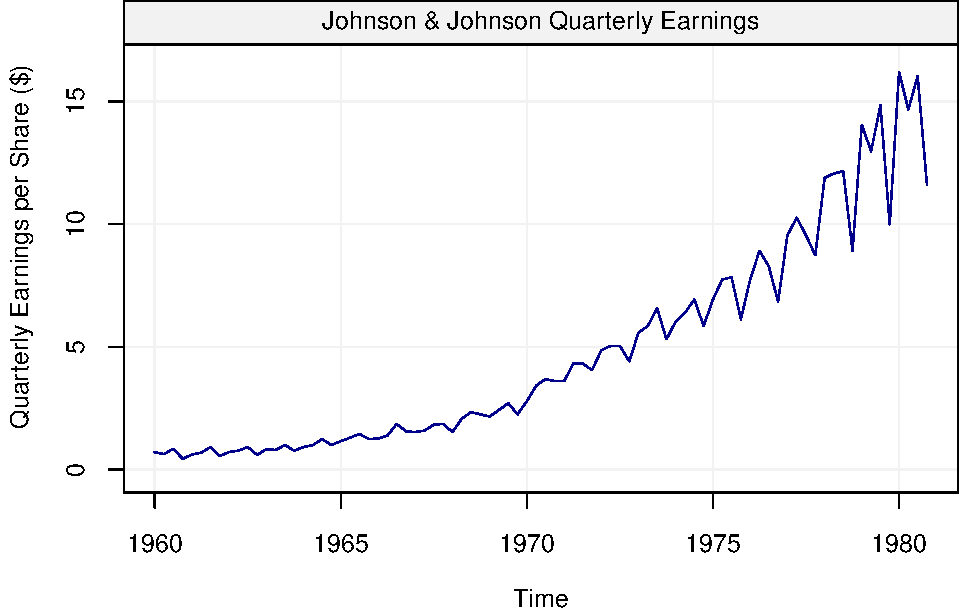
\includegraphics{ts_files/figure-latex/jjexample-1} \end{center}

As can be seen from the plot, the earnings appear to grow over time,
therefore we can imagine fitting a straight line to this data to
describe its behaviour by considering the following model:

\begin{equation} 
X_t = \alpha + \beta t + \varepsilon_t,
\label{eq:modeljjexample}
\end{equation}

where \(\varepsilon_t\) is iid Gaussian. The results are presented in
the graph below:

\begin{Shaded}
\begin{Highlighting}[]
\CommentTok{# Fit linear regression}
\NormalTok{time_jj =}\StringTok{ }\KeywordTok{gts_time}\NormalTok{(jj)}
\NormalTok{fit_jj1 =}\StringTok{ }\KeywordTok{lm}\NormalTok{(}\KeywordTok{as.vector}\NormalTok{(jj) }\OperatorTok{~}\StringTok{ }\NormalTok{time_jj)}

\CommentTok{# Plot results and add regression line}
\KeywordTok{plot}\NormalTok{(jj)}
\KeywordTok{lines}\NormalTok{(time_jj, }\KeywordTok{predict}\NormalTok{(fit_jj1), }\DataTypeTok{col =} \StringTok{"red"}\NormalTok{)}
\KeywordTok{legend}\NormalTok{(}\StringTok{"bottomright"}\NormalTok{, }\KeywordTok{c}\NormalTok{(}\StringTok{"Time series"}\NormalTok{, }\StringTok{"Regression line"}\NormalTok{), }
       \DataTypeTok{col =} \KeywordTok{c}\NormalTok{(}\StringTok{"blue4"}\NormalTok{, }\StringTok{"red"}\NormalTok{), }\DataTypeTok{bty =} \StringTok{"n"}\NormalTok{, }\DataTypeTok{lwd =} \DecValTok{1}\NormalTok{)}
\end{Highlighting}
\end{Shaded}

\begin{center}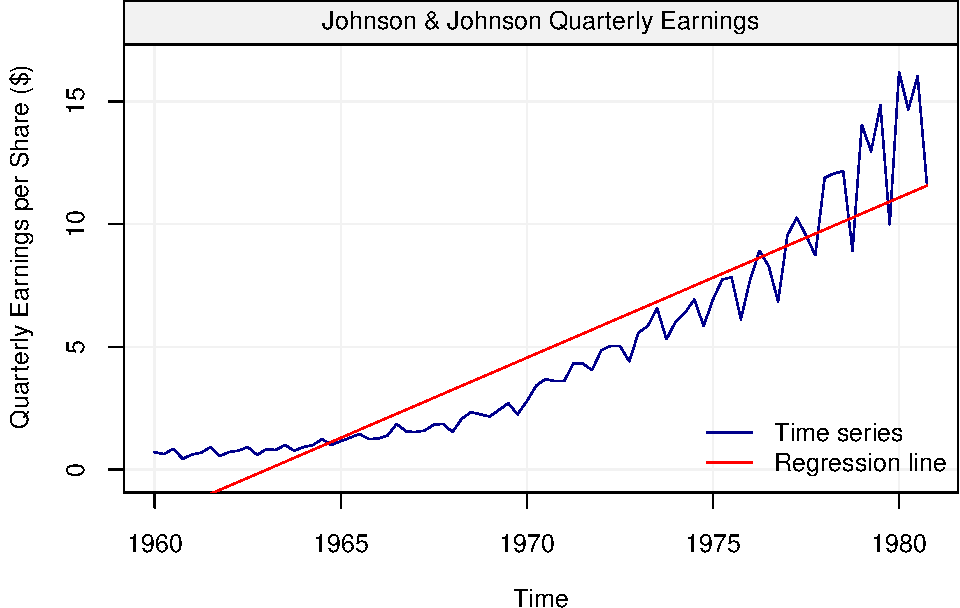
\includegraphics{ts_files/figure-latex/jjexample2-1} \end{center}

Although the line captures a part of the behaviour, it is quite clear
that the trend of the time series is not linear as can be observed from
the diagnotic plot below:

\begin{Shaded}
\begin{Highlighting}[]
\KeywordTok{check}\NormalTok{(fit_jj1, }\DataTypeTok{simple =} \OtherTok{TRUE}\NormalTok{)}
\end{Highlighting}
\end{Shaded}

\begin{verbatim}
## Warning in check(fit_jj1, simple = TRUE): If 'lm' model is considered, only
## the full diagnostic plots can be provided, not the simple version.
\end{verbatim}

\begin{center}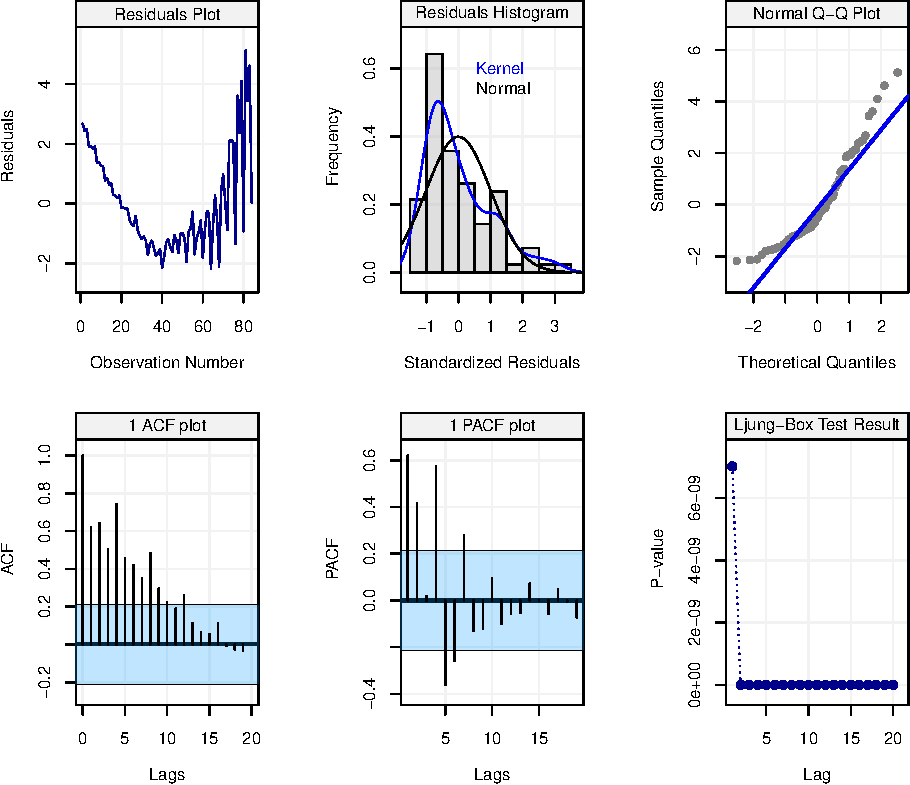
\includegraphics{ts_files/figure-latex/lmresid-1} \end{center}

It could therefore be more appropriate to define another function of
time to describe it and, consequently, we add a quadratic term of time
to obtain the following fit. Therefore, the model considered in
\eqref{eq:modeljjexample} becomes:

\begin{equation} 
X_t = \alpha + \beta_1 t + \beta_2 t^2 + \varepsilon_t,
\label{eq:modeljjexample2}
\end{equation}

The results of this regression are presented on the graphs below:

\begin{center}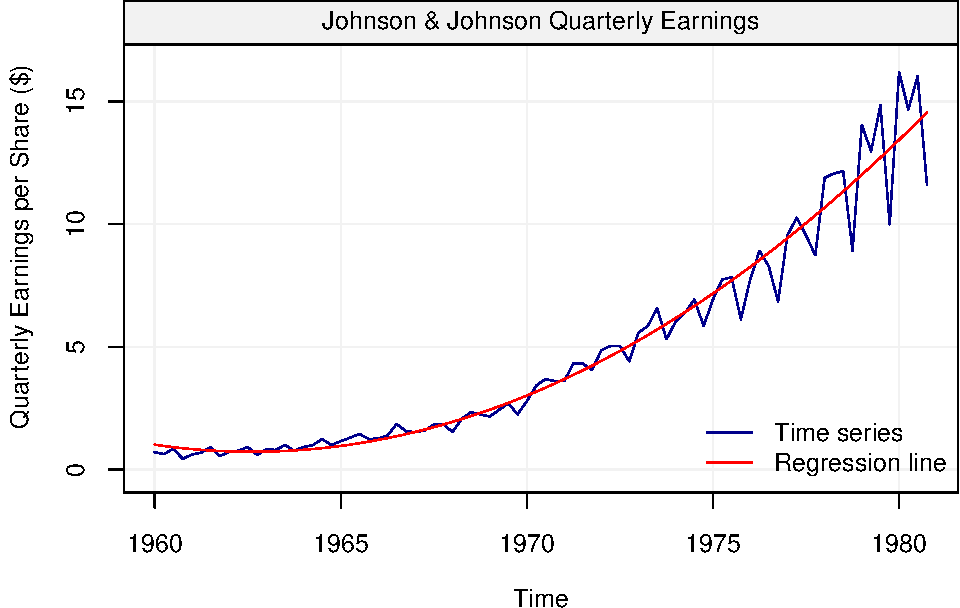
\includegraphics{ts_files/figure-latex/unnamed-chunk-16-1} \end{center}

\begin{Shaded}
\begin{Highlighting}[]
\KeywordTok{check}\NormalTok{(fit_jj2, }\DataTypeTok{simple =} \OtherTok{TRUE}\NormalTok{)}
\end{Highlighting}
\end{Shaded}

\begin{verbatim}
## Warning in check(fit_jj2, simple = TRUE): If 'lm' model is considered, only
## the full diagnostic plots can be provided, not the simple version.
\end{verbatim}

\begin{center}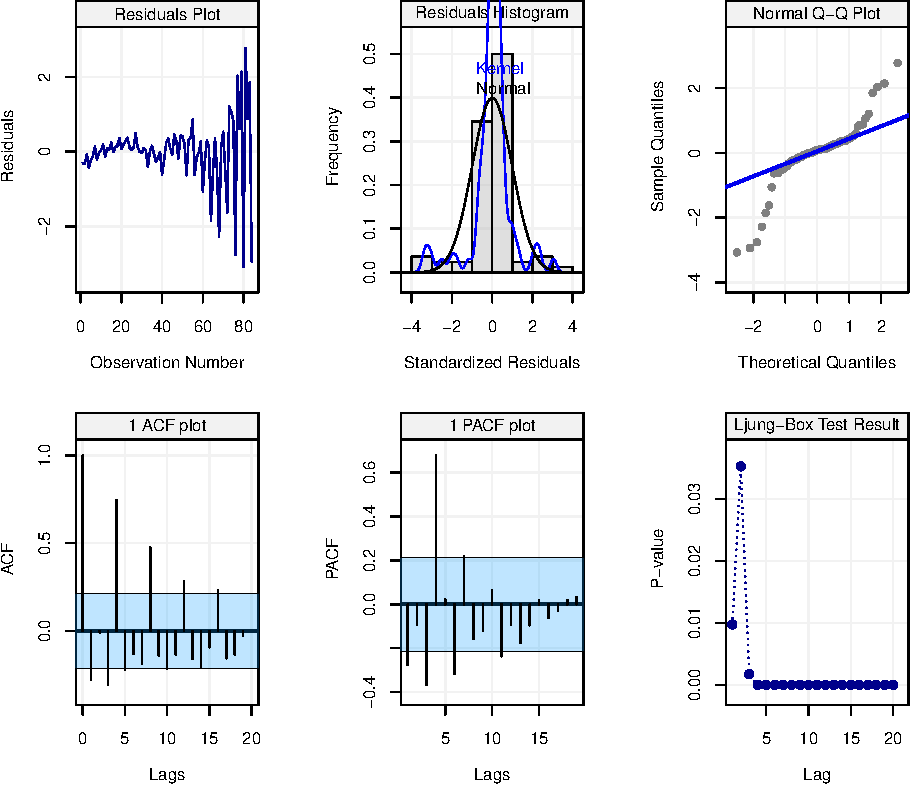
\includegraphics{ts_files/figure-latex/lmresid2-1} \end{center}

We can see now that the quadratic function of time allows to better fit
the observed time series and closely follow the observations. However,
there still appears to be a pattern in the data that isn't captured by
this quadratic model. This pattern appears to be repeated over time:
peaks and valleys that seem to occur at regular intervals along the time
series. This behaviour is known as \emph{seasonality} which, in this
case, can be explained by the effect of a specific quarter on the
behaviour of the earnings. Indeed, it is reasonable to assume that the
seasons have impacts on different variables measured over time
(e.g.~temperatures, earnings linked to sales that vary with seasons,
etc.). Let us therefore take the quarters as an explanatory variable and
add it to the model considered in \eqref{eq:modeljjexample2}, which
becomes:

\begin{equation} 
X_t = \alpha + \beta_1 t + \beta_2 t^2 + \sum_{i = 1}^4 \gamma_i I_{t \in \mathcal{A}_i} + \varepsilon_t,
\label{eq:modeljjexample3}
\end{equation}

where

\begin{equation*}
  I_{t \in \mathcal{A}} \equiv \left\{
    \begin{array}{ll}
        1  & \mbox{if } t \in \mathcal{A} \\
        0 & \mbox{if } t \not\in \mathcal{A}
    \end{array}
\right. ,
\end{equation*}

and where

\[
\mathcal{A}_i \equiv \left\{x \in \mathbb{N} | x = i \; \text{mod} \;  4\right\}.
\]

The results are presented below:

\begin{center}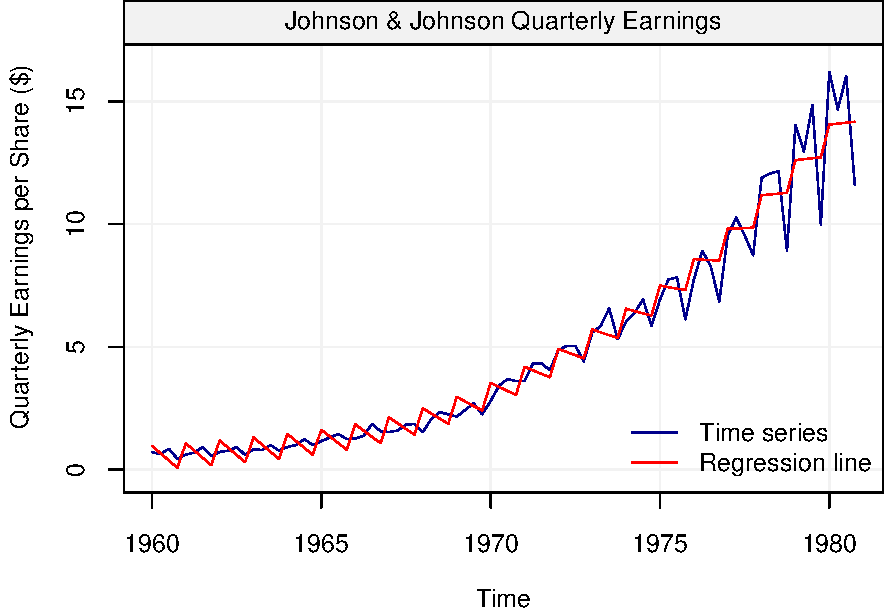
\includegraphics{ts_files/figure-latex/unnamed-chunk-17-1} \end{center}

\begin{Shaded}
\begin{Highlighting}[]
\KeywordTok{check}\NormalTok{(fit_jj3, }\DataTypeTok{simple =} \OtherTok{TRUE}\NormalTok{)}
\end{Highlighting}
\end{Shaded}

\begin{verbatim}
## Warning in if (class(model) == "fitsimts") {: the condition has length > 1
## and only the first element will be used
\end{verbatim}

\begin{verbatim}
## Warning in check(fit_jj3, simple = TRUE): If 'lm' model is considered, only
## the full diagnostic plots can be provided, not the simple version.
\end{verbatim}

\begin{center}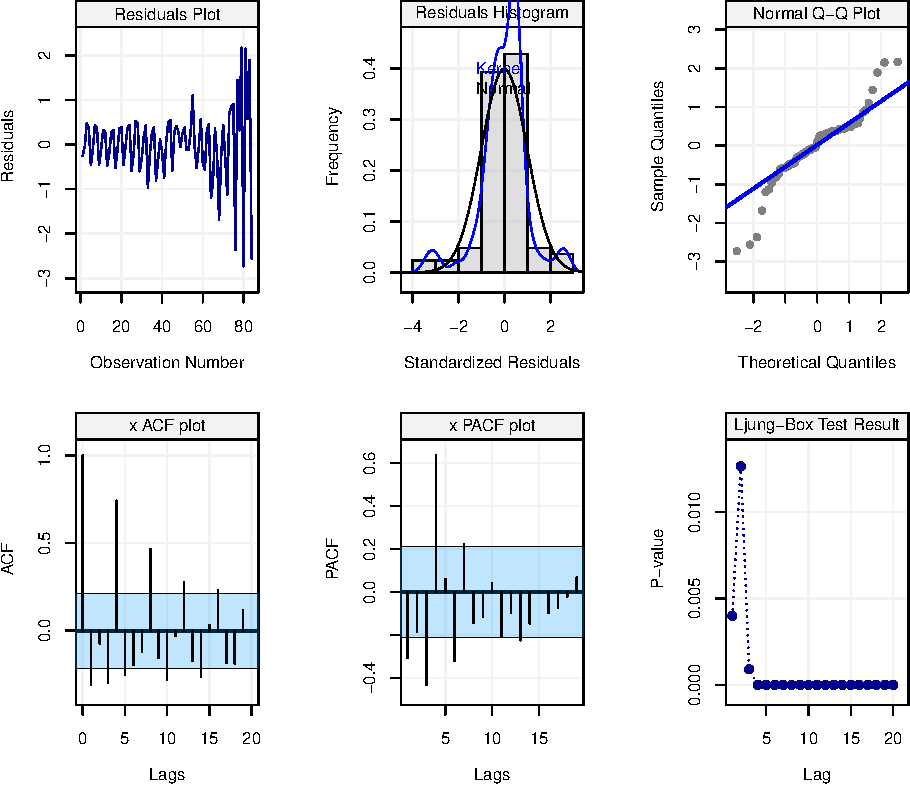
\includegraphics{ts_files/figure-latex/lmresid3-1} \end{center}

This final fit appears to well describe the behaviour of the earnings
although there still appears to be a problem of heteroskedasticity
(i.e.~change in variance) and random seasonality (both of which will be
treated further on in this text). Hence, \emph{trend} and
\emph{seasonality} are the main features that characterize the
deterministic component of a time series. However, as discussed earlier,
these deterministic components often don't explain all of the observed
time series since there is often a random component characterizing data
measured over time. Not considering the latter component can have
considerable impacts on the inference procedures (as seen earlier) and
it is therefore important to adequately analyse them (see next section).

\subsection{The Random Component
(Noise)}\label{the-random-component-noise}

From this section onwards we will refer to \emph{time series as being
solely the random noise component}. Keeping this in mind, a \emph{time
series} is a particular kind of \emph{stochastic process} which,
generally speaking, is a collection of random variables indexed by a set
of numbers. Not surprisingly, the index of reference for a time series
is given by \emph{time} and, consequently, a time series is a collection
of random variables indexed (or ``measured'') over time such as, for
example, the daily price of a financial asset or the monthly average
temperature in a given location. In terms of notation, a time series is
often represented as

\[\left(X_1, X_2, ..., X_T \right) \;\;\; \text{ or } \;\;\; \left(X_t\right)_{t = 1,...,T}.\]

The time index \(t\) is contained within either the set of reals,
\(\mathbb{R}\), or integers, \(\mathbb{Z}\). When \(t \in \mathbb{R}\),
the time series becomes a \emph{continuous-time} stochastic process such
as a Brownian motion, a model used to represent the random movement of
particles within a suspended liquid or gas. However, within this book,
we will limit ourselves to the cases where \(t \in \mathbb{Z}\), better
known as \emph{discrete-time} processes. Discrete-time processes are
measured sequentially at fixed and equally spaced intervals in time.
This implies that we will uphold two general assumptions for the time
series considered in this book:

\begin{enumerate}
\def\labelenumi{\arabic{enumi}.}
\tightlist
\item
  \(t\) is not random, e.g.~the time at which each observation is
  measured is known, and
\item
  the time between two consecutive observations is constant.
\end{enumerate}

This book will also focus on certain representations of time series
based on parametric probabilistic models. For example, one of the
fundamental probability models used in time series analysis is called
the \emph{white noise} model and is defined as

\[X_t \mathop \sim \limits^{iid} N(0, \sigma^2).\]

This statement simply means that \((X_t)\) is normally distributed and
independent over time. Ideally, this is the type of process that we
would want to observe once we have performed a statistical modelling
procedure. However, despite it appearing to be an excessively simple
model to be considered for time series, it is actually a crucial
component to construct a wide range of more complex time series models
(see Chapter \ref{fundtimeseries}). Indeed, unlike the white noise
process, time series are typically \emph{not} independent over time. For
example, if we suppose that the temperature in State College is
unusually low on a given day, then it is reasonable to assume that the
temperature the day after will also be low.

With this in mind, let us now give a quick overview of the information
that can be retrieved on a time series from a simple descriptive
representation.

\section{Exploratory Data Analysis for Time Series}\label{eda}

When dealing with relatively small time series (e.g.~a few thousands or
less), it is often useful to look at a graph of the original data. A
graph can be an informative tool for ``detecting'' some features of a
time series such as trends and the presence of outliers. This is indeed
what was done in the previous paragraphs when analysing the global
temperature data or the Johnson \& Johnson data.

To go more in depth with respect to the previous paragraphs, a trend is
typically assumed to be present in a time series when the data exhibit
some form of long term increase or decrease or combination of increases
or decreases. Such trends could be linear or non-linear and represent an
important part of the ``signal'' of a model (as seen for the Johnson \&
Johnson time series). Here are a few examples of non-linear trends:

\begin{enumerate}
\def\labelenumi{\arabic{enumi}.}
\item
  \textbf{Seasonal trends} (periodic): These are the cyclical patterns
  which repeat after a fixed/regular time period. This could be due to
  business cycles (e.g.~bust/recession, recovery).
\item
  \textbf{Non-seasonal trends} (periodic): These patterns cannot be
  associated to seasonal variation and can for example be due to an
  external variable such as, for example, the impact of economic
  indicators on stock returns. Note that such trends are often hard to
  detect based on a graphical analysis of the data.
\item
  \textbf{``Other'' trends}: These trends have typically no regular
  patterns and are over a segment of time, known as a ``window'', that
  change the statistical properties of a time series. A common example
  of such trends is given by the vibrations observed before, during and
  after an earthquake.
\end{enumerate}

Moreover, when observing ``raw'' time series data it is also interesting
to evaluate if some of the following phenomena occur:

\begin{enumerate}
\def\labelenumi{\arabic{enumi}.}
\tightlist
\item
  \textbf{Change in Mean:} Does the mean of the process shift over time?
\item
  \textbf{Change in Variance:} Does the variance of the process evolve
  with time?
\item
  \textbf{Change in State:} Does the time series appear to change
  between ``states'' having distinct statistical properties?
\item
  \textbf{Outliers} Does the time series contain some ``extreme''
  observations? (Note that this is typically difficult to assess
  visually.)
\end{enumerate}

\BeginKnitrBlock{example}
\protect\hypertarget{exm:earthquake}{}{\label{exm:earthquake} }In the figure
below, we present an example of displacement recorded during an
earthquake as well as an explosion.
\EndKnitrBlock{example}

\begin{Shaded}
\begin{Highlighting}[]
\KeywordTok{data}\NormalTok{(EQ5, }\DataTypeTok{package =} \StringTok{"astsa"}\NormalTok{)}
\KeywordTok{data}\NormalTok{(EXP6, }\DataTypeTok{package =} \StringTok{"astsa"}\NormalTok{)}

\CommentTok{# Construct gts object}
\NormalTok{eq5 <-}\StringTok{ }\KeywordTok{gts}\NormalTok{(EQ5, }\DataTypeTok{start =} \DecValTok{0}\NormalTok{, }\DataTypeTok{freq =} \DecValTok{1}\NormalTok{, }\DataTypeTok{unit_ts =} \StringTok{"p/s"}\NormalTok{, }\DataTypeTok{name_ts =} \StringTok{"Earthquake Arrival Phases"}\NormalTok{, }\DataTypeTok{data_name =} \StringTok{"Earthquake Arrival Phases"}\NormalTok{)}
\NormalTok{exp6 <-}\StringTok{ }\KeywordTok{gts}\NormalTok{(EXP6, }\DataTypeTok{start =} \DecValTok{0}\NormalTok{, }\DataTypeTok{freq =} \DecValTok{1}\NormalTok{, }\DataTypeTok{unit_ts =} \StringTok{"p/s"}\NormalTok{, }\DataTypeTok{name_ts =} \StringTok{"Explosion Arrival Phases"}\NormalTok{, }\DataTypeTok{data_name =} \StringTok{"Explosion Arrival Phases"}\NormalTok{)}

\CommentTok{# Plot time series}
\KeywordTok{plot}\NormalTok{(eq5)}
\end{Highlighting}
\end{Shaded}

\begin{center}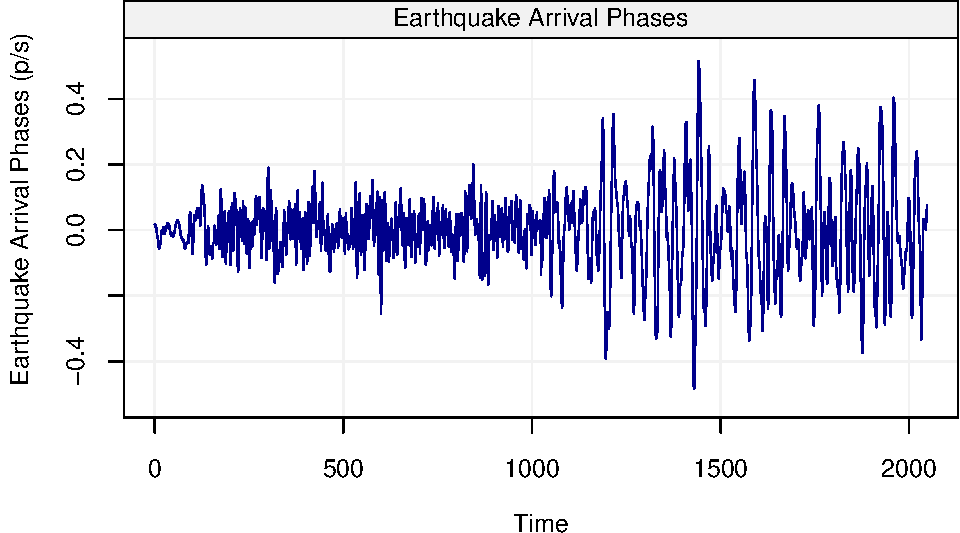
\includegraphics{ts_files/figure-latex/example_EQ-1} \end{center}

\begin{Shaded}
\begin{Highlighting}[]
\KeywordTok{plot}\NormalTok{(exp6)}
\end{Highlighting}
\end{Shaded}

\begin{center}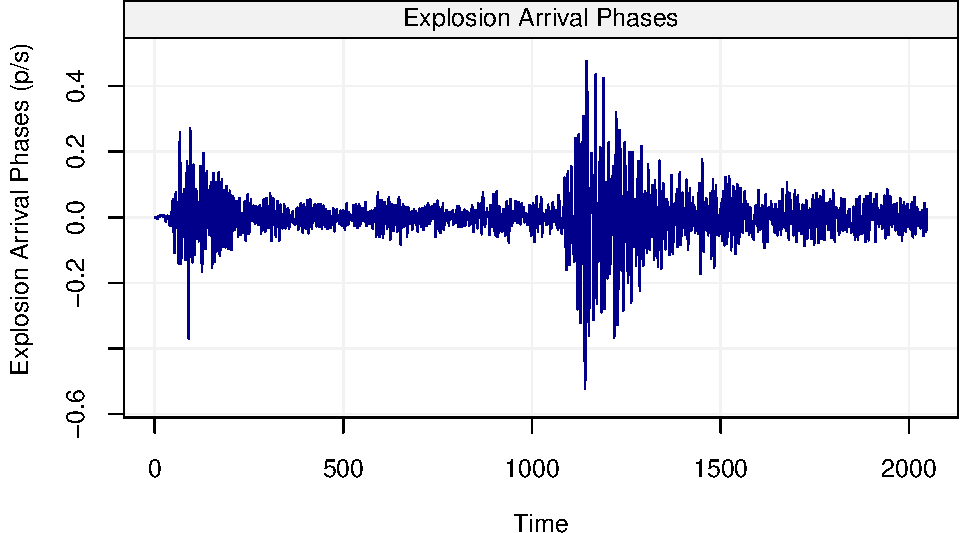
\includegraphics{ts_files/figure-latex/example_EQ-2} \end{center}

From the graph, it can be observed that the statistical properties of
the time series appear to change over time. For instance, the variance
of the time series shifts at around \(t = 1150\) for both series. The
shift in variance also opens ``windows'' where there appear to be
distinct states. In the case of the explosion data, this is particularly
relevant around \(t = 50, \cdots, 250\) and then again from
\(t = 1200, \cdots, 1500\). Even within these windows, there are
``spikes'' that could be considered as outliers most notably around
\(t = 1200\) in the explosion series.

Extreme observations or outliers are commonly observed in real time
series data, this is illustrated in the following example.

\BeginKnitrBlock{example}
\protect\hypertarget{exm:precipitation}{}{\label{exm:precipitation} }We
consider here a data set coming from the domain of hydrology. The data
concerns monthly precipitation (in mm) over a certain period of time
(1907 to 1972) and is interesting for scientists in order to study water
cycles. The data are presented in the graph below:
\EndKnitrBlock{example}

\begin{Shaded}
\begin{Highlighting}[]
\CommentTok{# Load hydro dataset}
\KeywordTok{data}\NormalTok{(}\StringTok{"hydro"}\NormalTok{)}

\CommentTok{# Simulate based on data}
\NormalTok{hydro =}\StringTok{ }\KeywordTok{gts}\NormalTok{(}\KeywordTok{as.vector}\NormalTok{(hydro), }\DataTypeTok{start =} \DecValTok{1907}\NormalTok{, }\DataTypeTok{freq =} \DecValTok{12}\NormalTok{, }\DataTypeTok{unit_ts =} \StringTok{"in."}\NormalTok{, }
            \DataTypeTok{name_ts =} \StringTok{"Precipitation"}\NormalTok{, }\DataTypeTok{data_name =} \StringTok{"Hydrology data"}\NormalTok{)}

\CommentTok{# Plot hydro }
\KeywordTok{plot}\NormalTok{(hydro)}
\end{Highlighting}
\end{Shaded}

\begin{center}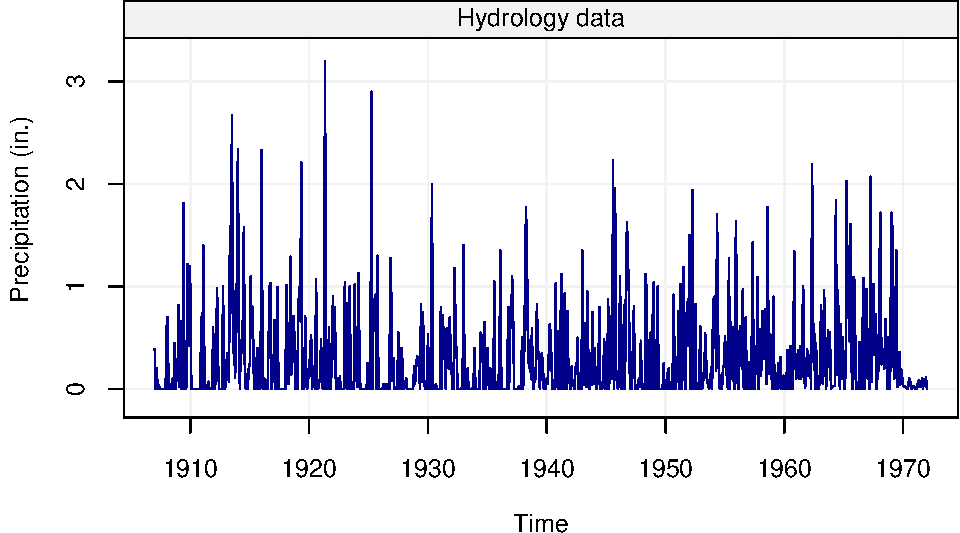
\includegraphics{ts_files/figure-latex/example_hydro-1} \end{center}

We can see how most observations lie below 2mm but there appear to be
different observations that go beyond this and appear to be larger than
the others. These could be possible outliers that can greatly affect the
estimation procedure if not taken adequately into account.

Next, we consider an example coming from high-frequency finance. The
figure below presents the returns or price innovations (i.e.~the changes
in price from one observation to the next) for Starbuck's stock on July
1, 2011 for about 150 seconds (left panel) and about 400 minutes (right
panel).

\begin{Shaded}
\begin{Highlighting}[]
\CommentTok{# Load "high-frequency" Starbucks returns for July 01 2011}
\KeywordTok{data}\NormalTok{(sbux.xts, }\DataTypeTok{package =} \StringTok{"highfrequency"}\NormalTok{)}

\CommentTok{# Plot returns}
\KeywordTok{par}\NormalTok{(}\DataTypeTok{mfrow =} \KeywordTok{c}\NormalTok{(}\DecValTok{1}\NormalTok{,}\DecValTok{2}\NormalTok{))}

\KeywordTok{plot}\NormalTok{(}\KeywordTok{gts}\NormalTok{(sbux.xts[}\DecValTok{1}\OperatorTok{:}\DecValTok{89}\NormalTok{]), }
     \DataTypeTok{main =} \StringTok{"Starbucks: 150 Seconds"}\NormalTok{, }
     \DataTypeTok{ylab =} \StringTok{"Returns"}\NormalTok{) }

\KeywordTok{plot}\NormalTok{(}\KeywordTok{gts}\NormalTok{(sbux.xts), }
     \DataTypeTok{main =} \StringTok{"Starbucks: 400 Minutes"}\NormalTok{, }
     \DataTypeTok{ylab =} \StringTok{"Returns"}\NormalTok{)}
\end{Highlighting}
\end{Shaded}

\begin{center}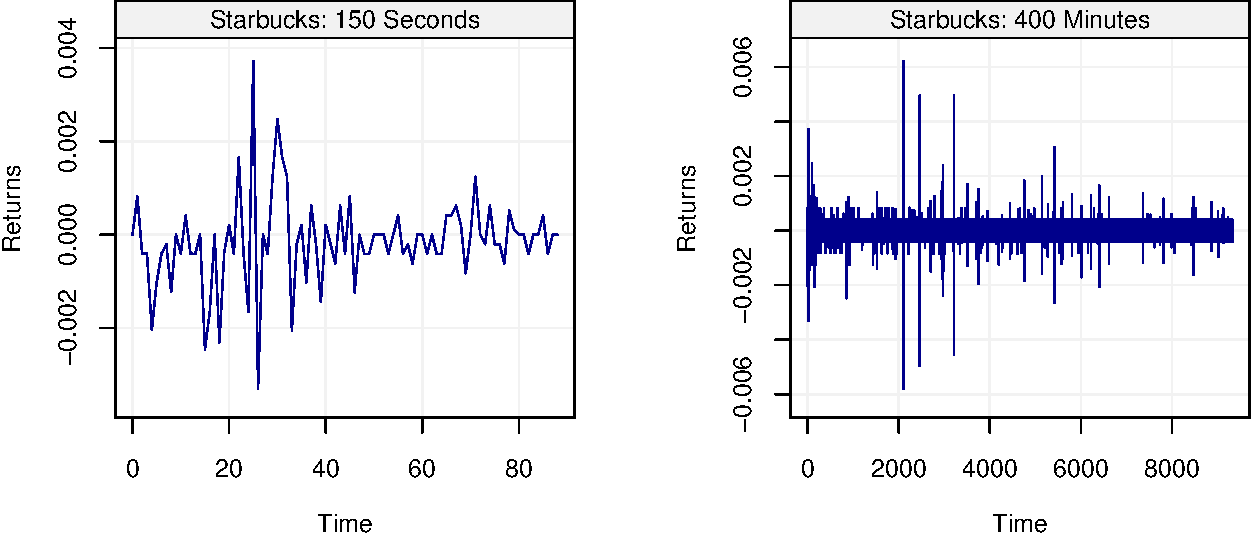
\includegraphics{ts_files/figure-latex/example_Starbucks-1} \end{center}

It can be observed on the left panel that observations are not equally
spaced. Indeed, in high-frequency data the intervals between two points
are typically not constant and are, even worse, random variables. This
implies that the time when a new observation will be available is in
general unknown. On the right panel, one can observe that the
variability of the data seems to change during the course of the trading
day. Such a phenomenon is well known in the finance community since a
lot of variation occurs at the start (and the end) of the day while the
middle of the day is associated with small changes. Moreover, clear
extreme observations can also be noted in this graph at around 11:00.

\BeginKnitrBlock{example}
\protect\hypertarget{exm:imu}{}{\label{exm:imu} }Finally, let us consider
the limitations of a direct graphical representation of a time series
when the sample size is large. Indeed, due to visual limitations, a
direct plotting of the data will probably result in an uninformative
aggregation of points between which it is unable to distinguish
anything. This is illustrated in the following example.

We consider here the data coming from the calibration procedure of an
Inertial Measurement Unit (IMU) which, in general terms, is used to
enhance navigation precision or reconstruct three dimensional movements:
\EndKnitrBlock{example}

These sensors are used in a very wide range of applications such as
robotics, virtual reality 🐻, vehicle stability control, human and animal
motion capture and so forth:

The signals coming from these instruments are measured at high
frequencies over a long time and are often characterized by linear
trends and numerous underlying stochastic processes.

The code below retrieves some data from an IMU and plots it directly:

\BeginKnitrBlock{rmdimportant}
To access the IMU time series represented below you must install the
imudata package which can be found at this
\href{https://github.com/SMAC-Group/imudata}{link}.
\EndKnitrBlock{rmdimportant}

\begin{Shaded}
\begin{Highlighting}[]
\CommentTok{# Load IMU data}
\KeywordTok{data}\NormalTok{(imu6, }\DataTypeTok{package =} \StringTok{"imudata"}\NormalTok{)}

\CommentTok{# Construct gst object}
\NormalTok{Xt =}\StringTok{ }\KeywordTok{gts}\NormalTok{(imu6[,}\DecValTok{1}\NormalTok{], }\DataTypeTok{data_name =} \StringTok{"Gyroscope data"}\NormalTok{, }\DataTypeTok{unit_time =} \StringTok{"hour"}\NormalTok{, }
         \DataTypeTok{freq =} \DecValTok{100}\OperatorTok{*}\DecValTok{60}\OperatorTok{*}\DecValTok{60}\NormalTok{, }\DataTypeTok{name_ts =} \StringTok{"Angular rate"}\NormalTok{, }
         \DataTypeTok{unit_ts =} \KeywordTok{bquote}\NormalTok{(rad}\OperatorTok{^}\DecValTok{2}\OperatorTok{/}\NormalTok{s}\OperatorTok{^}\DecValTok{2}\NormalTok{))}

\CommentTok{# Plot time series}
\KeywordTok{plot}\NormalTok{(Xt)}
\end{Highlighting}
\end{Shaded}

\begin{center}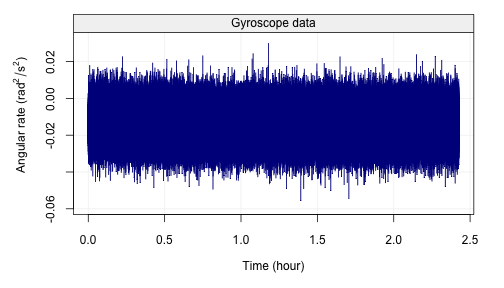
\includegraphics{ts_files/figure-latex/example_IMU-1} \end{center}

Although a linear trend and other processes are present in this signal
(time series), it is practically impossible to understand or guess
anything from the plot. For this reason, other types of representations
are available to understand the behaviour of a time series and will be
discussed in the next chapter. Having discussed these representations
(and the relative issues with these representations) let us present the
basic parametric models that are used to build even more complex models
to describe and predict the behaviour of a time series.

\section{Dependence in Time Series}\label{dependence-in-time-series}

In this seciton we briefly discuss the concept of dependence (within
time series). As mentioned earlier, it is straightforward to assume that
observations measured through time are dependent on each other (in that
observations at time \(t\) have some form of impact on observations at
time \(t+1\) or beyond). Due to this characteristic, one of the main
interests in time series is prediction where, if
\((X_t)_{t=1,\ldots,T}\) is an identically distributed but not
independent sequence, we often want to know the value of \({X}_{T+h}\)
for \(h > 0\) (i.e.~an estimator of \(\mathbb{E}[X_{T+h}| X_T,...]\)).
In order to tackle this issue, we first need to understand the
dependence between \(X_{1},\ldots,X_{T}\) and, even before this, we have
to formally define what \textbf{independence} is.

\BeginKnitrBlock{definition}[Independence of Events]
\protect\hypertarget{def:IndepEvents}{}{\label{def:IndepEvents}
\iffalse (Independence of Events) \fi{} }Two events \(A\) and \(B\) are
independent if

\begin{align*}
\mathbb{P}(A \cap B) = \mathbb{P}(A)\mathbb{P}(B),
\end{align*}

with \(\mathbb{P}(A)\) denoting the probability of event \(A\) occuring
and \(\mathbb{P}(A \cap B)\) denoting the joint probability (i.e.~the
probability that events \(A\) and \(B\) occur jointly). In general,
\(A_{1},\ldots,A_{n}\) are independent if

\begin{align*}
\mathbb{P}(A_1 \ldots A_n) = \mathbb{P}(A_1) \ldots \mathbb{P}(A_n) \;\; \forall \; A_i \in S, \;\; i=1,\ldots,n
\end{align*}

where \(S\) is the sample space.
\EndKnitrBlock{definition}

\BeginKnitrBlock{definition}[Independence of Random Variables]
\protect\hypertarget{def:IndepRV}{}{\label{def:IndepRV}
\iffalse (Independence of Random Variables) \fi{} }Two random variables
\(X\) and \(Y\) with Cumulative Distribution Functions (CDF) \(F_X(x)\)
and \(F_Y(y)\), respectively, are independent if and only if their joint
CDF \(F_{X,Y}(x,y)\) is such that

\begin{align*}
F_{X,Y}(x,y) = F_{X}(x) F_{Y}(y).
\end{align*}

In general, random variables \(X_1, \ldots, X_n\) with CDF
\(F_{X_1}(x_1), \ldots, F_{X_n}(x_n)\) are respectively independent if
and only if their joint CDF \(F_{X_1, \ldots, X_n}(x_1, \ldots, x_n)\)
is such that

\begin{align*}
F_{X_1,\ldots,X_n}(x_1,\ldots,x_n) = F_{X_1}(x_1) \ldots F_{X_n}(x_n).
\end{align*}
\EndKnitrBlock{definition}

\BeginKnitrBlock{definition}[iid sequence]
\protect\hypertarget{def:iid}{}{\label{def:iid} \iffalse (iid sequence)
\fi{} }The sequence \(X_{1},X_{2},\ldots,X_{T}\) is said to be
independent and identically distributed (i.e.~iid) if and only if

\begin{align*}
\mathbb{P}(X_{i}<x) = \mathbb{P}(X_{j}<x) \;\; \forall x \in \mathbb{R}, \forall i,j \in \{1,\ldots,T\},
\end{align*}

and

\begin{align*}
\mathbb{P}(X_{1}<x_{1},X_{2}<x_{2},\ldots,X_{T}<x_{T})=\mathbb{P}(X_{1}<x_1) \ldots \mathbb{P}(X_{T}<x_T) \;\; \forall T\geq2, x_1, \ldots, x_T \in \mathbb{R}.
\end{align*}
\EndKnitrBlock{definition}

The basic idea behind the above definitions of independence is the fact
that the probability of an event regarding variable \(X_i\) remains
unaltered no matter what occurs for variable \(X_j\) (for \(i \neq j\)).
However, for time series, this is often not the case and \(X_t\) often
has some impact on \(X_{t+h}\) for some \(h\) (not too large). In order
to explain (and predict) the impact of an observation on future
observations, a series of models have been adopted through the years
thereby providing a comprehensive framework to explain dependence
through time. The following paragraphs introduce some of these basic
models.

\section{Basic Time Series Models}\label{basicmodels}

In this section, we introduce some simple time series models that
consitute the building blocks for the more complex and flexible classes
of time series commonly used in practice. Before doing so it is useful
to define \(\Omega_t\) as all the information available up to time
\(t-1\), i.e.

\[\Omega_t \equiv \left(X_{t-1}, X_{t-2}, ..., X_0 \right).\]

As we will see further on, this compact notation is quite useful.

\subsection{White Noise}\label{wn}

As we saw earlier, the white noise model is the building block for most
time series models and, to better specify the notation used throughout
this book, this model is defined as

\[{W_t}\mathop \sim \limits^{iid} N\left( {0,\sigma _w^2} \right).\]

This definition implies that:

\begin{enumerate}
\def\labelenumi{\arabic{enumi}.}
\tightlist
\item
  \(\mathbb{E}[W_t | \Omega_t] = 0\) for all \(t\),
\item
  \(\text{cov}\left(W_t, W_{t-h} \right) = \boldsymbol{1}_{h = 0} \; \sigma^2\)
  for all \(t, h\).
\end{enumerate}

More specifically, \(h \in \mathbb{N}^+\) is the time difference between
lagged variables. Therefore, in this process there is an absence of
temporal (or serial) correlation and it is homoskedastic (i.e.~it has a
constant variance). Going into further details, white noise can be
categorzied into two sorts of processes: \emph{weak} and \emph{strong}.
The process \((W_t)\) is a \emph{weak} white noise if

\begin{enumerate}
\def\labelenumi{\arabic{enumi}.}
\tightlist
\item
  \(\mathbb{E}[W_t] = 0\) for all \(t\),
\item
  \(\text{var}\left(W_t\right) = \sigma_w^2\) for all \(t\),
\item
  \(\text{cov} \left(W_t, W_{t-h}\right) = 0\) for all \(t\) and for all
  \(h \neq 0\).
\end{enumerate}

Note that this definition does not imply that \(W_t\) and \(W_{t-h}\)
are independent (for \(h \neq 0\)) but simply uncorrelated. However, the
notion of independence is used to define a \emph{strong} white noise as

\begin{enumerate}
\def\labelenumi{\arabic{enumi}.}
\tightlist
\item
  \(\mathbb{E}[W_t] = 0\) and \(\text{var}(W_t) = \sigma^2 < \infty\),
  for all \(t\),
\item
  \(F(W_t) = F(W_{t-h})\) for all \(t,h\) (where \(F(W_t)\) denotes the
  marginal distribution of \(W_t\)),
\item
  \(W_t\) and \(W_{t-h}\) are independent for all \(t\) and for all
  \(h \neq 0\).
\end{enumerate}

It is clear from these definitions that if a process is a strong white
noise it is also a weak white noise. However, the converse is not true
as shown in the following example:

\BeginKnitrBlock{example}
\protect\hypertarget{exm:weaknotstrong}{}{\label{exm:weaknotstrong} } Let
\(Y_t \mathop \sim F_{t+2}\), where \(F_{t+2}\) denotes a Student
distribution with \(t+2\) degrees of freedom. Assuming the sequence
\((Y_1, \ldots, Y_n)\) to be independent, we let
\(X_t = \sqrt{\frac{t}{t+2}} Y_t\). Then, the process \((X_t)\) is
obviously not a strong white noise as the distribution of \(X_t\)
changes with \(t\). However this process is a weak white noise since we
have:

\begin{itemize}
\tightlist
\item
  \(\mathbb{E}[X_t] = \sqrt{\frac{t}{t+2}} \mathbb{E}[Y_t] = 0\) for all
  \(t\).
\item
  \(\text{var}(X_t) = \frac{t}{t+2} \text{var}(Y_t) = \frac{t}{t+2} \frac{t+2}{t} = 1\)
  for all \(t\).
\item
  \(\text{cov}(X_t, X_{t+h}) = 0\) (by independence), for all \(t\), and
  for all \(h \neq 0\).
\end{itemize}
\EndKnitrBlock{example}

This distinction is therefore important and will be extremely relevant
when discussing the concept of ``stationarity'' further on in this book.
In general, the white noise model is assumed to be Gaussian in many
practical cases and the code below presents an example of how to
simulate a Gaussian white noise process.

\begin{Shaded}
\begin{Highlighting}[]
\NormalTok{n =}\StringTok{ }\DecValTok{1000}                               \CommentTok{# process length}
\NormalTok{sigma2 =}\StringTok{ }\DecValTok{1}                             \CommentTok{# process variance}
\NormalTok{Xt =}\StringTok{ }\KeywordTok{gen_gts}\NormalTok{(n, }\KeywordTok{WN}\NormalTok{(}\DataTypeTok{sigma2 =}\NormalTok{ sigma2))}
\KeywordTok{plot}\NormalTok{(Xt)}
\end{Highlighting}
\end{Shaded}

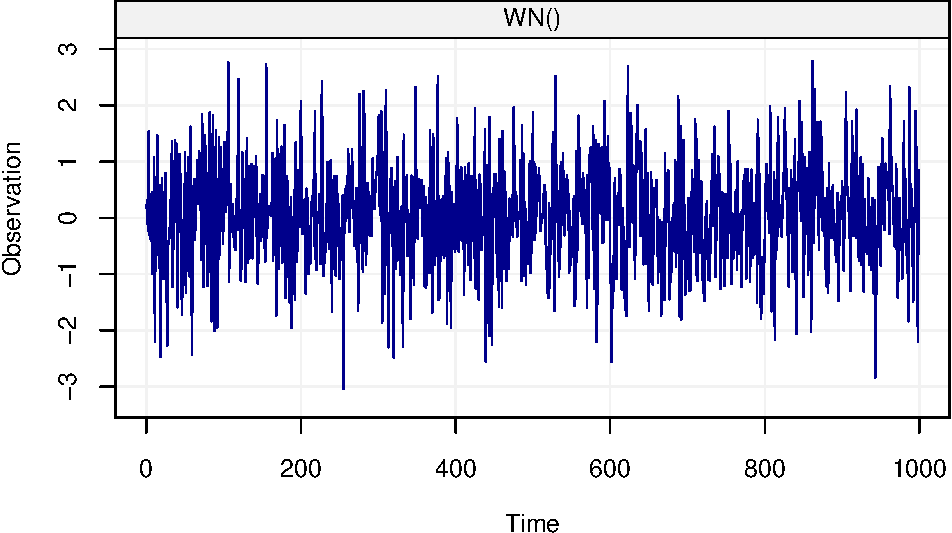
\includegraphics{ts_files/figure-latex/example_WN-1.pdf}

This model can be found in different applied settings and is often
accompanied by some of the models presented in the following paragraphs.

\subsection{Random Walk}\label{rw}

The term \emph{random walk} was first introduced by Karl Pearson in the
early nineteen-hundreds and a wide range of random walk models have been
defined over the years. For example, one of the simplest forms of a
random walk process can be explained as follows: suppose that you are
walking on campus and your next step can either be to your left, your
right, forward or backward (each with equal probability). Two
realizations of such processes are represented below:

\begin{Shaded}
\begin{Highlighting}[]
\KeywordTok{set.seed}\NormalTok{(}\DecValTok{5}\NormalTok{)}
\KeywordTok{RW2dimension}\NormalTok{(}\DataTypeTok{steps =} \DecValTok{10}\OperatorTok{^}\DecValTok{2}\NormalTok{)}
\end{Highlighting}
\end{Shaded}

\begin{center}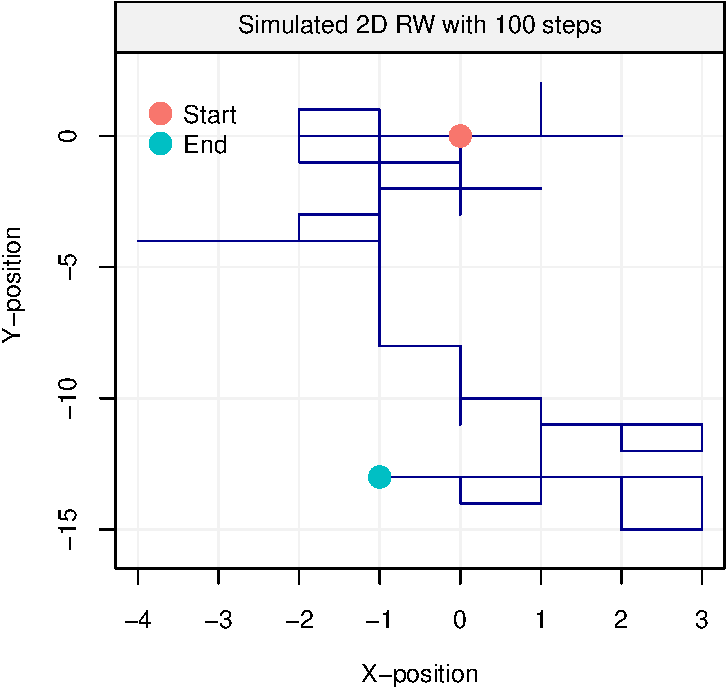
\includegraphics{ts_files/figure-latex/RW2d-1} \end{center}

\begin{Shaded}
\begin{Highlighting}[]
\KeywordTok{RW2dimension}\NormalTok{(}\DataTypeTok{steps =} \DecValTok{10}\OperatorTok{^}\DecValTok{4}\NormalTok{)}
\end{Highlighting}
\end{Shaded}

\begin{center}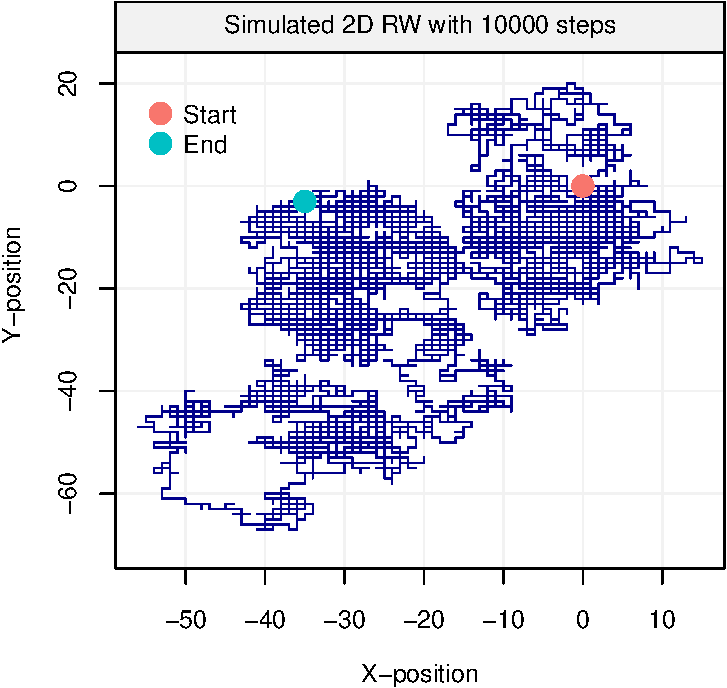
\includegraphics{ts_files/figure-latex/RW2d-2} \end{center}

Such processes inspired Karl Pearson's famous quote that

\begin{quote}
``\emph{the most likely place to find a drunken walker is somewhere near
his starting point.}''
\end{quote}

Empirical evidence of this phenomenon is not too hard to find on a
Friday or Saturday night. This two-dimensional process may easily be
extended to three dimensions and a simulated example of such a process
is presented in the animation below:

\includegraphics{asset/rw3.gif}

In this text, we only consider one very specific form of random walk,
namely the Gaussian random walk which can be defined as:

\[X_t = X_{t-1} + W_t,\]

where \(W_t\) is a Gaussian white noise process with initial condition
\(X_0 = c\) (typically \(c = 0\).) This process can be expressed
differently by \emph{backsubstitution} as follows:

\[\begin{aligned}
  {X_t} &= {X_{t - 1}} + {W_t} \\
   &= \left( {{X_{t - 2}} + {W_{t - 1}}} \right) + {W_t} \\
   &= \vdots \\
  {X_t} &= \sum\limits_{i = 1}^t {{W_i}} + X_0 =  \sum\limits_{i = 1}^t {{W_i}} + c \\ 
\end{aligned} \]

A random variable following a random walk can therefore be expressed as
the cumulated sum of all the random variables that precede it. The code
below presents an example of how to simulate a such process.

\begin{Shaded}
\begin{Highlighting}[]
\NormalTok{n =}\StringTok{ }\DecValTok{1000}                               \CommentTok{# process length}
\NormalTok{gamma2 =}\StringTok{ }\DecValTok{1}                             \CommentTok{# innovation variance}
\NormalTok{Xt =}\StringTok{ }\KeywordTok{gen_gts}\NormalTok{(n, }\KeywordTok{RW}\NormalTok{(}\DataTypeTok{gamma2 =}\NormalTok{ gamma2))}
\KeywordTok{plot}\NormalTok{(Xt)}
\end{Highlighting}
\end{Shaded}

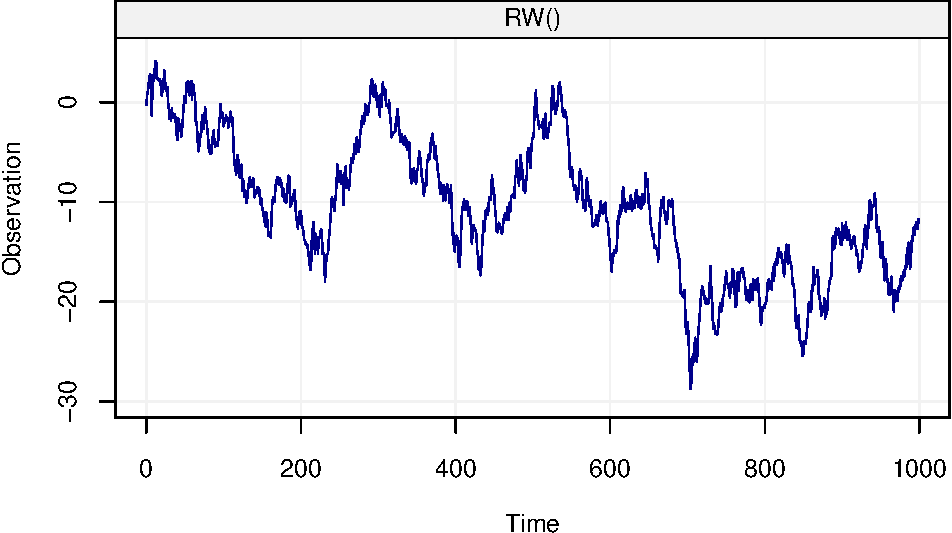
\includegraphics{ts_files/figure-latex/example_RW-1.pdf}

The random walk model is often used to explain phenomena in many
different areas one of which is finance where stock prices follow these
kind of processes.

\subsection{First-Order Autoregressive Model}\label{ar1}

A first-order autoregressive model or AR(1) is a generalization of both
the white noise and the random walk processes which are both special
cases of an AR(1). A (Gaussian) AR(1) process can be defined as

\[{X_t} = {\phi}{X_{t - 1}} + {W_t},\]

where \(W_t\) is a Gaussian white noise. Clearly, an AR(1) with
\(\phi = 0\) is a Gaussian white noise and when \(\phi = 1\) the process
becomes a random walk.

\BeginKnitrBlock{exercise}
\protect\hypertarget{exr:ar1realizations}{}{\label{exr:ar1realizations} }An
AR(1) is in fact a linear combination of past realisations of a white
noise \(W_t\) process. Indeed, we have

\[\begin{aligned}
 {X_t} &= {\phi_t}{X_{t - 1}} + {W_t} 
   = {\phi}\left( {{\phi}{X_{t - 2}} + {W_{t - 1}}} \right) + {W_t} \\
   &= \phi^2{X_{t - 2}} + {\phi}{W_{t - 1}} + {W_t} 
   = {\phi^t}{X_0} + \sum\limits_{i = 0}^{t - 1} {\phi^i{W_{t - i}}}.
\end{aligned}\]

Under the assumption of infinite past (i.e. \(t \in \mathbb{Z}\)) and
\(|\phi| < 1\), we obtain

\[X_t = \sum\limits_{i = 0}^{\infty} {\phi^i {W_{t - i}}},\]

since \(\operatorname{lim}_{i \to \infty} \; {\phi^i}{X_{t-i}} = 0\).
\EndKnitrBlock{exercise}

From the conclusion of the above the remark, you may have noticed how we
assume that the considered time series have zero expectation. The
following remark justifies this assumption.

\BeginKnitrBlock{exercise}
\protect\hypertarget{exr:ar1mean}{}{\label{exr:ar1mean} }We generally assume
that an AR(1), as well as other time series models, have zero mean. The
reason for this assumption is only to simplfy the notation but it is
easy to consider, for example, an AR(1) process around an arbitrary mean
\(\mu\), i.e.

\[\left(X_t - \mu\right) = \phi \left(X_{t-1} - \mu \right) + W_t,\]

which is of course equivalent to

\[X_t = \left(1 - \phi \right) \mu + \phi X_{t-1} + W_t.\]

Thus, we will generally only work with zero mean processes since adding
means is simple.
\EndKnitrBlock{exercise}

As for the previously presented models, we provide the code that gives
an example of how an AR(1) can be simulated.

\begin{Shaded}
\begin{Highlighting}[]
\NormalTok{n =}\StringTok{ }\DecValTok{1000}                              \CommentTok{# process length}
\NormalTok{phi =}\StringTok{ }\FloatTok{0.5}                             \CommentTok{# phi parameter}
\NormalTok{sigma2 =}\StringTok{ }\DecValTok{1}                            \CommentTok{# innovation variance}
\NormalTok{Xt =}\StringTok{ }\KeywordTok{gen_gts}\NormalTok{(n, }\KeywordTok{AR1}\NormalTok{(}\DataTypeTok{phi =}\NormalTok{ phi, }\DataTypeTok{sigma2 =}\NormalTok{ sigma2))}
\KeywordTok{plot}\NormalTok{(Xt)}
\end{Highlighting}
\end{Shaded}

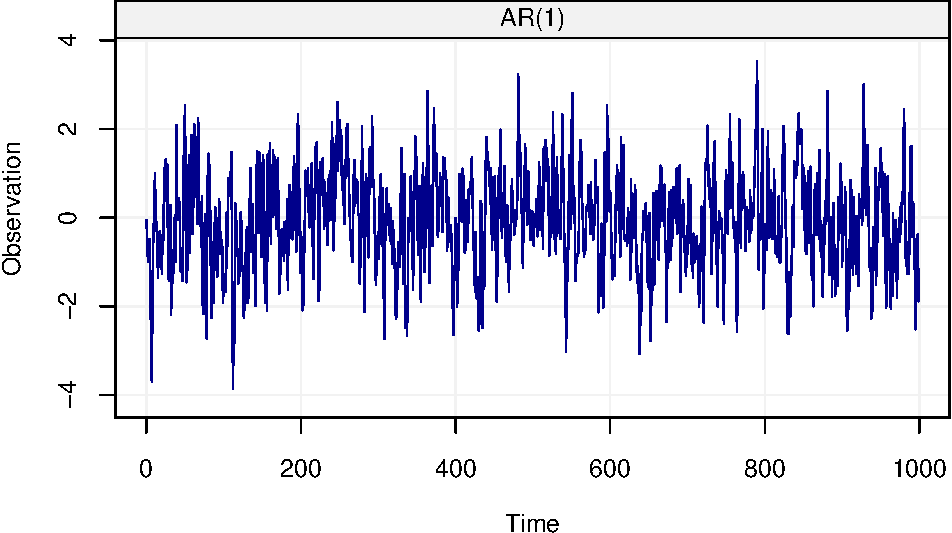
\includegraphics{ts_files/figure-latex/example_AR1-1.pdf}

The AR(1) model is one of the most popular and commonly used models in
many practical settings going from biology where it is used to explain
the evolution of gene expressions to economics where it is used to model
macroeconomic trends.

\subsection{Moving Average Process of Order 1}\label{ma1}

As seen in the previous example, an AR(1) can be expressed as a linear
combination of all past observations of the white noise process
\((W_t)\). In a similar manner we can (in some sense) describe the
moving average process of order 1 or MA(1) as a ``truncated'' version of
an AR(1). This model is defined as

\begin{equation} 
  X_t = \theta W_{t-1} + W_t,
\end{equation}

where (again) \(W_t\) denotes a Gaussian white noise process. As we will
see further on, as for the AR(1) model, this model can also be
represented as a linear combination of past observations but it has
different characteristics which can capture different types of dynamics
in various practical cases.

An example on how to generate an MA(1) is given below:

\begin{Shaded}
\begin{Highlighting}[]
\NormalTok{n =}\StringTok{ }\DecValTok{1000}                              \CommentTok{# process length}
\NormalTok{sigma2 =}\StringTok{ }\DecValTok{1}                            \CommentTok{# innovation variance}
\NormalTok{theta =}\StringTok{ }\FloatTok{0.5}                           \CommentTok{# theta parameter}
\NormalTok{Xt =}\StringTok{ }\KeywordTok{gen_gts}\NormalTok{(n, }\KeywordTok{MA1}\NormalTok{(}\DataTypeTok{theta =}\NormalTok{ theta, }\DataTypeTok{sigma2 =}\NormalTok{ sigma2))}
\KeywordTok{plot}\NormalTok{(Xt)}
\end{Highlighting}
\end{Shaded}

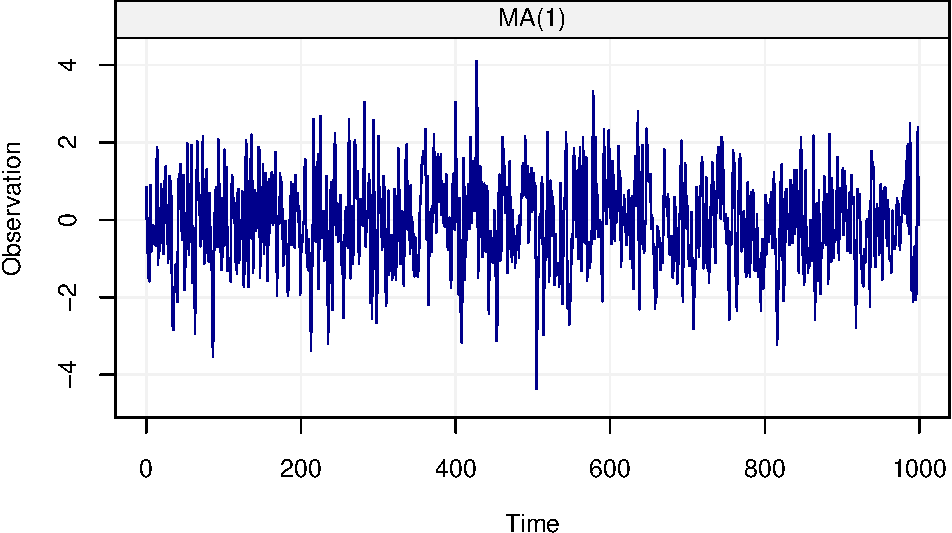
\includegraphics{ts_files/figure-latex/example_MA1-1.pdf}

The use of this model is widespread, especially combined with the AR(1)
model, and can be found in fields such as engineering where it is often
used for signal processing.

\subsection{Linear Drift}\label{drift}

A linear drift is a very simple deterministic time series model which
can be expressed as

\[X_t = X_{t-1} + \omega, \]

where \(\omega\) is a constant and with the initial condition
\(X_0 = c\), where \(c\) is an arbitrary constant (typically \(c = 0\)).
This process can be expressed in a more familiar form as follows:

\[
  {X_t} = {X_{t - 1}} + \omega 
   = \left( {{X_{t - 2}} + \omega} \right) + \omega 
   = t{\omega} + c . \]

Therefore, a (linear) drift corresponds to a simple linear model with
slope \(\omega\) and intercept \(c\).

\BeginKnitrBlock{exercise}
\protect\hypertarget{exr:remdrift}{}{\label{exr:remdrift} }You may argue
that the definition of this model is not useful since it constitutes a
simple linear model. However this model is often accompanied by other
time series models (such as the ones presented earlier) and its
estimation can be greatly improved when considered in conjunction with
the other models.
\EndKnitrBlock{exercise}

Given its simple form, a linear drift can simply be generated using the
code below:

\begin{Shaded}
\begin{Highlighting}[]
\NormalTok{n =}\StringTok{ }\DecValTok{100}                               \CommentTok{# process length}
\NormalTok{omega =}\StringTok{ }\FloatTok{0.5}                           \CommentTok{# slope parameter}
\NormalTok{Xt =}\StringTok{ }\KeywordTok{gen_gts}\NormalTok{(n, }\KeywordTok{DR}\NormalTok{(}\DataTypeTok{omega =}\NormalTok{ omega))}
\KeywordTok{plot}\NormalTok{(Xt)}
\end{Highlighting}
\end{Shaded}

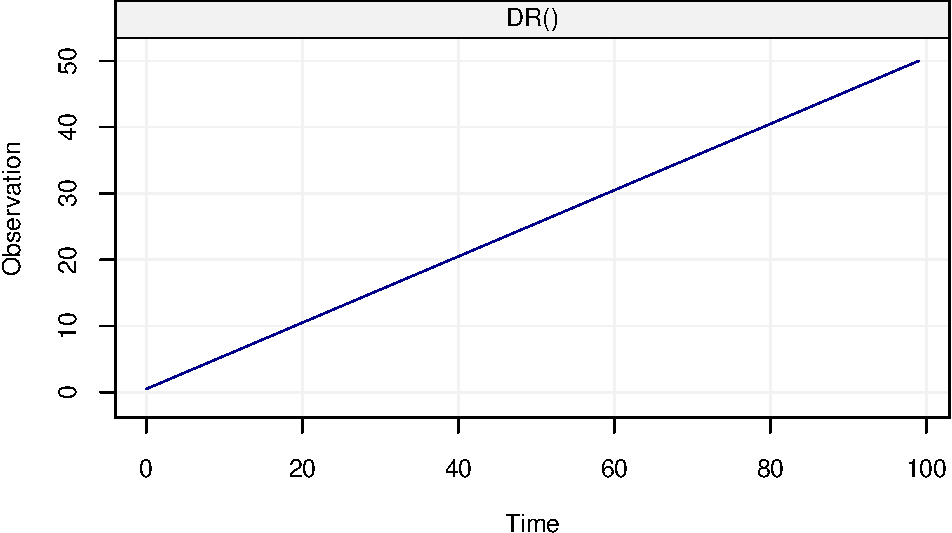
\includegraphics{ts_files/figure-latex/example_Drift-1.pdf}

This time series model is widely used in different areas of signal
analysis where mechanical systems and measuring devices can be
characterized by this type of behaviour.

\section{Composite Stochastic Processes}\label{lts}

In the previous paragraphs we defined and briefly discussed the basic
time series models that can individually be used to describe and predict
a wide range of phenomena in a variety of fields of application.
However, their capability of capturing and explaining the different
behaviours of phenomena through time increases considerably when they
are combined to form so-called \emph{composite models} (or composite
processes). A composite (stochastic) process can be defined as the sum
of underlying (or latent) time series models and in the rest of this
book we will use the term \emph{latent time series models} to refer to
these kinds of models. A simple example of such a model is given by

\[\begin{aligned}
Y_t &= Y_{t-1} + W_t + \delta\\
X_t &= Y_t + Z_t,
\end{aligned}\]

where \(W_t\) and \(Z_t\) are two independent Gaussian white noise
processes. This model is often used as a first basis to approximate the
number of individuals in the context ecological population dynamics. For
example, suppose we want to study the population of Chamois in the Swiss
Alps. Let \(Y_t\) denote the ``true'' number of individuals in this
population at time \(t\). It is reasonable to assume that the number of
individuals at time \(t\) (\(Y_t\)) is (approximately) the population at
the previous time \(t-1\) (e.g the previous year) plus a random
variation and a drift. This random variation is due to the natural
randomness in ecological population dynamics and reflects changes such
as the number of predators, the abundance of food, or weather
conditions. On the other hand, ecological \emph{drift} is often of
particular interest for ecologists as it can be used to determine the
``long'' term trends of the population (e.g.~if the population is
increasing, decreasing, or stable). Of course, \(Y_t\) (the number of
individauls) is typically unknown and we observe a noisy version of it,
denoted as \(X_t\). This process corresponds to the true population plus
a measurement error since some individuals may not be observed while
others may have been counted several times. Interestingly, this process
can clearly be expressed as a \emph{latent time series model} (or
composite stochastic process) as follows:

\[\begin{aligned}
R_t &= R_{t-1} + W_t \\
S_t &= \delta t \\
X_t &= R_t + S_t + Z_t,
\end{aligned}\]

where \(R_t\), \(S_t\) and \(Z_t\) denote, respectively, a random walk,
a drift, and a white noise. The code below can be used to simulate such
data:

\begin{Shaded}
\begin{Highlighting}[]
\NormalTok{n =}\StringTok{ }\DecValTok{1000}                                \CommentTok{# process length}
\NormalTok{delta =}\StringTok{ }\FloatTok{0.005}                           \CommentTok{# delta parameter (drift)}
\NormalTok{sigma2 =}\StringTok{ }\DecValTok{10}                             \CommentTok{# variance parameter (white noise)}
\NormalTok{gamma2 =}\StringTok{ }\FloatTok{0.1}                            \CommentTok{# innovation variance (random walk)}
\NormalTok{model =}\StringTok{ }\KeywordTok{WN}\NormalTok{(}\DataTypeTok{sigma2 =}\NormalTok{ sigma2) }\OperatorTok{+}\StringTok{ }\KeywordTok{RW}\NormalTok{(}\DataTypeTok{gamma2 =}\NormalTok{ gamma2) }\OperatorTok{+}\StringTok{ }\KeywordTok{DR}\NormalTok{(}\DataTypeTok{omega =}\NormalTok{ delta)}
\NormalTok{Xt =}\StringTok{ }\KeywordTok{gen_lts}\NormalTok{(}\DataTypeTok{n =}\NormalTok{ n, }\DataTypeTok{model =}\NormalTok{ model)}
\KeywordTok{plot}\NormalTok{(Xt)}
\end{Highlighting}
\end{Shaded}

\begin{center}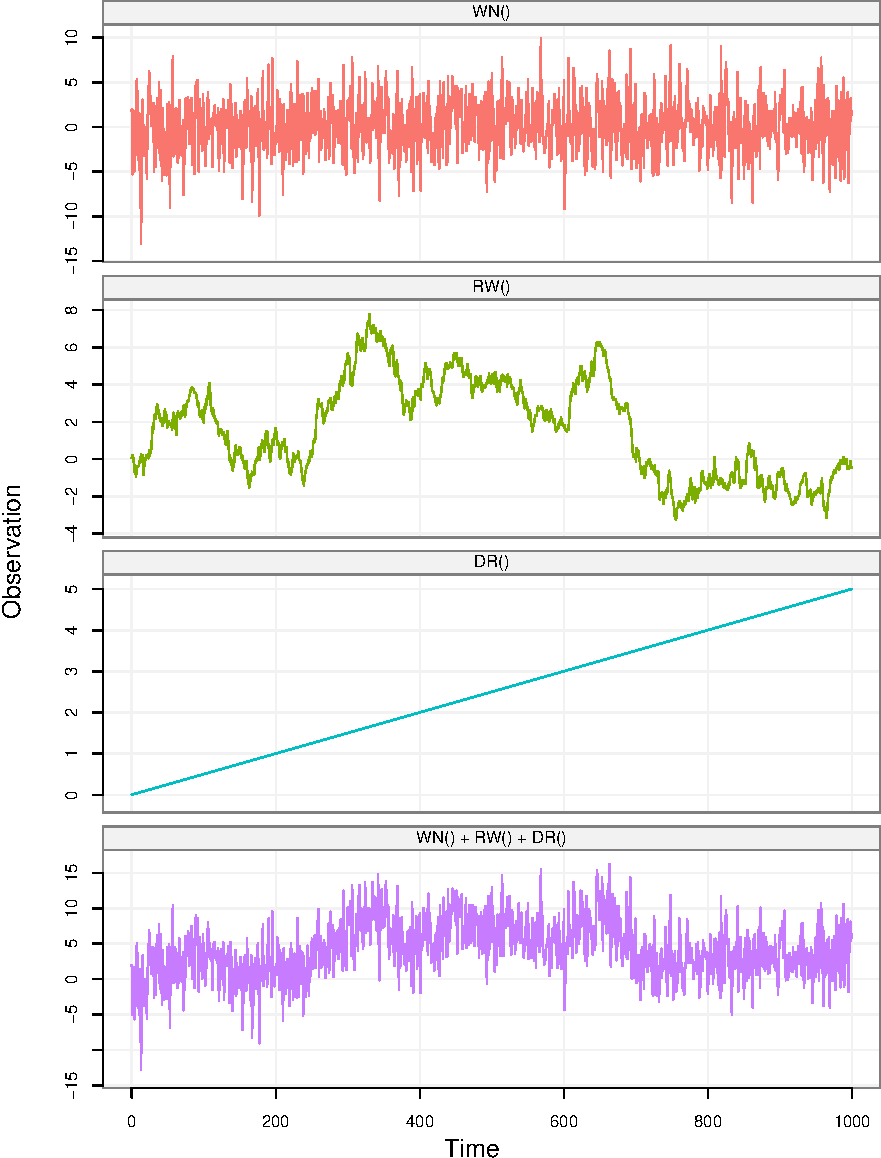
\includegraphics{ts_files/figure-latex/examplecomposite-1} \end{center}

In the above graph, the first three plots represent the latent
(unobserved) processes (i.e.~white noise, random walk, and drift) and
the last one represents the sum of the three (i.e. \((X_t)\)).

Let us consider a real example where these latent processes are useful
to describe (and predict) the behavior of economic variables such as
Personal Saving Rates (PSR). A process that is used for these settings
is the ``random-walk-plus-noise'' model, meaning that the data can be
explained by a random walk process in addition to which we observe some
other process (e.g. a white noise model, an autoregressive model such as
an AR(1), etc.). The PSR taken from the Federal Reserve of St.~Louis
from January 1, 1959, to May 1, 2015, is presented in the following
plot:

\begin{Shaded}
\begin{Highlighting}[]
\CommentTok{# Load savingrt dataset}
\KeywordTok{data}\NormalTok{(}\StringTok{"savingrt"}\NormalTok{)}
\CommentTok{# Simulate based on data}
\NormalTok{savingrt =}\StringTok{ }\KeywordTok{gts}\NormalTok{(}\KeywordTok{as.vector}\NormalTok{(savingrt), }\DataTypeTok{start =} \DecValTok{1959}\NormalTok{, }\DataTypeTok{freq =} \DecValTok{12}\NormalTok{, }\DataTypeTok{unit_ts =} \StringTok{"%"}\NormalTok{, }
            \DataTypeTok{name_ts =} \StringTok{"Saving Rates"}\NormalTok{, }\DataTypeTok{data_name =} \StringTok{"US Personal Saving Rates"}\NormalTok{)}
\CommentTok{# Plot savingrt simulation}
\KeywordTok{plot}\NormalTok{(savingrt)}
\end{Highlighting}
\end{Shaded}

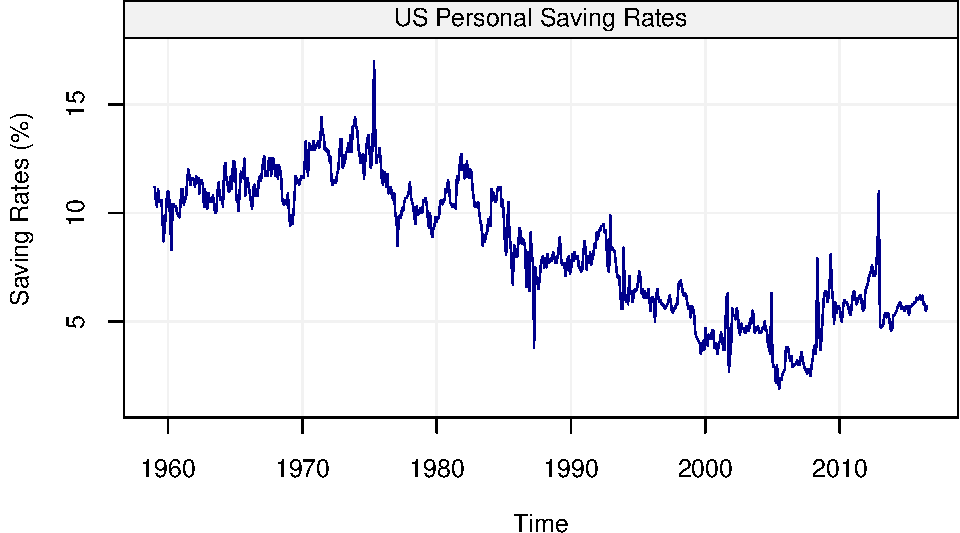
\includegraphics{ts_files/figure-latex/example_PSR-1.pdf}

It can be observed that the mean of this process seems to vary over
time, suggesting that a random walk can indeed be considered as a
possible model to explain this data. In addition, aside from some
``spikes'' and occasional sudden changes, the observations appear to
gradually change from one time point to the other, suggesting that some
other form of dependence between them could exist.

\chapter{Fundamental Properties of Time Series}\label{fundtimeseries}

\begin{quote}
``\emph{One of the first things taught in introductory statistics
textbooks is that correlation is not causation. It is also one of the
first things forgotten.}'' -- Thomas Sowell
\end{quote}

\BeginKnitrBlock{rmdimportant}
To make use of the R code within this chapter you will need to install
(if not already done) and load the following libraries:

\begin{itemize}
\tightlist
\item
  \href{https://cran.r-project.org/web/packages/quantmod/index.html}{quantmod};
\item
  \href{http://simts.smac-group.com/}{simts};
\item
  \href{https://cran.r-project.org/web/packages/astsa/index.html}{astsa};
\item
  \href{https://cran.r-project.org/web/packages/robcor/index.html}{robcor}.

  \EndKnitrBlock{rmdimportant}
\end{itemize}

In this chapter we will discuss and formalize how knowledge about
\(X_{t-1}\) (or more generally about all the information from the past,
\(\Omega_t\)) can provide us with some information about the properties
of \(X_t\). In particular, we will consider the correlation (or
covariance) of \(X_t\) at different times such as
\(\text{corr} \left(X_t, X_{t+h}\right)\). This ``form'' of correlation
(covariance) is called the \emph{autocorrelation}
(\emph{autocovariance}) and is a very useful tool in time series
analysis. However, if we do not assume that a time series is
characterized by a certain form of ``stability'', it would be rather
difficult to estimate \(\text{corr} \left(X_t, X_{t+h}\right)\) as this
quantity would depend on both \(t\) and \(h\) leading to more parameters
to estimate than observations available. Therefore, the concept of
\emph{stationarity} (which we will describe further on) is convenient in
this context as it allows (among other things) to assume that

\[\text{corr} \left(X_t, X_{t+h}\right) = \text{corr} \left(X_{t+j}, X_{t+h+j}\right), \;\;\; \text{for all $j$},\]

implying that the autocorrelation (or autocovariance) is only a function
of the lag between observations, rather than time itself. We will first
discuss the concept of autocorrelation in time series, then we will
discuss stationarity which will then allow us to adequately define and
study estimators of the autocorrelation functions. Before moving on, it
is helpful to remember that correlation (or autocorrelation) is only
appropriate to measure a very specific kind of dependence, i.e.~linear
dependence. There are many other forms of dependence as illustrated in
the bottom panels of the graph below, which all have a (true) zero
correlation:

\begin{figure}

{\centering 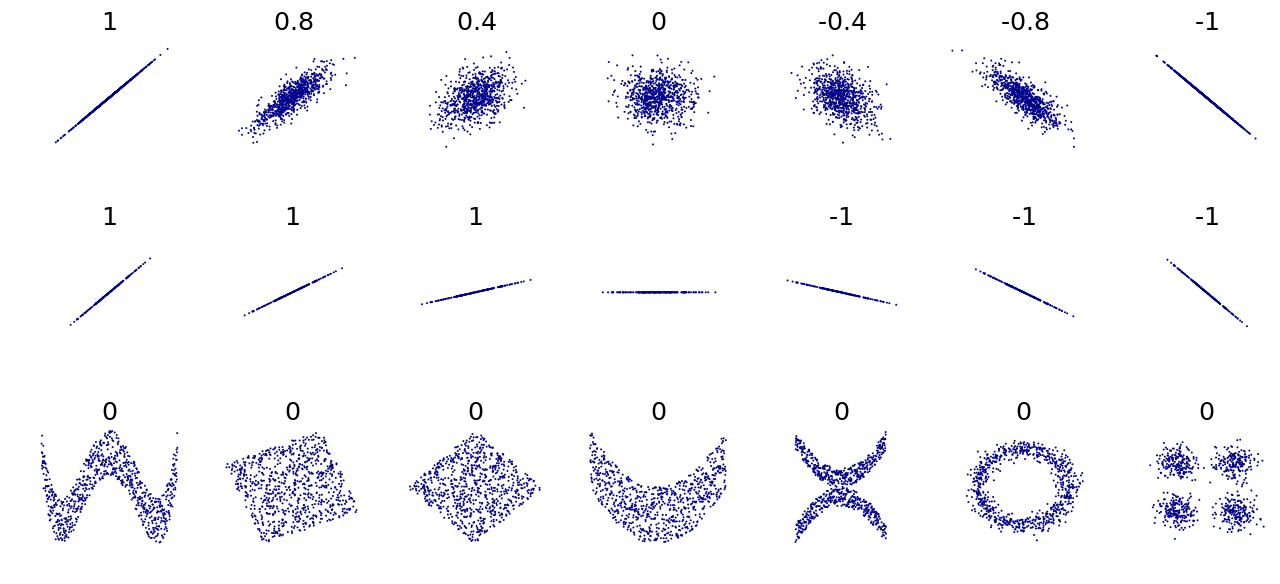
\includegraphics{images/corr_example} 

}

\caption{Different forms of dependence and their Pearson's r values}\label{fig:correxample}
\end{figure}

Several other metrics have been introduced in the literature to assess
the degree of ``dependence'' of two random variables, however this goes
beyond the material discussed in this chapter.

\section{The Autocorrelation and Autocovariance
Functions}\label{the-autocorrelation-and-autocovariance-functions}

We will introduce the autocorrelation function by first defining the
\textbf{autocovariance function}.

\BeginKnitrBlock{definition}
\protect\hypertarget{def:acvf}{}{\label{def:acvf} }The \emph{autocovariance
function} of a series \((X_t)\) is defined as

\[{\gamma_x}\left( {t,t+h} \right) \equiv \text{cov} \left( {{X_t},{X_{t+h}}} \right),\]
\EndKnitrBlock{definition}

where the definition of covariance is given by:

\[
    \text{cov} \left( {{X_t},{X_{t+h}}} \right) \equiv \mathbb{E}\left[ {{X_t}{X_{t+h}}} \right] - \mathbb{E}\left[ {{X_t}} \right]\mathbb{E}\left[ {{X_{t+h}}} \right].
    \]

Similarly, the above expectations are defined as:

\[\begin{aligned}
     \mathbb{E}\left[ {{X_t}} \right] &\equiv \int\limits_{ - \infty }^\infty  {x \cdot {f_t}\left( x \right)dx},  \\
     \mathbb{E}\left[ {{X_t}{X_{t+h}}} \right] &\equiv \int\limits_{ - \infty }^\infty  {\int\limits_{ - \infty }^\infty  {{x_1}{x_2} \cdot f_{t,t+h}\left( {{x_1},{x_2}} \right)d{x_1}d{x_2}} } ,
     \end{aligned} \]

where \({f_t}\left( x \right)\) and
\(f_{t,t+h}\left( {{x_1},{x_2}} \right)\) denote, respectively, the
density of \(X_t\) and the joint density of the pair \((X_t, X_{t+h})\).
Considering the notation used above, it should be clear that \(X_t\) is
assumed to be a continous random variable. Since we generally consider
stochastic processes with constant zero mean, we often have

\[{\gamma_x}\left( {t,t+h} \right) = \mathbb{E}\left[X_t X_{t+h} \right]. \]

In addition, in the context of this book we will normally drop the
subscript referring to the time series (i.e. \(x\) in this case) if it
is clear from the context which time series the autocovariance refers
to. For example, we generally use \({\gamma}\left( {t,t+h} \right)\)
instead of \({\gamma_x}\left( {t,t+h} \right)\). Moreover, the notation
is even further simplified when the covariance of \(X_t\) and
\(X_{t+h}\) is the same as that of \(X_{t+j}\) and \(X_{t+h+j}\) (for
all \(j\)), i.e.~the covariance depends only on the time between
observations and not on the specific time \(t\). This is consequence of
an important property called \emph{stationarity} that was mentioned
earlier and will be discussed in the next section. In this case, we
simply use to following notation:

\[\gamma \left( {h} \right) = \text{cov} \left( X_t , X_{t+h} \right). \]

This is the definition of autocovariance that will be used from this
point onwards and therefore this notation will generally be used
throughout the text thereby implying certain properties for the process
\((X_t)\) (i.e.~stationarity) . With this in mind, several remarks can
be made on the autocovariance function:

\begin{enumerate}
\def\labelenumi{\arabic{enumi}.}
\tightlist
\item
  The autocovariance function is \emph{symmetric}. That is,
  \({\gamma}\left( {h} \right) = {\gamma}\left( -h \right)\) since
  \(\text{cov} \left( {{X_t},{X_{t+h}}} \right) = \text{cov} \left( X_{t+h},X_{t} \right)\).
\item
  The autocovariance function ``contains'' the variance of the process
  as \(\text{var} \left( X_{t} \right) = {\gamma}\left( 0 \right)\).
\item
  We have that \(|\gamma(h)| \leq \gamma(0)\) for all \(h\). The proof
  of this inequality is direct and follows from the Cauchy-Schwarz
  inequality, i.e. \[ \begin{aligned}
    \left(|\gamma(h)| \right)^2 &= \gamma(h)^2 = \left(\mathbb{E}\left[\left(X_t - \mathbb{E}[X_t] \right)\left(X_{t+h} - \mathbb{E}[X_{t+h}] \right)\right]\right)^2\\
    &\leq \mathbb{E}\left[\left(X_t - \mathbb{E}[X_t] \right)^2 \right] \mathbb{E}\left[\left(X_{t+h} - \mathbb{E}[X_{t+h}] \right)^2 \right] =  \gamma(0)^2. 
    \end{aligned}
    \]
\item
  Just as any covariance, \({\gamma}\left( {h} \right)\) is ``scale
  dependent'' since \({\gamma}\left( {h} \right) \in \mathbb{R}\), or
  \(-\infty \le {\gamma}\left( {h} \right) \le +\infty\). We therefore
  have:
\end{enumerate}

\begin{itemize}
\tightlist
\item
  if \(\left| {\gamma}\left( {h} \right) \right|\) is ``close'' to zero,
  then \(X_t\) and \(X_{t+h}\) are ``weakly'' (linearly) dependent;
\item
  if \(\left| {\gamma}\left( {h} \right) \right|\) is ``far'' from zero,
  then the two random variables present a ``strong'' (linear)
  dependence. However it is generally difficult to asses what ``close''
  and ``far'' from zero means in this case.
\end{itemize}

\begin{enumerate}
\def\labelenumi{\arabic{enumi}.}
\setcounter{enumi}{4}
\tightlist
\item
  \({\gamma}\left( {h} \right)=0\) does not imply that \(X_t\) and
  \(X_{t+h}\) are independent but simply that they are uncorrelated. The
  independence is only implied by \({\gamma}\left( {h} \right)=0\) in
  the jointly Gaussian case.
\end{enumerate}

As hinted in the introduction, an important related statistic is the
correlation of \(X_t\) with \(X_{t+h}\) or \emph{autocorrelation}, which
is defined as

\[\rho \left(  h \right) = \text{corr}\left( {{X_t},{X_{t + h}}} \right) = \frac{{\text{cov}\left( {{X_t},{X_{t + h}}} \right)}}{{{\sigma _{{X_t}}}{\sigma _{{X_{t + h}}}}}} = \frac{\gamma(h) }{\gamma(0)}.\]

Similarly to \(\gamma(h)\), it is important to note that the above
notation implies that the autocorrelation function is only a function of
the lag \(h\) between observations. Thus, autocovariances and
autocorrelations are one possible way to describe the joint distribution
of a time series. Indeed, the correlation of \(X_t\) with \(X_{t+h}\) is
an obvious measure of how \emph{persistent} a time series is.

Remember that just as with any correlation:

\begin{enumerate}
\def\labelenumi{\arabic{enumi}.}
\tightlist
\item
  \(\rho \left( h \right)\) is ``scale free'' so it is much easier to
  interpret than \(\gamma(h)\).
\item
  \(|\rho \left( h \right)| \leq 1\) since
  \(|\gamma(h)| \leq \gamma(0)\).
\item
  \textbf{Causation and correlation are two very different things!}
\end{enumerate}

\subsection{A Fundamental
Representation}\label{a-fundamental-representation}

Autocovariances and autocorrelations also turn out to be very useful
tools as they are one of the \emph{fundamental representations} of time
series. Indeed, if we consider a zero mean normally distributed process,
it is clear that its joint distribution is fully characterized by the
autocovariances \(\mathbb{E}[X_t X_{t+h}]\) (since the joint probability
density only depends of these covariances). Once we know the
autocovariances we know \emph{everything} there is to know about the
process and therefore:

\begin{quote}
if two (Gaussian) processes have the same autocovariance function, then
they are the same process.
\end{quote}

\subsection{Admissible Autocorrelation Functions
😱}\label{admissible-autocorrelation-functions}

Since the autocorrelation function is one of the fundamental
representations of time series, it implies that one might be able to
define a stochastic process by picking a set of autocorrelation values
(assuming for example that \(\text{var}(X_t) = 1\)). However, it turns
out that not every collection of numbers, say
\(\{\rho_1, \rho_2, ...\},\) can represent the autocorrelation of a
process. Indeed, two conditions are required to ensure the validity of
an autocorrelation sequence:

\begin{enumerate}
\def\labelenumi{\arabic{enumi}.}
\tightlist
\item
  \(\operatorname{max}_j \; \left| \rho_j \right| \leq 1\).
\item
  \(\text{var} \left[\sum_{j = 0}^\infty \alpha_j X_{t-j} \right] \geq 0 \;\)
  for all \(\{\alpha_0, \alpha_1, ...\}\).
\end{enumerate}

The first condition is obvious and simply reflects the fact that
\(|\rho \left( h \right)| \leq 1\) but the second is far more difficult
to verify. To further our understanding of the latter we let
\(\alpha_j = 0\) for \(j > 1\) and see that in this case the second
condition implies that

\[\text{var} \left[ \alpha_0 X_{t} + \alpha_1 X_{t-1}  \right] = \gamma_0 \begin{bmatrix}
   \alpha_0 & \alpha_1
   \end{bmatrix}   \begin{bmatrix}
   1 & \rho_1\\
   \rho_1 & 1
   \end{bmatrix} \begin{bmatrix}
   \alpha_0 \\
   \alpha_1
   \end{bmatrix} \geq 0, \]

where \(\gamma_0\) is a more compact notation for \(\gamma(0)\). Thus,
the matrix

\[ \boldsymbol{A}_1 = \begin{bmatrix}
  1 & \rho_1\\
  \rho_1 & 1
  \end{bmatrix}, \]

must be positive semi-definite. Taking the determinant we have

\[\operatorname{det} \left(\boldsymbol{A}_1\right) = 1 - \rho_1^2, \]

implying that the condition \(|\rho_1| \leq 1\) must be respected. Now,
let \(\alpha_j = 0\) for \(j > 2\), then we must verify that:

\[\text{var} \left[ \alpha_0 X_{t} + \alpha_1 X_{t-1}  + \alpha_2 X_{t-2} \right] = \gamma_0 \begin{bmatrix}
     \alpha_0 & \alpha_1 &\alpha_2
     \end{bmatrix}   \begin{bmatrix}
     1 & \rho_1 & \rho_2\\
     \rho_1 & 1 & \rho_1 \\
     \rho_2 & \rho_1 & 1
     \end{bmatrix} \begin{bmatrix}
     \alpha_0 \\
     \alpha_1 \\
     \alpha_2
     \end{bmatrix} \geq 0. \]

Again, this implies that the matrix

\[ \boldsymbol{A}_2 = \begin{bmatrix}
  1 & \rho_1 & \rho_2\\
  \rho_1 & 1 & \rho_1 \\
  \rho_2 & \rho_1 & 1
  \end{bmatrix}, \]

must be positive semi-definite and it is easy to verify that

\[\operatorname{det} \left(\boldsymbol{A}_2\right) = \left(1 - \rho_2 \right)\left(- 2 \rho_1^2 + \rho_2 + 1\right). \]

Thus, this implies that

\[\begin{aligned} &- 2 \rho_1^2 + \rho_2 + 1 \geq 0 \Rightarrow 1 \geq \rho_2 \geq 2 \rho_1^2 - 1 \\
   &\Rightarrow 1 - \rho_1^2 \geq \rho_2 - \rho_1^2 \geq -(1 - \rho_1^2)\\
   &\Rightarrow 1 \geq \frac{\rho_2 - \rho_1^2 }{1 - \rho_1^2} \geq -1.
   \end{aligned}\]

Therefore, \(\rho_1\) and \(\rho_2\) must lie in a parabolic shaped
region defined by the above inequalities as illustrated in Figure
\ref{fig:admissibility}.

\begin{figure}

{\centering 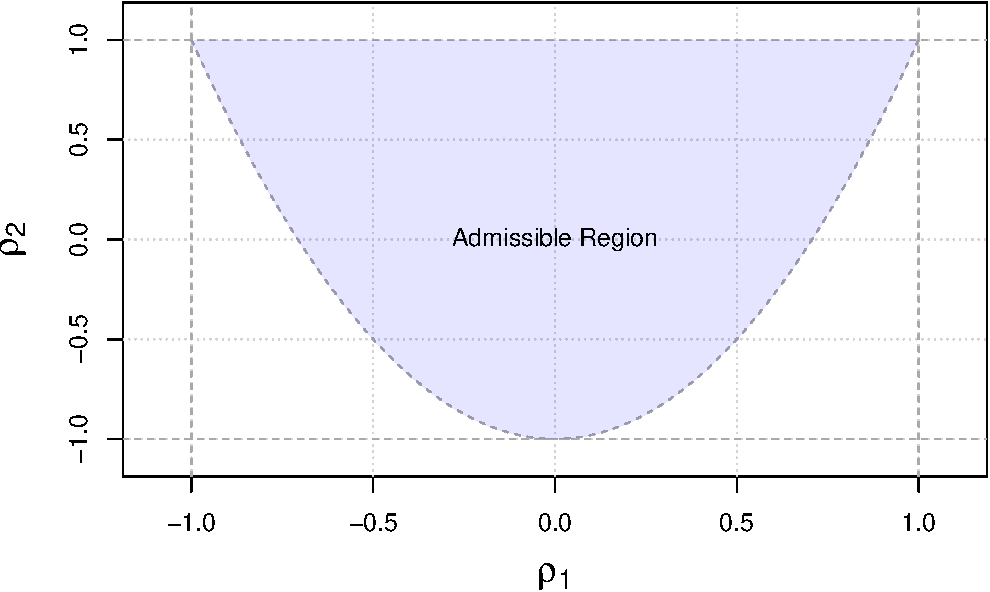
\includegraphics{ts_files/figure-latex/admissibility-1} 

}

\caption{Admissible autocorrelation functions}\label{fig:admissibility}
\end{figure}

From our derivation, it is clear that the restrictions on the
autocorrelation are very complicated, thereby justifying the need for
other forms of fundamental representation which we will explore later in
this text. Before moving on to the estimation of the autocorrelation and
autocovariance functions, we must first discuss the stationarity of
\((X_t)\), which will provide a convenient framework in which
\(\gamma(h)\) and \(\rho(h)\) can be used (rather that \(\gamma(t,t+h)\)
for example) and (easily) estimated.

\section{Stationarity}\label{stationary}

There are two kinds of stationarity that are commonly used. They are
defined as follows:

\BeginKnitrBlock{definition}
\protect\hypertarget{def:strongstationarity}{}{\label{def:strongstationarity}
}A process \((X_t)\) is \emph{strongly stationary} or \emph{strictly
stationary} if the joint probability distribution of
\((X_{t-h}, ..., X_t, ..., X_{t+h})\) is independent of \(t\) for all
\(t,h \in \mathbb{Z}\).
\EndKnitrBlock{definition}

\BeginKnitrBlock{definition}
\protect\hypertarget{def:weakstationarity}{}{\label{def:weakstationarity} }A
process \((X_t)\) is \emph{weakly stationary}, \emph{covariance
stationary} or \emph{second order stationary} if \(\mathbb{E}[X_t]\) and
\(\mathbb{E}[X_t^2]\) are finite and \(\mathbb{E}[X_t X_{t-h}]\) depends
only on \(h\) and not on \(t\) for all \(t,h \in \mathbb{Z}\).
\EndKnitrBlock{definition}

These types of stationarity are \emph{not equivalent} and the presence
of one kind of stationarity does not imply the other. That is, a time
series can be strongly stationary but not weakly stationary and vice
versa. In some cases, a time series can be both strongly and weakly
stationary and this occurs, for example, in the (jointly) Gaussian case.
Stationarity of \((X_t)\) matters because \emph{it provides the
framework in which averaging dependent data makes sense}, thereby
allowing us to easily obtain estimates for certain quantities such as
autocorrelation.

Several remarks and comments can be made on these definitions:

\begin{itemize}
\item
  As mentioned earlier, strong stationarity \emph{does not imply} weak
  stationarity. For example, an \(iid\) Cauchy process is strongly but
  not weakly stationary (why? 🤔).
\item
  Weak stationarity \emph{does not imply} strong stationarity. For
  example, consider the following weak white noise process:

  \begin{equation*}
  X_t = \begin{cases}
  U_{t}      & \quad \text{if } t \in \{2k:\, k\in \mathbb{Z} \}, \\
  V_{t}      & \quad \text{if } t \in \{2k+1:\, k\in \mathbb{Z} \},\\
  \end{cases}
  \end{equation*}

  where \({U_t} \mathop \sim \limits^{iid} N\left( {1,1} \right)\) and
  \({V_t}\mathop \sim \limits^{iid} \mathcal{E}\left( 1 \right)\) is a
  weakly stationary process that is \emph{not} strongly stationary.
\item
  Strong stationarity combined with bounded values of
  \(\mathbb{E}[X_t^2]\) \emph{implies} weak stationarity.
\item
  Weak stationarity combined with normally distributed processes
  \emph{implies} strong stationarity.
\end{itemize}

\BeginKnitrBlock{exercise}[Existence of moments]
\protect\hypertarget{exr:moment}{}{\label{exr:moment} \iffalse (Existence of
moments) \fi{} }It is important to note that, for a given value of \(r\)
and a random variable \(X\), the expected value \(\mathbb{E}[X^r]\) may
be infinite, or may not exist. If there exists an \(r \in \mathbb{N}^+\)
such that \(\mathbb{E}[|X|^r]\) exists and is bounded, then we have that
\(\mathbb{E}[X^j] < \infty\) for all \(j = 1,...,r\). This result is
implied by Jensen's inequality. Indeed, the function \(f(x) = x^k\) is
convex for \(x > 0\) and \(k > 1\), so we have
\[\mathbb{E}\left[|X |^j\right]^{\frac{r}{j}} \leq \mathbb{E}\left[(|X |^j)^{\frac{r}{j}}\right] = \mathbb{E}\left[|X|^r\right] < \infty.\]
Therefore, we obtain
\(\mathbb{E}[X^j] \leq \mathbb{E}[|X|^j] < \infty\).
\EndKnitrBlock{exercise}

\subsection{Assessing Weak Stationarity of Time Series
Models}\label{assessing-weak-stationarity-of-time-series-models}

It is important to understand how to verify if a postulated model is
(weakly) stationary. In order to do so, we must ensure that our model
satisfies the following three properties:

\begin{enumerate}
\def\labelenumi{\arabic{enumi}.}
\tightlist
\item
  \(\mathbb{E}\left[X_t \right] = \mu_t = \mu < \infty\),
\item
  \(\text{var}\left[X_t \right] = \sigma^2_t = \sigma^2 < \infty\),
\item
  \(\text{cov}\left(X_t, X_{t+h} \right) = \gamma \left(h\right)\)
  (i.e.~the autocovariance only depends on \(h\) and not on \(t\)).
\end{enumerate}

In the following examples, we evaluate the stationarity of the processes
introduced in Section \ref{basicmodels}.

\BeginKnitrBlock{example}[Gaussian White Noise]
\protect\hypertarget{exm:gwn}{}{\label{exm:gwn} \iffalse (Gaussian White
Noise) \fi{} }It is easy to verify that this process is stationary.
Indeed, we have:

\begin{enumerate}
\def\labelenumi{\arabic{enumi}.}
\tightlist
\item
  \(\mathbb{E}\left[ {{X_t}} \right] = 0\),
\item
  \(\gamma(0) = \sigma^2 < \infty\),\\
\item
  \(\gamma(h) = 0\) for \(|h| > 0\).

  \EndKnitrBlock{example}
\end{enumerate}

\BeginKnitrBlock{example}[Random Walk]
\protect\hypertarget{exm:srw}{}{\label{exm:srw} \iffalse (Random Walk) \fi{}
}To evaluate the stationarity of this process, we first derive its
properties:

\begin{enumerate}
\def\labelenumi{\arabic{enumi}.}
\tightlist
\item
  We begin by calculating the expectation of the process: \[
    \mathbb{E}\left[ {{X_t}} \right] = \mathbb{E}\left[ {{X_{t - 1}} + {W_t}} \right]
    = \mathbb{E}\left[ {\sum\limits_{i = 1}^t {{W_i}}  + {X_0}} \right] 
    = \mathbb{E}\left[ {\sum\limits_{i = 1}^t {{W_i}} } \right] + {c} 
    = c.  \]
\end{enumerate}

Observe that the mean obtained is constant since it depends only on the
value of the first term in the sequence.

\begin{enumerate}
\def\labelenumi{\arabic{enumi}.}
\setcounter{enumi}{1}
\item
  Next, after finding the mean to be constant, we calculate the variance
  to check stationarity: \[\begin{aligned}
   \text{var}\left( {{X_t}} \right) &= \text{var}\left( {\sum\limits_{i = 1}^t {{W_t}}  + {X_0}} \right) 
   = \text{var}\left( {\sum\limits_{i = 1}^t {{W_i}} } \right) + \underbrace {\text{var}\left( {{X_0}} \right)}_{= 0} \\
   &= \sum\limits_{i = 1}^t {\text{var}\left( {{W_i}} \right)} 
   = t \sigma_w^2,
   \end{aligned}\] where \(\sigma_w^2 = \text{var}(W_t)\). Therefore,
  the variance depends on time \(t\), contradicting our second property.
  Moreover, we have:
  \[\mathop {\lim }\limits_{t \to \infty } \; \text{var}\left(X_t\right) = \infty.\]
  This process is therefore not weakly stationary.
\item
  Regarding the autocovariance of a random walk, we have:
  \[\begin{aligned}
   \gamma \left( h \right) &= \text{cov}\left( {{X_t},{X_{t + h}}} \right) 
   = \text{cov}\left( {\sum\limits_{i = 1}^t {{W_i}} ,\sum\limits_{j = 1}^{t + h} {{W_j}} } \right) \\ 
   &= \min \left( {t,t + h} \right)\sigma _w^2
   = \left( {t + \min \left( {0,h} \right)} \right)\sigma _w^2,
   \end{aligned} \] which further illustrates the non-stationarity of
  this process.
\end{enumerate}

Moreover, the autocorrelation of this process is given by

\[\rho (h) = \frac{t + \min \left( {0,h} \right)}{\sqrt{t}\sqrt{t+h}},\]

implying (for a fixed \(h\)) that

\[\mathop {\lim }\limits_{t \to \infty } \; \rho(h) = 1.\]

Note that using \(\gamma (h)\) and \(\rho (h)\) in this context is
actually an abuse of notation since both of these quantites are a
function of \(h\) and \(t\) for a random walk process.
\EndKnitrBlock{example}

In the following simulated example, we illustrate the non-stationary
feature of such a process:

\begin{Shaded}
\begin{Highlighting}[]
\CommentTok{# Number of simulated processes}
\NormalTok{B =}\StringTok{ }\DecValTok{200}

\CommentTok{# Length of random walks}
\NormalTok{n =}\StringTok{ }\DecValTok{1000}

\CommentTok{# Output matrix}
\NormalTok{out =}\StringTok{ }\KeywordTok{matrix}\NormalTok{(}\OtherTok{NA}\NormalTok{,B,n)}

\CommentTok{# Set seed for reproducibility}
\KeywordTok{set.seed}\NormalTok{(}\DecValTok{6182}\NormalTok{)}

\CommentTok{# Simulate Data}
\ControlFlowTok{for}\NormalTok{ (i }\ControlFlowTok{in} \KeywordTok{seq_len}\NormalTok{(B))\{}
  \CommentTok{# Simulate random walk}
\NormalTok{  Xt =}\StringTok{ }\KeywordTok{gen_gts}\NormalTok{(n, }\KeywordTok{RW}\NormalTok{(}\DataTypeTok{gamma =} \DecValTok{1}\NormalTok{))}
  
  \CommentTok{# Store process}
\NormalTok{  out[i,] =}\StringTok{ }\NormalTok{Xt}
\NormalTok{\}}

\CommentTok{# Plot random walks}
\KeywordTok{plot}\NormalTok{(}\OtherTok{NA}\NormalTok{, }\DataTypeTok{xlim =} \KeywordTok{c}\NormalTok{(}\DecValTok{1}\NormalTok{,n), }\DataTypeTok{ylim =} \KeywordTok{range}\NormalTok{(out), }\DataTypeTok{xlab =} \StringTok{"Time"}\NormalTok{, }\DataTypeTok{ylab =} \StringTok{" "}\NormalTok{)}
\KeywordTok{grid}\NormalTok{()}
\NormalTok{color =}\StringTok{ }\KeywordTok{sample}\NormalTok{(}\KeywordTok{topo.colors}\NormalTok{(B, }\DataTypeTok{alpha =} \FloatTok{0.5}\NormalTok{))}
\KeywordTok{grid}\NormalTok{()}
\ControlFlowTok{for}\NormalTok{ (i }\ControlFlowTok{in} \KeywordTok{seq_len}\NormalTok{(B))\{}
  \KeywordTok{lines}\NormalTok{(out[i,], }\DataTypeTok{col =}\NormalTok{ color[i])}
\NormalTok{\}}

\CommentTok{# Add 95% confidence region}
\KeywordTok{lines}\NormalTok{(}\DecValTok{1}\OperatorTok{:}\NormalTok{n, }\FloatTok{1.96}\OperatorTok{*}\KeywordTok{sqrt}\NormalTok{(}\DecValTok{1}\OperatorTok{:}\NormalTok{n), }\DataTypeTok{col =} \DecValTok{2}\NormalTok{, }\DataTypeTok{lwd =} \DecValTok{2}\NormalTok{, }\DataTypeTok{lty =} \DecValTok{2}\NormalTok{)}
\KeywordTok{lines}\NormalTok{(}\DecValTok{1}\OperatorTok{:}\NormalTok{n, }\OperatorTok{-}\FloatTok{1.96}\OperatorTok{*}\KeywordTok{sqrt}\NormalTok{(}\DecValTok{1}\OperatorTok{:}\NormalTok{n), }\DataTypeTok{col =} \DecValTok{2}\NormalTok{, }\DataTypeTok{lwd =} \DecValTok{2}\NormalTok{, }\DataTypeTok{lty =} \DecValTok{2}\NormalTok{)}
\end{Highlighting}
\end{Shaded}

\begin{figure}

{\centering 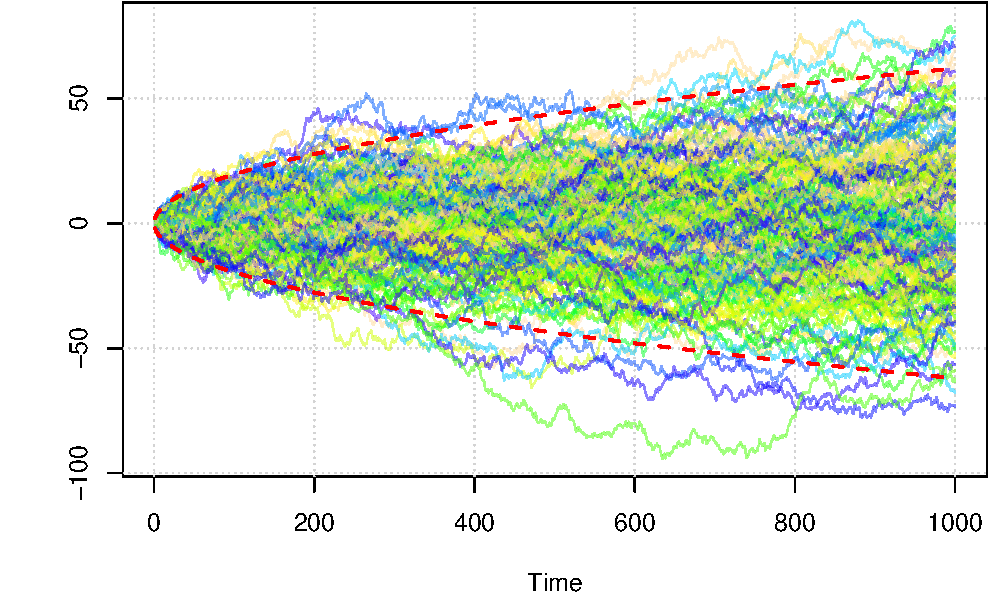
\includegraphics{ts_files/figure-latex/RWsim-1} 

}

\caption{Two hundred simulated random walks.}\label{fig:RWsim}
\end{figure}

In the plot above, two hundred simulated random walks are plotted along
with theoretical 95\% confidence intervals (red-dashed lines). The
relationship between time and variance can clearly be observed (i.e.~the
variance of the process increases with the time).

\BeginKnitrBlock{example}[Moving Average of Order 1]
\protect\hypertarget{exm:exma1}{}{\label{exm:exma1} \iffalse (Moving Average
of Order 1) \fi{} } Similarly to our previous examples, we attempt to
verify the stationary properties for the MA(1) model defined in the
previous chapter:

\begin{enumerate}
\def\labelenumi{\arabic{enumi}.}
\tightlist
\item
  \[ 
  \mathbb{E}\left[ {{X_t}} \right] = \mathbb{E}\left[ {{\theta_1}{W_{t - 1}} + {W_t}} \right] 
  = {\theta_1} \mathbb{E} \left[ {{W_{t - 1}}} \right] + \mathbb{E}\left[ {{W_t}} \right] 
  = 0. \]
\item
  \[\text{var} \left( {{X_t}} \right) = \theta_1^2 \text{var} \left( W_{t - 1}\right) + \text{var} \left( W_{t}\right) = \left(1 + \theta^2 \right) \sigma^2_w.\]\\
\item
  Regarding the autocovariance, we have \[\begin{aligned}
     \text{cov}\left( {{X_t},{X_{t + h}}} \right) &= \mathbb{E}\left[ {\left( {{X_t} - \mathbb{E}\left[ {{X_t}} \right]} \right)\left( {{X_{t + h}} - \mathbb{E}\left[ {{X_{t + h}}} \right]} \right)} \right] = \mathbb{E}\left[ {{X_t}{X_{t + h}}} \right] \\
     &= \mathbb{E}\left[ {\left( {{\theta}{W_{t - 1}} + {W_t}} \right)\left( {{\theta }{W_{t + h - 1}} + {W_{t + h}}} \right)} \right] \\
     &= \mathbb{E}\left[ {\theta^2{W_{t - 1}}{W_{t + h - 1}} + \theta {W_t}{W_{t + h}} + {\theta}{W_{t - 1}}{W_{t + h}} + {W_t}{W_{t + h}}} \right]. \\
     \end{aligned} \] It is easy to see that
  \(\mathbb{E}\left[ {{W_t}{W_{t + h}}} \right] = {\boldsymbol{1}_{\left\{ {h = 0} \right\}}}\sigma _w^2\)
  and therefore, we obtain
  \[\text{cov} \left( {{X_t},{X_{t + h}}} \right) = \left( {\theta^2{ \boldsymbol{1}_{\left\{ {h = 0} \right\}}} + {\theta}{\boldsymbol{1}_{\left\{ {h = 1} \right\}}} + {\theta}{\boldsymbol{1}_{\left\{ {h =  - 1} \right\}}} + {\boldsymbol{1}_{\left\{ {h = 0} \right\}}}} \right)\sigma _w^2\]
  implying the following autocovariance function:
  \[\gamma \left( h \right) = \left\{ {\begin{array}{*{20}{c}}
  {\left( {\theta^2 + 1} \right)\sigma _w^2}&{h = 0} \\ 
  {{\theta}\sigma _w^2}&{\left| h \right| = 1} \\ 
  0&{\left| h \right| > 1} 
  \end{array}} \right. .\] Therefore, an MA(1) process is weakly
  stationary since both the mean and variance are constant over time and
  its covariance function is only a function of the lag \((h)\).
  Finally, we can easily obtain the autocorrelation for this process,
  which is given by
  \[\rho \left( h \right) = \left\{ {\begin{array}{*{20}{c}}
    1&{h = 0} \\ 
    {\frac{{{\theta}\sigma _w^2}}{{\left( {\theta^2 + 1} \right)\sigma _w^2}} = \frac{{{\theta}}}{{\theta^2 + 1}}}&{\left| h \right| = 1} \\ 
    0&{\left| h \right| > 1} 
    \end{array}} \right. .\] Interestingly, we can note that
  \(|\rho(1)| \leq 0.5\).

  \EndKnitrBlock{example}
\end{enumerate}

\BeginKnitrBlock{example}[Autoregressive of Order 1]
\protect\hypertarget{exm:exar1}{}{\label{exm:exar1} \iffalse (Autoregressive
of Order 1) \fi{} } As another example, we shall verify the stationary
properties for the AR(1) model defined in the previous chapter.

Using the \emph{backsubstitution} technique, we can rearrange an AR(1)
process so that it is written in a more compact form, i.e.

\[\begin{aligned}
     {X_t} & =  {\phi }{X_{t - 1}} + {W_t} = \phi \left[ {\phi {X_{t - 2}} + {W_{t - 1}}} \right] + {W_t} 
     =  {\phi ^2}{X_{t - 2}} + \phi {W_{t - 1}} + {W_t}  \\
     &  \vdots  \\
     & =  {\phi ^k}{X_{t-k}} + \sum\limits_{j = 0}^{k - 1} {{\phi ^j}{W_{t - j}}} .
     \end{aligned} \]

By taking the limit in \(k\) (which is perfectly valid as we assume
\(t \in \mathbb{Z}\)) and assuming \(|\phi|<1\), we obtain

\[\begin{aligned}
     X_t = \mathop {\lim }\limits_{k \to \infty} \; {X_t}  =  \sum\limits_{j = 0}^{\infty} {{\phi ^j}{W_{t - j}}} 
     \end{aligned} \]

and therefore such a process can be interpreted as a linear combination
of white noise \((W_t)\) and corresponds (as we will observe later on)
to an MA(\(\infty\)). In addition, the requirement
\(\left| \phi \right| < 1\) turns out to be extremely useful as the
above formula is related to a \textbf{geometric series} which would
diverge if \(\phi \geq 1\) (for example when \(\phi = 1\) we have a
random walk). Indeed, remember that an infinite (converging) geometric
series is given by

\[\sum\limits_{k = 0}^\infty  \, a{{r^k}}  = \frac{a}{{1 - r}}, \; {\text{ if }}\left| r \right| < 1.\]

The origin of this requirement comes from needing to ensure that the
characteristic polynomial solution for an AR(1) lies outside the unit
circle thereby ensuring that the process is stationary. Indeed, if
\(\phi \ge 1\), the process would not converge.

With this setup, we demonstrate how crucial this property is by
calculating each of the requirements of a stationary process.

\begin{enumerate}
\def\labelenumi{\arabic{enumi}.}
\tightlist
\item
  First, we will check if the mean is stationary. In this case, we
  choose to use limits in order to derive the expectation
  \[\begin{aligned}
   \mathbb{E}\left[ {{X_t}} \right] &= \mathop {\lim }\limits_{k \to \infty } \mathbb{E}\left[ {{\phi^k}{X_{t-k}} + \sum\limits_{j = 0}^{k - 1} {\phi^j{W_{t - j}}} } \right] \\
   &= \mathop {\lim }\limits_{k \to \infty } \, \underbrace {{\phi ^k}{\mathbb{E}[X_{t-k}]}}_{= 0} + \mathop {\lim }\limits_{k \to \infty } \, \sum\limits_{j = 0}^{k - 1} {\phi^j\underbrace {\mathbb{E}\left[ {{W_{t - j}}} \right]}_{ = 0}}
   = 0.
   \end{aligned} \] As expected, the mean is zero and, hence, the first
  criterion for weak stationarity is satisfied.
\item
  Next, we determine the variance of the process \[\begin{aligned}
   \text{var}\left( {{X_t}} \right) &= \mathop {\lim }\limits_{k \to \infty } \text{var}\left( {{\phi^k}{X_{t-k}} + \sum\limits_{j = 0}^{k - 1} {\phi^j{W_{t - j}}} } \right)
   = \mathop {\lim }\limits_{k \to \infty } \sum\limits_{j = 0}^{k - 1} {\phi ^{2j} \text{var}\left( {{W_{t - j}}} \right)}  \\
   &= \mathop {\lim }\limits_{k \to \infty } \sum\limits_{j = 0}^{k - 1} \sigma _W^2 \, {\phi ^{2j}}  =  
     \underbrace {\frac{\sigma _W^2}{{1 - {\phi ^2}}}.}_{\begin{subarray}{l} 
       {\text{Geom. Series}} 
       \end{subarray}}
   \end{aligned} \] Once again, the above result only holds because we
  are able to use the convergence of the geometric series as a result of
  \(\left| \phi \right| < 1\).
\item
  Finally, we consider the autocovariance of an AR(1). For \(h > 0\), we
  have
  \[\gamma \left( h \right) =  \text{cov}\left( {{X_t},{X_{t + h}}} \right) = \phi \text{cov}\left( {{X_t},{X_{t + h - 1}}} \right) = \phi \, \gamma \left( h-1 \right).\]
  Therefore, using the symmetry of autocovariance, we find that
  \[\gamma \left( h \right) = \phi^{|h|} \, \gamma(0).\]
\end{enumerate}

Both the mean and variance do not depend on time. In addition, the
autocovariance function can be viewed as a function that only depends on
the time lag \(h\) and, thus, the AR(1) process is weakly stationary if
\(\left| \phi \right| < 1\). Lastly, we can obtain the autocorrelation
for this process. Indeed, for \(h > 0\), we have

\[\rho \left( h \right) = \frac{{\gamma \left( h \right)}}{{\gamma \left( 0 \right)}} = \frac{{\phi \gamma \left( {h - 1} \right)}}{{\gamma \left( 0 \right)}} = \phi \rho \left( {h - 1} \right).\]

After simplifying, we obtain

\[\rho \left( h \right) = {\phi^{|h|}}.\]

Thus, the autocorrelation function for an AR(1) exhibits a
\emph{geometric decay}, meaning that as \(|\phi|\) gets smaller the
autocorrelation reaches zero at a faster rate (on the contrary, if
\(|\phi|\) is close to 1 then the decay rate is slower). This is well
illustrated in the following plots.
\EndKnitrBlock{example}

\begin{figure}

{\centering 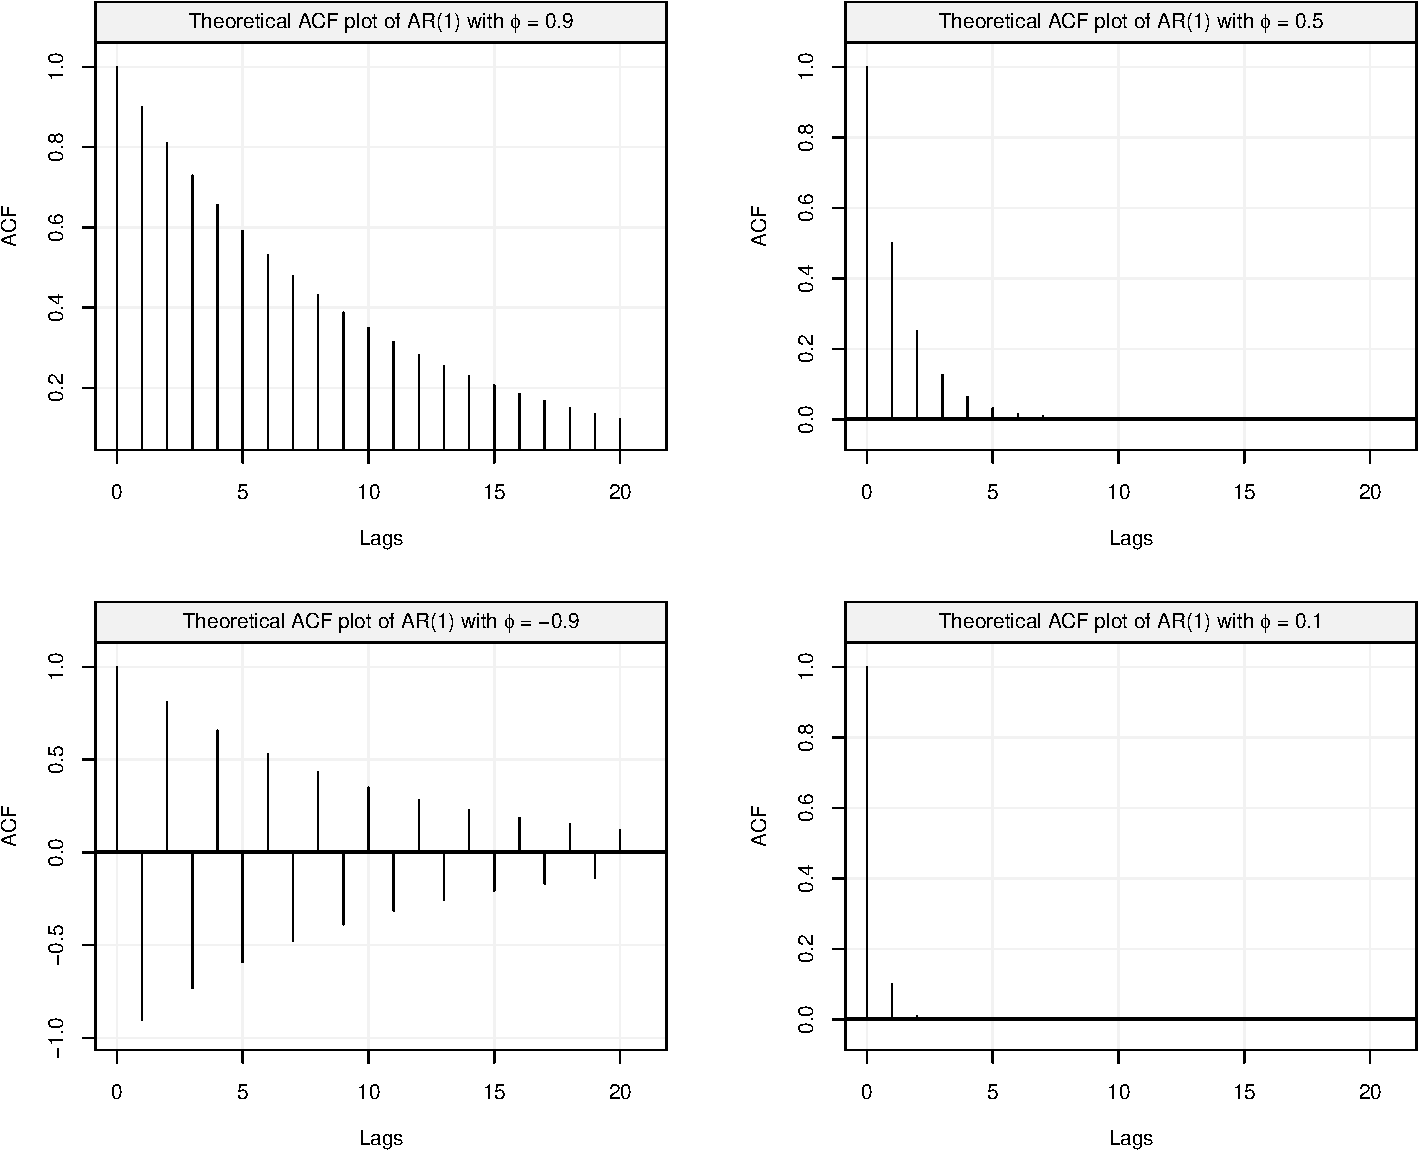
\includegraphics{ts_files/figure-latex/AR1theoACF-1} 

}

\caption{Comparison of theoretical ACF of AR(1) with different parameter values}\label{fig:AR1theoACF}
\end{figure}

\section{Estimation of Moments (Stationary
Processes)}\label{estimation-of-moments-stationary-processes}

In this section, we discuss how moments and related quantities of
stationary processes can be estimated. Informally speaking, the use of
``averages'' is meaningful for such processes suggesting that classical
moments estimators can be employed. Indeed, suppose that one is
interested in estimating \(\alpha \equiv \mathbb{E}[m (X_t)]\), where
\(m(\cdot)\) is a known function of \(X_t\). If \(X_t\) is a strongly
stationary process, we have

\[\alpha = \mathbb{E}[m(X_t) ] = \int m(x) \, f(x) dx\]

where \(f(x)\) denotes the density of \(X_t, \; \forall t\). Replacing
\(f(x)\) by \(f_n(x)\), the empirical density, we obtain the following
estimator

\[\hat{\alpha} = \widehat{\mathbb{E}}[m(X_t) ] = \frac{1}{T} \sum_{t = 1}^T m\left(x_t\right).\]

In the next subsection, we examine how this simple idea can be used to
estimate the mean, autocovariance and autocorrelation functions.
Moreover, we discuss some of the properties of these estimators.

\subsection{Estimation of the Mean
Function}\label{estimation-of-the-mean-function}

If a time series is stationary, the mean function is constant and a
possible estimator of this quantity is, as discussed above, given by

\[\bar{X} = {\frac{1}{T}\sum\limits_{t = 1}^T {{X_t}} }.\]

Naturally, the \(k\)-th moment, say \(\beta_k \equiv \mathbb{E}[X_t^k]\)
can be estimated by

\[\hat{\beta}_k = {\frac{1}{T}\sum\limits_{t = 1}^T {{X_t^k}} }, \;\; k \in \left\{x \in \mathbb{N} : \, 0 < x < \infty  \right\}.\]

The variance of such an estimator can be derived as follows:

\begin{equation}
  \begin{aligned}
  \text{var} \left( \hat{\beta}_k \right) &= \text{var} \left( {\frac{1}{T}\sum\limits_{t = 1}^T {{X_t^k}} } \right)  \\
  &= \frac{1}{{{T^2}}}\text{var} \left( {{{\left[ {\begin{array}{*{20}{c}}
    1& \cdots &1
    \end{array}} \right]}_{1 \times T}}{{\left[ {\begin{array}{*{20}{c}}
      {{X_1^k}} \\
      \vdots  \\
      {{X_n^k}}
      \end{array}} \right]}_{T \times 1}}} \right)  \\
  &= \frac{1}{{{n^2}}}{\left[ {\begin{array}{*{20}{c}}
    1& \cdots &1
    \end{array}} \right]_{1 \times T}} \, \boldsymbol{\Sigma}(k) \, {\left[ {\begin{array}{*{20}{c}}
      1 \\
      \vdots  \\
      1
      \end{array}} \right]_{T \times 1}}, 
  \end{aligned}
  \label{eq:chap2VarMoment}
\end{equation}

where \(\boldsymbol{\Sigma}(k) \in \mathbb{R}^{T \times T}\) and its
\(i\)-th, \(j\)-th element is given by

\[ \left(\boldsymbol{\Sigma}(k)\right)_{i,j} = \text{cov} \left(X_i^k, X_j^k\right).\]

In the case \(k = 1\), \eqref{eq:chap2VarMoment} can easily be further
simplified. Indeed, we have

\[\begin{aligned}
       \text{var} \left( {\bar X} \right) &= \text{var} \left( {\frac{1}{n}\sum\limits_{t = 1}^T {{X_t}} } \right)  \\
       &= \frac{1}{{{T^2}}}{\left[ {\begin{array}{*{20}{c}}
         1& \cdots &1
         \end{array}} \right]_{1 \times T}}\left[ {\begin{array}{*{20}{c}}
           {\gamma \left( 0 \right)}&{\gamma \left( 1 \right)}& \cdots &{\gamma \left( {T - 1} \right)} \\
           {\gamma \left( 1 \right)}&{\gamma \left( 0 \right)}&{}& \vdots  \\
           \vdots &{}& \ddots & \vdots  \\
           {\gamma \left( {T - 1} \right)}& \cdots & \cdots &{\gamma \left( 0 \right)}
           \end{array}} \right]_{T \times T}{\left[ {\begin{array}{*{20}{c}}
             1 \\
             \vdots  \\
             1
             \end{array}} \right]_{T \times 1}}  \\
       &= \frac{1}{{{n^2}}}\left( {T\gamma \left( 0 \right) + 2\left( {T - 1} \right)\gamma \left( 1 \right) + 2\left( {T - 2} \right)\gamma \left( 2 \right) +  \cdots  + 2\gamma \left( {T - 1} \right)} \right)  \\
       &= \frac{1}{T}\sum\limits_{h =  - T}^T {\left( {1 - \frac{{\left| h \right|}}{T}} \right)\gamma \left( h \right)} .  \\
\end{aligned} \]

Obviously, when \(X_t\) is a white noise process, the above formula
reduces to the usual
\(\text{var} \left( {\bar X} \right) = \sigma^2_w/T\). In the following
example, we consider the case of an AR(1) process and discuss how
\(\text{var} \left( {\bar X} \right)\) can be obtained or estimated.

\BeginKnitrBlock{example}
\protect\hypertarget{exm:exactvbootstrap}{}{\label{exm:exactvbootstrap} }For
an AR(1), we have
\(\gamma(h) = \phi^h \sigma_w^2 \left(1 - \phi^2\right)^{-1}\).
Therefore, we obtain (after some computations):
\EndKnitrBlock{example}

\begin{equation}
    \text{var} \left( {\bar X} \right) = \frac{\sigma_w^2 \left( T - 2\phi - T \phi^2 + 2 \phi^{T + 1}\right)}{T^2\left(1-\phi^2\right)\left(1-\phi\right)^2}.
     \label{eq:chap2exAR1}
\end{equation}

Unfortunately, deriving such an exact formula is often difficult when
considering more complex models. However, asymptotic approximations are
often employed to simplify the calculation. For example, in our case we
have

\[\mathop {\lim }\limits_{T \to \infty } \; T \text{var} \left( {\bar X} \right) = \frac{\sigma_w^2}{\left(1-\phi\right)^2},\]

providing the following approximate formula:

\[\text{var} \left( {\bar X} \right) \approx \frac{\sigma_w^2}{T \left(1-\phi\right)^2}.\]

Alternatively, simulation methods can also be employed. For example, a
possible strategy would be parametric bootstrap.

\BeginKnitrBlock{example}
\protect\hypertarget{exm:parabootstrap}{}{\label{exm:parabootstrap}
}Parametric bootstrap can be implemented in the following manner:

\begin{enumerate}
\def\labelenumi{\arabic{enumi}.}
\tightlist
\item
  Simulate a new sample under the postulated model, i.e.
  \(X_t^* \sim F_{\boldsymbol{\theta}}\) (\emph{note:} if
  \(\boldsymbol{\theta}\) is unknown it can be replaced by
  \(\hat{\boldsymbol{\theta}}\), a suitable estimator).
\item
  Compute the statistics of interest on the simulated sample
  \((X_t^*)\).
\item
  Repeat Steps 1 and 2 \(B\) times where \(B\) is sufficiently ``large''
  (typically \(100 \leq B \leq 10000\)).
\item
  Compute the empirical variance of the statistics of interest based on
  the \(B\) independent replications.

  \EndKnitrBlock{example}
\end{enumerate}

In our example, we would consider \((X_t^*)\) to be \({\bar{X}^*}\) and
seek to obtain:

\[\hat{\sigma}^2_B = \frac{1}{B-1} \sum_{i = 1}^B \left(\bar{X}^*_i - \bar{X}^* \right)^2, \;\;\; \text{where} \;\;\; \bar{X}^* = \frac{1}{B} \sum_{i=1}^B \bar{X}^*_i,\]

where \(\bar{X}^*_i\) denotes the value of the mean estimated on the
\(i\)-th simulated sample.

The figure below generated by the following code compares these three
methods for \(T = 10\), \(B = 1000,\) \(\sigma^2 = 1\) and a grid of
values for \(\phi\) going from \(-0.95\) to \(0.95\):

\begin{Shaded}
\begin{Highlighting}[]
\CommentTok{# Define sample size}
\NormalTok{n =}\StringTok{ }\DecValTok{10}

\CommentTok{# Number of Monte-Carlo replications}
\NormalTok{B =}\StringTok{ }\DecValTok{5000}

\CommentTok{# Define grid of values for phi}
\NormalTok{phi =}\StringTok{ }\KeywordTok{seq}\NormalTok{(}\DataTypeTok{from =} \FloatTok{0.95}\NormalTok{, }\DataTypeTok{to =} \OperatorTok{-}\FloatTok{0.95}\NormalTok{, }\DataTypeTok{length.out =} \DecValTok{30}\NormalTok{)}

\CommentTok{# Define result matrix}
\NormalTok{result =}\StringTok{ }\KeywordTok{matrix}\NormalTok{(}\OtherTok{NA}\NormalTok{,B,}\KeywordTok{length}\NormalTok{(phi))}

\CommentTok{# Start simulation}
\ControlFlowTok{for}\NormalTok{ (i }\ControlFlowTok{in} \KeywordTok{seq_along}\NormalTok{(phi))\{}
  \CommentTok{# Define model}
\NormalTok{  model =}\StringTok{ }\KeywordTok{AR1}\NormalTok{(}\DataTypeTok{phi =}\NormalTok{ phi[i], }\DataTypeTok{sigma2 =} \DecValTok{1}\NormalTok{)}
  
  \CommentTok{# Monte-Carlo}
  \ControlFlowTok{for}\NormalTok{ (j }\ControlFlowTok{in} \KeywordTok{seq_len}\NormalTok{(B))\{}
    \CommentTok{# Simulate AR(1)}
\NormalTok{    Xt =}\StringTok{ }\KeywordTok{gen_gts}\NormalTok{(n, model)}
    
    \CommentTok{# Estimate Xbar}
\NormalTok{    result[j,i] =}\StringTok{ }\KeywordTok{mean}\NormalTok{(Xt)}
\NormalTok{  \}}
\NormalTok{\}}

\CommentTok{# Estimate variance of Xbar}
\NormalTok{var.Xbar =}\StringTok{ }\KeywordTok{apply}\NormalTok{(result,}\DecValTok{2}\NormalTok{,var)}

\CommentTok{# Compute theoretical variance}
\NormalTok{var.theo =}\StringTok{ }\NormalTok{(n }\OperatorTok{-}\StringTok{ }\DecValTok{2}\OperatorTok{*}\NormalTok{phi }\OperatorTok{-}\StringTok{ }\NormalTok{n}\OperatorTok{*}\NormalTok{phi}\OperatorTok{^}\DecValTok{2} \OperatorTok{+}\StringTok{ }\DecValTok{2}\OperatorTok{*}\NormalTok{phi}\OperatorTok{^}\NormalTok{(n}\OperatorTok{+}\DecValTok{1}\NormalTok{))}\OperatorTok{/}\NormalTok{(n}\OperatorTok{^}\DecValTok{2}\OperatorTok{*}\NormalTok{(}\DecValTok{1}\OperatorTok{-}\NormalTok{phi}\OperatorTok{^}\DecValTok{2}\NormalTok{)}\OperatorTok{*}\NormalTok{(}\DecValTok{1}\OperatorTok{-}\NormalTok{phi)}\OperatorTok{^}\DecValTok{2}\NormalTok{)}

\CommentTok{# Compute (approximate) variance}
\NormalTok{var.approx =}\StringTok{ }\DecValTok{1}\OperatorTok{/}\NormalTok{(n}\OperatorTok{*}\NormalTok{(}\DecValTok{1}\OperatorTok{-}\NormalTok{phi)}\OperatorTok{^}\DecValTok{2}\NormalTok{)}

\CommentTok{# Compare variance estimations}
\KeywordTok{plot}\NormalTok{(}\OtherTok{NA}\NormalTok{, }\DataTypeTok{xlim =} \KeywordTok{c}\NormalTok{(}\OperatorTok{-}\DecValTok{1}\NormalTok{,}\DecValTok{1}\NormalTok{), }\DataTypeTok{ylim =} \KeywordTok{range}\NormalTok{(var.approx), }\DataTypeTok{log =} \StringTok{"y"}\NormalTok{, }
     \DataTypeTok{ylab =} \KeywordTok{expression}\NormalTok{(}\KeywordTok{paste}\NormalTok{(}\StringTok{"var("}\NormalTok{, }\KeywordTok{bar}\NormalTok{(X), }\StringTok{")"}\NormalTok{)),}
     \DataTypeTok{xlab=} \KeywordTok{expression}\NormalTok{(phi), }\DataTypeTok{cex.lab =} \DecValTok{1}\NormalTok{)}
\KeywordTok{grid}\NormalTok{()}
\KeywordTok{lines}\NormalTok{(phi,var.theo, }\DataTypeTok{col =} \StringTok{"deepskyblue4"}\NormalTok{)}
\KeywordTok{lines}\NormalTok{(phi, var.Xbar, }\DataTypeTok{col =} \StringTok{"firebrick3"}\NormalTok{)}
\KeywordTok{lines}\NormalTok{(phi,var.approx, }\DataTypeTok{col =} \StringTok{"springgreen4"}\NormalTok{)}
\KeywordTok{legend}\NormalTok{(}\StringTok{"topleft"}\NormalTok{,}\KeywordTok{c}\NormalTok{(}\StringTok{"Theoretical variance"}\NormalTok{,}\StringTok{"Bootstrap variance"}\NormalTok{,}\StringTok{"Approximate variance"}\NormalTok{), }
       \DataTypeTok{col =} \KeywordTok{c}\NormalTok{(}\StringTok{"deepskyblue4"}\NormalTok{,}\StringTok{"firebrick3"}\NormalTok{,}\StringTok{"springgreen4"}\NormalTok{), }\DataTypeTok{lty =} \DecValTok{1}\NormalTok{,}
       \DataTypeTok{bty =} \StringTok{"n"}\NormalTok{,}\DataTypeTok{bg =} \StringTok{"white"}\NormalTok{, }\DataTypeTok{box.col =} \StringTok{"white"}\NormalTok{, }\DataTypeTok{cex =} \FloatTok{1.2}\NormalTok{)}
\end{Highlighting}
\end{Shaded}

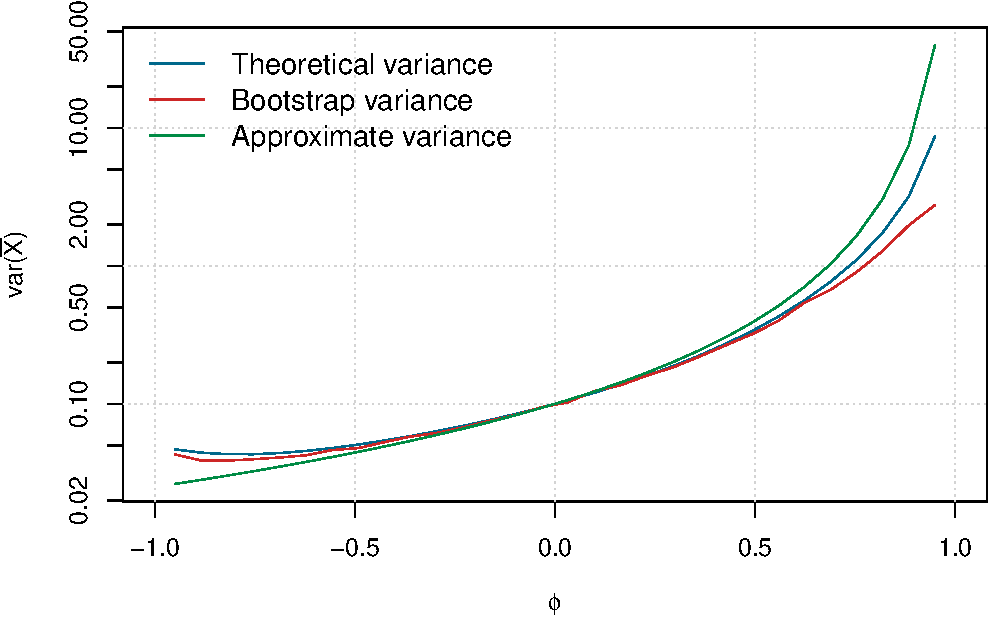
\includegraphics{ts_files/figure-latex/estimXbar-1.pdf}

It can be observed that the variance of \(\bar{X}\) typically increases
with \(\phi\). As expected when \(\phi = 0\), we have
\(\text{var}(\bar{X}) = 1/n\) and in this case the process is a white
noise. Moreover, the bootstrap approach appears to well approximate the
curve of \eqref{eq:chap2exAR1}, while the asymptotic form provides a
reasonable approximation when \(\phi\) lies between -0.5 and 0.5.
Naturally, the quality of this approximation would be far better for a
larger sample size (here we consider \(T = 10\), which is a little
``extreme'').

\subsection{Sample Autocovariance and Autocorrelation
Functions}\label{sample-autocovariance-and-autocorrelation-functions}

A natural estimator of the \emph{autocovariance function} is given by:

\[\hat \gamma \left( h \right) = \frac{1}{T}\sum\limits_{t = 1}^{T - h} {\left( {{X_t} - \bar X} \right)\left( {{X_{t + h}} - \bar X} \right)} \]

leading to the following ``plug-in'' estimator of the
\emph{autocorrelation function}:

\[\hat \rho \left( h \right) = \frac{{\hat \gamma \left( h \right)}}{{\hat \gamma \left( 0 \right)}}.\]

A graphical representation of the autocorrelation function is often the
first step for any time series analysis (again assuming the process to
be stationary). Consider the following simulated example:

\begin{Shaded}
\begin{Highlighting}[]
\CommentTok{# Set seed for reproducibility}
\KeywordTok{set.seed}\NormalTok{(}\DecValTok{2241}\NormalTok{)}

\CommentTok{# Simulate 100 observation from a Gaussian white noise}
\NormalTok{Xt =}\StringTok{ }\KeywordTok{gen_gts}\NormalTok{(}\DecValTok{100}\NormalTok{, }\KeywordTok{WN}\NormalTok{(}\DataTypeTok{sigma2 =} \DecValTok{1}\NormalTok{))}

\CommentTok{# Compute autocorrelation}
\NormalTok{acf_Xt =}\StringTok{ }\NormalTok{simts}\OperatorTok{::}\KeywordTok{auto_corr}\NormalTok{(Xt)}

\CommentTok{# Plot autocorrelation}
\KeywordTok{plot}\NormalTok{(acf_Xt, }\DataTypeTok{show.ci =} \OtherTok{FALSE}\NormalTok{)}
\end{Highlighting}
\end{Shaded}

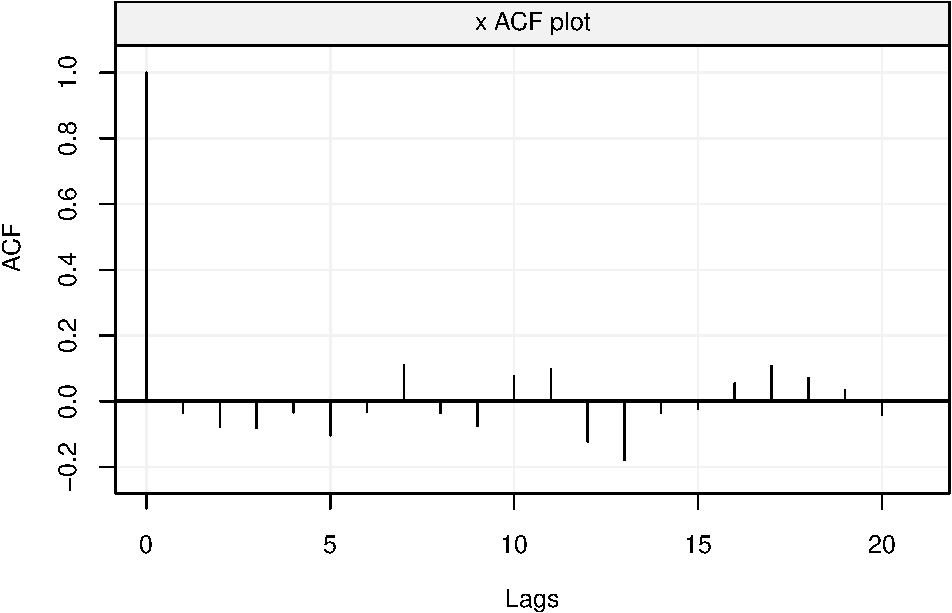
\includegraphics{ts_files/figure-latex/basicACF-1.pdf}

In this example, the true autocorrelation is equal to zero at any lag
\(h \neq 0\), but obviously the estimated autocorrelations are random
variables and are not equal to their true values. It would therefore be
useful to have some knowledge about the variability of the sample
autocorrelations (under some conditions) to assess whether the data
comes from a completely random series or presents some significant
correlation at certain lags. The following result provides an asymptotic
solution to this problem:

\BeginKnitrBlock{theorem}
\protect\hypertarget{thm:approxnormal}{}{\label{thm:approxnormal} }If
\(X_t\) is a strong white noise with finite fourth moment, then for all
\(h \in \mathbb{Z} \setminus {0}\), \(\hat{\rho}(h)\) is approximately
normally distributed with mean \(0\) and variance \(T^{-1}\).
\EndKnitrBlock{theorem}

The proof of this Theorem is given in Appendix \ref{appendixa}.

Using this result, we now have an approximate method to assess whether
peaks in the sample autocorrelation are significant by determining
whether the observed peak lies outside the interval \(\pm 2/\sqrt{T}\)
(i.e.~an approximate 95\% confidence interval). Returning to our
previous example and adding confidence bands to the previous graph, we
obtain:

\begin{Shaded}
\begin{Highlighting}[]
\CommentTok{# Plot autocorrelation with confidence bands }
\KeywordTok{plot}\NormalTok{(acf_Xt)}
\end{Highlighting}
\end{Shaded}

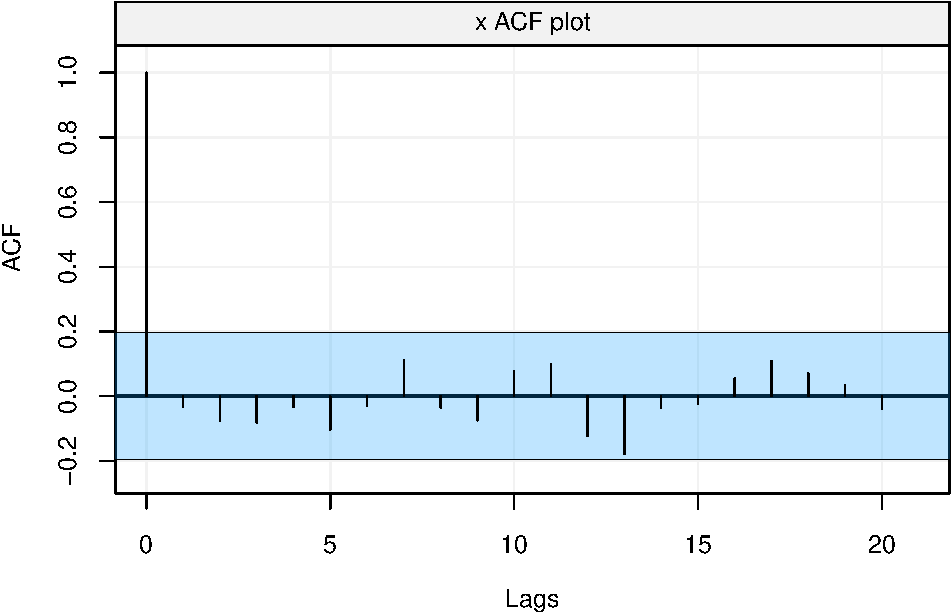
\includegraphics{ts_files/figure-latex/basicACF2-1.pdf}

It can now be observed that most peaks lie within the interval
\(\pm 2/\sqrt{T}\) suggesting that the true data generating process is
uncorrelated.

\BeginKnitrBlock{example}
\protect\hypertarget{exm:acffeatures}{}{\label{exm:acffeatures} }To
illustrate how the autocorrelation function can be used to reveal some
``features'' of a time series, we download the level of the Standard \&
Poor's 500 index, often abbreviated as the S\&P 500. This financial
index is based on the market capitalization of 500 large companies
having common stock listed on the New York Stock Exchange or the NASDAQ
Stock Market. The graph below shows the index level and daily returns
from 1990.
\EndKnitrBlock{example}

\begin{Shaded}
\begin{Highlighting}[]
\CommentTok{# Load package}
\KeywordTok{library}\NormalTok{(quantmod)}

\CommentTok{# Download S&P index}
\KeywordTok{getSymbols}\NormalTok{(}\StringTok{"^GSPC"}\NormalTok{, }\DataTypeTok{from=}\StringTok{"1990-01-01"}\NormalTok{, }\DataTypeTok{to =} \KeywordTok{Sys.Date}\NormalTok{())}
\end{Highlighting}
\end{Shaded}

\begin{verbatim}
## [1] "GSPC"
\end{verbatim}

\begin{Shaded}
\begin{Highlighting}[]
\CommentTok{# Extract index level and daily returns from the data}
\NormalTok{GSPC_index =}\StringTok{ }\KeywordTok{gts}\NormalTok{(}\DataTypeTok{data =} \KeywordTok{as.numeric}\NormalTok{(GSPC}\OperatorTok{$}\NormalTok{GSPC.Close),}
                 \DataTypeTok{start =} \DecValTok{1990}\NormalTok{,}
                 \DataTypeTok{freq =} \DecValTok{252}\NormalTok{,}
                 \DataTypeTok{Time =} \KeywordTok{time}\NormalTok{(GSPC),}
                 \DataTypeTok{unit_time =} \StringTok{"year"}\NormalTok{,}
                 \DataTypeTok{name_ts =} \StringTok{"Index Level"}\NormalTok{,}
                 \DataTypeTok{data_name =} \KeywordTok{paste}\NormalTok{(}\StringTok{"S&P 500 (1990-01-01 - "}\NormalTok{,}\KeywordTok{Sys.Date}\NormalTok{(),}\StringTok{")"}\NormalTok{, }\DataTypeTok{sep =} \StringTok{""}\NormalTok{)}
\NormalTok{                 )}

\NormalTok{GSPC_returns =}\StringTok{ }\KeywordTok{gts}\NormalTok{(}\DataTypeTok{data =} \KeywordTok{as.numeric}\NormalTok{(}\KeywordTok{ClCl}\NormalTok{(GSPC)),}
                   \DataTypeTok{start =} \DecValTok{1990}\NormalTok{,}
                   \DataTypeTok{freq =} \DecValTok{252}\NormalTok{,}
                   \DataTypeTok{Time =} \KeywordTok{time}\NormalTok{(GSPC),}
                   \DataTypeTok{unit_time =} \StringTok{"year"}\NormalTok{,}
                   \DataTypeTok{name_ts =} \StringTok{"Daily Returns"}\NormalTok{,}
                   \DataTypeTok{data_name =} \KeywordTok{paste}\NormalTok{(}\StringTok{"S&P 500 (1990-01-01 - "}\NormalTok{,}\KeywordTok{Sys.Date}\NormalTok{(),}\StringTok{")"}\NormalTok{, }\DataTypeTok{sep =} \StringTok{""}\NormalTok{)}
\NormalTok{)}

\KeywordTok{par}\NormalTok{(}\DataTypeTok{mfrow =} \KeywordTok{c}\NormalTok{(}\DecValTok{1}\NormalTok{,}\DecValTok{2}\NormalTok{))}
\KeywordTok{plot}\NormalTok{(GSPC_index)}
\KeywordTok{plot}\NormalTok{(GSPC_returns)}
\end{Highlighting}
\end{Shaded}

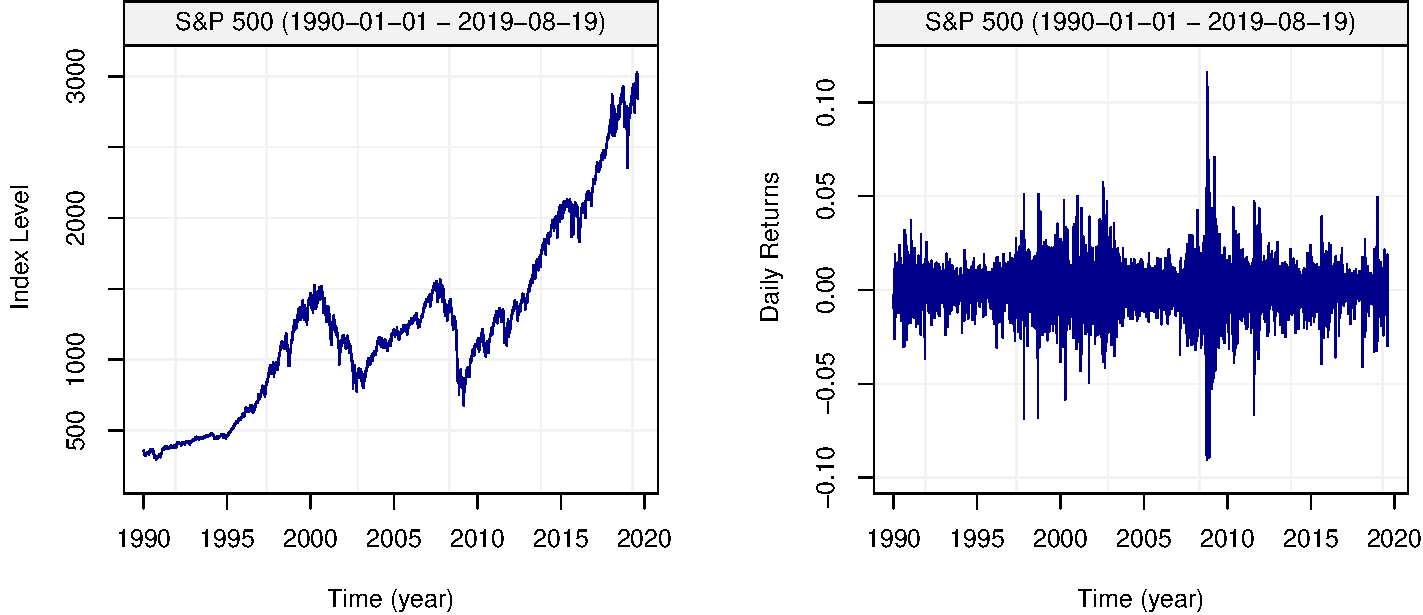
\includegraphics{ts_files/figure-latex/GSPC-1.pdf}

From these graphs, it is clear that the returns are not identically
distributed as the variance seems to change over time and clusters with
either high or low volatility can be observed. These characteristics of
financial time series are well known and further on in this book we will
discuss how the variance of such processes can be approximated.
Nevertheless, we compute the empirical autocorrelation function of the
S\&P 500 return to evaluate the degree of ``linear'' dependence between
observations. The graph below presents the empirical autocorrelation.

\begin{Shaded}
\begin{Highlighting}[]
\NormalTok{sp500 =}\StringTok{ }\KeywordTok{na.omit}\NormalTok{(GSPC_returns)}
\KeywordTok{names}\NormalTok{(sp500) =}\StringTok{ }\KeywordTok{paste}\NormalTok{(}\StringTok{"S&P 500 (1990-01-01 - "}\NormalTok{,}\KeywordTok{Sys.Date}\NormalTok{(),}\StringTok{")"}\NormalTok{, }\DataTypeTok{sep =} \StringTok{""}\NormalTok{)}
\KeywordTok{plot}\NormalTok{(simts}\OperatorTok{::}\KeywordTok{auto_corr}\NormalTok{(sp500))}
\end{Highlighting}
\end{Shaded}

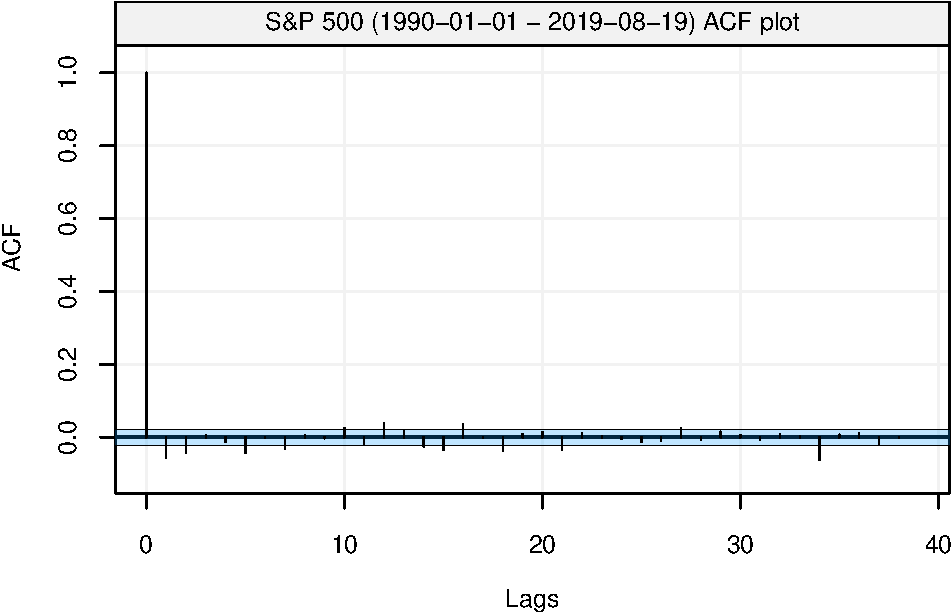
\includegraphics{ts_files/figure-latex/GSPCacf-1.pdf}

As expected, the autocorrelation is small but it might be reasonable to
believe that this sequence is not purely uncorrelated. Unfortunately,
Theorem \ref{thm:approxnormal} is based on an asymptotic argument and
since the confidence bands constructed are also asymptotic, there are no
``exact'' tools that can be used in this case. To study the validity of
these results when \(T\) is ``small'' we can perform a simulation study.
In the latter, we simulate processes from a Gaussian white noise and
examine the empirical distribution of \(\hat{\rho}(3)\) with different
sample sizes (i.e. \(n\) is set to 5, 10, 30 and 300). Intuitively, the
``quality'' of the approximation provided by Theorem
\ref{thm:approxnormal} should increase with the sample size \(T\). The
code below performs such a simulation and compares the empirical
distribution of \(\sqrt{T} \hat{\rho}(3)\) with a normal distribution
with mean 0 and variance 1 (its asymptotic distribution), which is
depicted using a red line.

\begin{Shaded}
\begin{Highlighting}[]
\CommentTok{# Number of Monte Carlo replications}
\NormalTok{B =}\StringTok{ }\DecValTok{10000}

\CommentTok{# Define considered lag}
\NormalTok{h =}\StringTok{ }\DecValTok{3}

\CommentTok{# Sample size considered}
\NormalTok{N =}\StringTok{ }\KeywordTok{c}\NormalTok{(}\DecValTok{5}\NormalTok{, }\DecValTok{10}\NormalTok{, }\DecValTok{30}\NormalTok{, }\DecValTok{300}\NormalTok{)}

\CommentTok{# Initialisation}
\NormalTok{result =}\StringTok{ }\KeywordTok{matrix}\NormalTok{(}\OtherTok{NA}\NormalTok{,B,}\KeywordTok{length}\NormalTok{(N))}

\CommentTok{# Set seed}
\KeywordTok{set.seed}\NormalTok{(}\DecValTok{1}\NormalTok{)}

\CommentTok{# Start Monte Carlo}
\ControlFlowTok{for}\NormalTok{ (i }\ControlFlowTok{in} \KeywordTok{seq_len}\NormalTok{(B))\{}
  \ControlFlowTok{for}\NormalTok{ (j }\ControlFlowTok{in} \KeywordTok{seq_along}\NormalTok{(N))\{}
    \CommentTok{# Simluate process}
\NormalTok{    Xt =}\StringTok{ }\KeywordTok{rnorm}\NormalTok{(N[j])}
    
    \CommentTok{# Save autocorrelation at lag h}
\NormalTok{    result[i,j] =}\StringTok{ }\KeywordTok{acf}\NormalTok{(Xt, }\DataTypeTok{plot =} \OtherTok{FALSE}\NormalTok{)}\OperatorTok{$}\NormalTok{acf[h}\OperatorTok{+}\DecValTok{1}\NormalTok{]}
\NormalTok{  \}}
\NormalTok{\}}

\CommentTok{# Plot results}
\KeywordTok{par}\NormalTok{(}\DataTypeTok{mfrow =} \KeywordTok{c}\NormalTok{(}\DecValTok{2}\NormalTok{,}\KeywordTok{length}\NormalTok{(N)}\OperatorTok{/}\DecValTok{2}\NormalTok{))}
\ControlFlowTok{for}\NormalTok{ (i }\ControlFlowTok{in} \KeywordTok{seq_along}\NormalTok{(N))\{}
  \CommentTok{# Estimated empirical distribution}
  \KeywordTok{hist}\NormalTok{(}\KeywordTok{sqrt}\NormalTok{(N[i])}\OperatorTok{*}\NormalTok{result[,i], }\DataTypeTok{col =} \StringTok{"royalblue1"}\NormalTok{, }
       \DataTypeTok{main =} \KeywordTok{paste}\NormalTok{(}\StringTok{"Sample size n ="}\NormalTok{,N[i]), }\DataTypeTok{probability =} \OtherTok{TRUE}\NormalTok{,}
       \DataTypeTok{xlim =} \KeywordTok{c}\NormalTok{(}\OperatorTok{-}\DecValTok{4}\NormalTok{,}\DecValTok{4}\NormalTok{), }\DataTypeTok{xlab =} \StringTok{" "}\NormalTok{)}
  
  \CommentTok{# Asymptotic distribution}
\NormalTok{  xx =}\StringTok{ }\KeywordTok{seq}\NormalTok{(}\DataTypeTok{from =} \OperatorTok{-}\DecValTok{10}\NormalTok{, }\DataTypeTok{to =} \DecValTok{10}\NormalTok{, }\DataTypeTok{length.out =} \DecValTok{10}\OperatorTok{^}\DecValTok{3}\NormalTok{)}
\NormalTok{  yy =}\StringTok{ }\KeywordTok{dnorm}\NormalTok{(xx,}\DecValTok{0}\NormalTok{,}\DecValTok{1}\NormalTok{)}
  \KeywordTok{lines}\NormalTok{(xx,yy, }\DataTypeTok{col =} \StringTok{"red"}\NormalTok{, }\DataTypeTok{lwd =} \DecValTok{2}\NormalTok{)}
\NormalTok{\}}
\end{Highlighting}
\end{Shaded}

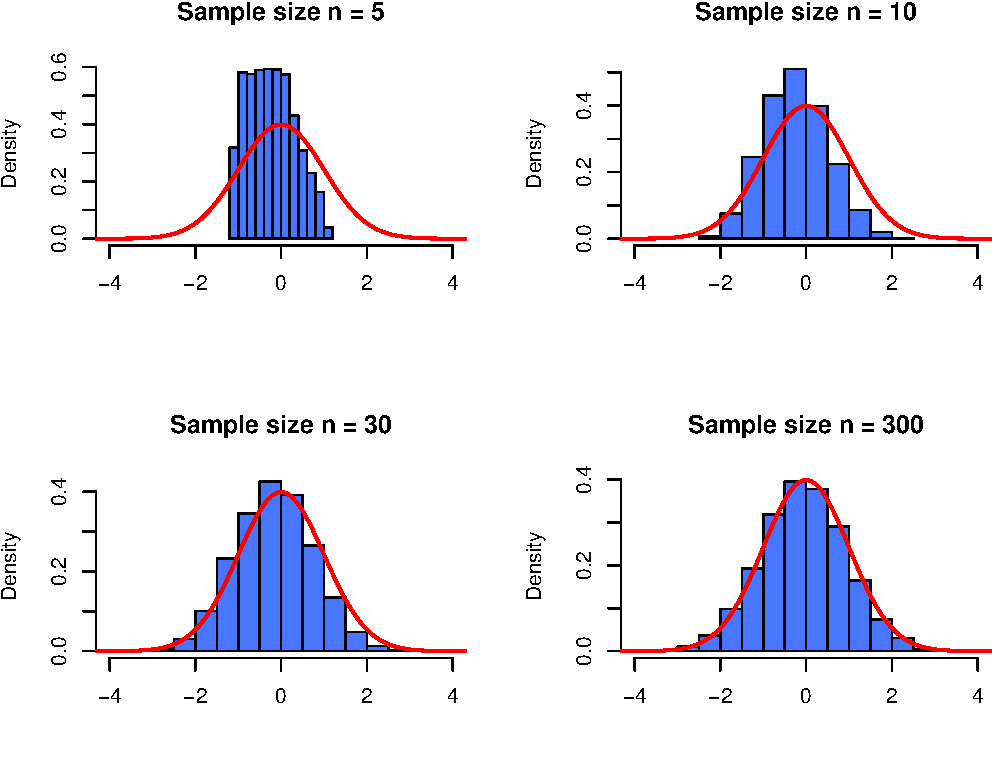
\includegraphics{ts_files/figure-latex/simulationACF-1.pdf}

As expected, it can clearly be observed that the asymptotic
approximation is quite poor when \(n = 5\) but as the sample size
increases the approximation improves and is very close when, for
example, \(T = 300\). Therefore, this simulation would suggest that
Theorem \ref{thm:approxnormal} provides a relatively ``close''
approximation of the distribution of \(\hat{\rho}(h)\), especially when
the sample size is large enough.

\subsection{Robustness Issues}\label{robustness-issues}

The data generating process delivers a theoretical autocorrelation
(autocovariance) function that, as explained in the previous section,
can then be estimated through the sample autocorrelation
(autocovariance) functions. However, in practice, the sample is often
issued from a data generating process that is ``close'' to the true one,
meaning that the sample suffers from some form of small contamination.
This contamination is typically represented by a small amount of extreme
observations that are called ``outliers'' that come from a process that
is different from the true data generating process.

The fact that the sample can suffer from outliers implies that the
standard estimation of the autocorrelation (autocovariance) functions
through the sample functions could be highly biased. The standard
estimators presented in the previous section are therefore not
``robust'' and can behave badly when the sample suffers from
contamination. To illustrate this limitation for a classical estimator,
we consider the following two processes:

\[ 
    \begin{aligned}
    X_t &= \phi X_{t-1} + W_t, \;\;\; W_t \sim \mathcal{N}(0,\sigma_w^2),\\
    Y_t &= \begin{cases}
    X_t       & \quad \text{with probability } 1 - \epsilon\\
    U_t  & \quad \text{with probability } \epsilon\\
    \end{cases}, \;\;\; U_t \sim \mathcal{N}(0,\sigma_u^2),
    \end{aligned}
\]

where \(\epsilon\) is ``small'' and \(\sigma_u^2 \gg \sigma_w^2\). The
process \((Y_t)\) can be interpreted as a ``contaminated'' version of
\((X_t)\) and the figure below represents one realization of the process
\((Y_t)\) using the following setting: \(T = 100\), \(\sigma_u^2 = 10\),
\(\phi = 0.9\), \(\sigma_w^2 = 1\) as well as \(\alpha = 0.05\).

\begin{Shaded}
\begin{Highlighting}[]
\CommentTok{# Set seed for reproducibility}
\KeywordTok{set.seed}\NormalTok{(}\DecValTok{2241}\NormalTok{)}

\CommentTok{# Define length of time series}
\NormalTok{N =}\StringTok{ }\DecValTok{100}

\CommentTok{# Select observations from contamination distribution}
\NormalTok{epsilon =}\StringTok{ }\FloatTok{0.05}
\NormalTok{index =}\StringTok{ }\KeywordTok{sample}\NormalTok{(}\DecValTok{1}\OperatorTok{:}\NormalTok{N, }\KeywordTok{round}\NormalTok{(epsilon}\OperatorTok{*}\NormalTok{N))}
\NormalTok{Ut =}\StringTok{ }\KeywordTok{gen_gts}\NormalTok{(N, }\KeywordTok{WN}\NormalTok{(}\DataTypeTok{sigma2 =} \DecValTok{10}\NormalTok{))}

\CommentTok{# Simulate observations from Xt and Yt}
\NormalTok{Xt =}\StringTok{ }\KeywordTok{gen_gts}\NormalTok{(N, }\KeywordTok{AR1}\NormalTok{(}\DataTypeTok{phi =} \FloatTok{0.9}\NormalTok{, }\DataTypeTok{sigma2 =} \DecValTok{1}\NormalTok{))}
\NormalTok{Yt =}\StringTok{ }\NormalTok{Xt}
\NormalTok{Yt[index] =}\StringTok{ }\NormalTok{Ut[index]}

\CommentTok{# Plot time series}
\KeywordTok{par}\NormalTok{(}\DataTypeTok{mfrow =} \KeywordTok{c}\NormalTok{(}\DecValTok{1}\NormalTok{,}\DecValTok{1}\NormalTok{))}
\KeywordTok{plot}\NormalTok{(Yt, }\DataTypeTok{main =} \StringTok{"Contaminated Time Series Yt"}\NormalTok{)}
\end{Highlighting}
\end{Shaded}

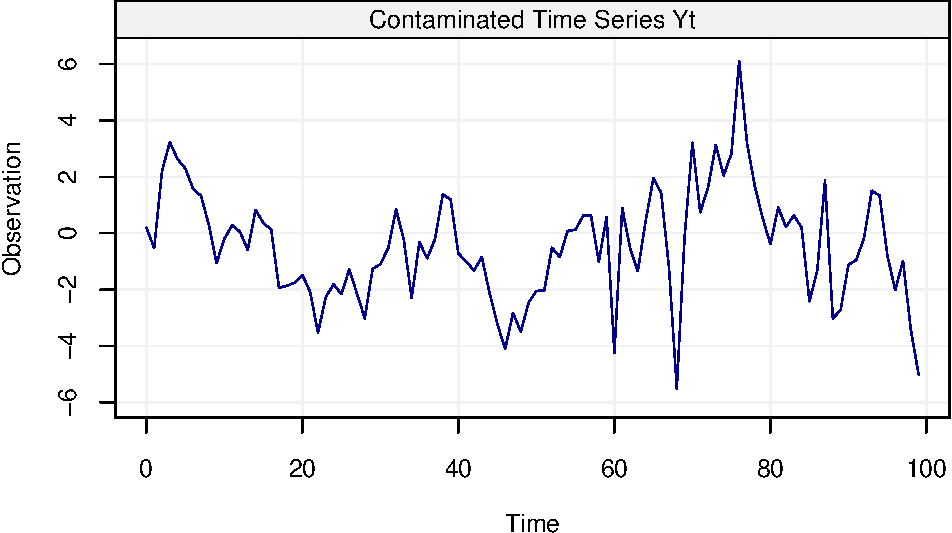
\includegraphics{ts_files/figure-latex/Yt-1.pdf}

The first question we can ask ourselves looking at this figure is: where
are the outliers? 🤔 You can probably spot a few but there are 5
outliers. If you're having difficulties detecting the outliers don't
worry: it's a commonly known phenomenon in time series that detecting
outliers is not always easy. Indeed, when looking at a time series for
the first time it's not straightforward to understand if there's any
form of contamination. Let's now compare \((X_t)\) and \((Y_t)\) in the
following plots.

\begin{Shaded}
\begin{Highlighting}[]
\CommentTok{# Plot time series}
\KeywordTok{par}\NormalTok{(}\DataTypeTok{mfrow =} \KeywordTok{c}\NormalTok{(}\DecValTok{2}\NormalTok{,}\DecValTok{1}\NormalTok{))}
\KeywordTok{plot}\NormalTok{(Xt, }\DataTypeTok{main =} \StringTok{"Original Time Series Xt"}\NormalTok{)}
\KeywordTok{plot}\NormalTok{(Yt, }\DataTypeTok{main =} \StringTok{"Contaminated Time Series Yt"}\NormalTok{)}
\KeywordTok{points}\NormalTok{(index}\OperatorTok{-}\DecValTok{1}\NormalTok{, Yt[index], }\DataTypeTok{col =} \StringTok{"red"}\NormalTok{)}
\end{Highlighting}
\end{Shaded}

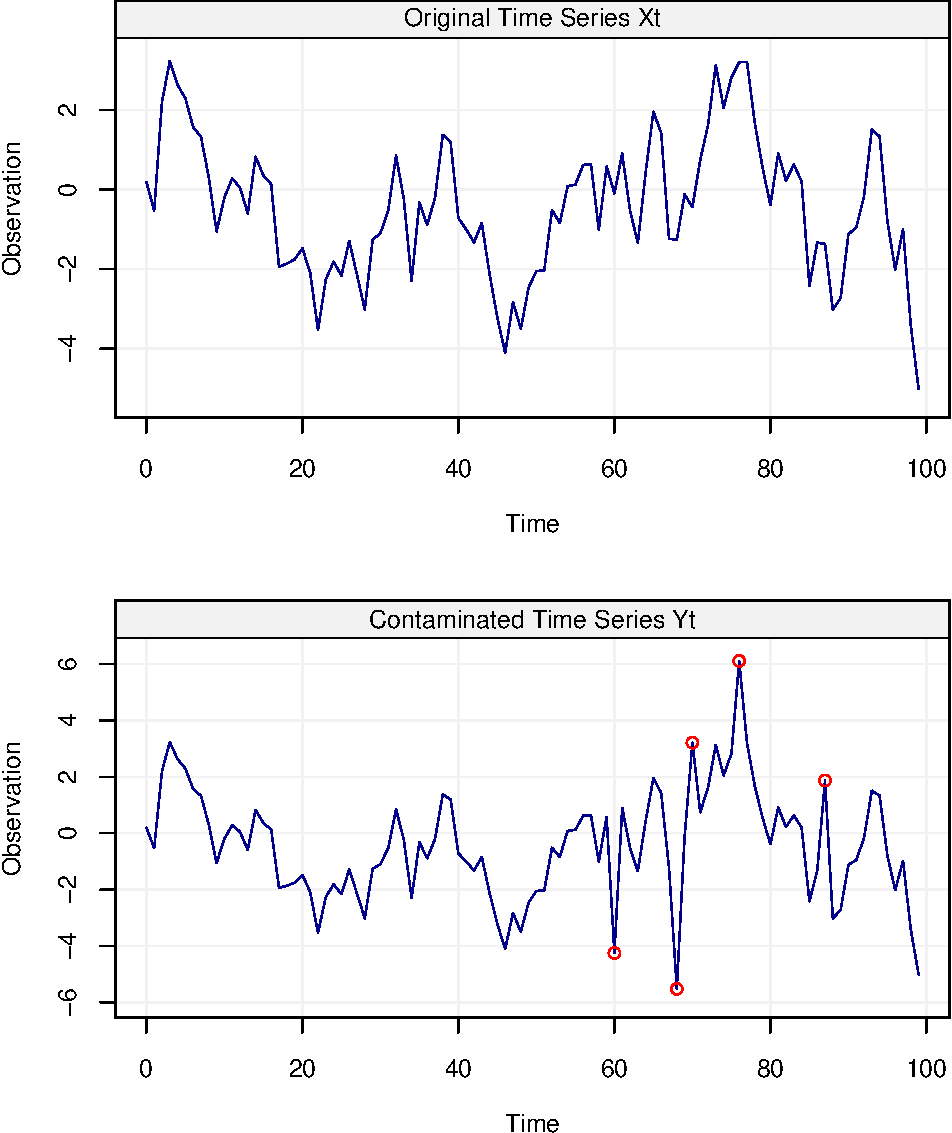
\includegraphics{ts_files/figure-latex/XtYt-1.pdf}

In this case it's more simple to detect the outliers (that are also
highlighted with the red dots) since we can compare \((Y_t)\) with the
original uncontaminated time series \((X_t)\). Having highlighted how
exploratory analysis can provide limited information on the presence of
contamination in an observed time series, we now consider a simulated
example to highlight how the performance of a ``classical''
autocorrelation estimator can deteriorate if the sample is contaminated
(i.e.~what is the impact of \((Y_t)\) on the ACF estimator
\(\hat{\rho}(h)\)). In this simulation, we will use the setting
presented above and consider \(B = 10^3\) bootstrap replications
comparing the performance of the classical estimator when applied to an
uncontaminated time series \((X_t)\) and a contaminated time series
\((Y_t)\).

\begin{Shaded}
\begin{Highlighting}[]
\NormalTok{B =}\StringTok{ }\DecValTok{1000} \CommentTok{# Number of simulations}
\NormalTok{N =}\StringTok{ }\DecValTok{100} \CommentTok{# Length of time series}
\NormalTok{epsilon =}\StringTok{ }\FloatTok{0.05} \CommentTok{# Amount of contamination}
\NormalTok{phi =}\StringTok{ }\FloatTok{0.9} \CommentTok{# AR(1) parameter value}

\CommentTok{# Store first 15 values of Empirical ACF (for Xt and Yt)}
\NormalTok{acf_xt =}\StringTok{ }\NormalTok{acf_yt =}\StringTok{ }\KeywordTok{matrix}\NormalTok{(}\OtherTok{NA}\NormalTok{, B, }\DecValTok{15}\NormalTok{)}

\ControlFlowTok{for}\NormalTok{(i }\ControlFlowTok{in} \DecValTok{1}\OperatorTok{:}\NormalTok{B) \{}
  
  \CommentTok{# Set seed for reproducibility}
  \KeywordTok{set.seed}\NormalTok{(i }\OperatorTok{+}\StringTok{ }\DecValTok{2241}\NormalTok{)}

  \CommentTok{# Select observations from contamination distribution}
\NormalTok{  index =}\StringTok{ }\KeywordTok{sample}\NormalTok{(}\DecValTok{1}\OperatorTok{:}\NormalTok{N, }\KeywordTok{round}\NormalTok{(epsilon}\OperatorTok{*}\NormalTok{N))}
\NormalTok{  Ut =}\StringTok{ }\KeywordTok{gen_gts}\NormalTok{(N, }\KeywordTok{WN}\NormalTok{(}\DataTypeTok{sigma2 =} \DecValTok{10}\NormalTok{))}

  \CommentTok{# Simulate observations from Xt and Yt}
\NormalTok{  Xt =}\StringTok{ }\KeywordTok{gen_gts}\NormalTok{(N, }\KeywordTok{AR1}\NormalTok{(}\DataTypeTok{phi =} \FloatTok{0.9}\NormalTok{, }\DataTypeTok{sigma2 =} \DecValTok{1}\NormalTok{))}
\NormalTok{  Yt =}\StringTok{ }\NormalTok{Xt}
\NormalTok{  Yt[index] =}\StringTok{ }\NormalTok{Ut[index]}
  
  \CommentTok{# Store ACF values}
\NormalTok{  acf_xt[i, ] =}\StringTok{ }\KeywordTok{as.numeric}\NormalTok{(}\KeywordTok{auto_corr}\NormalTok{(Xt))[}\DecValTok{1}\OperatorTok{:}\DecValTok{15}\NormalTok{]}
\NormalTok{  acf_yt[i, ] =}\StringTok{ }\KeywordTok{as.numeric}\NormalTok{(}\KeywordTok{auto_corr}\NormalTok{(Yt))[}\DecValTok{1}\OperatorTok{:}\DecValTok{15}\NormalTok{]}
  
\NormalTok{\}}

\CommentTok{# Compute the Theoretical ACF of an AR(1) model (up to lag 15)}
\NormalTok{true_acf =}\StringTok{ }\NormalTok{phi}\OperatorTok{^}\NormalTok{(}\DecValTok{1}\OperatorTok{:}\DecValTok{15}\NormalTok{)}

\CommentTok{# Make boxplots of Empirical ACF for both settings and compare with true ACF}
\KeywordTok{par}\NormalTok{(}\DataTypeTok{mfrow =} \KeywordTok{c}\NormalTok{(}\DecValTok{1}\NormalTok{,}\DecValTok{2}\NormalTok{))}
\KeywordTok{boxplot}\NormalTok{(acf_xt[, }\DecValTok{3}\NormalTok{], }\DataTypeTok{col =} \StringTok{"grey80"}\NormalTok{, }\DataTypeTok{main =} \StringTok{"ACF at lag 3 (uncontaminated)"}\NormalTok{)}
\KeywordTok{abline}\NormalTok{(}\DataTypeTok{h =}\NormalTok{ true_acf[}\DecValTok{3}\NormalTok{], }\DataTypeTok{col =} \StringTok{"red"}\NormalTok{)}
\KeywordTok{boxplot}\NormalTok{(acf_yt[, }\DecValTok{3}\NormalTok{], }\DataTypeTok{col =} \StringTok{"grey80"}\NormalTok{, }\DataTypeTok{main =} \StringTok{"ACF at lag 3 (contaminated)"}\NormalTok{)}
\KeywordTok{abline}\NormalTok{(}\DataTypeTok{h =}\NormalTok{ true_acf[}\DecValTok{3}\NormalTok{], }\DataTypeTok{col =} \StringTok{"red"}\NormalTok{)}
\end{Highlighting}
\end{Shaded}

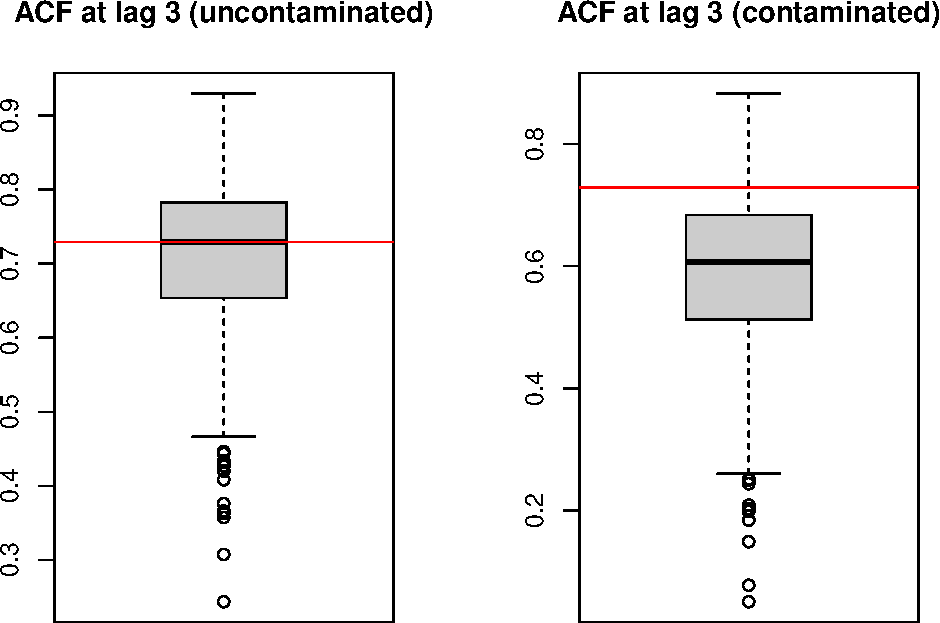
\includegraphics{ts_files/figure-latex/simulationRobust-1.pdf}

The boxplots represent the empirical distribution of the ACF estimator
\(\hat{\rho}(3)\): the left boxplot shows how the standard
autocorrelation estimator is centered around the true value (red line)
when the sample is not contaminated while the right boxplot shows how
this estimate is considerably biased when the sample is contaminated.
Indeed, it can be seen how the boxplot under contamination shows a lower
value of autocorrelation indicating that it does not detect much
dependence in the data although it should. The latter phenomenon is even
more evident when analysing the empirical distributions at the larger
lags. This is a known result in robustness, more specifically that
outliers in the data can break the dependence structure and make it more
difficult for the latter to be detected.

In order to limit this problem, different robust estimators exist for
time series problems which are designed to reduce the impact of
contamination on the estimation procedure. Among these estimators, there
are a few that estimate the autocorrelation (autocovariance) functions
in a robust manner. One of these estimators is provided in the
\texttt{robacf()} function in the ``robcor'' package. The following
simulated example shows how it limits the bias which is induced on the
classic estimator \(\hat{\rho}(h)\) from contamination. Unlike the
previous simulation, we shall only consider data issued from the
contaminated process \((Y_t)\), and compare the performance of two
estimators (i.e.~classical and robust autocorrelation estimators):

\begin{Shaded}
\begin{Highlighting}[]
\NormalTok{B =}\StringTok{ }\DecValTok{1000} \CommentTok{# Number of simulations}
\NormalTok{N =}\StringTok{ }\DecValTok{100} \CommentTok{# Length of time series}
\NormalTok{epsilon =}\StringTok{ }\FloatTok{0.05} \CommentTok{# Amount of contamination}
\NormalTok{phi =}\StringTok{ }\FloatTok{0.9} \CommentTok{# AR(1) parameter value}

\CommentTok{# Store first 15 values of Empirical ACF (classic and robust)}
\NormalTok{cl_acf =}\StringTok{ }\NormalTok{rob_acf =}\StringTok{ }\KeywordTok{matrix}\NormalTok{(}\OtherTok{NA}\NormalTok{, B, }\DecValTok{15}\NormalTok{)}

\ControlFlowTok{for}\NormalTok{(i }\ControlFlowTok{in} \DecValTok{1}\OperatorTok{:}\NormalTok{B) \{}
  
  \CommentTok{# Set seed for reproducibility}
  \KeywordTok{set.seed}\NormalTok{(i }\OperatorTok{+}\StringTok{ }\DecValTok{2241}\NormalTok{)}

  \CommentTok{# Select observations from contamination distribution}
\NormalTok{  index =}\StringTok{ }\KeywordTok{sample}\NormalTok{(}\DecValTok{1}\OperatorTok{:}\NormalTok{N, }\KeywordTok{round}\NormalTok{(epsilon}\OperatorTok{*}\NormalTok{N))}
\NormalTok{  Ut =}\StringTok{ }\KeywordTok{gen_gts}\NormalTok{(N, }\KeywordTok{WN}\NormalTok{(}\DataTypeTok{sigma2 =} \DecValTok{10}\NormalTok{))}

  \CommentTok{# Simulate observations from  Yt}
\NormalTok{  Yt =}\StringTok{ }\KeywordTok{gen_gts}\NormalTok{(N, }\KeywordTok{AR1}\NormalTok{(}\DataTypeTok{phi =} \FloatTok{0.9}\NormalTok{, }\DataTypeTok{sigma2 =} \DecValTok{1}\NormalTok{))}
\NormalTok{  Yt[index] =}\StringTok{ }\NormalTok{Ut[index]}
  
  \CommentTok{# Store Classic and Robust ACF values}
\NormalTok{  cl_acf[i, ] =}\StringTok{ }\KeywordTok{as.numeric}\NormalTok{(}\KeywordTok{auto_corr}\NormalTok{(Yt))[}\DecValTok{1}\OperatorTok{:}\DecValTok{15}\NormalTok{]}
\NormalTok{  rob_acf[i, ] =}\StringTok{ }\KeywordTok{as.numeric}\NormalTok{(}\KeywordTok{auto_corr}\NormalTok{(Yt, }\DataTypeTok{robust =} \OtherTok{TRUE}\NormalTok{))[}\DecValTok{1}\OperatorTok{:}\DecValTok{15}\NormalTok{]}
  
\NormalTok{\}}

\CommentTok{# Compute the Theoretical ACF of an AR(1) model (up to lag 15)}
\NormalTok{true_acf =}\StringTok{ }\NormalTok{phi}\OperatorTok{^}\NormalTok{(}\DecValTok{1}\OperatorTok{:}\DecValTok{15}\NormalTok{)}

\CommentTok{# Make boxplots of both Classic and Robust Empirical ACF and compare with true ACF}
\KeywordTok{par}\NormalTok{(}\DataTypeTok{mfrow =} \KeywordTok{c}\NormalTok{(}\DecValTok{1}\NormalTok{,}\DecValTok{2}\NormalTok{))}
\KeywordTok{boxplot}\NormalTok{(cl_acf[, }\DecValTok{2}\NormalTok{], }\DataTypeTok{col =} \StringTok{"grey80"}\NormalTok{, }\DataTypeTok{main =} \StringTok{"Classic ACF at lag 2"}\NormalTok{)}
\KeywordTok{abline}\NormalTok{(}\DataTypeTok{h =}\NormalTok{ true_acf[}\DecValTok{2}\NormalTok{], }\DataTypeTok{col =} \StringTok{"red"}\NormalTok{)}
\KeywordTok{boxplot}\NormalTok{(rob_acf[, }\DecValTok{2}\NormalTok{], }\DataTypeTok{col =} \StringTok{"grey80"}\NormalTok{, }\DataTypeTok{main =} \StringTok{"Robust ACF at lag 2"}\NormalTok{)}
\KeywordTok{abline}\NormalTok{(}\DataTypeTok{h =}\NormalTok{ true_acf[}\DecValTok{2}\NormalTok{], }\DataTypeTok{col =} \StringTok{"red"}\NormalTok{)}
\end{Highlighting}
\end{Shaded}

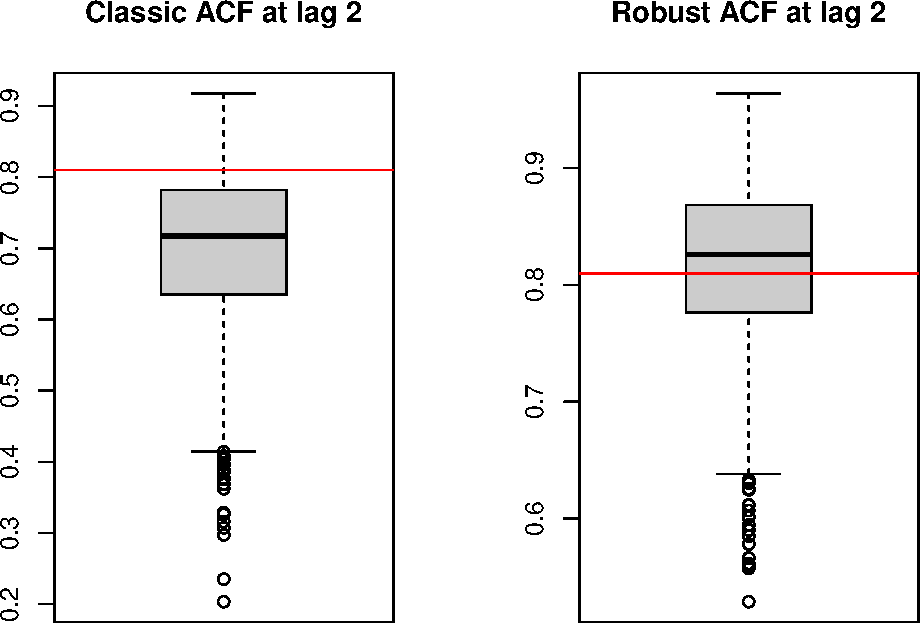
\includegraphics{ts_files/figure-latex/simulationRobust2-1.pdf}

In this case we see the empirical distributions of the two estimators
(classic and robust) for the ACF at time-lag \(h = 2\). As you can see,
the robust estimator remains close to the true value represented by the
red line in the boxplots as opposed to the standard estimator. However,
the price to pay in terms of bias reduction is a loss of efficiency of
the robust estimator. Indeed it can often be observed that to reduce the
bias induced by contamination in the sample, robust estimators pay a
certain price in terms of efficiency.

To assess how much is ``lost'' by the robust estimator compared to the
classical one in terms of efficiency, we consider one last simulation
where we examine the performance of two estimators on data issued from
the uncontaminated process, i.e. \((X_t)\). Therefore, the only
difference between this simulation and the previous one is the value of
\(\epsilon\) set equal to \(0\) (the code shall thus be omitted). For
this reason we simply show a plot that represents the ratio of the
variances of the classic and robust ACF estimators respectively. If they
happened to have the same efficiency, we would expect this ratio to be
roughly equal to 1 over all the considered lags (we omit this ratio at
lag 1 since it is numerically impossible to represent due to the
infinitesimal size of the empirical variances).

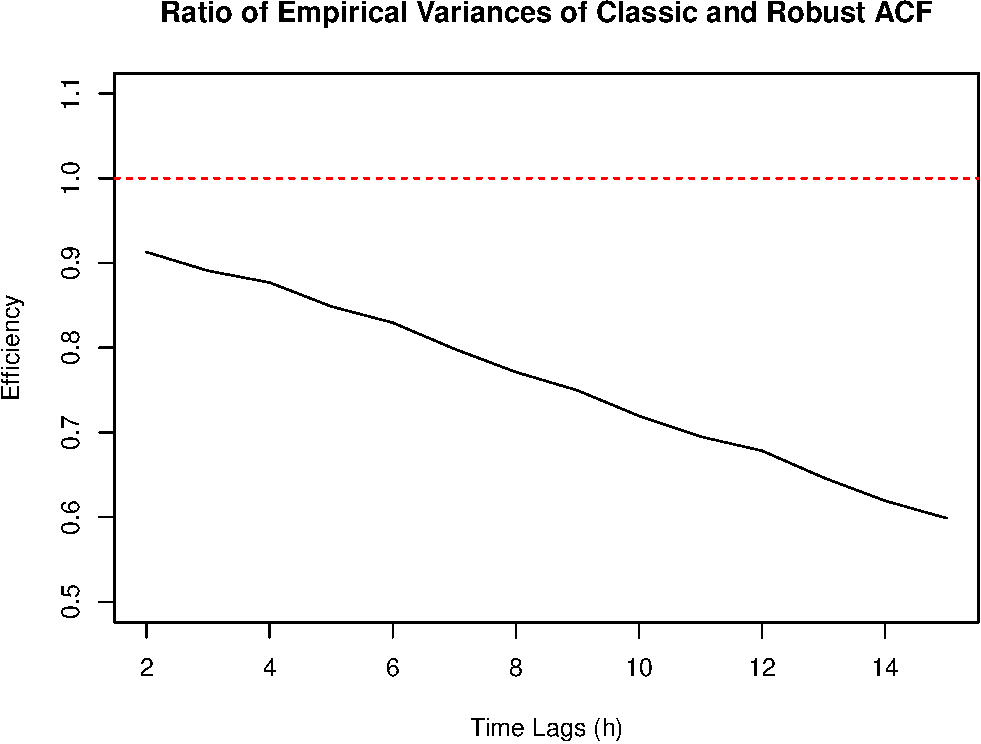
\includegraphics{ts_files/figure-latex/simulationRobust3-1.pdf}

As can be seen on the plot, the black line representing the above
described ratio decreases steadily as the lags increase and moves
further away from the red dotted line representing equality of
variances. Hence, since the variance of the classic ACF estimator is in
the numerator of this ratio, we can conclude that the variance of the
robust ACF estimator is always larger and increases over the lags. This
can partly be explained by the fact that the classic ACF estimator
\(\hat{\rho}(h)\) makes use of all the observations while the robust
estimator only uses part of the information coming from more ``extreme''
observations. Moreover, the number of observations available to estimate
the greater lags is smaller and therefore the robust ACF estimator pays
a larger price in terms of ``loss'' of information.

Let us finally investigate the importance of robust ACF estimation on
some real data. We consider the data on monthly precipitation
(\texttt{hydro}) presented in the previous chapter. This data is
measured over 65 years (between 1907 and 1972) and is an example of data
that is used to determine the behaviour of a water cycle. More
specifically, precipitation is often considered the starting point for
the analysis of a water cycle and, based on its behaviour, the rest of
the water cycle is determined based on other variables. Therefore, a
correct analysis of precipitation is extremely important to correctly
define the behaviour of the water cycle passing through run-off and
groundwater formation to evaporation and condensation. Given this, let
us now take a look at the classic autocorrelation plot of this data.

\begin{Shaded}
\begin{Highlighting}[]
\CommentTok{# Load hydro dataset}
\KeywordTok{data}\NormalTok{(}\StringTok{"hydro"}\NormalTok{)}

\CommentTok{# Define the time series as a gts object}
\NormalTok{hydro =}\StringTok{ }\KeywordTok{gts}\NormalTok{(}\KeywordTok{as.vector}\NormalTok{(hydro), }\DataTypeTok{start =} \DecValTok{1907}\NormalTok{, }\DataTypeTok{freq =} \DecValTok{12}\NormalTok{, }\DataTypeTok{unit_ts =} \StringTok{"mm"}\NormalTok{, }\DataTypeTok{name_ts =} \StringTok{"Precipitation"}\NormalTok{, }\DataTypeTok{data_name =} \StringTok{"Hydrology data"}\NormalTok{)}

\CommentTok{# Plot the Empirical ACF}
\KeywordTok{plot}\NormalTok{(}\KeywordTok{auto_corr}\NormalTok{(hydro))}
\end{Highlighting}
\end{Shaded}

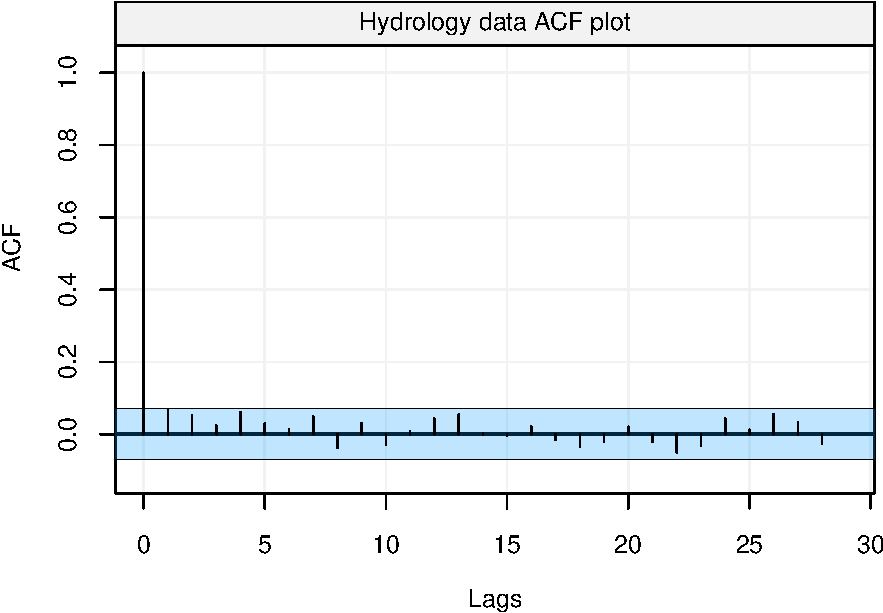
\includegraphics{ts_files/figure-latex/unnamed-chunk-23-1.pdf}

Based on this ACF plot, one would probably conclude that
(counterintuitively) there does not appear to be any significant form of
correlation between lagged observations in the data. From a hydrological
point of view, one would therefore assume an uncorrelated model for
precipitation (i.e.~white noise) and, based on this, model the rest of
the water cycle. However, let us take a look at the robust ACF plot.

\begin{Shaded}
\begin{Highlighting}[]
\CommentTok{# Plot the Robust ACF}
\KeywordTok{plot}\NormalTok{(}\KeywordTok{auto_corr}\NormalTok{(hydro, }\DataTypeTok{robust =} \OtherTok{TRUE}\NormalTok{))}
\end{Highlighting}
\end{Shaded}

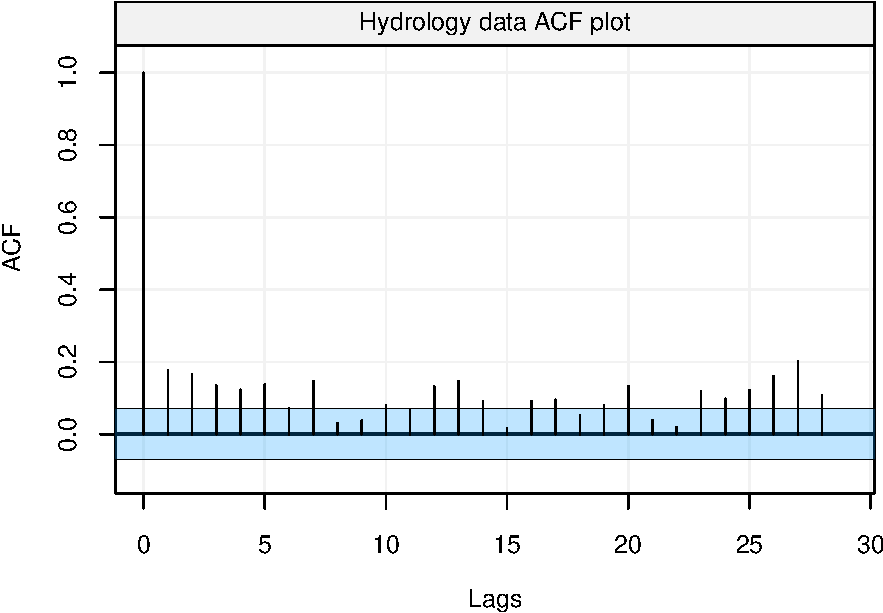
\includegraphics{ts_files/figure-latex/unnamed-chunk-24-1.pdf}

If we analyse this output, the conclusion appears to be extremely
different and, in some way, makes more sense from a hydrological point
of view (i.e.~the amount of precipitation between close months and over
specific months is correlated). Indeed, we can see that there appears to
be a seasonal correlation (``waves'' in the ACF plot) and that close
months appear to be correlated between them. To better highlight this
difference (whci can lead to different conclusions) let us finally
compare the plots.

\begin{Shaded}
\begin{Highlighting}[]
\CommentTok{# Compare classic and robust ACF}
\KeywordTok{compare_acf}\NormalTok{(hydro)}
\end{Highlighting}
\end{Shaded}

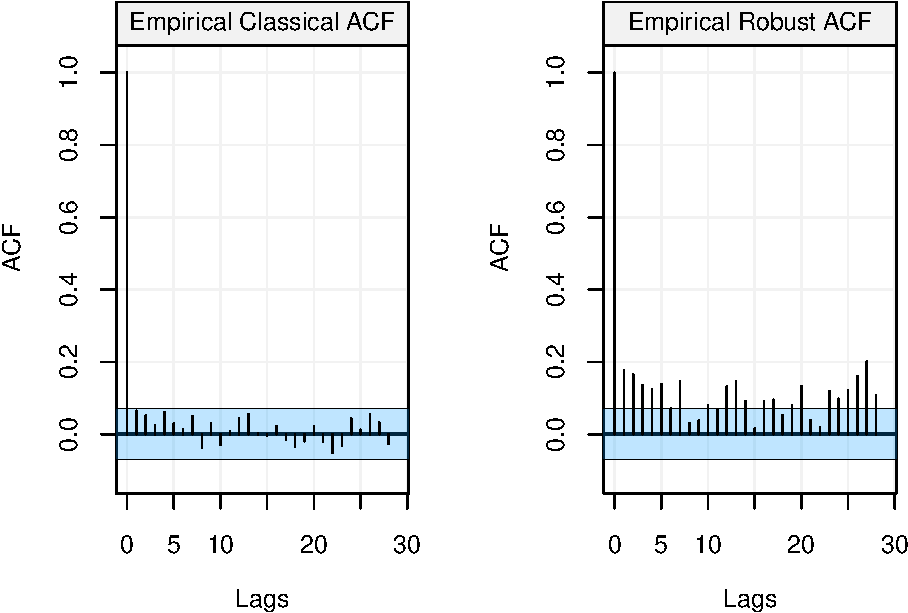
\includegraphics{ts_files/figure-latex/unnamed-chunk-25-1.pdf}

Therefore, based on the choice of analysis (i.e.~classic or robust), the
entire water cycle analysis would change and could deliver very
different conclusions.

A general overview of the concepts and advantages of robustness can be
found in Appendix \ref{appendixb}.

\chapter{The Family of Autoregressive Moving Average
Models}\label{the-family-of-autoregressive-moving-average-models}

\begin{quote}
``\emph{Essentially, all models are wrong, but some are useful}'',
George Box
\end{quote}

In this chapter we introduce a class of time series models that is
considerably flexible and among the most commonly used to describe
stationary time series. This class is represented by the Seasonal
AutoRegressive Integrated Moving Average (SARIMA) models which, among
others, combine and include the autoregressive and moving average models
seen in the previous chapter. To introduce this class of models, we
start by describing a sub-class called AutoRegressive Moving Average
(ARMA) models which represent the backbone on which the SARIMA class is
built. The importance of ARMA models resides in their flexibility as
well as their capacity of describing (or closely approximating) almost
all the features of a stationary time series. The autoregressive parts
of these models describe how consecutive observations in time influence
each other while the moving average parts capture some possible
unobserved shocks thereby allowing to model different phenomena which
can be observed in various fields going from biology to finance.

With this premise, the first part of this chapter introduces and
explains the class of ARMA models in the following manner. First of all
we will discuss the class of linear processes, which ARMA models belong
to, and we will then proceed to a detailed description of autoregressive
models in which we review their definition, explain their properties,
introduce the main estimation methods for their parameters and highlight
the diagnostic tools which can help understand if the estimated models
appear to be appropriate or sufficient to well describe the observed
time series. Once this is done, we will then use most of the results
given for the autoregressive models to further describe and discuss
moving average models, for which we underline the property of
invertibility, and finally the ARMA models. Indeed, the properties and
estimation methods for the latter class are directly inherited from the
discussions on the autoregressive and moving average models.

The second part of this chapter introduces the general class of SARIMA
models, passing through the class of ARIMA models. These models allow to
apply the ARMA modeling framework also to time series that have
particular non-stationary components to them such as, for example,
linear and/or seasonal trends. Extending ARMA modeling to these cases
allows SARIMA models to be an extremely flexible class of models that
can be used to describe a wide range of phenomena.

\section{Linear Processes}\label{linear-processes}

In order to discuss the classes of models mentioned above, we first
present the class of linear processes which underlie many of the most
common time series models.

\BeginKnitrBlock{definition}[Linear Process]
\protect\hypertarget{def:lp}{}{\label{def:lp} \iffalse (Linear Process)
\fi{} }A time series, \((X_t)\), is defined to be a linear process if it
can be expressed as a linear combination of white noise as follows:

\[{X_t} = \mu + \sum\limits_{j =  - \infty }^\infty  {{\psi _j}{W_{t - j}}} \]

where \(W_t \sim \mathcal{N}(0, \sigma^2)\) and
\(\sum\limits_{j = - \infty }^\infty {\left| {{\psi _j}} \right|} < \infty\).
\EndKnitrBlock{definition}

Note, the latter assumption is required to ensure that the series has a
limit. Furthermore, the set of coefficients
\[{( {\psi _j}) _{j =  - \infty , \cdots ,\infty }}\] can be viewed as a
linear filter. These coefficients do not have to be all equal nor
symmetric as later examples will show. Generally, the properties of a
linear process related to mean and variance are given by:

\[\begin{aligned}
\mu_{X} &= \mu \\
\gamma_{X}(h) &= \sigma _W^2\sum\limits_{j =  - \infty }^\infty  {{\psi _j}{\psi _{h + j}}}
\end{aligned}\]

The latter is derived from

\[\begin{aligned}
  \gamma \left( h \right) &= Cov\left( {{x_t},{x_{t + h}}} \right) \\
   &= Cov\left( {\mu  + \sum\limits_{j =  - \infty }^\infty  {{\psi _j}{w_{t - j}}} ,\mu  + \sum\limits_{j =  - \infty }^\infty  {{\psi _j}{w_{t + h - j}}} } \right) \\
   &= Cov\left( {\sum\limits_{j =  - \infty }^\infty  {{\psi _j}{w_{t - j}}} ,\sum\limits_{j =  - \infty }^\infty  {{\psi _j}{w_{t + h - j}}} } \right) \\
   &= \sum\limits_{j =  - \infty }^\infty  {{\psi _j}{\psi _{j + h}}Cov\left( {{w_{t - j}},{w_{t - j}}} \right)}  \\
   &= \sigma _w^2\sum\limits_{j =  - \infty }^\infty  {{\psi _j}{\psi _{j + h}}}  \\ 
\end{aligned} \]

Within the above derivation, the key is to realize that
\(Cov\left( {{w_{t - j}},{w_{t + h - j}}} \right) = 0\) if
\(t - j \ne t + h - j\).

Lastly, another convenient way to formalize the definition of a linear
process is through the use of the \textbf{backshift operator} (or lag
operator) which is itself defined as follows:

\[B\,X_t = X_{t-1}.\]

The properties of the backshift operator allow us to create composite
functions of the type

\[B^2 \, X_t = B (B \, X_t) = B \, X_{t-1} = X_{t-2}\] which allows to
generalize as follows

\[B^k \, X_t = X_{t-k}.\] Moreover, we can apply the inverse operator to
it (i.e. \(B^{-1} \, B = 1\)) thereby allowing us to have, for example:

\[X_t = B^{-1} \, B X_t = B^{-1} X_{t-1}\]

\BeginKnitrBlock{example}[d-order Differences]
\protect\hypertarget{exm:backdiff}{}{\label{exm:backdiff} \iffalse (d-order
Differences) \fi{} }We can re-express \(X_t - X_{t-1}\) as
\[\delta X_t = (1 - B) X_t\] or a second order difference as
\[\delta^2 X_t = (1 - B)^2 X_t\] thereby generalizing to a d-order
difference as follows: \[\delta^d X_t = (1 - B)^d X_t.\]
\EndKnitrBlock{example}

Having defined the backshift operator, we can now provide an alternative
definition of a linear process as follows:

\[{X_t} = \mu + \psi \left( B \right){W_t}\]

where \(\psi ( B )\) is a polynomial function in \(B\) whose
coefficients are given by the linear filters \((\psi_j)\) (we'll
describe these polynomials further on).

\BeginKnitrBlock{example}[Linear Process of White Noise]
\protect\hypertarget{exm:lpwn}{}{\label{exm:lpwn} \iffalse (Linear Process
of White Noise) \fi{} } The white noise process \((X_t)\), defined in
\ref{wn}, can be expressed as a linear process as follows:

\[\psi _j = \begin{cases}
      1 , &\mbox{ if } j = 0\\
      0 , &\mbox{ if } |j| \ge 1
\end{cases}.\]

and \(\mu = 0\).

Therefore, \(X_t = W_t\), where \(W_t \sim WN(0, \sigma^2_W)\)
\EndKnitrBlock{example}

\BeginKnitrBlock{example}[Linear Process of Moving Average Order 1]
\protect\hypertarget{exm:lpma1}{}{\label{exm:lpma1} \iffalse (Linear Process
of Moving Average Order 1) \fi{} } Similarly, consider \((X_t)\) to be a
MA(1) process, given by \ref{ma1}. The process can be expressed linearly
through the following filters:

\[\psi _j = \begin{cases}
      1, &\mbox{ if } j = 0\\
      \theta , &\mbox{ if } j = 1 \\
      0, &\mbox{ if } j \ge 2
\end{cases}.\]

and \(\mu = 0\).

Thus, we have: \(X_t = W_t + \theta W_{t-1}\)
\EndKnitrBlock{example}

\BeginKnitrBlock{example}[Linear Process and Symmetric Moving Average]
\protect\hypertarget{exm:lpsma}{}{\label{exm:lpsma} \iffalse (Linear Process
and Symmetric Moving Average) \fi{} } Consider a symmetric moving
average given by:

\[{X_t} = \frac{1}{{2q + 1}}\sum\limits_{j =  - q}^q {{W_{t + j}}} \]

Thus, \((X_t)\) is defined for \(q + 1 \le t \le n-q\). The above
process would be a linear process since:

\[\psi _j = \begin{cases}
      \frac{1}{{2q + 1}} , &\mbox{ if } -q \le j \le q\\
      0 , &\mbox{ if } |j| > q
\end{cases}.\]

and \(\mu = 0\).

In practice, if \(q = 1\), we would have:

\[{X_t} = \frac{1}{3}\left( {{W_{t - 1}} + {W_t} + {W_{t + 1}}} \right)\]
\EndKnitrBlock{example}

\BeginKnitrBlock{example}[Autoregressive Process of Order 1]
\protect\hypertarget{exm:lpar1}{}{\label{exm:lpar1} \iffalse (Autoregressive
Process of Order 1) \fi{} }If \(\left\{X_t\right\}\) follows an AR(1)
model defined in \ref{ar1}, the linear filters are a function of the
time lag:

\[\psi _j = \begin{cases}
      \phi^j , &\mbox{ if } j \ge 0\\
      0 , &\mbox{ if } j < 0
\end{cases}.\]

and \(\mu = 0\). We would require the condition that
\(\left| \phi \right| < 1\) in order to respect the condition on the
filters (i.e.
\(\sum\limits_{j = - \infty }^\infty {\left| {{\psi _j}} \right|} < \infty\)).
\EndKnitrBlock{example}

\section{Autoregressive Models - AR(p)}\label{ardefinition}

The class of autoregressive models is based on the idea that previous
values in the time series are needed to explain current values in the
series. For this class of models, we assume that the \(p\) previous
observations are needed for this purpose and we therefore denote this
class as AR(\(p\)). In the previous chapter, the model we introduced was
an AR(1) in which only the immediately previous observation is needed to
explain the following one and therefore represents a particular model
which is part of the more general class of AR(\(p\)) models.

\BeginKnitrBlock{definition}[Autoregressive Models of Order p]
\protect\hypertarget{def:arp}{}{\label{def:arp} \iffalse (Autoregressive
Models of Order p) \fi{} }The AR(p) models can be formally represented
as follows
\[(X_t) = {\phi_1}{X_{t - 1}} + ... + {\phi_p}{X_{t - p}} + {W_t},\]
where \(\phi_i \neq 0\) (for \(i = 1, ..., p\)) and \(W_t\) is a
(Gaussian) white noise process with variance \(\sigma^2\).
\EndKnitrBlock{definition}

As earlier in this book, we will assume that the expectation of the
process \(({X_t})\), as well as that of the following ones in this
chapter, is zero. The reason for this simplification is that if
\(\mathbb{E} [ X_t ] = \mu\), we can define an AR process \emph{around}
\(\mu\) as follows:

\[X_t - \mu = \sum_{i = 1}^p \phi_i \left(X_{t-i} - \mu \right) + W_t,\]

which is equivalent to

\[X_t  = \mu^{\star} +  \sum_{i = 1}^p \phi_i X_{t-i}  + W_t,\]

where \(\mu^{\star} = \mu (1 - \sum_{i = 1}^p \phi_i)\). Therefore, to
simplify the notation we will generally consider only zero mean
processes, since adding means (as well as other deterministic trends) is
easy.

A useful way of representing AR(\(p\)) processes is through the
backshift operator introduced in the previous section and is as follows

\[\begin{aligned}
  {X_t} &= {\phi_1}{X_{t - 1}} + ... + {\phi_p}{X_{t - p}} + {W_t} \\
   &= {\phi_1}B{X_t} + ... + {\phi_p}B^p{X_t} + {W_t} \\
   &= ({\phi_1}B + ... + {\phi_p}B^p){X_t} + {W_t} \\ 
\end{aligned},\]

which finally yields

\[(1 - {\phi _1}B - ... - {\phi_p}B^p){X_t} = {W_t},\]

which, in abbreviated form, can be expressed as

\[\phi(B){X_t} = W_t.\]

We will see that \(\phi(B)\) is important to establish the stationarity
of these processes and is called the \emph{autoregressive} operator.
Moreover, this quantity is closely related to another important property
of AR(p) processes called \emph{causality}. Before formally defining
this new property we consider the following example which provides an
intuitive illustration of its importance.

\textbf{Example:} Consider a classical AR(1) model with \(|\phi| > 1\).
Such a model could be expressed as

\[X_t = \phi^{-1} X_{t+1} - \phi^{-1} W_t = \phi^{-k} X_{t+k} - \sum_{i = 1}^{k-1} \phi^{-i} W_{t+i}.\]

Since \(|\phi| > 1\), we obtain

\[X_t = - \sum_{j = 1}^{\infty} \phi^{-j} W_{t+j},\]

which is a linear process and therefore is stationary. Unfortunately,
such a model is useless because we need the future to predict the
future. These processes are called non-causal.

\subsection{Properties of AR(p) models}\label{properties-of-arp-models}

In this section we will describe the main property of the AR(p) model
which has already been mentioned in the previous paragraphs and
therefore let us now introduce the property of causality in a more
formal manner.

\textbf{Definition:} An AR(p) model is \emph{causal} if the time series
\((X_t)_{-\infty}^{\infty}\) can be written as a one-sided linear
process:

\begin{equation}
    X_t = \sum_{j = 0}^{\infty} \psi_j W_{t-j} = \frac{1}{\phi(B)} W_t = \psi(B) W_t,
\label{eq:causal}
\end{equation}

where \(\phi(B) = \sum_{j = 0}^{\infty} \phi_j B^j\), and
\(\sum_{j=0}^{\infty}|\phi_j| < \infty\) and setting \(\phi_0 = 1\).

As discussed earlier this condition implies that only the past values of
the time series can explain the future values of it and not viceversa.
Moreover, given the expression of the linear filters given by
\[\frac{1}{\phi(B)}\] it is obvious that a solution exists only when
\(\phi(B) = \sum_{j = 0}^{\infty} \phi_j B^j \neq 0\) (thereby implying
causality). A condition for this to be respected is for the roots of
\(\phi(B) = 0\) to lie outside the unit circle.

\BeginKnitrBlock{example}[Transform an AR(2) into a Linear Process]
\protect\hypertarget{exm:AR2asLP}{}{\label{exm:AR2asLP} \iffalse (Transform
an AR(2) into a Linear Process) \fi{} }Consider an AR(2) process
\[X_t = 1.3 X_{t-1} - 0.4 X_{t-2} + W_t,\] which we would like to
transform into a linear process. This can be done using the following
approach:

\begin{itemize}
\item
  Step 1: The autoregressive operator of this model can be expressed as
  \[
  \phi(B) = 1-1.3B+0.4B^2 = (1-0.5B)(1-0.8B),
  \] and has roots 2 and 1.25, both \(>1\). Thus, we should be able to
  convert it into a linear process.
\item
  Step 2: We know that if an AR(p) process has all its roots outside the
  unit circle, then we can write \(X_t = \frac{1}{\phi(B)} W_t\). By
  applying the partial fractions trick, we can inverse the
  autoregressive operator \(\phi(B)\) as follows: \[ \begin{aligned}
  \phi^{-1}(B) &= \frac{1}{(1-0.5B)(1-0.8B)} = \frac{c_1}{(1-0.5B)} + \frac{c_2}{(1-0.8B)} \\
  &= \frac{c_2(1-0.5B) + c_1(1-0.8B)}{(1-0.5B)(1-0.8B)} = \frac{(c_1 + c_2)-(0.8c_1+0.5c_2)B}{(1-0.5B)(1-0.8B)}.
  \end{aligned} \]
\end{itemize}

To solve for \(c_1\) and \(c_2\): \[ \begin{cases}
      c_1 + c_2 &=1\\
      0.8c_1+0.5c_2 &=0
\end{cases} \to 
\begin{cases}
      c_1 &= -5/3\\
      c_2 &= 8/3.
\end{cases} \]

So we obtain \[
\phi^{-1}(B) = \frac{-5}{3(1-0.5B)} + \frac{8}{3(1-0.8B)}.
\]

\begin{itemize}
\tightlist
\item
  Step 3: Using the Geometric series, i.e.
  \(a\sum_{j=0}^{\infty} r^j = \frac{a}{1-r}\) if \(|r| <1\), we have
  \[ \begin{cases}
    \frac{-5}{3(1-0.5B)} = -\frac{5}{3} \sum_{j=0}^\infty 0.5^j B^j, &\mbox{ if } |B| < 2 \\
    \frac{8}{3(1-0.8B)} = \frac{8}{3} \sum_{j=0}^\infty 0.8^j B^j, &\mbox{ if } |B| < 1.25.
  \end{cases} \]
\end{itemize}

So we can express \(\phi^{-1}(B)\) as \[
\phi^{-1}(B) = \sum_{j=0}^\infty \Big[ -\frac{5}{3} (0.5)^j  + \frac{8}{3} (0.8)^j \Big] B^j, \;\;\; \text{if  } |B|<1.25.
\]

\begin{itemize}
\tightlist
\item
  Step 4: Finally, we obtain \[ \begin{aligned}
  X_t &= \phi(B)^{-1} W_t = \sum_{j=0}^\infty \Big[ -\frac{5}{3} (0.5)^j  + \frac{8}{3} (0.8)^j \Big] B^j W_t \\
  &= \sum_{j=0}^\infty \Big[ -\frac{5}{3} (0.5)^j  + \frac{8}{3} (0.8)^j \Big] W_{t-j},
  \end{aligned} \] which verifies that the AR(2) is causal, and
  therefore is stationary.

  \EndKnitrBlock{example}
\end{itemize}

\BeginKnitrBlock{example}[Causal Conditions for an AR(2) Process]
\protect\hypertarget{exm:AR2causalcond}{}{\label{exm:AR2causalcond}
\iffalse (Causal Conditions for an AR(2) Process) \fi{} }We already know
that an AR(1) is causal with the simple condition \(|\phi_1|<1\). It
seems natural to believe that an AR(2) should be causal (and therefore
stationary) with the condition that \(|\phi_i| <1, \; i=1,2\). However,
this is actually not the case as we illustrate below.

We can express an AR(2) process as \[
X_t = \phi_1 X_{t-1} + \phi_2 X_{t-2} + W_t = \phi_1 BX_t + \phi_2 B^2 X_t + W_t,
\] thereby delivering the following autoregressive operator: \[
\phi(B) = 1-\phi_1 B - \phi_2 B^2 = \Big( 1-\frac{B}{\lambda_1} \Big) \Big( 1-\frac{B}{\lambda_2} \Big)
\] where \(\lambda_1\) and \(\lambda_2\) are the roots of \(\phi(B)\)
such that \[ \begin{aligned}
\phi_1 &=  \frac{1}{\lambda_1} + \frac{1}{\lambda_2}, \\
\phi_2 &= - \frac{1}{\lambda_1} \frac{1}{\lambda_2}.
\end{aligned} \]

That is, \[\begin{aligned}
\lambda_1 &= \frac{\phi_1 + \sqrt{\phi_1^2 + 4\phi_2}}{-2\phi_2}, \\
\lambda_2 &= \frac{\phi_1 - \sqrt{\phi_1^2 + 4\phi_2}}{-2\phi_2}.
\end{aligned} \]

In order to ensure the causality of the model, we need the roots of
\(\phi(B)\), i.e. \(\lambda_1\) and \(\lambda_2\), to lie outside the
unit circle.

\[ \begin{cases}
|\lambda_1| &> 1 \\
|\lambda_2| &> 1,
\end{cases} \] if and only if \[ \begin{cases}
\phi_1 + \phi_2 &< 1 \\
\phi_2 - \phi_1 &< 1 \\
|\phi_2| &<1.
\end{cases} \]

We can show the \emph{if} part of the statement as follows:
\[ \begin{aligned}
& \phi_1 + \phi_2 = \frac{1}{\lambda_1} + \frac{1}{\lambda_2} - \frac{1}{\lambda_1 \lambda_2} = \frac{1}{\lambda_1} \Big(1-\frac{1}{\lambda_2} \Big) + \frac{1}{\lambda_2} < 1 - \frac{1}{\lambda_2} + \frac{1}{\lambda_2} = 1 \;\; \text{since } 1-\frac{1}{\lambda_2} > 0, \\
& \phi_2 - \phi_1 = -\frac{1}{\lambda_1 \lambda_2} - \frac{1}{\lambda_1} - \frac{1}{\lambda_2} = -\frac{1}{\lambda_1} \Big( \frac{1}{\lambda_2} +1 \Big) - \frac{1}{\lambda_2} < \frac{1}{\lambda_2}+1-\frac{1}{\lambda_2} = 1 \;\; \text{since } \frac{1}{\lambda_2}+1 > 0, \\
& |\phi_2| = \frac{1}{|\lambda_1| |\lambda_2|} < 1.
\end{aligned} \]

We can also show the \emph{only if} part of the statement as follows:

Since
\(\lambda_1 = \frac{\phi_1 + \sqrt{\phi_1^2 + 4\phi_2}}{-2\phi_2}\) and
\(\phi_2 - 1 < \phi_1 < 1- \phi_2\), we have \[
\lambda_1^2 = \frac{(\phi_1 + \sqrt{\phi_1^2 + 4\phi_2})^2}{4\phi_2^2} < \frac{\Big( (1-\phi_2)+ \sqrt{(1-\phi_2)^2 + 4\phi_2} \Big)^2}{4\phi_2^2} = \frac{4}{4\phi_2^2} \leq 1. 
\]

Since
\(\lambda_2 = \frac{\phi_1 - \sqrt{\phi_1^2 + 4\phi_2}}{-2\phi_2}\) and
\(\phi_2 - 1 < \phi_1 < 1- \phi_2\), we have \[
\lambda_2^2 = \frac{(\phi_1 - \sqrt{\phi_1^2 + 4\phi_2})^2}{4\phi_2^2} < \frac{\Big( (\phi_2-1)+ \sqrt{(\phi_2-1)^2 + 4\phi_2} \Big)^2}{4\phi_2^2} = \frac{4\phi_2^2}{4\phi_2^2} = 1. 
\]

Finally, the causal region of an AR(2) is demonstrated as
\EndKnitrBlock{example}

\begin{figure}

{\centering 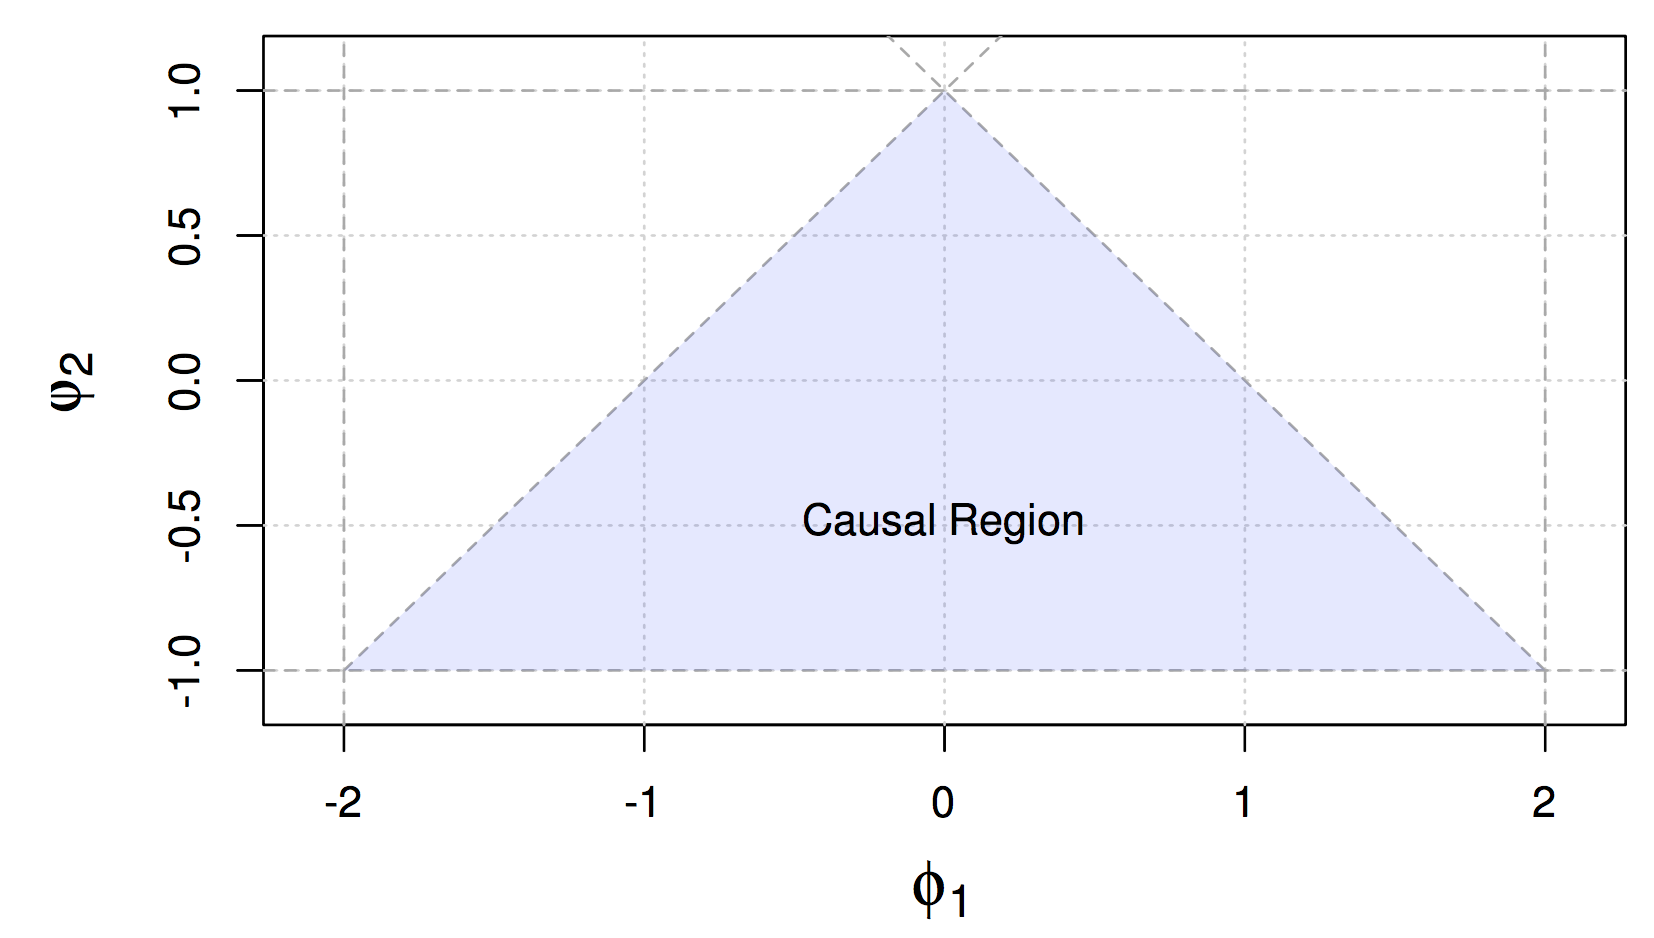
\includegraphics{images/causal_AR2} 

}

\caption{Causal Region for Parameters of an AR(2) Process}\label{fig:correxample2}
\end{figure}

\subsection{Estimation of AR(p) models}\label{estimation-of-arp-models}

Given the above defined properties of AR(p) models, we will now discuss
how these models can be estimated, more specifically how the \(p+1\)
parameters can be obtained from an observed time series. Indeed, a
reliable estimation of these models is necessary in order to intepret
and describe different natural phenomena and/or forecast possible future
values of the time series.

A first approach builds upon the earlier definition of AR(\(p\)) models
being a linear process. Recall that

\begin{equation}
    X_t = \sum_{j = 1}^{p} \phi_j X_{t-j}
\end{equation}

which delivers the following autocovariance function

\begin{equation}
    \gamma(h) = \text{cov}(X_{t+h}, X_t) = \text{cov}\left(\sum_{j = 1}^{p} \phi_j X_{t+h-j}, X_t\right) = \sum_{j = 1}^{p} \phi_j \gamma(h-j), \mbox{ } h \geq 1.
\end{equation}

Rearranging the above expressions we obtain the following general
equations

\begin{equation}
    \gamma(h) - \sum_{j = 1}^{p} \phi_j \gamma(h-j) = 0, \mbox{ } h \geq 1
\end{equation}

and, recalling that \(\gamma(h) = \gamma(-h)\),

\begin{equation}
    \gamma(0) - \sum_{j = 1}^{p} \phi_j \gamma(j) = \sigma_w^2.
\end{equation}

We can now define the Yule-Walker equations.

\textbf{Definition:} The Yule-Walker equations are given by

\begin{equation}
    \gamma(h) = \phi_1 \gamma(h-1) + ... + \phi_p \gamma(h-p), \mbox{ } h = 1,...,p
\end{equation}

and

\begin{equation}
    \sigma_w^2 = \gamma(0) - \phi_1 \gamma(1) - ... - \phi_p \gamma(p).
\end{equation}

which in matrix notation can be defined as follows

\begin{equation}
    \Gamma_p \mathbf{\phi} = \mathbf{\gamma}_p \,\, \text{and} \,\, \sigma_w^2 = \gamma(0) - \mathbf{\phi}'\mathbf{\gamma}_p
\end{equation}

where \(\Gamma_p\) is the \(p\times p\) matrix containing the
autocovariances \(\gamma(k-j)\), where \(j,k = 1, ...,p\), while
\(\mathbf{\phi} = (\phi_1,...,\phi_p)'\) and
\(\mathbf{\gamma}_p = (\gamma(1),...,\gamma(p))'\) are \(p\times 1\)
vectors.

Considering the Yule-Walker equations, it is possible to use a method of
moments approach and simply replace the theoretical quantities given in
the previous definition with their empirical (estimated) counterparts
that we saw in the previous chapter. This gives us the following
Yule-Walker estimators

\begin{equation}
    \hat{\mathbf{\phi}} = \hat{\Gamma}_p^{-1}\hat{\mathbf{\gamma}}_p \,\, \text{and} \,\, \hat{\sigma}_w^2 = \hat{\gamma}(0) - \hat{\mathbf{\gamma}}_p'\hat{\Gamma}_p^{-1}\hat{\mathbf{\gamma}}_p .
\end{equation}

These estimators have the following asymptotic properties.

\textbf{Consistency and Asymptotic Normality of Yule-Walker estimators:}
The Yule-Walker estimators for a causal AR(\(p\)) model have the
following asymptotic properties:

\begin{equation*}
\sqrt{T}(\hat{\mathbf{\phi}}- \mathbf{\phi}) \xrightarrow{\mathcal{D}} \mathcal{N}(\mathbf{0},\sigma_w^2\Gamma_p^{-1}) \,\, \text{and} \,\, \hat{\sigma}_w^2 \xrightarrow{\mathcal{P}} \sigma_w^2 .
\end{equation*}

Therefore the Yule-Walker estimators have an asymptotically normal
distribution and the estimator of the innovation variance is consistent.
Moreover, these estimators are also optimal for AR(\(p\)) models,
meaning that they are also efficient. However, there is also another
method which allows to achieve this efficiency (also for general ARMA
models that will be tackled further on) and this is the Maximum
Likelihood Estimation (MLE) method. Considering an AR(1) model as an
example, and assuming without loss of generality that its expectation is
zero, we have the following representation of the AR(1) model

\begin{equation*}
X_t = \phi X_{t-1} + W_t,
\end{equation*}

where \(|\phi|<1\) and
\(W_t \overset{iid}{\sim} \mathcal{N}(0,\sigma_w^2)\). Supposing we have
observations \((x_t)_{t=1,...,T}\) issued from this model, then the
likelihood function for this setting is given by

\begin{equation*}
L(\phi,\sigma_w^2) = f(\phi,\sigma_w^2|x_1,...,x_T)
\end{equation*}

which, for an AR(1) model, can be rewritten as follows

\begin{equation*}
L(\phi,\sigma_w^2) = f(x_1)f(x_2|x_1)\cdot \cdot \cdot f(x_T|x_{T-1}).
\end{equation*}

If we define \(\Omega_t^p\) as the information contained in the previous
\(p\) observations (before time \(t\)), the above expression can be
generalized for an AR(p) model as follows

\begin{equation*}
L(\phi,\sigma_w^2) = f(x_1,...,x_p)f(x_{p+1}|\Omega_{p+1}^p)\cdot \cdot \cdot f(x_T|\Omega_{T}^p)
\end{equation*}

where \(f(x_1,...,x_p)\) is the joint probability distribution of the
first \(p\) observations. Going back to the AR(1) setting, based on our
assumption on \((W_t)\) we know that
\(x_t|x_{t-1} \sim \mathcal{N}(\phi x_{t-1},\sigma_w^2)\) and therefore
we have that

\begin{equation*}
f(x_t|x_{t-1}) = f_w(x_t - \phi x_{t-1})
\end{equation*}

where \(f_w(\cdot)\) is the distribution of \(W_t\). This rearranges the
likelihood function as follows

\begin{equation*}
L(\phi,\sigma_w^2) = f(x_1)\prod_{t=2}^T f_w(x_t - \phi x_{t-1}),
\end{equation*}

where \(f(x_1)\) can be found through the causal representation

\begin{equation*}
x_1 = \sum_{j=0}^{\infty} \phi^j w_{1-j},
\end{equation*}

which implies that \(x_1\) follows a normal distribution with zero
expectation and a variance given by \(\frac{\sigma_w^2}{(1-\phi^2)}\).
Based on this, the likelihood function of an AR(1) finally becomes

\begin{equation*}
L(\phi,\sigma_w^2) = (2\pi \sigma_w^2)^{-\frac{T}{2}} (1 - \phi^2)^{\frac{1}{2}} \exp \left(-\frac{S(\phi)}{2 \sigma_w^2}\right),
\end{equation*}

with
\(S(\phi) = (1-\phi^2) x_1^2 + \sum_{t=2}^T (x_t -\phi x_{t-1})^2\).
Once the derivative of the logarithm of the likelihood is taken, the
minimization of the negative of this function is usually done
numerically. However, if we condition on the initial values, the AR(p)
models are linear and, for example, we can then define the conditional
likelihood of an AR(1) as

\begin{equation*}
L(\phi,\sigma_w^2|x_1) = (2\pi \sigma_w^2)^{-\frac{T-1}{2}} \exp \left(-\frac{S_c(\phi)}{2 \sigma_w^2}\right),
\end{equation*}

where

\begin{equation*}
S_c(\phi) = \sum_{t=2}^T (x_t -\phi x_{t-1})^2 .
\end{equation*}

The latter is called the conditional sum of squares and \(\phi\) can be
estimated as a straightforward linear regression problem. Once an
estimate \(\hat{\phi}\) is obtained, this can be used to obtain the
conditional maximum likelihood estimate of \(\sigma_w^2\)

\begin{equation*}
\hat{\sigma}_w^2 = \frac{S_c(\hat{\phi})}{(T-1)} .
\end{equation*}

The estimation methods presented so far are standard for these kind of
models. Nevertheless, if the data suffers from some form of
contamination, these methods can become highly biased. For this reason,
some robust estimators are available to limit this problematic if there
are indeed outliers in the observed time series. One of these methods
relies on the estimator proposed in Kunsch (1984) who underlines that
the MLE score function of an AR(p) is given by

\begin{equation*}
 \kappa(\mathbf{\theta}|x_j,...x_{j+p}) = \frac{\partial}{\partial \mathbf{\theta}} (x_{j+p} - \sum_{k=1}^p \phi_k x_{j+p-k})^2,
\end{equation*}

where \(\theta\) is the parameter vector containing, in the case of an
AR(1) model, the two parameters \(\phi\) and \(\sigma_w^2\) (i.e.
\(\theta = [\phi \,\, \sigma_w^2]\)). This delivers the estimating
equation

\begin{equation*}
\sum_{j=1}^{n-p} \kappa (\hat{\mathbf{\theta}}|x_j,...x_{j+p}) = 0 .
\end{equation*}

The score function \(\kappa(\cdot)\) is clearly not bounded, in the
sense that if we arbitrarily move a value of \((x_t)\) to infinity then
the score function also goes to infinity thereby delivering a biased
estimation procedure. To avoid that outlying observations bias the
estimation excessively, a bounded score function can be used to deliver
an M-estimator given by

\begin{equation*}
\sum_{j=1}^{n-p} \psi (\hat{\mathbf{\theta}}|x_j,...x_{j+p}) = 0,
\end{equation*}

where \(\psi(\cdot)\) is a function of bounded variation. When
conditioning on the first \(p\) observations, this problem can be
brought back to a linear regression problem which can be applied in a
robust manner using the robust regression tools available in \texttt{R}
such as \texttt{rlm} or \texttt{lmrob}. However, another available tool
in \texttt{R} which does not require a strict specification of the
distribution function (also for general ARMA models) is the
\texttt{method\ =\ "rgmwm"} option within the \texttt{estimate()}
function (in the \texttt{simts} package). This function makes use of a
quantity called the wavelet variance (denoted as \(\boldsymbol{\nu}\))
which is estimated robustly and then used to retrieve the parameters
\(\theta\) of the time series model. The robust estimate is obtained by
solving the following minimization problem

\begin{equation*}
\hat{\boldsymbol{\theta}} = \underset{\boldsymbol{\theta} \in \boldsymbol{\Theta}}{\text{argmin}} (\hat{\boldsymbol{\nu}} - \boldsymbol{\nu}(\boldsymbol{\theta}))^T\boldsymbol{\Omega}(\hat{\boldsymbol{\nu}} - \boldsymbol{\nu}({\boldsymbol{\theta}})),
\end{equation*}

where \(\hat{\boldsymbol{\nu}}\) is the robustly estimated wavelet
variance, \(\boldsymbol{\nu}({\boldsymbol{\theta}})\) is the theoretical
wavelet variance (implied by the model we want to estimate) and
\(\boldsymbol{\Omega}\) is a positive definite weighting matrix. Below
we show some simulation studies where we present the results of the
above estimation procedures in absence and in presence of contamination
in the data. As a reminder, so far we have mainly discussed three
estimators for the parameters of AR(\(p\)) models (i.e. Yule-Walker,
maximum likelihod, and RGMWM estimators).

Using the \texttt{simts} package, the first three estimators can be
computed as follows:

\begin{Shaded}
\begin{Highlighting}[]
\NormalTok{mod =}\StringTok{ }\KeywordTok{estimate}\NormalTok{(}\KeywordTok{AR}\NormalTok{(p), Xt, }\DataTypeTok{method =}\NormalTok{ select_method, }\DataTypeTok{demean =} \OtherTok{TRUE}\NormalTok{)}
\end{Highlighting}
\end{Shaded}

In the above sample code \texttt{Xt} denotes the time series (a vector
of length \(T\)), \texttt{p} is the order of the AR(\(p\)) and
\texttt{demean\ =\ TRUE} indicates that the mean of the process should
be estimated (if this is not the case, then use
\texttt{demean\ =\ FALSE}). The \texttt{select\_method} input can be
(among others) \texttt{"mle"} for the maximum likelihood and
\texttt{"yule-walker"} for the Yule-Walker estimator or \texttt{"rgmwm"}
for the RGMWM. For example, if you would like to estimate a zero mean
AR(3) with the MLE you can use the code:

\begin{Shaded}
\begin{Highlighting}[]
\NormalTok{mod =}\StringTok{ }\KeywordTok{estimate}\NormalTok{(}\KeywordTok{AR}\NormalTok{(}\DecValTok{3}\NormalTok{), Xt, }\DataTypeTok{method =} \StringTok{"mle"}\NormalTok{, }\DataTypeTok{demean =} \OtherTok{FALSE}\NormalTok{)}
\end{Highlighting}
\end{Shaded}

On the other hand, if one wishes to estimate the parameters of this
model through the RGMWM one can use the following syntax:

\begin{Shaded}
\begin{Highlighting}[]
\NormalTok{mod =}\StringTok{ }\KeywordTok{estimate}\NormalTok{(}\KeywordTok{AR}\NormalTok{(}\DecValTok{3}\NormalTok{), Xt, }\DataTypeTok{method =} \StringTok{"rgmwm"}\NormalTok{, }\DataTypeTok{demean =} \OtherTok{FALSE}\NormalTok{)}
\end{Highlighting}
\end{Shaded}

Removing the mean is not strictly necessary for the \texttt{rgmwm} (or
\texttt{gmwm}) function since it won't estimate it and can consistently
estimate the parameters of the time series model anyway. We now have the
necessary \texttt{R} functions to deliver the above mentioned estimators
and we can now proceed to the simulation study. In particular, we
simulate three different processes \(X_t, Y_t, Z_t\) by using the first
as an uncontaminated process defined as
\[X_t = 0.5 X_{t-1} - 0.25 X_{t-2} + W_t,\] with
\(W_t \overset{iid}{\sim} N(0, 1)\). This first process \((X_t)\) is
uncontaminated while the other two processes are contaminated versions
of the first that can often be observed in practice. The first type of
contamination can be seen in \((Y_t)\) and is delivered by replacing a
portion of the original process with a process defined as
\[U_t = 0.90 U_{t-1} - 0.40 U_{t-2} + V_t,\] where
\(V_t \overset{iid}{\sim} N(0, 9)\). The second form of contamination
can be seen in \((Z_t)\) and consists in the so-called point-wise
contamination where randomly selected points from \(X_t\) are replaced
with \(N_t \overset{iid}{\sim} N(0, 9)\).

The code below performs the simulation study where it can be seen how
the contaminated processes \((Y_t)\) and \((Z_t)\) are generated. Once
this is done, for each simultation the code estimates the parameters of
the AR(2) model using the three different estimation methods.

\begin{Shaded}
\begin{Highlighting}[]
\CommentTok{# Load simts}
\KeywordTok{library}\NormalTok{(simts)}

\CommentTok{# Number of bootstrap iterations}
\NormalTok{B =}\StringTok{ }\DecValTok{250}

\CommentTok{# Sample size}
\NormalTok{n =}\StringTok{ }\DecValTok{500}

 \CommentTok{# Proportion of contamination}
\NormalTok{eps =}\StringTok{ }\FloatTok{0.05}       

\CommentTok{# Number of contaminated observations}
\NormalTok{cont =}\StringTok{ }\KeywordTok{round}\NormalTok{(eps}\OperatorTok{*}\NormalTok{n)   }

\CommentTok{# Simulation storage}
\NormalTok{res.Xt.MLE =}\StringTok{ }\NormalTok{res.Xt.YW =}\StringTok{ }\NormalTok{res.Xt.RGMWM =}\StringTok{ }\KeywordTok{matrix}\NormalTok{(}\OtherTok{NA}\NormalTok{, B, }\DecValTok{3}\NormalTok{)}
\NormalTok{res.Yt.MLE =}\StringTok{ }\NormalTok{res.Yt.YW =}\StringTok{ }\NormalTok{res.Yt.RGMWM =}\StringTok{ }\KeywordTok{matrix}\NormalTok{(}\OtherTok{NA}\NormalTok{, B, }\DecValTok{3}\NormalTok{)}
\NormalTok{res.Zt.MLE =}\StringTok{ }\NormalTok{res.Zt.YW =}\StringTok{ }\NormalTok{res.Zt.RGMWM =}\StringTok{ }\KeywordTok{matrix}\NormalTok{(}\OtherTok{NA}\NormalTok{, B, }\DecValTok{3}\NormalTok{)}
  
\CommentTok{# Begin bootstrap}
\ControlFlowTok{for}\NormalTok{ (i }\ControlFlowTok{in} \KeywordTok{seq_len}\NormalTok{(B))\{}
  \CommentTok{# Set seed for reproducibility}
  \KeywordTok{set.seed}\NormalTok{(}\DecValTok{1982} \OperatorTok{+}\StringTok{ }\NormalTok{i)}
  
  \CommentTok{# Generate processes}
\NormalTok{  Xt =}\StringTok{ }\KeywordTok{gen_gts}\NormalTok{(n, }\KeywordTok{AR}\NormalTok{(}\DataTypeTok{phi =} \KeywordTok{c}\NormalTok{(}\FloatTok{0.5}\NormalTok{, }\FloatTok{0.25}\NormalTok{), }\DataTypeTok{sigma2 =} \DecValTok{1}\NormalTok{))}
\NormalTok{  Yt =}\StringTok{ }\NormalTok{Zt =}\StringTok{ }\NormalTok{Xt}
  
  \CommentTok{# Generate Ut contamination process that replaces a portion of original signal}
\NormalTok{  index_start =}\StringTok{ }\KeywordTok{sample}\NormalTok{(}\DecValTok{1}\OperatorTok{:}\NormalTok{(n}\OperatorTok{-}\NormalTok{cont}\OperatorTok{-}\DecValTok{1}\NormalTok{), }\DecValTok{1}\NormalTok{)}
\NormalTok{  index_end =}\StringTok{ }\NormalTok{index_start }\OperatorTok{+}\StringTok{ }\NormalTok{cont }\OperatorTok{-}\StringTok{ }\DecValTok{1}
\NormalTok{  Yt[index_start}\OperatorTok{:}\NormalTok{index_end] =}\StringTok{ }\KeywordTok{gen_gts}\NormalTok{(cont, }\KeywordTok{AR}\NormalTok{(}\DataTypeTok{phi =} \KeywordTok{c}\NormalTok{(}\FloatTok{0.9}\NormalTok{,}\OperatorTok{-}\FloatTok{0.4}\NormalTok{), }\DataTypeTok{sigma2 =} \DecValTok{9}\NormalTok{))}
  
  \CommentTok{# Generate Nt contamination that inject noise at random}
\NormalTok{  Zt[}\KeywordTok{sample}\NormalTok{(n, cont, }\DataTypeTok{replace =} \OtherTok{FALSE}\NormalTok{)] =}\StringTok{ }\KeywordTok{gen_gts}\NormalTok{(cont, }\KeywordTok{WN}\NormalTok{(}\DataTypeTok{sigma2 =} \DecValTok{9}\NormalTok{))}
  
  \CommentTok{# Fit Yule-Walker estimators on the three time series}
\NormalTok{  mod.Xt.YW =}\StringTok{ }\KeywordTok{estimate}\NormalTok{(}\KeywordTok{AR}\NormalTok{(}\DecValTok{2}\NormalTok{), Xt, }\DataTypeTok{method =} \StringTok{"yule-walker"}\NormalTok{, }
                 \DataTypeTok{demean =} \OtherTok{FALSE}\NormalTok{)}
\NormalTok{  mod.Yt.YW =}\StringTok{ }\KeywordTok{estimate}\NormalTok{(}\KeywordTok{AR}\NormalTok{(}\DecValTok{2}\NormalTok{), Yt, }\DataTypeTok{method =} \StringTok{"yule-walker"}\NormalTok{, }
                 \DataTypeTok{demean =} \OtherTok{FALSE}\NormalTok{)}
\NormalTok{  mod.Zt.YW =}\StringTok{ }\KeywordTok{estimate}\NormalTok{(}\KeywordTok{AR}\NormalTok{(}\DecValTok{2}\NormalTok{), Zt, }\DataTypeTok{method =} \StringTok{"yule-walker"}\NormalTok{, }
                 \DataTypeTok{demean =} \OtherTok{FALSE}\NormalTok{)}
  
  \CommentTok{# Store results}
\NormalTok{  res.Xt.YW[i, ] =}\StringTok{ }\KeywordTok{c}\NormalTok{(mod.Xt.YW}\OperatorTok{$}\NormalTok{mod}\OperatorTok{$}\NormalTok{coef, mod.Xt.YW}\OperatorTok{$}\NormalTok{mod}\OperatorTok{$}\NormalTok{sigma2)}
\NormalTok{  res.Yt.YW[i, ] =}\StringTok{ }\KeywordTok{c}\NormalTok{(mod.Yt.YW}\OperatorTok{$}\NormalTok{mod}\OperatorTok{$}\NormalTok{coef, mod.Yt.YW}\OperatorTok{$}\NormalTok{mod}\OperatorTok{$}\NormalTok{sigma2)}
\NormalTok{  res.Zt.YW[i, ] =}\StringTok{ }\KeywordTok{c}\NormalTok{(mod.Zt.YW}\OperatorTok{$}\NormalTok{mod}\OperatorTok{$}\NormalTok{coef, mod.Zt.YW}\OperatorTok{$}\NormalTok{mod}\OperatorTok{$}\NormalTok{sigma2)}
  

  \CommentTok{# Fit MLE on the three time series}
\NormalTok{  mod.Xt.MLE =}\StringTok{ }\KeywordTok{estimate}\NormalTok{(}\KeywordTok{AR}\NormalTok{(}\DecValTok{2}\NormalTok{), Xt, }\DataTypeTok{method =} \StringTok{"mle"}\NormalTok{, }
                 \DataTypeTok{demean =} \OtherTok{FALSE}\NormalTok{)}
\NormalTok{  mod.Yt.MLE =}\StringTok{ }\KeywordTok{estimate}\NormalTok{(}\KeywordTok{AR}\NormalTok{(}\DecValTok{2}\NormalTok{), Yt, }\DataTypeTok{method =} \StringTok{"mle"}\NormalTok{, }
                 \DataTypeTok{demean =} \OtherTok{FALSE}\NormalTok{)}
\NormalTok{  mod.Zt.MLE =}\StringTok{ }\KeywordTok{estimate}\NormalTok{(}\KeywordTok{AR}\NormalTok{(}\DecValTok{2}\NormalTok{), Zt, }\DataTypeTok{method =} \StringTok{"mle"}\NormalTok{, }
                 \DataTypeTok{demean =} \OtherTok{FALSE}\NormalTok{)}
  
  \CommentTok{# Store results}
\NormalTok{  res.Xt.MLE[i, ] =}\StringTok{ }\KeywordTok{c}\NormalTok{(mod.Xt.MLE}\OperatorTok{$}\NormalTok{mod}\OperatorTok{$}\NormalTok{coef, mod.Xt.MLE}\OperatorTok{$}\NormalTok{mod}\OperatorTok{$}\NormalTok{sigma2)}
\NormalTok{  res.Yt.MLE[i, ] =}\StringTok{ }\KeywordTok{c}\NormalTok{(mod.Yt.MLE}\OperatorTok{$}\NormalTok{mod}\OperatorTok{$}\NormalTok{coef, mod.Yt.MLE}\OperatorTok{$}\NormalTok{mod}\OperatorTok{$}\NormalTok{sigma2)}
\NormalTok{  res.Zt.MLE[i, ] =}\StringTok{ }\KeywordTok{c}\NormalTok{(mod.Zt.MLE}\OperatorTok{$}\NormalTok{mod}\OperatorTok{$}\NormalTok{coef, mod.Zt.MLE}\OperatorTok{$}\NormalTok{mod}\OperatorTok{$}\NormalTok{sigma2)}
  
  \CommentTok{# Fit RGMWM on the three time series}
\NormalTok{  res.Xt.RGMWM[i, ] =}\StringTok{ }\KeywordTok{estimate}\NormalTok{(}\KeywordTok{AR}\NormalTok{(}\DecValTok{2}\NormalTok{), Xt, }\DataTypeTok{method =} \StringTok{"rgmwm"}\NormalTok{, }
                 \DataTypeTok{demean =} \OtherTok{FALSE}\NormalTok{)}\OperatorTok{$}\NormalTok{mod}\OperatorTok{$}\NormalTok{estimate}
\NormalTok{  res.Yt.RGMWM[i, ] =}\StringTok{ }\KeywordTok{estimate}\NormalTok{(}\KeywordTok{AR}\NormalTok{(}\DecValTok{2}\NormalTok{), Yt, }\DataTypeTok{method =} \StringTok{"rgmwm"}\NormalTok{, }
                 \DataTypeTok{demean =} \OtherTok{FALSE}\NormalTok{)}\OperatorTok{$}\NormalTok{mod}\OperatorTok{$}\NormalTok{estimate}
\NormalTok{  res.Zt.RGMWM[i, ] =}\StringTok{ }\KeywordTok{estimate}\NormalTok{(}\KeywordTok{AR}\NormalTok{(}\DecValTok{2}\NormalTok{), Zt, }\DataTypeTok{method =} \StringTok{"rgmwm"}\NormalTok{, }
                 \DataTypeTok{demean =} \OtherTok{FALSE}\NormalTok{)}\OperatorTok{$}\NormalTok{mod}\OperatorTok{$}\NormalTok{estimate}
\NormalTok{\}}
\end{Highlighting}
\end{Shaded}

Having performed the estimation, we should now have 250 estimates for
each AR(2) parameter and each estimation method. The code below takes
the results of the simulation and shows them in the shape of boxplots
along with the true values of the parameters. The estimation methods
that are denoted as follows:

\begin{itemize}
\tightlist
\item
  \textbf{YW}: Yule-Walker estimator
\item
  \textbf{MLE}: Maximum Likelihood Estimator
\item
  \textbf{RGMWM}: the robust version of the GMWM estimator
\end{itemize}

\begin{figure}

{\centering 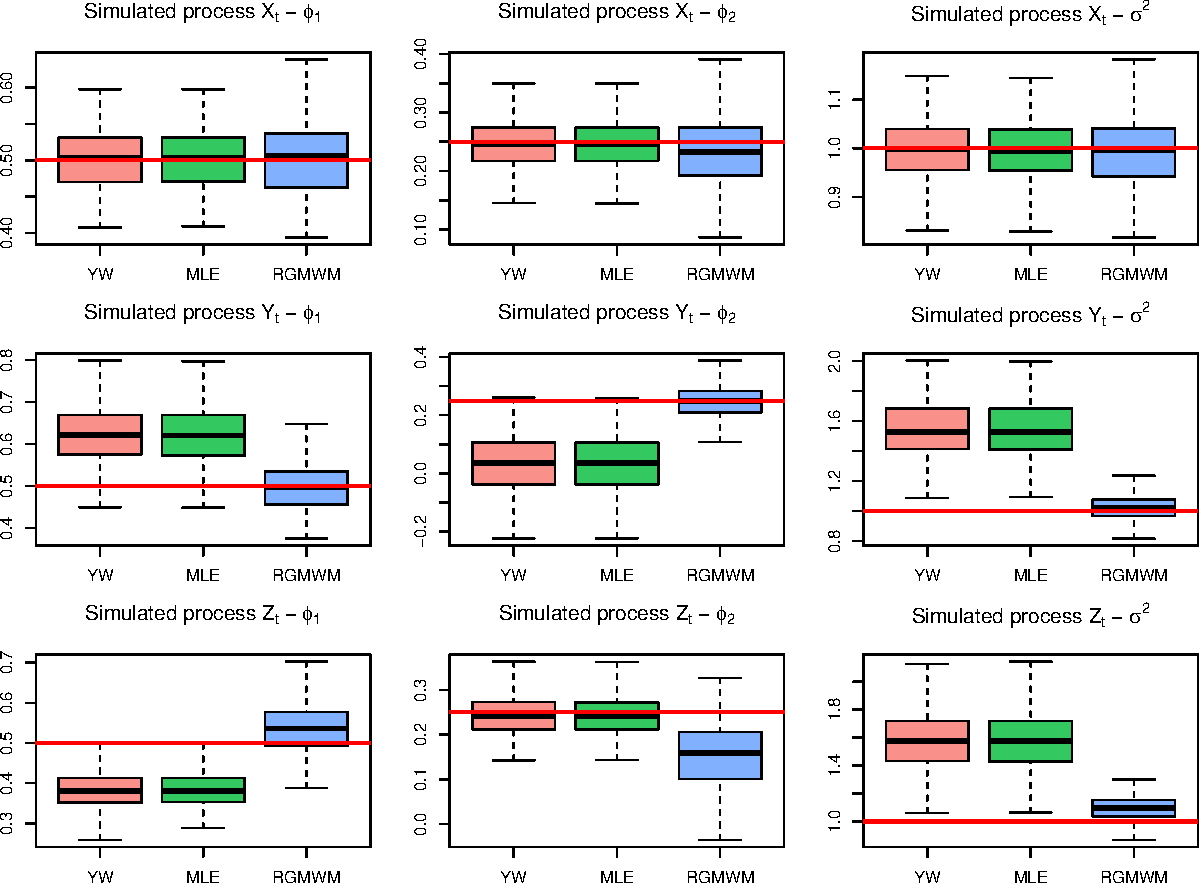
\includegraphics{ts_files/figure-latex/unnamed-chunk-30-1} 

}

\caption{Boxplots of the empirical distribution functions of the Yule-Walker (YW), MLE and GMWM estimators for the parameters of the AR(2) model when using the Xt process (first row of boxplots), Yt process (second row of boxplots) and Zt (third row of boxplots).}\label{fig:unnamed-chunk-30}
\end{figure}

It can be seen how all methods appear to properly estimate the true
parameter values on average when they are applied to the simulated time
series from the uncontaminated process \((X_t)\). However, the MLE
appears to be slightly more efficient (less variable) compared to the
other methods and, in addition, the robust method (RGMWM) appears to be
less efficient than the other two estimators. The latter is a known
result since robust estimators usually pay a price in terms of
efficiency (as an insurance against bias).

On the other hand, when checking the performance of the same methods
when applied to the two contaminated processes \((Y_t)\) and \((Z_t)\)
it can be seen that the standard estimators appear to be (highly) biased
for most of the estimated parameters (with one exception) while the
robust estimator remains close (on average) to the true parameter values
that we are aiming to estimate. Therefore, when there's a suspicion that
there could be some (small) contamination in the observed time series,
it may be more appropriate to use a robust estimator.

To conclude this section on estimation, we now compare the above studied
estimators in different applied settings where we can highlight how to
assess which estimator is more appropriate according to the type of
setting. For this purpose, let us start with an example we have already
checked in the previous chapter when discussing standard and robust
estimators of the ACF, more specifically the data on monthly
precipitations. As mentioned before when discussing this example, the
importance of modelling precipitation data lies in the fact that its
usually used to successively model the entire water cycle. Common models
for this purpose are either the white noise (WN) model or the AR(1)
model. Let us compare the standard and robust ACF again to understand
which of these two models seems more appropriate for the data at hand.

\begin{Shaded}
\begin{Highlighting}[]
\KeywordTok{compare_acf}\NormalTok{(hydro)}
\end{Highlighting}
\end{Shaded}

\begin{figure}

{\centering 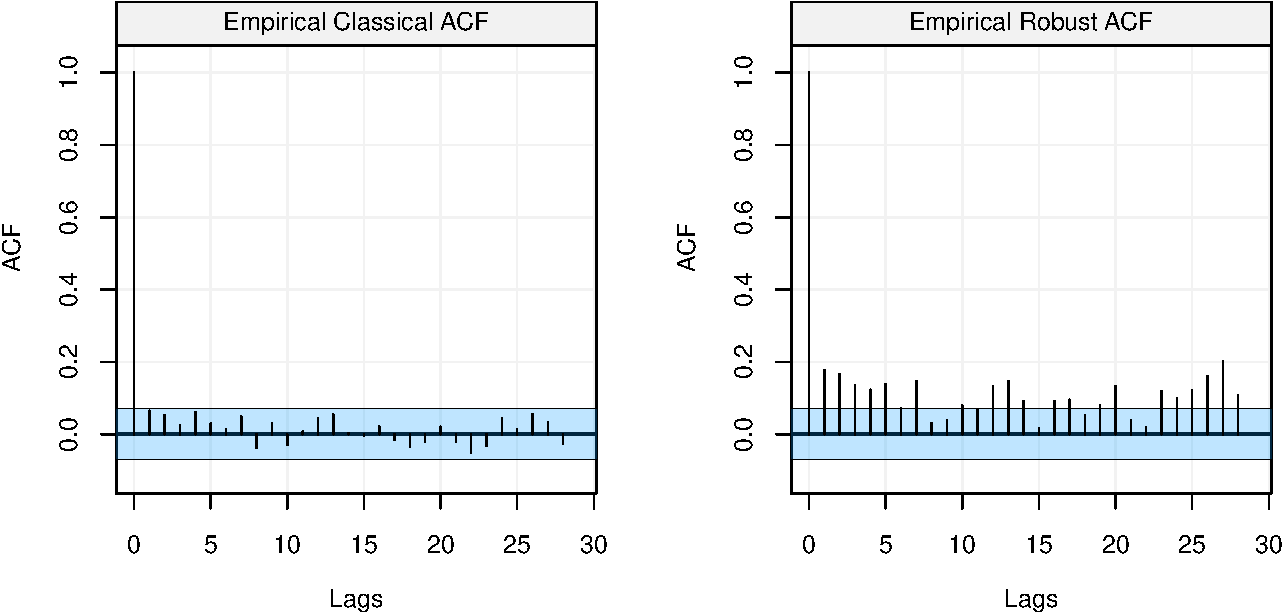
\includegraphics{ts_files/figure-latex/unnamed-chunk-31-1} 

}

\caption{Standard (left) and robust (left) estimates of the ACF function on the monthly precipitation data (hydro)}\label{fig:unnamed-chunk-31}
\end{figure}

As we had underlined in the previous chapter, the standard ACF estimates
would suggest that there appears to be no correlation among lags and
consequently, the WN model would be the most appropriate. However, the
robust ACF estimates depict an entirely different picture where it can
be seen that there appears to be a significant autocorrelation over
different lags which exponentially decay. Although there appears to be
some seasonality in the plot, we will assume that the correct model for
this data is an AR(1) since that's what hydrology theory suggests. Let
us therefore estimate the parameters of this model by using a standard
estimator (MLE) and a robust estimator (RGMWM). The estimates for the
MLE are the following:

\begin{Shaded}
\begin{Highlighting}[]
\NormalTok{mle_hydro =}\StringTok{ }\KeywordTok{estimate}\NormalTok{(}\KeywordTok{AR}\NormalTok{(}\DecValTok{1}\NormalTok{), }\KeywordTok{as.vector}\NormalTok{(hydro),  }\DataTypeTok{method =} \StringTok{"mle"}\NormalTok{, }\DataTypeTok{demean =} \OtherTok{TRUE}\NormalTok{)}

\CommentTok{# MLE Estimates}
\KeywordTok{c}\NormalTok{(mle_hydro}\OperatorTok{$}\NormalTok{mod}\OperatorTok{$}\NormalTok{coef[}\DecValTok{1}\NormalTok{], mle_hydro}\OperatorTok{$}\NormalTok{mod}\OperatorTok{$}\NormalTok{sigma2)}
\end{Highlighting}
\end{Shaded}

\begin{verbatim}
##        ar1            
## 0.06497727 0.22205713
\end{verbatim}

From these estimates it would appear that the autocorrelation between
lagged variables (i.e.~lags of order 1) is extremely low and that (as
suggested by the standard ACF plot) a WN model may be more appropriate.
Considering the robust ACF however, it is possible that the MLE
estimates may not be reliable in this setting. Hence, let us use the
RGMWM to estimate the same parameters.

\begin{Shaded}
\begin{Highlighting}[]
\NormalTok{rgmwm_hydro =}\StringTok{ }\KeywordTok{estimate}\NormalTok{(}\KeywordTok{AR}\NormalTok{(}\DecValTok{1}\NormalTok{), hydro, }\DataTypeTok{method =} \StringTok{"rgmwm"}\NormalTok{)}\OperatorTok{$}\NormalTok{mod}\OperatorTok{$}\NormalTok{estimate}

\CommentTok{# RGMWM Estimates}
\KeywordTok{t}\NormalTok{(rgmwm_hydro)}
\end{Highlighting}
\end{Shaded}

\begin{verbatim}
##                  AR    SIGMA2
## Estimates 0.4048702 0.1065875
\end{verbatim}

In this case, we see how the autocorrelation between lagged values is
much higher (0.4 compared to 0.06) indicating that there is a stronger
dependence in the data than what is suggested by standard estimators.
Moreover, the innovation variance is smaller compared to that of the
MLE. This is also a known phenomenon when there's contamination in the
data since it leads to less dependence and more variability being
detected by non-robust estimators. This estimate of the variance also
has a considerable impact on forecast precision (as we'll see in the
next section).

A final applied example that highlights the (potential) difference
between estimators according to the type of setting is given by the
``Recruitment'' data set (in the \texttt{astsa} library). This data
refers to the presence of new fish in the population of the Pacific
Ocean and is often linked to the currents and temperatures passing
through the ocean. As for the previous data set, let us take a look at
the data itself and then analyse the standard and robust estimations of
the ACF.

\begin{Shaded}
\begin{Highlighting}[]
\CommentTok{# Format data}
\NormalTok{fish =}\StringTok{ }\KeywordTok{gts}\NormalTok{(rec, }\DataTypeTok{start =} \DecValTok{1950}\NormalTok{, }\DataTypeTok{freq =} \DecValTok{12}\NormalTok{, }\DataTypeTok{unit_time =} \StringTok{'month'}\NormalTok{, }\DataTypeTok{name_ts =} \StringTok{'Recruitment'}\NormalTok{)}

\CommentTok{# Plot data}
\KeywordTok{plot}\NormalTok{(fish)}
\end{Highlighting}
\end{Shaded}

\begin{figure}

{\centering 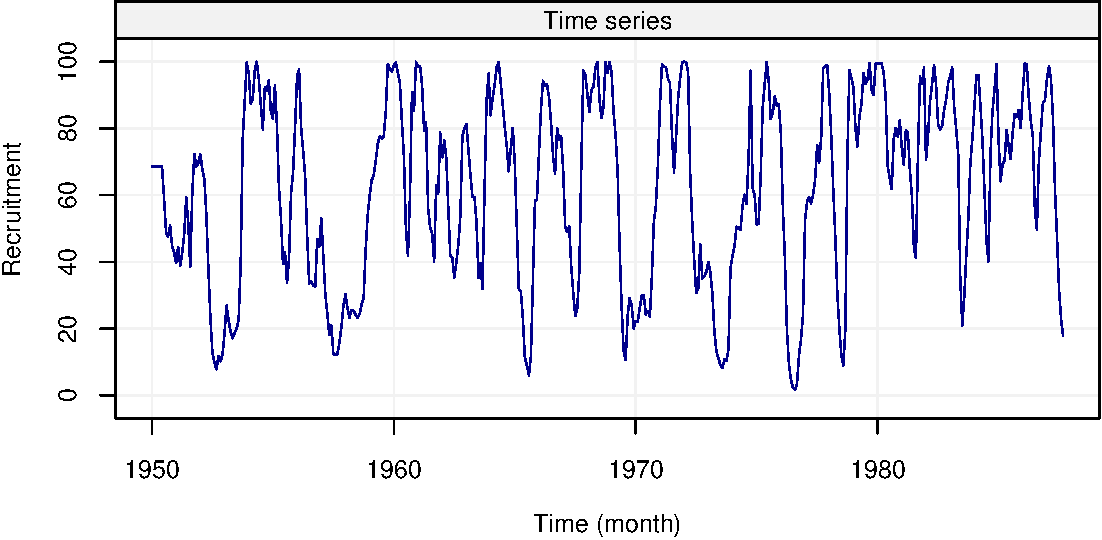
\includegraphics{ts_files/figure-latex/unnamed-chunk-35-1} 

}

\caption{Plot of the time series on fish recruitment monthly data in the Pacific Ocean from 1950 to 1987}\label{fig:unnamed-chunk-35}
\end{figure}

\begin{Shaded}
\begin{Highlighting}[]
\KeywordTok{compare_acf}\NormalTok{(fish)}
\end{Highlighting}
\end{Shaded}

\begin{figure}

{\centering 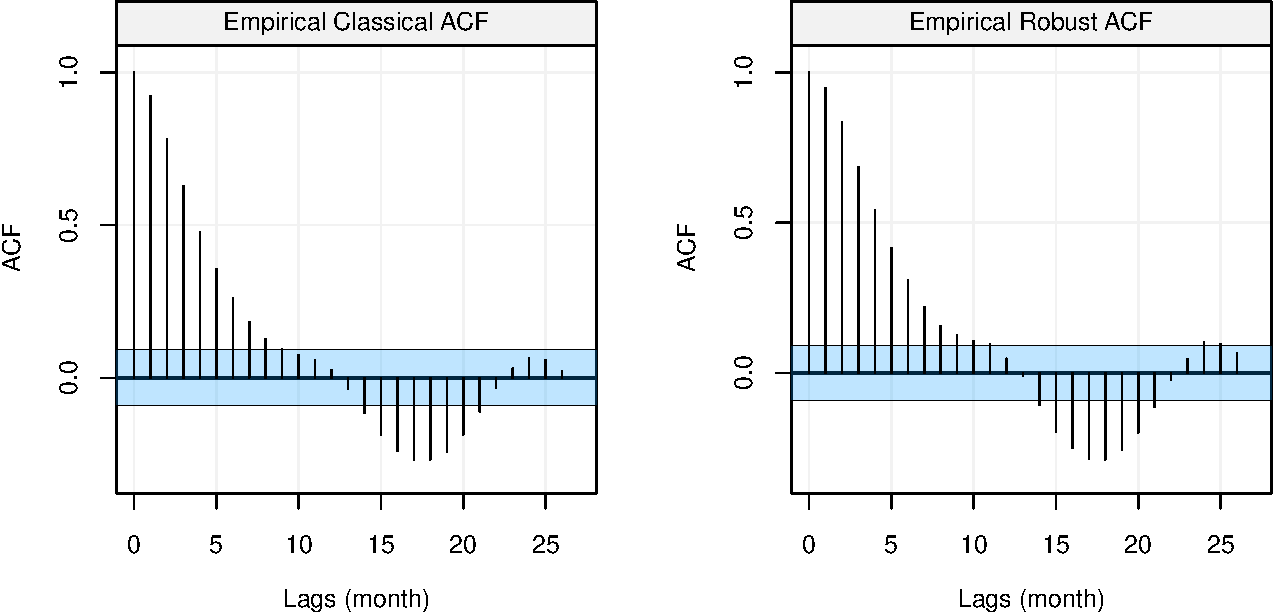
\includegraphics{ts_files/figure-latex/unnamed-chunk-36-1} 

}

\caption{Standard (left) and robust (left) estimates of the ACF function on the monthly fish recruitment data (rec)}\label{fig:unnamed-chunk-36}
\end{figure}

We can see that there appears to be a considerable dependence between
the lagged variables which decays (in a similar way to the ACF of an
AR(\(p\))). Also in this case we see a seasonality in the data but we
won't consider this for the purpose of this example. Given that there
doesn't appear to be any significant contamination in the data, let us
consider the Yule-Walker and MLE estimators. The MLE highly depends on
the assumed parametric distribution of the time series (i.e.~usually
Gaussian) and, if this is not respected, the resulting estimations could
be unreliable. Hence, a first difference of the time series can often
give an idea of the marginal distribution of the time series.

\begin{Shaded}
\begin{Highlighting}[]
\CommentTok{# Take first differencing of the recruitment data}
\NormalTok{diff_fish =}\StringTok{ }\KeywordTok{gts}\NormalTok{(}\KeywordTok{diff}\NormalTok{(rec), }\DataTypeTok{start =} \DecValTok{1950}\NormalTok{, }\DataTypeTok{freq =} \DecValTok{12}\NormalTok{, }\DataTypeTok{unit_time =} \StringTok{'month'}\NormalTok{, }\DataTypeTok{name_ts =} \StringTok{'Recruitment'}\NormalTok{)}

\CommentTok{# Plot first differencing of the recruitment data}
\KeywordTok{plot}\NormalTok{(diff_fish)}
\end{Highlighting}
\end{Shaded}

\begin{figure}

{\centering 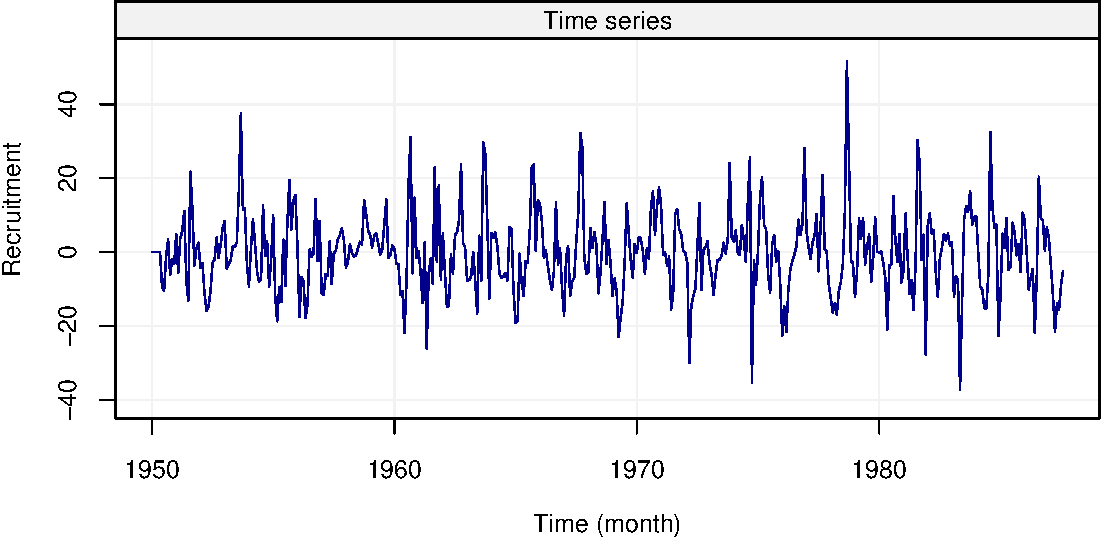
\includegraphics{ts_files/figure-latex/unnamed-chunk-38-1} 

}

\caption{Plot of the first difference of the time series on fish recruitment monthly data in the Pacific Ocean from 1950 to 1987}\label{fig:unnamed-chunk-38}
\end{figure}

From the plot we can see that observations appear to be collected around
a constant value and fewer appear to be further from this value (as
would be the case for a normal distribution). However, various of these
``more extreme'' observations appear to be quite frequent suggesting
that the underlying distribution may have a heavier tail compared to the
normal distribution. Let us compare the standard and robust ACF
estimates of this new time series.

\begin{Shaded}
\begin{Highlighting}[]
\KeywordTok{compare_acf}\NormalTok{(diff_fish)}
\end{Highlighting}
\end{Shaded}

\begin{figure}

{\centering 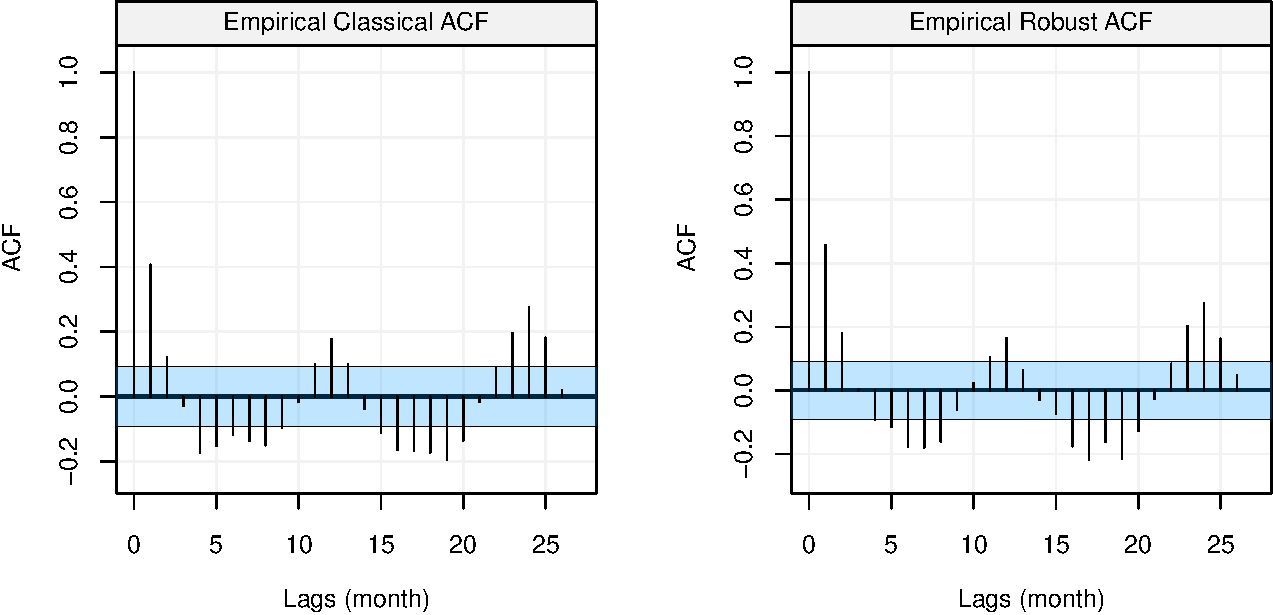
\includegraphics{ts_files/figure-latex/unnamed-chunk-39-1} 

}

\caption{Standard (left) and robust (left) estimates of the ACF function on the first difference of the monthly fish recruitment data (rec)}\label{fig:unnamed-chunk-39}
\end{figure}

In this case we see that the patterns appear to be the same but the
values between the standard and robust estimates are slightly (to
moderately) different over different lags. This would suggest that there
could be some contamination in the data or, in any case, that the normal
assumption may not hold exactly. With this in mind, let us estimate an
AR(2) model for this data using the Yule-Walker and MLE.

\begin{Shaded}
\begin{Highlighting}[]
\CommentTok{# MLE of Recruitment data}
\NormalTok{yw_fish =}\StringTok{ }\KeywordTok{estimate}\NormalTok{(}\KeywordTok{AR}\NormalTok{(}\DecValTok{2}\NormalTok{), rec, }\DataTypeTok{method =} \StringTok{"yule-walker"}\NormalTok{, }\DataTypeTok{demean =} \OtherTok{TRUE}\NormalTok{)}

\CommentTok{# MLE of Recruitment data}
\NormalTok{mle_fish =}\StringTok{ }\KeywordTok{estimate}\NormalTok{(}\KeywordTok{AR}\NormalTok{(}\DecValTok{2}\NormalTok{), rec, }\DataTypeTok{method =} \StringTok{"mle"}\NormalTok{, }\DataTypeTok{demean =} \OtherTok{TRUE}\NormalTok{)}

\CommentTok{# Compare estimates}
\CommentTok{# Yule-Walker Estimation}
\KeywordTok{c}\NormalTok{(yw_fish}\OperatorTok{$}\NormalTok{mod}\OperatorTok{$}\NormalTok{coef[}\DecValTok{1}\NormalTok{], yw_fish}\OperatorTok{$}\NormalTok{mod}\OperatorTok{$}\NormalTok{sigma2)}
\end{Highlighting}
\end{Shaded}

\begin{verbatim}
##       ar1           
##  1.354069 89.717052
\end{verbatim}

\begin{Shaded}
\begin{Highlighting}[]
\CommentTok{# MLE Estimation}
\KeywordTok{c}\NormalTok{(mle_fish}\OperatorTok{$}\NormalTok{mod}\OperatorTok{$}\NormalTok{coef[}\DecValTok{1}\NormalTok{], mle_fish}\OperatorTok{$}\NormalTok{mod}\OperatorTok{$}\NormalTok{sigma2)}
\end{Highlighting}
\end{Shaded}

\begin{verbatim}
##       ar1           
##  1.351218 89.334361
\end{verbatim}

It can be seen that, in this setting, the two estimators deliver very
similar results (at least in terms of the \(\phi_1\) and \(\phi_2\)
coefficients). Indeed, there doesn't appear to be a strong need for
robust estimation and the choice of a standard estimator is justified by
the will to obtain efficient estimations. The only slight difference
between the two estimations is in the innovation variance parameter
\(\sigma^2\) and this could be (evenutally) due to the normality
assumption that the MLE estimator upholds in this case. If there is
therefore a doubt on the fact that the Gaussian assumption does not hold
for this data, then it is probably more convenient to use the
Yule-Walker estimates.

Until now we have focussed on estimation based on an assumed model.
However, how do we choose a model? How can we make inference on the
models and their parameters? To perform all these tasks we will need to
compute residuals (as, for example, in the linear regression framework).
In order to obtain residuals, we need to be able to predict (forecast)
values of the time series and, consequently, the next section focuses on
forecasting time series.

\subsection{Forecasting AR(p) Models}\label{forecasting-arp-models}

One of the most interesting aspects of time series analysis is to
predict the future unobserved values based on the values that have been
observed up to now. However, this is not possible if the underlying
(parametric) model is unknown, thus in this section we assume, for
purpose of illustration, that the time series \((X_t)\) is
\textbf{stationary} and its model is known. In particular, we denote
forecasts by \(X^{t}_{t+j}\), where \(t\) represents the time point from
which we would like to make a forecast assuming we have an
\emph{observed} time series (e.g.
\(\mathbf{X} = (X_{1}, X_{2}, \cdots , X_{t-1}, X_t)\)) and \(j\)
represents the \(j^{th}\)-ahead future value we wish to predict. So,
\(X^{t}_{t+1}\) represents a one-step-ahead prediction of \(X_{t+1}\)
given data \((X_{1}, X_{2}, \cdots, X_{t-1}, X_{t})\).

Let us now focus on defining a prediction operator and, for this
purpose, let us define the Mean Squared Prediction Error (MSPE) as
follows:

\[\mathbb{E}[(X_{t+j} - X^{t}_{t+j})^2] .\] Intuitively, the MPSE
measures the square distance (i.e.~always positive) between the actual
future values and the corresponding predictions. Ideally, we would want
this measure to be equal to zero (meaning that we don't make any
prediction errors) but, if this is not possible, we would like to define
a predictor that has the smallest MPSE among all possible predictors.
The MPSE is not necessarily the best measure of prediction accuracy
since, for example, it can be greatly affected by outliers or doesn't
take into account importance of positive or negative misspredictions
(e.g.~for risks in finance or insurance). Nevertheless, it is a good
overall measure of forecast accuracy and the next theorem states what
the best predictor is for this measure.

\BeginKnitrBlock{theorem}[Minimum Mean Squared Error Predictor]
\protect\hypertarget{thm:condexp}{}{\label{thm:condexp} \iffalse (Minimum
Mean Squared Error Predictor) \fi{} }Let us define
\[X_{t + j}^t \equiv \mathbb{E}\left[ {{X_{t + j}}|{X_t}, \cdots ,{X_1}} \right], j > 0\]

Then
\[\mathbb{E}\left[ {{{\left( {{X_{t + j}} - m\left( {{X_1}, \cdots ,{X_t}} \right)} \right)}^2}} \right] \ge \mathbb{E}\left[ {{{\left( {{X_{t + j}} - X_{t + j}^t} \right)}^2}} \right]\]
for any function \(m(.)\).
\EndKnitrBlock{theorem}

The proof of this theorem can be found in Appendix \ref{appendixc}.
Although this theorem defines the best possible predictor, there can be
many functional forms for this operator. We first restrict our attention
to the set of linear predictors defined as

\[X_{t+j}^t = \sum_{i=1}^t \alpha_i X_i,\] where
\(\alpha_i \in \mathbb{R}\). It can be noticed, for example, that the
\(\alpha_i\)'s are not always the same based on the values of \(t\) and
\(j\) (i.e.~it depends from which time point you want to predict and how
far into the future). Another aspect to notice is that, if the time
series model underlying the observed time series can be expressed in the
form of a linear operator (e.g.~a linear process), then we can derive a
linear predictor from this framework.

Let us consider some examples to understand how these linear predictors
can be delivered based on the AR(p) models studied this far. For this
purpose, let us start with an AR(1) process.

\BeginKnitrBlock{example}[Forecasting with an AR(1) model]
\protect\hypertarget{exm:ar1forecast}{}{\label{exm:ar1forecast}
\iffalse (Forecasting with an AR(1) model) \fi{} }The AR(1) model is
defined as follows:

\[{X_t} = \phi {X_{t - 1}} + {W_t},\]

where \(W_t \sim WN(0, \sigma^2)\).

From here, the conditional expected mean and variance are given by

\[\begin{aligned}
  \mathbb{E}\left[ X_{t + j} | \Omega_t \right] &= \mathbb{E}[\phi X_{t+j-1} + W_{t+j}\,| \, \Omega_t ] \\
      &= ... = {\phi ^j}{X_t} \\
  \operatorname{var}\left[ {{X_{t + j}}} | \Omega_t \right] &= \left( {1 + {\phi ^2} + {\phi ^4} +  \cdots  + {\phi ^{2\left( {j - 1} \right)}}} \right){\sigma ^2} \\ 
\end{aligned} \]

Within this derivation, it is important to remember that

\[\begin{aligned}
  \mathop {\lim }\limits_{j \to \infty } \mathbb{E}\left[ {{X_{t + j}}} | \Omega_t \right] &= \mathbb{E}\left[ {{X_t}} \right] = 0 \\
  \mathop {\lim }\limits_{j \to \infty } \operatorname{var}_t\left[ {{X_{t + j}}} | \Omega_t \right] &= \operatorname{var} \left( {{X_t}} \right) = \frac{{{\sigma ^2}}}{{1 - {\phi ^2}}}   
\end{aligned} \]

From these last results we see that the forecast for an AR(1) process is
``mean-reverting'' since in general we have that the AR(1) can be
written with respect to the mean \(\mu\) as follows

\[(X_t - \mu) = \phi (X_{t-1} - \mu) + W_t,\]

which gives

\[X_t = \mu + \phi (X_{t-1} - \mu) + W_t,\]

and consequently

\[\begin{aligned}
 \mathbb{E}[X_{t+j} | \Omega_t] &= \mu + \mathbb{E}[(X_{t+j} - \mu) | \Omega_t] \\
  &= \mu + \phi^j(X_t - \mu),   
\end{aligned} \]

which tends to \(\mu\) as \(j \to \infty\)
\EndKnitrBlock{example}

Let us now consider a more complicated model, i.e.~an AR(2) model.

\BeginKnitrBlock{example}[Forecasting with an AR(2) model]
\protect\hypertarget{exm:ar2forecast}{}{\label{exm:ar2forecast}
\iffalse (Forecasting with an AR(2) model) \fi{} }Consider an AR(2)
process defined as follows:

\[{X_t} = {\phi _1}{X_{t - 1}} + {\phi _2}{X_{t - 2}} + {W_t},\]

where \(W_t \sim WN(0, \sigma^2)\).

Based on this process we are able to find the predictor for each j-step
ahead prediction using the following approach:

\[\begin{aligned}
  \mathbb{E}\left[ {{X_{t + 1}}} | \Omega_t \right] &= {\phi _1}{X_t} + {\phi _2}{X_{t - 1}} \\
  \mathbb{E}\left[ {{X_{t + 2}}} | \Omega_t \right] &= \mathbb{E}\left[ {{\phi _1}{X_{t + 1}} + {\phi _2}{X_t}} | \Omega_t \right] = {\phi _1} \mathbb{E}\left[ {{X_{t + 1}}} | \Omega_t \right] + {\phi _2}{X_t} \\
   &= {\phi _1}\left( {{\phi _1}{X_t} + {\phi _2}{X_{t - 1}}} \right) + {\phi _2}{X_t} \\
   &= \left( {\phi _1^2 + {\phi _2}} \right){X_t} + {\phi _1}{\phi _2}{X_{t - 1}}. \\ 
\end{aligned} \]
\EndKnitrBlock{example}

Having seen how to build a forecast for an AR(1), let us now generalise
this method to an AR(p) using matrix notation.

\BeginKnitrBlock{example}[Forecasting with an AR(p) model]
\protect\hypertarget{exm:arpforecast}{}{\label{exm:arpforecast}
\iffalse (Forecasting with an AR(p) model) \fi{} }Consider AR(p) process
defined as:

\[{X_t} = {\phi _1}{X_{t - 1}} + {\phi _2}{X_{t - 2}} + \cdots + {\phi _p}{X_{t - p}} + {W_t},\]

where \(W_t \sim WN(0, \sigma^2_W)\).

The process can be rearranged into matrix form as follows:

\[\begin{aligned}
  \underbrace {\left[ {\begin{array}{*{20}{c}}
  {{X_t}} \\ 
   \vdots  \\ 
   \vdots  \\ 
  {{X_{t - p + 1}}} 
\end{array}} \right]}_{{Y_t}} &= \underbrace {\left[ {\begin{array}{*{20}{c}}
  {{\phi _1}}& \cdots &{}&{{\phi _p}} \\ 
  {}&{}&{}&0 \\ 
  {}&{{I_{p - 1}}}&{}& \vdots  \\ 
  {}&{}&{}&0 
\end{array}} \right]}_A\underbrace {\left[ {\begin{array}{*{20}{c}}
  {{X_{t - 1}}} \\ 
   \vdots  \\ 
   \vdots  \\ 
  {{X_{t - p}}} 
\end{array}} \right]}_{{Y_{t - 1}}} + \underbrace {\left[ {\begin{array}{*{20}{c}}
  1 \\ 
  0 \\ 
   \vdots  \\ 
  0 
\end{array}} \right]}_C{W_t} \\
  {Y_t} &= A{Y_{t - 1}} + C{W_t} 
\end{aligned}\]

From here, the conditional expectation and variance can be computed as
follows:

\[\begin{aligned}
  {E}\left[ {{Y_{t + j}}} | \Omega_t \right] &= {E}\left[ {A{Y_{t + j - 1}} + C{W_{t + j}}} | \Omega_t\right] = {E}\left[ {A{Y_{t + j - 1}}} | \Omega_t \right] + \underbrace {{E}\left[ {C{W_{t + j}}} | \Omega_t \right]}_{ = 0} \\
   &= {E}\left[ {A\left( {A{Y_{t + j - 2}} + C{W_{t + j - 1}}} \right)} | \Omega_t \right] = {E}\left[ {{A^2}{Y_{t + j - 2}}} | \Omega_t\right] = {A^j}{Y_t} \\ 
  {\operatorname{var}}\left[ {{Y_{t + j}}} | | \Omega_t\right] &= {\operatorname{var}}\left[ {A{Y_{t + j - 1}} + C{W_{t + j}}} | \Omega_t \right] \\
   &= {\sigma ^2}C{C^T} + {\operatorname{var}}\left[ {A{Y_{t + j - 1}}} | \Omega_t \right] = {\sigma ^2}A{\operatorname{var}}\left[ {{Y_{t + j - 1}}} | \Omega_t \right]{A^T} \\
   &= {\sigma ^2}C{C^T} + {\sigma ^2}AC{C^T}A + {\sigma ^2}{A^2}{\operatorname{var}}\left[ {{Y_{t + j - 2}}} | \Omega_t \right]{\left( {{A^2}} \right)^T} \\
   &= {\sigma ^2}\sum\limits_{k = 0}^{j - 1} {{A^k}C{C^T}{{\left( {{A^K}} \right)}^T}}  \\ 
\end{aligned} \]

Considering the recursive pattern coming from the expressions of the
conditional expectation and variance, the predictions can be obtained
via the following recursive formulation: \[\begin{aligned}
  {E}\left[ {{Y_{t + j}}} | \Omega_t \right] &= A{E}\left[ {{Y_{t + j - 1}}} | \Omega_t\right] \\
  {\operatorname{var}}\left[ {{Y_{t + j}}} | \Omega_t \right] &= {\sigma ^2}C{C^T} + A{\operatorname{var}}\left[ {{Y_{t + j - 1}}} | \Omega_t \right]{A^T} \\ 
\end{aligned} \]
\EndKnitrBlock{example}

With this recursive expression we can now compute the conditional
expectation and variance of different AR(p) models. Let us therefore
revisit the previous AR(2) example using this recursive formula.

\BeginKnitrBlock{example}[Forecasting with an AR(2) in Matrix Form]
\protect\hypertarget{exm:rear2forecast}{}{\label{exm:rear2forecast}
\iffalse (Forecasting with an AR(2) in Matrix Form) \fi{} }We can
rewrite our previous example of the predictions for an AR(2) process as
follows

\[\begin{aligned} \underbrace {\left[ {\begin{array}{*{20}{c}}
  {{X_t}} \\ 
  {{X_{t - 1}}} 
\end{array}} \right]}_{{Y_t}} &= \underbrace {\left[ {\begin{array}{*{20}{c}}
  {{\phi _1}}&{{\phi _2}} \\ 
  1&0 
\end{array}} \right]}_A\underbrace {\left[ {\begin{array}{*{20}{c}}
  {{X_{t - 1}}} \\ 
  {{X_{t - 2}}} 
\end{array}} \right]}_{{Y_{t - 1}}} + \underbrace {\left[ {\begin{array}{*{20}{c}}
  1 \\ 
  0 
\end{array}} \right]}_C{W_t} \\
  {Y_t} &= A{Y_{t - 1}} + C{W_t} 
\end{aligned}\]

Then, we are able to calculate the prediction as

\[\begin{aligned}
  {E}\left[ {{Y_{t + 2}}} | \Omega_t \right] &= {A^2}{Y_t} = \left[ {\begin{array}{*{20}{c}}
  {{\phi _1}}&{{\phi _2}} \\ 
  1&0 
\end{array}} \right]\left[ {\begin{array}{*{20}{c}}
  {{\phi _1}}&{{\phi _2}} \\ 
  1&0 
\end{array}} \right]\left[ {\begin{array}{*{20}{c}}
  {{X_t}} \\ 
  {{X_{t - 1}}} 
\end{array}} \right] \hfill \\
   &= \left[ {\begin{array}{*{20}{c}}
  {\phi _1^2 + {\phi _2}}&{{\phi _1}{\phi _2}} \\ 
  {{\phi _1}}&{{\phi _2}} 
\end{array}} \right]\left[ {\begin{array}{*{20}{c}}
  {{X_t}} \\ 
  {{X_{t - 1}}} 
\end{array}} \right] = \left[ {\begin{array}{*{20}{c}}
  {\left( {\phi _1^2 + {\phi _2}} \right){X_t} + {\phi _1}{\phi _2}{X_{t - 1}}} \\ 
  {{\phi _1}{X_t} + {\phi _2}{X_{t - 1}}} 
\end{array}} \right] \hfill \\ 
\end{aligned} \]
\EndKnitrBlock{example}

The above examples have given insight as to how to compute predictors
for the AR(p) models that we have studied this far. Let us now observe
the consequences of using such an approach to predict future values from
these models. For this purpose, using the recursive formulation seen in
the examples above we perform a simulation study where, for a fixed set
of parameters, we make 5000 predictions from an observed time series and
predict 50 values ahead into the future. The known parameters for the
AR(2) process we use for the simulation study are \(\phi _1 = 0.75\),
\(\phi _2 = 0.2\) and \(\sigma^2 = 1\). The figure below shows the
distribution of these predictions starting from the last observation
\(T = 200\).

\begin{figure}
\centering
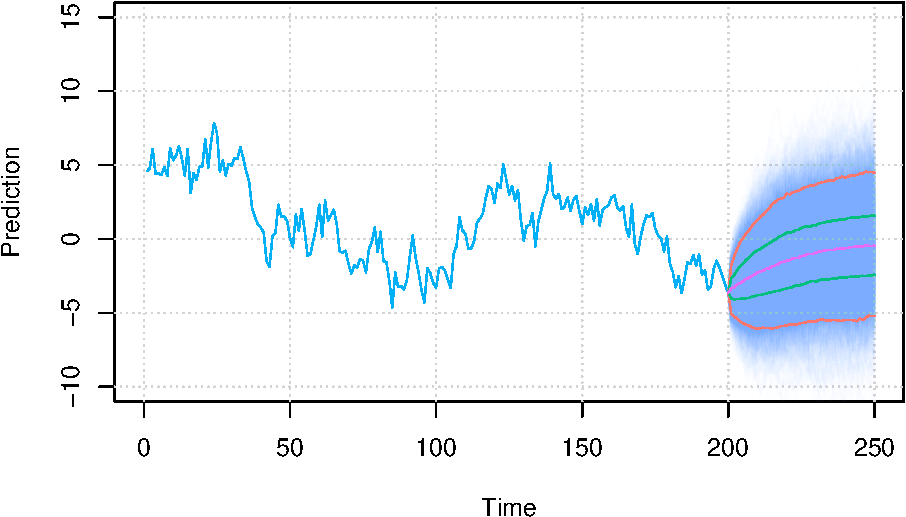
\includegraphics{ts_files/figure-latex/predplot-1.pdf}
\caption{\label{fig:predplot}Values of the AR(2) predictions with the pink
line being the median prediction, red and green lines are respectively
95\% and 75\% Confidence intervals.}
\end{figure}

It can be observed that, as hinted by the expressions for the variance
of the predictions (in the examples above), the variability of the
predictions increases as we try to predict further into the future.

Having now defined the basic concepts for forecasting of time series we
can now start another topic of considerable importance for time series
analysis. Indeed, the whole discussion on prediction is not only
important to derive forecasts for future values of the phenomena one may
be interested in, but also in understanding how well a model explains
(and predicts) an observed time series. In fact, predictions allow to
deliver residuals within the time series setting and, based on these
residuals, we can obtain different inference and diagnostic tools.

Given the knowledge on predictions seen above, residuals can be computed
as

\[r_{t+j} = X_{t+j} - \hat{X}_{t+j},\] where \(\hat{X}_{t+j}\)
represents an estimator of the conditional expectation
\(E[X_{t+j} | \Omega_{t}]\). The latter quantity will depend on the
model underlying the time series and, assuming we know the true model,
we could use the true parameters to obtain a value for this expectation.
However, in an applied setting it is improbable that we know the true
parameters and therefore \(\hat{X}_{t+j}\) can be obtained by estimating
the parameters (as seen in the previous sections) and then plugging
thmem into the expression of \(E[X_{t+j} | \Omega_{t}]\).

\section{Diagnostic Tools for Time
Series}\label{diagnostic-tools-for-time-series}

The standard approach to understanding how well a model fits the data is
analysing the residuals (e.g.~linear regression). The same approach can
be taken for time series analysis where, given our knowledge on
forecasts from the previous section, we can now deliver residuals. The
first step (and possibly the most important) is to use visual tools to
check the residuals and also the original time series. Below is a figure
that collects different diagnostic tools for time series analysis and is
applied to a simulated AR(1) process of length \(T = 100\).

\begin{Shaded}
\begin{Highlighting}[]
\KeywordTok{set.seed}\NormalTok{(}\DecValTok{333}\NormalTok{)}
\NormalTok{true_model =}\StringTok{ }\KeywordTok{AR}\NormalTok{(}\DataTypeTok{phi =} \FloatTok{0.8}\NormalTok{, }\DataTypeTok{sigma2 =} \DecValTok{1}\NormalTok{)}
\NormalTok{Xt =}\StringTok{ }\KeywordTok{gen_gts}\NormalTok{(}\DataTypeTok{n =} \DecValTok{100}\NormalTok{, }\DataTypeTok{model =}\NormalTok{ true_model)}
\NormalTok{model =}\StringTok{ }\KeywordTok{estimate}\NormalTok{(}\KeywordTok{AR}\NormalTok{(}\DecValTok{1}\NormalTok{), Xt, }\DataTypeTok{demean =} \OtherTok{FALSE}\NormalTok{)}
\KeywordTok{check}\NormalTok{(}\DataTypeTok{model =}\NormalTok{ model)}
\end{Highlighting}
\end{Shaded}

\begin{figure}

{\centering \includegraphics{ts_files/figure-latex/diagnostic_plot-1} 

}

\caption{Ljung-Box test p-values for the residuals of the fitted AR(1) model over lags $h = 1, ...., 20$.}(\#fig:diagnostic_plot)
\end{figure}

All plots refer to the residuals of the model-fit and aim at visually
assessing whether the fitted time series model captures the dependence
structure in the data. The first row contains plots that can be
interpreted in the same manner as the residuals from a linear
regression. The first plot simply represents the residuals over time and
should show if there is any presence of trends, seasonality or
heteroskedasticity. The second plot gives a histogram (and smoothed
histrogram called a kernel) of the residuals which should be centered in
zero and (possibly) have an approximate normal distribution. The latter
hypothesis can also be checked using the third plot which consists in a
Normal quantile-quantile plot and the residuals should lie on (or close
to) the diagonal line representing correspondance between the
distributions.

The first plot in the second row in the above figureshows the estimated
ACF. It can be seen how the estimated autocorrelations all lie within
the blue shaded area representing the confidence intervals. The second
plot represents the Partial AutoCorrelation Function (PACF) and is
another tool that will be investigated further on. In the meantime,
suffice it to say that this tool can be interpreted as a different
version of the ACF which measures autocorrelation conditionally on the
previous lags (in some sense, it measures the direct impact of \(X_t\)
on \(X{t+h}\) removing the influence of all observations inbetween). In
this case, we see that also the estimated PACF lies within the
confidence intervals and, along with the intepretation of the ACF, we
can state that the model appears to fit the time series reasonably well
since the residuals can be considered as following a white noise
process. Finally, the last plot visualises the ``Ljung-Box Test'' (which
is a type of Portmanteau test) that tests whether the autocorrelation of
the residuals at a set of lags is different from zero. The plot
represents the p-value of this test at the different lags and also shows
a dashed line representing the common significance level of
\(\alpha = 0.05\). If the modelling has done a good job, all p-values
should be larger than this level. In this case, using the latter level,
we can see that the autocorrelations for the residuals appear to be
non-significant and therefore fitting an AR(1) model to the time series
(which is the true model in this example) appears to do a reasonably
good job.

\subsection{The Partial AutoCorrelation Function
(PACF)}\label{the-partial-autocorrelation-function-pacf}

Before further discussing these diagnostic tools, let us focus a little
more on the PACF mentioned earlier. As briefly highlighted above, this
function measures the degree of linear correlation between two lagged
observations by removing the effect of the observations in the
intermediate lags. For example, let us assume we have three correlated
variables \(X\), \(Y\) and \(Z\) and we wish to find the direct
correlation between \(X\) and \(Y\): we can apply a linear regression of
\(X\) on \(Z\) (to obtain \(\hat{X}\)) and \(Y\) on \(Z\) (to obtain
\(\hat{Y}\)) and thereby compute \(corr(\hat{X}, \hat{Y})\) which
represents the partial autocorrelation. In this manner, the effect of
\(Z\) on the correlation between \(X\) and \(Y\) is removed. Considering
the variables as being indexed by time (i.e.~a time series), we can
therefore define the following quantities
\[\hat{X}_{t+h} = \beta_1 X_{t+h-1} + \beta_2 X_{t+h-2} + ... + \beta_{h-1} X_{t+1},\]
and

\[\hat{X}_{t} = \beta_1 X_{t+1} + \beta_2 X_{t+2} + ... + \beta_{h-1} X_{t+h-1},\]
which represent the regressions of \(X_{t+h}\) and \(X_t\) on all
intermediate observations. With these defintions, let us more formally
define the PACF.

\BeginKnitrBlock{definition}[Partial AutoCorrelation Function]
\protect\hypertarget{def:pacf}{}{\label{def:pacf} \iffalse (Partial
AutoCorrelation Function) \fi{} }The partial autocorrelation function of
a (weakly) stationary time series \((X_t)\) is defined as
\[\rho_{1,1} = \operatorname{corr}(X_{t+1}, X_t) = \rho(1),\] and
\[\rho_{h,h} = \operatorname{corr}((X_{t+h} - \hat{X}_{t+h}), (X_t - \hat{X}_t)), \, h > 1.\]
\EndKnitrBlock{definition}

Therefore, the PACF is not defined at lag zero while it is the same as
the ACF at the first lag since there are no intermediate observations.
The defintion of this function is important for different reasons.
Firstly, as mentioned earlier, we have an asymptotic distribution for
the estimator of the PACF which allows us to deliver confidence
intervals as for the ACF. Indeed, representing the empirical PACF along
with its confidence intervals can provide a further tool to make sure
that the residuals of a model fit can be considered as being white
noise. The latter is a reasonable hypothesis if both the empirical ACF
and PACF lie within the confidence intervals indicating that there is no
significant correlation between lagged variables. Let us focus on the
empirical PACF of the residuals we saw earlier in the diagnostic plot.

\begin{Shaded}
\begin{Highlighting}[]
\NormalTok{residuals =}\StringTok{ }\NormalTok{model}\OperatorTok{$}\NormalTok{mod}\OperatorTok{$}\NormalTok{residuals}
\KeywordTok{plot}\NormalTok{(}\KeywordTok{auto_corr}\NormalTok{(residuals, }\DataTypeTok{pacf =} \OtherTok{TRUE}\NormalTok{))}
\end{Highlighting}
\end{Shaded}

\begin{figure}

{\centering \includegraphics{ts_files/figure-latex/unnamed-chunk-41-1} 

}

\caption{Empirical PACF on the residuals of the AR(1) model fitted to the simulated time series generated from an AR(1) process.}\label{fig:unnamed-chunk-41}
\end{figure}

From the plot we see that the estimated PACF at all lags lies within the
blue shaded area representing the 95\% confidence intervals indicating
that the residuals don't appear to have any form of direct
autocorrelation over lags and, hence, that they can be considered as
white noise. In addition to delivering a tool to analyse the residuals
of a model fit, the PACF is especially useful for diagnostic purposes in
order to detect the possible models that have generated an observed time
series. With respect to the class of models studied this far
(i.e.~AR(\(p\)) models), the PACF can give important insight to the
order of the AR(\(p\)) model, more specifically the value of \(p\).
Indeed, the ACF of an AR(\(p\)) model tends to decrease in a sinusoidal
fashion and exponetially fast to zero as the lag \(h\) increases thereby
giving a hint that the underlying model belongs to the AR(\(p\)) family.
However, aside from hinting to the fact that the model belongs to the
family of AR(\(p\)) models, the latter function tends to be less
informative with respect to which AR(\(p\)) model (i.e.~which value of
\(p\)) is best suited for the observed time series. The PACF on the
other hand is non-zero for the first \(p\) lags and then becomes zero
for \(h > p\), therefore it can give an important indication with
respect to which order should be considered to best model the time
series.

With the above discussion in mind, let us consider some examples where
we study the theoretical ACF and PACF of different AR(\(p\)) models. The
first is an AR(1) model with parameter \(\phi = 0.95\) and its ACF and
PACF are shown below.

\begin{Shaded}
\begin{Highlighting}[]
\KeywordTok{par}\NormalTok{(}\DataTypeTok{mfrow =} \KeywordTok{c}\NormalTok{(}\DecValTok{1}\NormalTok{, }\DecValTok{2}\NormalTok{))}
\KeywordTok{plot}\NormalTok{(}\KeywordTok{theo_acf}\NormalTok{(}\DataTypeTok{ar =} \FloatTok{0.95}\NormalTok{, }\DataTypeTok{ma =} \OtherTok{NULL}\NormalTok{))}
\KeywordTok{plot}\NormalTok{(}\KeywordTok{theo_pacf}\NormalTok{(}\DataTypeTok{ar =} \FloatTok{0.95}\NormalTok{, }\DataTypeTok{ma =} \OtherTok{NULL}\NormalTok{))}
\end{Highlighting}
\end{Shaded}

\begin{figure}

{\centering \includegraphics{ts_files/figure-latex/unnamed-chunk-42-1} 

}

\caption{Theoretical ACF (left) and PACF (right) of an AR(1) model with parameter $\phi = 0.95$.}\label{fig:unnamed-chunk-42}
\end{figure}

We can see that the ACF decreases exponentially fast as we would expect
for an AR(p) model while the PACF has the same values of the ACF at lag
1 (which is always the case) and is zero for \(h > 1\). The latter
therefore indicates the order \(p\) of the AR(\(p\)) model which in this
case is \(p=1\). Let us now consider the following models as further
examples:

\[X_t = 0.5 X_{t-1} + 0.25 X_{t-2} + 0.125 X_{t-3} + W_t\]

and

\[X_t = -0.1 X_{t-2} -0.1 X_{t-4} + 0.6 X_{t-5} + W_t.\]

The first model is an AR(3) model with positive coefficients while the
second is an AR(5) model where \(\phi_1 = \phi_3 = 0\). The ACF and PACF
of the first AR(3) model is shown below.

\begin{Shaded}
\begin{Highlighting}[]
\KeywordTok{par}\NormalTok{(}\DataTypeTok{mfrow =} \KeywordTok{c}\NormalTok{(}\DecValTok{1}\NormalTok{, }\DecValTok{2}\NormalTok{))}
\KeywordTok{plot}\NormalTok{(}\KeywordTok{theo_acf}\NormalTok{(}\DataTypeTok{ar =} \KeywordTok{c}\NormalTok{(}\FloatTok{0.5}\NormalTok{, }\FloatTok{0.25}\NormalTok{, }\FloatTok{0.125}\NormalTok{), }\DataTypeTok{ma =} \OtherTok{NULL}\NormalTok{))}
\KeywordTok{plot}\NormalTok{(}\KeywordTok{theo_pacf}\NormalTok{(}\DataTypeTok{ar =} \KeywordTok{c}\NormalTok{(}\FloatTok{0.5}\NormalTok{, }\FloatTok{0.25}\NormalTok{, }\FloatTok{0.125}\NormalTok{), }\DataTypeTok{ma =} \OtherTok{NULL}\NormalTok{))}
\end{Highlighting}
\end{Shaded}

\begin{figure}

{\centering \includegraphics{ts_files/figure-latex/unnamed-chunk-43-1} 

}

\caption{Theoretical ACF (left) and PACF (right) of an AR(3) model with parameters $\phi_1 = 0.95$, $\phi_2 = 0.25$ and $\phi_3 = 0.125$.}\label{fig:unnamed-chunk-43}
\end{figure}

Again, we see that the ACF decreases exponentially and also the PACF
plot shows a steady decrease until it becomes zero for \(h > 3\). This
is because the values of \(\phi_i\) are all positive and decreasing as
well. Let us now consider the second model (the AR(5) model) whose ACF
and PACF plots are represented below.

\begin{Shaded}
\begin{Highlighting}[]
\KeywordTok{par}\NormalTok{(}\DataTypeTok{mfrow =} \KeywordTok{c}\NormalTok{(}\DecValTok{1}\NormalTok{, }\DecValTok{2}\NormalTok{))}
\KeywordTok{plot}\NormalTok{(}\KeywordTok{theo_acf}\NormalTok{(}\DataTypeTok{ar =} \KeywordTok{c}\NormalTok{(}\DecValTok{0}\NormalTok{, }\OperatorTok{-}\FloatTok{0.1}\NormalTok{, }\DecValTok{0}\NormalTok{, }\OperatorTok{-}\FloatTok{0.1}\NormalTok{, }\FloatTok{0.6}\NormalTok{), }\DataTypeTok{ma =} \OtherTok{NULL}\NormalTok{))}
\KeywordTok{plot}\NormalTok{(}\KeywordTok{theo_pacf}\NormalTok{(}\DataTypeTok{ar =} \KeywordTok{c}\NormalTok{(}\DecValTok{0}\NormalTok{, }\OperatorTok{-}\FloatTok{0.1}\NormalTok{, }\DecValTok{0}\NormalTok{, }\OperatorTok{-}\FloatTok{0.1}\NormalTok{, }\FloatTok{0.6}\NormalTok{), }\DataTypeTok{ma =} \OtherTok{NULL}\NormalTok{))}
\end{Highlighting}
\end{Shaded}

\begin{figure}

{\centering \includegraphics{ts_files/figure-latex/unnamed-chunk-44-1} 

}

\caption{Theoretical ACF (left) and PACF (right) of an AR(4) model with parameters $\phi_1 = 0$, $\phi_2 = -0.1$, $\phi_3 = 0$ and $\phi_4 = 0$.}\label{fig:unnamed-chunk-44}
\end{figure}

In this case we see that the ACF has a sinusoidal-like behaviour where
the values of \(\phi_1 = \phi_3 = 0\) and the negative
\(\phi_2 = \phi_4 = -0.1\) values deliver this alternating ACF form
which nevertheless decreases as \(h\) increases. These values deliver
the PACF plot on the right which is negative for the first lags and is
greatly positive at \(h=5\) only to become zero for \(h > 5\).

These examples therefore give us further insight as to how to interpret
the empirical (or estimated) versions of these functions. For this
reason, let us study the empirical ACF and PACF of some real time
series, the first of which is the data representing the natural
logarithm of the annual number of Lynx trappings in Canada between 1821
and 1934. The time series is represented below.

\begin{Shaded}
\begin{Highlighting}[]
\NormalTok{lynx_gts =}\StringTok{ }\KeywordTok{gts}\NormalTok{(}\KeywordTok{log}\NormalTok{(lynx), }\DataTypeTok{start =} \DecValTok{1821}\NormalTok{, }\DataTypeTok{data_name =} \StringTok{"Lynx Trappings"}\NormalTok{, }\DataTypeTok{unit_time =} \StringTok{"year"}\NormalTok{, }\DataTypeTok{name_ts =} \StringTok{"Trappings"}\NormalTok{)}
\KeywordTok{plot}\NormalTok{(lynx_gts)}
\end{Highlighting}
\end{Shaded}

\begin{figure}

{\centering \includegraphics{ts_files/figure-latex/unnamed-chunk-46-1} 

}

\caption{Time series of annual number of lynx data trappings in Canada between 1821 and 1934.}\label{fig:unnamed-chunk-46}
\end{figure}

We can see that there appears to be a seasonal trend within the data but
let us ignore this for the moment and check the ACF and PACF plots
below.

\begin{Shaded}
\begin{Highlighting}[]
\KeywordTok{corr_analysis}\NormalTok{(lynx_gts)}
\end{Highlighting}
\end{Shaded}

\begin{figure}

{\centering \includegraphics{ts_files/figure-latex/unnamed-chunk-47-1} 

}

\caption{Empirical ACF (left) and PACF (right) of the lynx time series data.}\label{fig:unnamed-chunk-47}
\end{figure}

The seasonal behaviour also appears in the ACF plot but we see that it
decreases in a sinusoidal fashion as the lag increases hinting that an
AR(p) model could be a potential candidate for the time series. Looking
at the PACF plot on the right we can see that a few partial
autocorrelations appear to be significant up to lag \(h=11\). Therefore
an AR(11) model could be a possibly good candidate to explain (and
predict) this time series.

\subsection{Portmanteau Tests}\label{portmanteau-tests}

In a similar manner to using the ACF and PACF confidence intervals to
understand if the residuals can be considered as white noise, other
statistical tests exist to determine if the autocorrelations can be
considered as being significant or not. Indeed, the 95\% confidence
intervals can be extremely useful in detecting significant (partial)
autocorrelations but they cannot be considered as an overall test for
white noise since (aside from being asymptotic and therefore
approximate) they do not consider the multiple testing hypothesis
implied by them (i.e.~if we're testing all lags, the actual level of
significance should be modified in order to bound type I errors). For
this reason, Portmanteau tests have been proposed in order to deliver an
overall test that jointly considers a set of lags and determines whether
their autocorrelation is significantly different from zero (i.e.~whether
the residuals can be considered white noise or not).

One of the most popular Portmanteau tests is the Ljung-Box test whose
statistic is defined as follows:

\[Q_h = T(T+2) \sum_{j=1}^{h} \frac{\hat{\rho}_j^2}{T - j},\] where
\(h\) represents the maximum lag of the set of lags for which we wish to
test for serial autocorrelation (i.e.~from lag 1 to lag \(h\)). Under
the null hypothesis \(Q_h \sim \chi_h^2\) since asymptotically
\(\hat{\rho}_j \sim \mathcal{N}\left(0, \frac{1}{T}\right)\) under the
null and therefore the statistic is proportional to the sum of squared
standard normal variables. The last plot of Figure
@ref(fig:diagnostic\_plot) can therefore be better interpreted under
this framework and is reproduced below.

\begin{Shaded}
\begin{Highlighting}[]
\NormalTok{lb_test =}\StringTok{ }\KeywordTok{diag_ljungbox}\NormalTok{(}\KeywordTok{as.numeric}\NormalTok{(residuals), }\DataTypeTok{order =} \DecValTok{0}\NormalTok{, }\DataTypeTok{stop_lag =} \DecValTok{20}\NormalTok{, }\DataTypeTok{stdres =} \OtherTok{FALSE}\NormalTok{, }\DataTypeTok{plot =} \OtherTok{TRUE}\NormalTok{)}
\end{Highlighting}
\end{Shaded}

\begin{figure}

{\centering \includegraphics{ts_files/figure-latex/unnamed-chunk-49-1} 

}

\caption{Ljung-Box p-values for lags $h = 1,...,20$ on the residuals of the fitted AR(1) model.}\label{fig:unnamed-chunk-49}
\end{figure}

Each p-value represented in the plot above is therefore the p-value for
the considered maximum lag. Therefore the first p-value (at lag 1) is
the p-value for the null hypothesis that all lags up to lag 1 are equal
to zero, the second is for the null hypothesis that all lags up to lag 2
are equal to zero and so on. Hence, each p-value represents a global
test on the autocorrelations up to the considered maximum lag \(h\) and
delivers additional information regarding the dependence structure
within the residuals. In this case, as interpreted earlier, all p-values
are larger than the \(\alpha = 0.05\) level and is an additional
indication that the residuals follow a white noise process (and that the
fitted model appears to well describe the observed time series).

There are other Portmanteau tests with different advantages (and
disadvantages) over the Ljung-Box test but these are beyond the scope of
this textbook.

\section{Inference for AR(p) Models}\label{inference-for-arp-models}

For all the above methods, it would be necessary to understand how
``precise'' their estimates are. To do so we would need to obtain
confidence intervals for these estimates and this can be done mainly in
two manners:

\begin{itemize}
\tightlist
\item
  using the asymptotic distribution of the parameter estimates;
\item
  using parametric bootstrap.
\end{itemize}

The first approach consists in using the asymptotic distribution of the
estimators presented earlier to deliver approximations of the confidence
intervals which get better as the length of the observed time series
increases. Hence, if for example we wanted to find a 95\% confidence
interval for the parameter \(\phi\), we would use the quantiles of the
normal distribution (given that all methods presented earlier present
this asymptotic distribution). However, this approach can present some
drawbacks, one of which its behaviour when the parameters are close to
the boundaries of the parameter space. Suppose we consider a realization
of length \(T = 100\) of the following AR(1) model:

\[X_t = 0.96 X_{t-1} + W_t, \;\;\;\; W_t \sim \mathcal{N}(0,1),\]

which is represented in Figure \ref{fig:simAR1ci}

\begin{Shaded}
\begin{Highlighting}[]
\KeywordTok{set.seed}\NormalTok{(}\DecValTok{55}\NormalTok{)}
\NormalTok{x =}\StringTok{ }\KeywordTok{gen_gts}\NormalTok{(}\DataTypeTok{n =} \DecValTok{100}\NormalTok{, }\KeywordTok{AR1}\NormalTok{(}\FloatTok{0.96}\NormalTok{, }\DecValTok{1}\NormalTok{))}
\KeywordTok{plot}\NormalTok{(x)}
\end{Highlighting}
\end{Shaded}

\begin{figure}

{\centering \includegraphics{ts_files/figure-latex/simAR1ci-1} 

}

\caption{AR(1) with $\phi$ close to parameter bound}\label{fig:simAR1ci}
\end{figure}

It can be seen that the parameter \(\phi = 0.96\) respects the condition
for stationarity (i.e.\(\left| \phi \right| < 1\)) but is very close to
its boundary. Using the MLE, we first estimate the parameters and then
compute confidence intervals for \(\phi\) using the asymptotic normal
distribution.

\begin{Shaded}
\begin{Highlighting}[]
\CommentTok{# Compute the parameter estimates using MLE}
\NormalTok{fit.ML =}\StringTok{ }\KeywordTok{estimate}\NormalTok{(}\KeywordTok{AR}\NormalTok{(}\DecValTok{1}\NormalTok{), x, }\DataTypeTok{demean =} \OtherTok{FALSE}\NormalTok{)}
\KeywordTok{c}\NormalTok{(}\StringTok{"phi"}\NormalTok{ =}\StringTok{ }\NormalTok{fit.ML}\OperatorTok{$}\NormalTok{mod}\OperatorTok{$}\NormalTok{coef[}\DecValTok{1}\NormalTok{], }\StringTok{"sigma2"}\NormalTok{ =}\StringTok{ }\KeywordTok{sqrt}\NormalTok{(fit.ML}\OperatorTok{$}\NormalTok{mod}\OperatorTok{$}\NormalTok{sigma2))}
\end{Highlighting}
\end{Shaded}

\begin{verbatim}
##   phi.ar1    sigma2 
## 0.9206575 0.9449144
\end{verbatim}

\begin{Shaded}
\begin{Highlighting}[]
\CommentTok{# Construct asymptotic confidence interval for phi}
\NormalTok{fit.ML}\OperatorTok{$}\NormalTok{mod}\OperatorTok{$}\NormalTok{coef[}\DecValTok{1}\NormalTok{] }\OperatorTok{+}\StringTok{ }\KeywordTok{c}\NormalTok{(}\OperatorTok{-}\DecValTok{1}\NormalTok{,}\DecValTok{1}\NormalTok{)}\OperatorTok{*}\FloatTok{1.96}\OperatorTok{*}\KeywordTok{as.numeric}\NormalTok{(}\KeywordTok{sqrt}\NormalTok{(fit.ML}\OperatorTok{$}\NormalTok{mod}\OperatorTok{$}\NormalTok{var.coef))}
\end{Highlighting}
\end{Shaded}

\begin{verbatim}
## [1] 0.8479738 0.9933412
\end{verbatim}

\begin{verbatim}
## Fitted model: AR(1)
## 
## Estimated parameters:
## Model Information: 
##        Estimates
## AR     0.9700676
## SIGMA2 0.9526867
## 
## * The initial values of the parameters used in the minimization of the GMWM objective function 
##   were generated by the program underneath seed: 1337. 
## 
## 95 % confidence intervals:
##        Estimates    CI Low  CI High         SE
## AR     0.9700676 0.8028770 1.048532 0.07467374
## SIGMA2 0.9526867 0.7132915 1.206341 0.14987655
\end{verbatim}

From the estimation summary, we can notice that the MLE confidence
intervals contain values that would make the AR(1) non-stationary
(i.e.~values of \(\phi\) larger than 1). However, these confidence
intervals are based on the (asymptotic) distributions of \(\hat{\phi}\)
which are shown in Figure \ref{fig:asymIC} along with those based on the
GMWM estimator.

\begin{figure}
\centering
\includegraphics{ts_files/figure-latex/asymIC-1.pdf}
\caption{\label{fig:asymIC}Estimated asymptotic distribution of
\(\hat{\phi}\) for MLE and GMWM parameter estimates. The dashed vertical
line represents the true value of \(\phi\), the solid line denotes the
upper bound of the parameter space for \(\phi\) and the vertical ticks
represent the limits of the 95\% confidence intervals for both methods.}
\end{figure}

Therefore, if we estimate a stationary AR(1) model, it would be
convenient to have more ``realistic'' confidence intervals that give
limits for a stationary AR(1) model. A viable solution for this purpose
is to use parametric bootstrap. Indeed, parametric bootstrap takes the
estimated parameter values and uses them in order to simulate from the
assumed model (an AR(1) process in this case). For each simulation, the
parameters are estimated and stored in order to obtain an empirical
(finite sample) distribution of the estimators. Based on this
distribution it is consequently possible to find the \(\alpha/2\) and
\(1-\alpha/2\) empirical quantiles thereby delivering confidence
intervals that should not suffer from boundary problems (since the
estimation procedure looks for solutions within the admissable regions).
The code below gives an example of how this confidence interval is built
based on the same estimation procedure but using parametric bootstrap
(using \(B = 10,000\) bootstrap replicates).

\begin{Shaded}
\begin{Highlighting}[]
\CommentTok{# Number of Iterations}
\NormalTok{B =}\StringTok{ }\DecValTok{10000}

\CommentTok{# Set up storage for results}
\NormalTok{est.phi.gmwm =}\StringTok{ }\KeywordTok{rep}\NormalTok{(}\OtherTok{NA}\NormalTok{,B)}
\NormalTok{est.phi.ML =}\StringTok{ }\KeywordTok{rep}\NormalTok{(}\OtherTok{NA}\NormalTok{,B)}

\CommentTok{# Model generation statements}
\NormalTok{model.gmwm =}\StringTok{ }\KeywordTok{AR}\NormalTok{(}\DataTypeTok{phi =} \KeywordTok{c}\NormalTok{(fit.gmwm}\OperatorTok{$}\NormalTok{mod}\OperatorTok{$}\NormalTok{estimate[}\DecValTok{1}\NormalTok{]), }\DataTypeTok{sigma2 =} \KeywordTok{c}\NormalTok{(fit.gmwm}\OperatorTok{$}\NormalTok{mod}\OperatorTok{$}\NormalTok{estimate[}\DecValTok{2}\NormalTok{]))}
\NormalTok{model.mle =}\StringTok{ }\KeywordTok{AR}\NormalTok{(}\DataTypeTok{phi =} \KeywordTok{c}\NormalTok{(fit.ML}\OperatorTok{$}\NormalTok{mod}\OperatorTok{$}\NormalTok{coef), }\DataTypeTok{sigma2 =} \KeywordTok{c}\NormalTok{(fit.ML}\OperatorTok{$}\NormalTok{mod}\OperatorTok{$}\NormalTok{sigma2))}

\CommentTok{# Begin bootstrap}
\ControlFlowTok{for}\NormalTok{(i }\ControlFlowTok{in} \KeywordTok{seq_len}\NormalTok{(B))\{}

  \CommentTok{# Set seed for reproducibility}
  \KeywordTok{set.seed}\NormalTok{(B }\OperatorTok{+}\StringTok{ }\NormalTok{i)}

  \CommentTok{# Generate process under MLE parameter estimate}
\NormalTok{  x.star =}\StringTok{ }\KeywordTok{gen_gts}\NormalTok{(}\DecValTok{100}\NormalTok{, model.mle)}

  \CommentTok{# Attempt to estimate phi by employing a try}
\NormalTok{  est.phi.ML[i] =}\StringTok{ }\KeywordTok{tryCatch}\NormalTok{(}\KeywordTok{estimate}\NormalTok{(}\KeywordTok{AR}\NormalTok{(}\DecValTok{1}\NormalTok{), x.star, }\DataTypeTok{demean =} \OtherTok{FALSE}\NormalTok{)}\OperatorTok{$}\NormalTok{mod}\OperatorTok{$}\NormalTok{coef,}
                           \DataTypeTok{error =} \ControlFlowTok{function}\NormalTok{(e) }\OtherTok{NA}\NormalTok{)}

  \CommentTok{# Generate process under GMWM parameter estimate}
\NormalTok{  x.star =}\StringTok{ }\KeywordTok{gen_gts}\NormalTok{(}\DecValTok{100}\NormalTok{, model.gmwm)}
\NormalTok{  est.phi.gmwm[i] =}\StringTok{ }\KeywordTok{estimate}\NormalTok{(}\KeywordTok{AR}\NormalTok{(}\DecValTok{1}\NormalTok{), x.star, }\DataTypeTok{method =} \StringTok{"gmwm"}\NormalTok{)}\OperatorTok{$}\NormalTok{mod}\OperatorTok{$}\NormalTok{estimate[}\DecValTok{1}\NormalTok{]}
\NormalTok{\}}
\end{Highlighting}
\end{Shaded}

\begin{figure}
\centering
\includegraphics{ts_files/figure-latex/paraAR1cigraphs-1.pdf}
\caption{\label{fig:paraAR1cigraphs}Parametric bootstrap distributions of
\(\hat{\phi}\) for the MLE and GMWM parameter estimates. The histograms
represent the empirical distributions resulting from the parametric
bootstrap while the continuous densities represent the estimated
asymptotic distributions. The vertical line represents the true value of
\(\phi\), the dark solid lines represent the upper bound of the
parameter space for \(\phi\) and the vertical ticks represent the limits
of the 95\% confidence intervals for the asymptotic distributions (red
and gold) and the empirical distributions (green and blue).}
\end{figure}

In Figure \ref{fig:paraAR1cigraphs}, we compare the estimated densities
for \(\hat{\phi}\) using asymptotic results and bootstrap techniques for
the MLE and the GMWM estimators. It can be observed that the issue that
arose previously with ``non-stationary'' confidence intervals does not
occur with the parametric bootstrap approach since the interval regions
of the latter lie entirely within the boundaries of the admissable
parameter space.

To further emphasize the advantages of parametric bootstrap, let us
consider one additonal example of an AR(2) process. For this example,
discussion will focus solely on the behaviour of the MLE. Having said
this, the considered AR(2) process is defined as follows:

\begin{equation}
{X_t} = {1.98}{X_{t - 1}} - {0.99}{X_{t - 2}} + {W_t}
\label{eq:ciar2}
\end{equation}

where \(W_t \sim \mathcal{N}(0, 1)\). The generated process is displayed
in Figure \ref{fig:CIAR2data}.

\begin{Shaded}
\begin{Highlighting}[]
\KeywordTok{set.seed}\NormalTok{(}\DecValTok{432}\NormalTok{)}
\NormalTok{Xt =}\StringTok{ }\KeywordTok{gen_gts}\NormalTok{(}\DecValTok{500}\NormalTok{, }\KeywordTok{AR}\NormalTok{(}\DataTypeTok{phi =} \KeywordTok{c}\NormalTok{(}\FloatTok{1.98}\NormalTok{, }\OperatorTok{-}\FloatTok{0.99}\NormalTok{), }\DataTypeTok{sigma2 =} \DecValTok{1}\NormalTok{))}
\KeywordTok{plot}\NormalTok{(Xt)}
\end{Highlighting}
\end{Shaded}

\begin{figure}

{\centering \includegraphics{ts_files/figure-latex/CIAR2data-1} 

}

\caption{Generated AR(2) Process}\label{fig:CIAR2data}
\end{figure}

\begin{Shaded}
\begin{Highlighting}[]
\NormalTok{fit =}\StringTok{ }\KeywordTok{estimate}\NormalTok{(}\KeywordTok{AR}\NormalTok{(}\DecValTok{2}\NormalTok{), Xt, }\DataTypeTok{demean =} \OtherTok{FALSE}\NormalTok{)}
\NormalTok{fit}
\end{Highlighting}
\end{Shaded}

\begin{verbatim}
## Fitted model: AR(2)
## 
## Estimated parameters:
## 
## Call:
## arima(x = as.numeric(Xt), order = c(p, intergrated, q), seasonal = list(order = c(P, 
##     seasonal_intergrated, Q), period = s), include.mean = demean, method = meth)
## 
## Coefficients:
##          ar1      ar2
##       1.9787  -0.9892
## s.e.  0.0053   0.0052
## 
## sigma^2 estimated as 0.8419:  log likelihood = -672.58,  aic = 1351.15
\end{verbatim}

Having estimated the model's coefficients, we can again perform the
parametric bootstrap. It must be noticed that in these simulations there
can be various cases where a method may fail to estimate due to
numerical issues (e.g.~numerically singular covariance matrices, etc.)
and therefore we add a check for each estimation to ensure that we
preserve those estimations that have succeeded.

\begin{Shaded}
\begin{Highlighting}[]
\NormalTok{B =}\StringTok{ }\DecValTok{500}
\NormalTok{est.phi.ML =}\StringTok{ }\KeywordTok{matrix}\NormalTok{(}\OtherTok{NA}\NormalTok{, B, }\DecValTok{2}\NormalTok{)}
\NormalTok{model =}\StringTok{ }\KeywordTok{AR}\NormalTok{(}\DataTypeTok{phi =}\NormalTok{ fit}\OperatorTok{$}\NormalTok{mod}\OperatorTok{$}\NormalTok{coef, }\DataTypeTok{sigma2 =}\NormalTok{ fit}\OperatorTok{$}\NormalTok{mod}\OperatorTok{$}\NormalTok{sigma2)}

\ControlFlowTok{for}\NormalTok{(i }\ControlFlowTok{in} \KeywordTok{seq_len}\NormalTok{(B)) \{}
  \KeywordTok{set.seed}\NormalTok{(B }\OperatorTok{+}\StringTok{ }\NormalTok{i)              }\CommentTok{# Set Seed for reproducibilty}
\NormalTok{  x.star =}\StringTok{ }\KeywordTok{gen_gts}\NormalTok{(}\DecValTok{500}\NormalTok{, model) }\CommentTok{# Simulate the process}

  \CommentTok{# Obtain parameter estimate with protection}
  \CommentTok{# that defaults to NA if unable to estimate}
\NormalTok{  est.phi.ML[i,] =}\StringTok{ }\KeywordTok{tryCatch}\NormalTok{(}\KeywordTok{estimate}\NormalTok{(}\KeywordTok{AR}\NormalTok{(}\DecValTok{2}\NormalTok{), x.star, }\DataTypeTok{demean =} \OtherTok{FALSE}\NormalTok{)}\OperatorTok{$}\NormalTok{mod}\OperatorTok{$}\NormalTok{coef,}
  \DataTypeTok{error =} \ControlFlowTok{function}\NormalTok{(e) }\OtherTok{NA}\NormalTok{)}
\NormalTok{\}}
\end{Highlighting}
\end{Shaded}

Once this is done, we can compare the bivariate distributions
(asymptotic and bootsrapped) of the two estimated parameters
\(\hat{\phi}_1\) and \(\hat{\phi}_2\).

\begin{figure}
\centering
\includegraphics{ts_files/figure-latex/ciAR2d-1.pdf}
\caption{\label{fig:ciAR2d}Estimated distributions of \(\hat{\phi_1}\) and
\(\hat{\phi_2}\) based on the MLE using asymptotic and parametric
bootstrap techniques. The colored contours represent the density of the
distributions and the dark grey lines represent the boundary constraints
of \(\left|\phi_2\right|<1\) and \(\phi_2 = 1 - \phi_1\).}
\end{figure}

As for any other estimation and inference procedure, these confidence
intervals rely on the assumption that the chosen model (AR(2) in this
case) is the true model underlying the observed time series. However, if
this assumption were not correct, then the derived confidence intervals
would not be correct and this could possibly lead to bad conclusions.
For this reason, one could decide to use a non-parametric approach to
computing these confidence intervals, such as the traditional bootstrap
that consists in a simple random sampling with replacement from the
original data. However, this approach would not be appropriate in the
presence of dependence between observations since this procedure would
break the dependence structure and therefore deliver unreliable
conclusions. Therefore, to preserve the dependence structure of the
original data one option would be to use \emph{block bootstrapping},
which is a particular form of non-parametric bootstrap. There are many
different kinds of block-bootstrap procedures for time series which are
all related to the Moving Block Bootstrap (MBB) which is defined as
follows.

\BeginKnitrBlock{definition}
\protect\hypertarget{def:mbb}{}{\label{def:mbb} }Suppose that
\(\left(X_t\right)\) is a weakly stationary time series with \(T\)
observations. The procedure is as follows:

\begin{enumerate}
\def\labelenumi{\arabic{enumi}.}
\tightlist
\item
  Divide the time series into overlapping blocks
  \(\left\{S_1, \ldots, S_M\right\}\) of length \(\ell\),
  \(1 \le \ell < N\), resulting in \(M = N - \ell + 1\) blocks
  structured as:
\end{enumerate}

\[\begin{aligned}
  {S_1}& = & ({X_1}, &{X_2}, \cdots , {X_\ell}) & && \\
  {S_2}& = & &( {X_2}, {X_3}, \cdots , {X_{\ell + 1}}) & && \\
  & \cdots & & {} & \cdots && \\
  {S_M} & = & & & {} &&( {X_{N-\ell+1}}, {X_{N-\ell+2}}, \cdots , {X_{N}})
  \end{aligned}\]

\begin{enumerate}
\def\labelenumi{\arabic{enumi}.}
\setcounter{enumi}{1}
\tightlist
\item
  Draw \(M = \left\lfloor {\frac{N}{\ell}} \right\rfloor\) blocks with
  replacement from these \(\left\{S_1, \ldots, S_M\right\}\) blocks and
  place them in order to form \((X_t^*)\).
\item
  Compute the statistic of interest on the simulated sample \((X_t^*)\).
\item
  Repeat Steps 2 and 3 \(B\) times where \(B\) is sufficiently ``large''
  (typically \(100 \leq B \leq 10,000\)).
\item
  Compute the empirical mean and variance on the statistic of interest
  based on the \(B\) independent replications.

  \EndKnitrBlock{definition}
\end{enumerate}

The approach taken by MBB ensures that within each block the dependency
between observations is preserved. However, one particular issue that
now arises is that some inaccuracy is introduced as a result of
successive blocks potentially being independent from each other. In
reality, this is one of the trade-offs of the MBB approach that can be
mitigated by selecting an optimal \(\ell\) (to improve the accuracy of
the procedure one should choose \(\ell = T^{1/3}\) as \(T \to \infty\)
as being the optimal choice). An earlier variant of MBB is called the
Nonoverlapping Block Bootstrap (NBB) which doesn't allow the blocks to
share common data points and is presented below.

\BeginKnitrBlock{definition}
\protect\hypertarget{def:nbb}{}{\label{def:nbb} }Suppose that
\(\left(X_t\right)\) is weakly stationary time series with \(T\)
observations.

\begin{enumerate}
\def\labelenumi{\arabic{enumi}.}
\tightlist
\item
  Divide time series into nonoverlapping blocks
  \(\left\{S_1, \ldots, S_M\right\}\) of length \(\ell\),
  \(1 \le \ell < N\), resulting in
  \(M = \left\lfloor {\frac{N}{\ell}} \right\rfloor\) blocks structured
  as:
\end{enumerate}

\[\begin{aligned}
  {S_1}& =  ({X_1}, {X_2}, \cdots , {X_\ell})& & && \\
  {S_2}& =  &( {X_{\ell+1}}, {X_{\ell+2}}, \cdots , {X_{2\ell}}) & && \\
  & \cdots  & {} & \cdots && \\
  {S_K} & =  & & {} &&( {X_{\left({N-\ell+1}\right)}}, {X_{N-\ell+2}}, \cdots , {X_{N}})
  \end{aligned}\]

\begin{enumerate}
\def\labelenumi{\arabic{enumi}.}
\setcounter{enumi}{1}
\tightlist
\item
  Draw \(M\) blocks with replacement from these
  \(\left\{S_1, \ldots, S_M\right\}\) blocks and place them in order to
  form \((X_t^*)\).
\item
  Compute the statistic of interest on the simulated sample \((X_t^*)\).
\item
  Repeat Steps 2 and 3 \(B\) times where \(B\) is sufficiently ``large''
  (typically \(100 \leq B \leq 10,000\)).
\item
  Compute the empirical mean and variance on the statistic of interest
  based on the \(B\) independent replications.

  \EndKnitrBlock{definition}
\end{enumerate}

Alternatively, depending on the case one can also use modifications of
the MBB that seeks to change how the beginning and end of the time
series is weighted such as a Circular Block-Bootstrap (CBB) or a
Stationary Bootstrap (SB). The code below implements the MMB to obtain a
bootrstrap distribution for the estimated parameters of an AR(1) model.

\begin{Shaded}
\begin{Highlighting}[]
\NormalTok{ar1_blockboot =}\StringTok{ }\ControlFlowTok{function}\NormalTok{(Xt, }\DataTypeTok{block_len =} \DecValTok{10}\NormalTok{, }\DataTypeTok{B =} \DecValTok{500}\NormalTok{) \{}
\NormalTok{  n =}\StringTok{ }\KeywordTok{length}\NormalTok{(Xt)            }\CommentTok{# Length of Time Series}
\NormalTok{  res =}\StringTok{ }\KeywordTok{rep}\NormalTok{(}\OtherTok{NA}\NormalTok{, B)          }\CommentTok{# Bootstrapped Statistics}
\NormalTok{  m =}\StringTok{ }\KeywordTok{floor}\NormalTok{(n}\OperatorTok{/}\NormalTok{block_len)    }\CommentTok{# Amount of Blocks}

  \ControlFlowTok{for}\NormalTok{ (i }\ControlFlowTok{in} \KeywordTok{seq_len}\NormalTok{(B)) \{   }\CommentTok{# Begin MMB}
    \KeywordTok{set.seed}\NormalTok{(i }\OperatorTok{+}\StringTok{ }\DecValTok{1199}\NormalTok{)      }\CommentTok{# Set seed for reproducibility}
\NormalTok{    x_star =}\StringTok{ }\KeywordTok{rep}\NormalTok{(}\OtherTok{NA}\NormalTok{, n)     }\CommentTok{# Setup storage for new TS}

    \ControlFlowTok{for}\NormalTok{ (j }\ControlFlowTok{in} \KeywordTok{seq_len}\NormalTok{(m)) \{ }\CommentTok{# Simulate new time series}
\NormalTok{      index =}\StringTok{ }\KeywordTok{sample}\NormalTok{(m, }\DecValTok{1}\NormalTok{)  }\CommentTok{# Randomize block starting points}
      \CommentTok{# Place block into time series}
\NormalTok{      x_star[(block_len}\OperatorTok{*}\NormalTok{(j }\OperatorTok{-}\StringTok{ }\DecValTok{1}\NormalTok{) }\OperatorTok{+}\StringTok{ }\DecValTok{1}\NormalTok{)}\OperatorTok{:}\NormalTok{(block_len}\OperatorTok{*}\NormalTok{j)] =}
\StringTok{      }\NormalTok{Xt[(block_len}\OperatorTok{*}\NormalTok{(index }\OperatorTok{-}\StringTok{ }\DecValTok{1}\NormalTok{) }\OperatorTok{+}\StringTok{ }\DecValTok{1}\NormalTok{)}\OperatorTok{:}\NormalTok{(block_len}\OperatorTok{*}\NormalTok{index)]}
\NormalTok{    \}}
    
  \CommentTok{# Calculate parameters with protection}
\NormalTok{  res[i] =}\StringTok{ }\KeywordTok{tryCatch}\NormalTok{(}\KeywordTok{estimate}\NormalTok{(}\KeywordTok{AR}\NormalTok{(}\DecValTok{1}\NormalTok{), x_star, }\DataTypeTok{demean =} \OtherTok{FALSE}\NormalTok{)}\OperatorTok{$}\NormalTok{mod}\OperatorTok{$}\NormalTok{coef,}
  \DataTypeTok{error =} \ControlFlowTok{function}\NormalTok{(e) }\OtherTok{NA}\NormalTok{)}
\NormalTok{  \}}
  \KeywordTok{na.omit}\NormalTok{(res)              }\CommentTok{# Deliver results}
\NormalTok{\}}
\end{Highlighting}
\end{Shaded}

Having defined the function above, let us consider a scenario where the
model's assumptions are not respected (i.e.~wrong model and/or
non-Gaussian time series). Consider an AR(1) and an AR(2) process with
the same coefficients for the first lagged variable (i.e.
\(\phi = \phi_1 = 0.5\)) but with different innovation noise generation
procedures:

\[
    \begin{aligned}
  \mathcal{M}_1:&{}& X_t &=0.5 X_{t-1} + W_t,&{}& W_t\sim \mathcal{N} (0,1) \\
  \mathcal{M}_2:&{}& X_t &=0.5 X_{t-1} + 0.25 X_{t-2} + V_t,&{}& V_t\sim t_4
  \end{aligned}
\]

where \(t_4\) represents the Student-\(t\) distribution with 4 degrees
of freedom (heavy tails). For the first model (\(\mathcal{M}_1\)) we
will use the \texttt{gen\_gts()} function while for the second model
\(\mathcal{M}_2\) we will make use the \texttt{arima.sim()} function in
which we can assign a vector of innovations from a \(t\) distribution.

\begin{Shaded}
\begin{Highlighting}[]
\KeywordTok{set.seed}\NormalTok{(}\DecValTok{1}\NormalTok{)         }\CommentTok{# Set seed for reproducibilty}
\NormalTok{n =}\StringTok{ }\DecValTok{300}             \CommentTok{# Sample size}
\NormalTok{xt_m1 =}\StringTok{ }\KeywordTok{gen_gts}\NormalTok{(n, }\KeywordTok{AR1}\NormalTok{(}\DataTypeTok{phi =} \FloatTok{0.5}\NormalTok{, }\DataTypeTok{sigma2 =} \DecValTok{1}\NormalTok{))   }\CommentTok{# Gaussian noise only}
\NormalTok{xt_m2 =}\StringTok{ }\KeywordTok{gts}\NormalTok{(}\KeywordTok{arima.sim}\NormalTok{(}\DataTypeTok{n =}\NormalTok{ n, }\KeywordTok{list}\NormalTok{(}\DataTypeTok{ar =} \KeywordTok{c}\NormalTok{(}\FloatTok{0.5}\NormalTok{, }\FloatTok{0.25}\NormalTok{), }\DataTypeTok{ma =} \DecValTok{0}\NormalTok{), }\CommentTok{# Student-t noise}
\DataTypeTok{rand.gen =} \ControlFlowTok{function}\NormalTok{(n, ...) }\KeywordTok{rt}\NormalTok{(n, }\DataTypeTok{df =} \DecValTok{4}\NormalTok{)))}
\end{Highlighting}
\end{Shaded}

\begin{figure}

{\centering \includegraphics{ts_files/figure-latex/mbbdatavis-1} 

}

\caption{AR(1) processes generated under different noise conditions.}\label{fig:mbbdatavis}
\end{figure}

From Figure \ref{fig:mbbdatavis}, the two time series appear to be
considerably different as a result of the different models and noise
processes. Among others, the difference is also related to the variance
of the \(t\) distribution defined as \(\frac{\nu}{\nu-2}\) for
\(\nu > 2\) (and \(\infty\) for \(\nu \le 2\)). Therefore, the
innovation variance of the i.i.d white noise process is given by
\(\sigma^2_{\mathcal{M}_1} = 1\) while the noise generated from the
\(t\) distribution has innovation variance
\(\sigma^2_{\mathcal{M}_2} = 2\). To compare the performance of the
bootstrap procedures, the function below performs parametric bootstrap
for the MLE of an AR(1) process assuming the innovations are Gaussian.

\begin{Shaded}
\begin{Highlighting}[]
\NormalTok{ar1_paraboot =}\StringTok{ }\ControlFlowTok{function}\NormalTok{(model, }\DataTypeTok{B =} \DecValTok{10000}\NormalTok{) \{}
\NormalTok{  est.phi =}\StringTok{ }\KeywordTok{rep}\NormalTok{(}\OtherTok{NA}\NormalTok{,B)    }\CommentTok{# Define a storage vector}

  \ControlFlowTok{for}\NormalTok{(i }\ControlFlowTok{in} \KeywordTok{seq_len}\NormalTok{(B)) \{ }\CommentTok{# Perform bootstrap}
    \KeywordTok{set.seed}\NormalTok{(B }\OperatorTok{+}\StringTok{ }\NormalTok{i)      }\CommentTok{# Set seed for reproducibility}
    \CommentTok{# Simulate time series underneath the estimated model}
\NormalTok{    x.star =}\StringTok{ }\KeywordTok{gen_gts}\NormalTok{(}\DecValTok{500}\NormalTok{, }\KeywordTok{AR}\NormalTok{(}\DataTypeTok{phi =}\NormalTok{ model}\OperatorTok{$}\NormalTok{mod}\OperatorTok{$}\NormalTok{coef, }\DataTypeTok{sigma2 =}\NormalTok{ model}\OperatorTok{$}\NormalTok{mod}\OperatorTok{$}\NormalTok{sigma2))}

    \CommentTok{# Attempt to estimate parameters with recovery}
\NormalTok{    est.phi[i] =}\StringTok{ }\KeywordTok{tryCatch}\NormalTok{(}\KeywordTok{estimate}\NormalTok{(}\KeywordTok{AR}\NormalTok{(}\DecValTok{1}\NormalTok{), x.star, }\DataTypeTok{demean =} \OtherTok{FALSE}\NormalTok{)}\OperatorTok{$}\NormalTok{mod}\OperatorTok{$}\NormalTok{coef,}
    \DataTypeTok{error =} \ControlFlowTok{function}\NormalTok{(e) }\OtherTok{NA}\NormalTok{)}
\NormalTok{  \}}
  \KeywordTok{na.omit}\NormalTok{(est.phi)       }\CommentTok{# Return estimated phis}
\NormalTok{\}}
\end{Highlighting}
\end{Shaded}

Now that we have two functions implementing the block and parametric
bootstraps, we can apply these procedures to obtain confidence intervals
for the (first) \(\phi\) parameter for the two time series generated
respectively by model \(\mathcal{M}_1\) and \(\mathcal{M}_2\) (i.e.~for
\(\phi = \phi_1 = 0.5\)).

\begin{Shaded}
\begin{Highlighting}[]
\NormalTok{B =}\StringTok{ }\DecValTok{1000}

\CommentTok{# Model 1 }
\NormalTok{fit_m1_mle =}\StringTok{ }\KeywordTok{estimate}\NormalTok{(}\KeywordTok{AR}\NormalTok{(}\DecValTok{1}\NormalTok{), xt_m1, }\DataTypeTok{demean =} \OtherTok{FALSE}\NormalTok{)}
\NormalTok{para_m1_phi  =}\StringTok{ }\KeywordTok{ar1_paraboot}\NormalTok{(fit_m1_mle, }\DataTypeTok{B =}\NormalTok{ B)}
\NormalTok{block_m1_phi =}\StringTok{ }\KeywordTok{ar1_blockboot}\NormalTok{(xt_m1, }\DataTypeTok{block_len =} \DecValTok{15}\NormalTok{, }\DataTypeTok{B =}\NormalTok{ B)}

\CommentTok{# Model 2 }
\NormalTok{fit_m2_mle =}\StringTok{ }\KeywordTok{estimate}\NormalTok{(}\KeywordTok{AR}\NormalTok{(}\DecValTok{1}\NormalTok{), xt_m2, }\DataTypeTok{demean =} \OtherTok{FALSE}\NormalTok{)}
\NormalTok{para_m2_phi  =}\StringTok{ }\KeywordTok{ar1_paraboot}\NormalTok{(fit_m2_mle, }\DataTypeTok{B =}\NormalTok{ B)}
\NormalTok{block_m2_phi =}\StringTok{ }\KeywordTok{ar1_blockboot}\NormalTok{(xt_m2, }\DataTypeTok{block_len =} \DecValTok{15}\NormalTok{, }\DataTypeTok{B =}\NormalTok{ B)}
\end{Highlighting}
\end{Shaded}

\textbackslash{}begin\{figure\}

\{\centering \includegraphics{ts_files/figure-latex/blockbootmodels-1}

\}

\textbackslash{}caption\{Estimated parametric and non-parametric
blockbootstrap distributions of \(\hat{\phi}\) for the MLE parameter
estimates. The histogram bars represent the empirical results from the
bootstraps with the green representing parametric bootstrap and the red
representing the block bootstrap approach. The dashed vertical line
represents the true value of \(\phi\) and the vertical ticks correspond
to the limits of the 95\% confidence intervals for both estimation
techniques.\}\label{fig:blockbootmodels} \textbackslash{}end\{figure\}

The results from the parametric and nonparametric block bootstrapping
techniques are displayed in Figure \ref{fig:blockbootmodels}. It can be
seen how, for the first model \(\mathcal{M}_1\) the parametric boostrap
technique defines a confidence interval that includes the true parameter
value (0.5) while the non-parametric bootstrap just misses it. In this
case, being the model correctly specified for the parametric bootstrap,
the latter is the preferred technique. However, it can be seen that for
the second model \(\mathcal{M}_2\), the parametric bootstrap approach is
greatly affected by the miss-specified model it is based on. Indeed we
can see how it shifts towards larger values of \(\phi\) (although its
confidence intervals still contain the true value) while the MBB remains
in the proximity of the true value.

\section{Model Selection}\label{model-selection}

The diagnostic and inference tools that have been investigated this far
are all based on analysing the residuals and checking the parameter
confidence intervals to understand if the model is reasonable and fits
the data well. However, one may be interested in understanding which,
among a set of candidate models, appears to be the ``best'' to describe
and forecast the observed time series. There are different approaches to
tackling this problem among which stepwise procedures in which one
starts with the simplest (or more complex) model and adds (removes)
parameters until a certain statistic (criterion) is optimised. However,
these approaches rely on the ``paths'' chosen to add the parameters
(e.g.~should one go from an AR(1) to an AR(2) or from an AR(1) to an
MA(1)?) while there are other criteria available which are so-called
``global'' criteria.

The task of selecting an appropriate model is often referred to as
``model selection''. In fact, this problem is a crucial part of any
statistical analysis. Indeed, model selection methods become inevitable
in an increasingly large number of applications involving partial
theoretical knowledge and vast amounts of information, like in medicine,
biology or economics. These techniques are intended to determine which
variables/models are ``important'' to ``explain'' a phenomenon under
investigation. The terms ``important and''explain" can have very
different meanings according to the context and, in fact, model
selection can be applied to any situation where one tries to balance
variability with complexity \citep{mcquarrie1998regression}. For
example, these techniques can be applied to select ``significant''
variables in regression problems, to determine the order of an AR
process or simply to construct histograms.

Let us consider a general criterion that we would wish a model to
respect in order to be considered a ``good'' model. Such a criterion,
that we call \(C\), could be the following:

\begin{equation}
C = \mathbb{E}\left[ {{\mathbb{E}_0}\left[ {\left\| {{X_0} - \hat X} \right\|_2^2} \right]} \right],
 \label{eq:theocp}
\end{equation}

where \(\|X\|_2^2 \equiv X^T X\) represents the squared L2-norm,
\(\hat{X}\) represents the predictions from a given (estimated) model,
\(X_0\) represents future unobserved values of the time series \((X_t)\)
and \(\mathbb{E}_0\) represents the out-of-sample expectation (i.e.~the
expectation of the future/unobserved values \(X_0\)). In general terms,
this criterion is measuring the expected difference between the
predicted values and the expected future/unobserved values of the time
series. Therefore, a ``good'' model would be a model that minimizes this
criterion thereby minimising the expected ``prediction error'' of the
model. In fact, the theoretical quantity defined in \eqref{eq:theocp} is
related to Mallow's \(C_p\) \citep[see][]{mallows1973some}, which is
still nowadays one of the most commonly used model selection criteria
for regression. Indeed, let us consider the following theorem whose
proof is given in Appendix \ref{appendixoptim}.

\BeginKnitrBlock{theorem}
\protect\hypertarget{thm:optimthm}{}{\label{thm:optimthm}
}\[C = \mathbb{E}\left[ {{\mathbb{E}_0}\left[ {\left\| {{X_0} - \hat X} \right\|_2^2} \right]} \right] = \mathbb{E}\left[ {\left\| {X - \hat X} \right\|_2^2} \right] + 2tr\left( {\text{cov}\left( {X,\hat X} \right)} \right).\]
\EndKnitrBlock{theorem}

Then, in the context of linear regression we have

\begin{equation*}
\mathbf{Y} = \mathbf{X} \boldsymbol{\beta} + \boldsymbol{\varepsilon},
\end{equation*}

and when considering the least-squares estimator we obtain

\begin{equation*}
\hat{\mathbf{Y}} = \mathbf{X} \hat{\boldsymbol{\beta}} = \mathbf{X} \left(\mathbf{X}^T \mathbf{X}\right)^{-1} \mathbf{X} \mathbf{Y} = \mathbf{H} \mathbf{Y},
\end{equation*}

where
\(\mathbf{H} \equiv \mathbf{X} \left(\mathbf{X}^T \mathbf{X}\right)^{-1} \mathbf{X}\)
denotes the ``Hat'' matrix (as it puts a 🎩 on \(\mathbf{Y}\)). Then, the
theoretical \(C\) becomes:

\begin{equation*}
C = \mathbb{E}\left[ \mathbb{E}_0 \left[ \left\| \mathbf{Y}_0 - \hat{\mathbf{Y}} \right\|_2^2 \right] \right],
\end{equation*}

and using Theorem \ref{thm:optimthm}, we obtain (why? 🤔)

\begin{align*}
C &= \mathbb{E}\left[  \left\| \mathbf{Y} - \hat{\mathbf{Y}} \right\|_2^2 \right] + 2tr \left( \text{cov} \left( \mathbf{Y}, \hat{\mathbf{Y}} \right) \right) = \mathbb{E}\left[  \left\| \mathbf{Y} - \hat{\mathbf{Y}} \right\|_2^2 \right] + 2k \sigma^2,
\end{align*}

where \(k\) is the number of colunms of the matrix \(\mathbf{X}\) and
\(\sigma^2\) the variance of the residuals \(\boldsymbol{\varepsilon}\).
Thus, an \textbf{unbiased} estimator of \(C\) is simply

\begin{align*}
\hat{C} &=  \left\| \mathbf{Y} - \hat{\mathbf{Y}} \right\|_2^2 + 2k \sigma^2,
\end{align*}

which is known as Mallow's \(C_p\).

Alternatively, several researchers in the 1970's used a different
approach based on the Kullback-Leibler disprepancy, which is often
called the \emph{Information Theory} approach. While a theoretical
discussion of this method is clearly beyond the scope of this book, the
general idea is essentially the same as Mallow's \(C_p\), where one
would construct a theoretical quantity (such as \(C\) in our previous
example) and compute/derive a suitable estimator of this quantity. The
most famous information theory-based model selection crierion is the
Akaike Information Criterion or AIC \citep[see][]{akaike1974new}, which
is probably the most commonly used model selection crierion for time
series data. In the late 1970's there was an explosion of work in this
field and many model selection criteria were proposed including the
Bayesian Information Criterion or BIC proposed by
\citet{schwarz1978estimating} and the HQ criterion proposed by
\citet{hannan1979determination}.

All these criteria in some way represent (under different forms) the
general criterion \(C\) defined earlier. Assuming that \(C\) is a good
criterion to evaluate the ``goodness'' of a model, most of the quantites
defining this criterion are not directly available and estimators are
needed. Denoting \(\text{logL}(\hat{\boldsymbol{\theta}})\) as being the
log-likelihood function evaluated at the estimated parameters and \(k\)
as the number of parameters in the model (i.e.~the length of the vector
\(\boldsymbol{\theta}\)), the three criteria higlighted in the previous
paragraph aim at estimating this quantity as follows:

\begin{align*}
  \text{AIC} &=  -2 \text{logL}(\hat{\boldsymbol{\theta}}) + 2k\\
  \text{BIC} &=  -2 \text{logL}(\hat{\boldsymbol{\theta}}) + \log(T) k\\
  \text{HQ}  &=  -2 \text{logL}(\hat{\boldsymbol{\theta}}) + 2\log(\log(T)) k .
\end{align*}

As you can notice, all three criteria have a common structure to them
composed of two terms: (i) the first is a quantity that is based on the
value of the likelihood function while (ii) the second is a value that
depends on the number of parameters in the model \(k\) (as well as on
the length of the time series \(T\)). To interpret these terms, one can
consider that the first term decreases as the likelihood increases. This
implies that, all other things being equal, the criterion is minimized
when the value of the likelihood is the largest possible which is
(always) true when the most complex model is fitted to the time series.
If we were to base our choice only on this term, we would always choose
the most complex model for our time series thereby leading to the
problem of ``overfitting'' which can introduce unnecessary variability
if using this model to predict future values of the time series. In
order to compensate for this, the second term can be seen as a
penalty-term for model complexity. Indeed, the second term increases as
more parameters are added to the model.

From a theoretical standpoint it is difficult to determine which between
the AIC, BIC or HQ (or many other criteria) is the best. Essentially,
statisticians have considered different ways of assessing the field of
model selection. The first one is known as \emph{model selection
efficiency} and is largely due to \citet{shibata1980asymptotically}.
This paradigm relies on the common assumption (in both time series and
regression) that the data generating process (or true model) is of
\textbf{infinite} dimension and/or that the sets of candidate models
(i.e.~the set of models we are considering) do not include the true
model. Under this setting, the goal of model selection is to find the
candidate model that is the ``closest'' to the true model.
\citet{shibata1980asymptotically} defined model selection to be
\emph{asymptotically efficienct} if this method chooses the candidate
model with the smallest prediction error (in some sense) as the sample
size goes to infinity. Under some typical conditions, the AIC as well as
Mallow's \(C_p\) are both asymptotically efficient but the BIC and HQ
are not. The second approach to model selection relies on
\emph{consistency} and is based on the idea that the true model is of
\textbf{finite} dimension and that it is included in the set of
candidate models. Under this assumption the goal of model selection is
to correctly select this true model among the candidates models.
Moreover, a model selection criterion is said to be \emph{model
selection consistent} if it identifies the correct model with
probability equal to one as the sample size goes to infinity. The BIC
and HQ are both \emph{model selection consistent} but this is not the
case for the AIC and \(C_p\). The assumption that the true model is
among the candidate models is often considered rather strong by
statisticans. In practice, the efficiency approach tends to be more
popular but there is little agreement and the choice between these two
philosophies remains highly subjective. To make matters more confusing,
both consistency and efficiency are asymptotic properties which are not
``observable'' in small samples. In this section, we will consider
various simulations to better understand the small sample properties of
AIC, BIC and HQ.

With this in mind, let us consider the use of these criteria in the
selection of AR(\(p\)) models seen this far. As we saw in the previous
sections, the PACF is a very useful tool to identify the order of the
AR(\(p\)) model that is underlying the observed time series. However,
the choice based on the PACF can possibly lead to selecting models that
may adequately describe the observed time series but do not necessarily
perform well in terms of prediction. For this reason, consider distinct
AR(\(p\)) models with different values of \(p\):

\[\mathcal{M}_j: {X_t} = \sum\limits_{i = 1}^j {{\phi _i}{X_{t - i}}}  + {W_t},\]

where \(\mathcal{M}_j\) is used to denote an AR(\(j\)) model, with
\(j = 1,...,p^*\) where \(p^*\) represents the maximum order of the
AR(\(p\)) model considered for a given observed time series (e.g.
\(p^*\) could be the maximum lag at which the PACF appears to be
significant). Let us illustrate the properties of these model selection
criteria through the following example of an AR(3) model for which we
show the PACF of a possible realization from this process (\(T = 500\)).

\begin{Shaded}
\begin{Highlighting}[]
\KeywordTok{set.seed}\NormalTok{(}\DecValTok{1}\NormalTok{)}
\NormalTok{true_model =}\StringTok{ }\KeywordTok{AR}\NormalTok{(}\DataTypeTok{phi =} \KeywordTok{c}\NormalTok{(}\FloatTok{1.2}\NormalTok{, }\OperatorTok{-}\FloatTok{0.9}\NormalTok{, }\FloatTok{0.3}\NormalTok{), }\DataTypeTok{sigma2 =} \DecValTok{1}\NormalTok{)}
\NormalTok{Xt =}\StringTok{ }\KeywordTok{gen_gts}\NormalTok{(}\DataTypeTok{n =} \DecValTok{500}\NormalTok{, }\DataTypeTok{model =}\NormalTok{ true_model)}
\KeywordTok{plot}\NormalTok{(}\KeywordTok{auto_corr}\NormalTok{(Xt, }\DataTypeTok{pacf =} \OtherTok{TRUE}\NormalTok{))}
\end{Highlighting}
\end{Shaded}

\begin{figure}

{\centering \includegraphics{ts_files/figure-latex/unnamed-chunk-50-1} 

}

\caption{Estimated PACF of a time series from an AR(3) model with parameters $\phi_1 = 1.2$, $\phi_2 = -0.9$ and $\phi_3 = 0.3$.}\label{fig:unnamed-chunk-50}
\end{figure}

From the PACF plot one sees that the first three lags appear to be
significant indicating that an AR(3) model would indeed appear to be a
good candidate model for this observed time series. However, there is
another value of the PACF that appears to be marginally significant at
lag 10. Let us therefore suppose that we want to consider all possible
AR(\(p\)) models with \(p^* = 10\). The \texttt{select()} function from
the \texttt{simts} package allows to evaluate and plot the value of the
three criteria presented earlier in order to understand the value of
\(p\) that minimizes each of them.

\begin{Shaded}
\begin{Highlighting}[]
\NormalTok{best_model =}\StringTok{ }\KeywordTok{select}\NormalTok{(}\KeywordTok{AR}\NormalTok{(}\DecValTok{10}\NormalTok{), Xt, }\DataTypeTok{include.mean =} \OtherTok{FALSE}\NormalTok{) }
\end{Highlighting}
\end{Shaded}

\begin{figure}

{\centering \includegraphics{ts_files/figure-latex/unnamed-chunk-52-1} 

}

\caption{Plot of the AIC, BIC and HQ model selection criteria from all models included in an AR(10) model. The observed time series was simulated from an AR(3) model.}\label{fig:unnamed-chunk-52}
\end{figure}

The output of this funtion is a plot of the values of each criterion
over all possible AR(\(p\)) models with \(p = 1,...,10\) and, as can be
seen from the plot, all criteria are minimized at the value \(p=3\)
which shows how all criteria (in this particular case) agree and select
the true underlying model. The function also delivers the MLE estimates
of the parameters of the selected model:

\begin{Shaded}
\begin{Highlighting}[]
\NormalTok{best_model}\OperatorTok{$}\NormalTok{coef}
\end{Highlighting}
\end{Shaded}

\begin{verbatim}
##        ar1        ar2        ar3 
##  1.1726319 -0.8830923  0.2752257
\end{verbatim}

It can be seen how these estimated parameters are close to the true
parameter values of the AR(3) model which was used to simulate the
observed time series. Therefore the model selection criteria presented
above appear to be good criteria to select the true underlying model,
but they all do so in different manners. To further investigate the
properties of these criteria let us consider the following simulation
study.

\BeginKnitrBlock{example}[Simulation Study: Strong Signal vs Weak Signal]
\protect\hypertarget{exm:unnamed-chunk-54}{}{\label{exm:unnamed-chunk-54}
\iffalse (Simulation Study: Strong Signal vs Weak Signal) \fi{} }In this
simulation study, we consider the following four models:

\begin{align*}
  X_t &= 0.9X_{t-1} + W_t,\\
  X_t &= 0.6X_{t-1} + 0.3X_{t-2} + W_t,\\
  X_t &= 0.5X_{t-1} + 0.25X_{t-2} + 0.125X_{t-3} + 0.0625X_{t-4} + W_t,\\
  X_t &= 0.9 W_{t-1} + W_t,
\end{align*}

where \(W_t \overset{iid}{\sim} \mathcal{N}(0,1).\)

The first two time series correspond to (relatively) ``strong'' signals
(generally meaning that the values of the parameters are above 0.5)
while the third is called a ``weak'' signal (since the parameters are
mostly quite close to 0). Finally, the fourth time series is an example
of an AR process of infinte dimension which corresponds to an MA(1)
(which is discussed and justified further on in this chapter).

Based on the theoretical (i.e.~asymptotic) properties of the considered
model selection criteria, we expect the BIC to perform very well for the
first two models (strong signals where the true model is among the
candidate models), while the AIC should give ``good'' results on the
last two models (weak signals with models of ``larger'' dimensions).

For the purpose of the simulation we consider a sample size \(T = 100\)
and \(B = 1000\) bootstrap replications. The code used for the
simulation study (being lengthy) is omitted for practical exposition
purposes.
\EndKnitrBlock{example}

\begin{verbatim}
## Error in arima(xt, order = ., include.mean = include.mean) : 
##   non-stationary AR part from CSS
## Error in arima(xt, order = ., include.mean = include.mean) : 
##   non-stationary AR part from CSS
## Error in arima(xt, order = ., include.mean = include.mean) : 
##   non-stationary AR part from CSS
## Error in arima(xt, order = ., include.mean = include.mean) : 
##   non-stationary AR part from CSS
## Error in arima(xt, order = ., include.mean = include.mean) : 
##   non-stationary AR part from CSS
## Error in arima(xt, order = ., include.mean = include.mean) : 
##   non-stationary AR part from CSS
## Error in arima(xt, order = ., include.mean = include.mean) : 
##   non-stationary AR part from CSS
## Error in arima(xt, order = ., include.mean = include.mean) : 
##   non-stationary AR part from CSS
## Error in arima(xt, order = ., include.mean = include.mean) : 
##   non-stationary AR part from CSS
## Error in arima(xt, order = ., include.mean = include.mean) : 
##   non-stationary AR part from CSS
## Error in arima(xt, order = ., include.mean = include.mean) : 
##   non-stationary AR part from CSS
## Error in arima(xt, order = ., include.mean = include.mean) : 
##   non-stationary AR part from CSS
## Error in arima(xt, order = ., include.mean = include.mean) : 
##   non-stationary AR part from CSS
## Error in arima(xt, order = ., include.mean = include.mean) : 
##   non-stationary AR part from CSS
## Error in arima(xt, order = ., include.mean = include.mean) : 
##   non-stationary AR part from CSS
## Error in arima(xt, order = ., include.mean = include.mean) : 
##   non-stationary AR part from CSS
## Error in arima(xt, order = ., include.mean = include.mean) : 
##   non-stationary AR part from CSS
## Error in arima(xt, order = ., include.mean = include.mean) : 
##   non-stationary AR part from CSS
## Error in arima(xt, order = ., include.mean = include.mean) : 
##   non-stationary AR part from CSS
## Error in arima(xt, order = ., include.mean = include.mean) : 
##   non-stationary AR part from CSS
## Error in arima(xt, order = ., include.mean = include.mean) : 
##   non-stationary AR part from CSS
## Error in arima(xt, order = ., include.mean = include.mean) : 
##   non-stationary AR part from CSS
## Error in arima(xt, order = ., include.mean = include.mean) : 
##   non-stationary AR part from CSS
## Error in arima(xt, order = ., include.mean = include.mean) : 
##   non-stationary AR part from CSS
## Error in arima(xt, order = ., include.mean = include.mean) : 
##   non-stationary AR part from CSS
## Error in arima(xt, order = ., include.mean = include.mean) : 
##   non-stationary AR part from CSS
## Error in arima(xt, order = ., include.mean = include.mean) : 
##   non-stationary AR part from CSS
## Error in arima(xt, order = ., include.mean = include.mean) : 
##   non-stationary AR part from CSS
## Error in arima(xt, order = ., include.mean = include.mean) : 
##   non-stationary AR part from CSS
## Error in arima(xt, order = ., include.mean = include.mean) : 
##   non-stationary AR part from CSS
## Error in arima(xt, order = ., include.mean = include.mean) : 
##   non-stationary AR part from CSS
## Error in arima(xt, order = ., include.mean = include.mean) : 
##   non-stationary AR part from CSS
## Error in arima(xt, order = ., include.mean = include.mean) : 
##   non-stationary AR part from CSS
\end{verbatim}

\begin{figure}

{\centering \includegraphics{ts_files/figure-latex/unnamed-chunk-55-1} 

}

\caption{Barplots representing the frequency with which each considered model selection criterion (AIC, BIC, HQ) selects each of the possible candidate models within an AR(9) in each of the four simulation settings described in the text.}\label{fig:unnamed-chunk-55}
\end{figure}

As anticipated, it can be seen how the BIC (green bars) often selects a
small dimensional model for the first two settings, which corresponds to
the truth. In these cases the AIC (red bars) performs less well compared
to the other two criteria where the HQ (blue bars) appears to do better
than the others for the ``strong'' signal AR(2). However, as the signal
becomes weaker and the true model size increases (last two settings) the
AIC does a better job than the BIC and the HQ since it selects higher
dimensional models (which corresponds to the truth) with a higher
frequency with respect to the HQ and even more so with respect to the
BIC. Overall, it would appear that if a ``strong'' signal is present and
the model dimension is low (finite), the BIC is the best choice.
However, when the signal is ``weaker'' and the model dimension is larger
(infinite), the AIC tends to select ``better'' models. Finally, the HQ
criterion appears to be inbetween the AIC and BIC in terms of
performance for the considered simulation setting.

Having studied th performance of these three criteria through the
described simultation study, let us now consider an example we looked at
when explaining the usefulness of the PACF to determine the order of an
AR(p) model. For this reason, let us again check the PACF of the Lynx
trapping data set represented below.

\begin{Shaded}
\begin{Highlighting}[]
\NormalTok{cor_lynx =}\StringTok{ }\KeywordTok{corr_analysis}\NormalTok{(lynx_gts)}
\end{Highlighting}
\end{Shaded}

\begin{figure}

{\centering \includegraphics{ts_files/figure-latex/unnamed-chunk-56-1} 

}

\caption{Empirical ACF and PACF of the yearly lynx trapping time series.}\label{fig:unnamed-chunk-56}
\end{figure}

As we saw earlier, the PACF appears to be significant at lag \(h = 11\)
therefore leading to the conclusion that an AR(11) model could be good
to describe/forecast the observed time series. However, let us check if
we reach the same conclusion using the three model selection criteria
described above. For this reason, let us use an AR(16) as the maximum
order for the candidate AR(\(p\)) models.

\begin{Shaded}
\begin{Highlighting}[]
\NormalTok{lynx_select =}\StringTok{ }\KeywordTok{select}\NormalTok{(}\KeywordTok{AR}\NormalTok{(}\DecValTok{16}\NormalTok{), lynx_gts, }\DataTypeTok{include.mean =} \OtherTok{TRUE}\NormalTok{)}
\end{Highlighting}
\end{Shaded}

\begin{figure}

{\centering \includegraphics{ts_files/figure-latex/unnamed-chunk-58-1} 

}

\caption{Values of the three model selection criteria described in the text for all candidate models included in an AR(16) model for the yearly lynx trapping time series.}\label{fig:unnamed-chunk-58}
\end{figure}

In this case, we see that the AIC and HQ select an AR(11) model in
accordance with the selection procedure based on the PACF. However the
BIC selects a much smaller model (AR(2)). This is in some way consistent
with the simulation study seen earlier where the BIC generally tends to
select lower-dimensional models. Moreover, the true model for the lynx
data may not be among the candidate models and therefore the BIC would
not be a good choice. Hence, for this case the AIC or HQ are probably
better choices.

To summarize, all these techniques aim at estimating the out-of-sample
prediction error of a given model. However, they strongly rely on the
chosen likelihood function and, if this does not adequately represent
the model that generated the observed time series, then they could
deliver misleading conclusions. For this reason, one could consider
another approach to model-selection based on model forecasting accuracy.
Indeed, one could select a model based on the following procedure:

\begin{enumerate}
\def\labelenumi{\arabic{enumi}.}
\tightlist
\item
  Split the observed time series of length \(T\) into two sub-series.
  The first one (i.e.~training set) goes from 1 to \(n\) (where \(n\) is
  for example \(0.8T\)) and the second one (i.e.~testing set) goes from
  \(n + 1\) to \(T.\)
\item
  Estimate the model on the training set and forecast the next
  observation (i.e. \(X_{n+1}^n\)). Compute the difference between the
  forecast and the actual value \(X_{n+1}\).
\item
  Add the observation \(X_{n+1}\) to the training set and let
  \(n = n + 1\). Go to Step 2 until \(n = T\).
\item
  Compute a suitable ``score'' to asses the quality of the model based
  on the empirical ``prediction errors'' vector.
\end{enumerate}

There are many ``scores'' that can assess the quality of the model using
the empirical prediction errors such as the Root Mean Squared Error
(RMSE), mean absolute percentage error, etc. A generally used and common
score is the Median Absolute Prediction Error which is defined as
follows:

\[\text{MAPE} = \text{median}\left(\Big|X_{t+j} - X_{t+j}^t\Big|\right).\]

The MAPE is a score function that assesses how far the model's
predictions are from the actual values while ensuring that a possible
few outlying values cannot affect the evaluation of a model's
performance (the median is what guarantees this). This score can also be
used to assess a model's prediction performance and is implemented in
the \texttt{MAPE()} function in the \texttt{simts} package (by default
this function uses the first \(0.8T\) observations as training data).
Let us study a few simulated examples of how the MAPE can be a ``good''
model selection (and evaluation) criterion. In the first example we
simulate a time series from an AR(3) model and compute the MAPE on all
possible candidate models within an AR(8) model.

\begin{Shaded}
\begin{Highlighting}[]
\KeywordTok{set.seed}\NormalTok{(}\DecValTok{5}\NormalTok{)}
\NormalTok{Xt =}\StringTok{ }\KeywordTok{gen_gts}\NormalTok{(}\DecValTok{500}\NormalTok{, }\KeywordTok{AR}\NormalTok{(}\DataTypeTok{phi =} \KeywordTok{c}\NormalTok{(}\FloatTok{0.1}\NormalTok{, }\DecValTok{0}\NormalTok{, }\FloatTok{0.8}\NormalTok{), }\DataTypeTok{sigma2 =} \DecValTok{1}\NormalTok{))}
\KeywordTok{MAPE}\NormalTok{(}\KeywordTok{AR}\NormalTok{(}\DecValTok{8}\NormalTok{), Xt)}
\end{Highlighting}
\end{Shaded}

\begin{figure}

{\centering \includegraphics{ts_files/figure-latex/unnamed-chunk-59-1} 

}

\caption{Estimated MAPE for the candidate models included in an AR(8) model. The true underlying model is an AR(3).}\label{fig:unnamed-chunk-59}
\end{figure}

From the plot we can see the value of the MAPE for all models up to the
AR(8) model. Aside from the MAPE itself, we can also see the confidence
intervals for each value of the MAPE (representing the distance of one
standard deviation from the estimated MAPE). In this example we see that
the MAPE is minimized for the AR(6) (red dot) although there are other
values of the MAPE that lie below the upper confidence interval of the
smallest MAPE. In this case, the MAPE of the smallest model whose value
lies below this bound is indeed the one corresponding to the AR(3) model
and, in the optic of choosing simple models, our choice would probably
fall on the latter model. Another example is simply another time series
from the same model as above.

\begin{Shaded}
\begin{Highlighting}[]
\KeywordTok{set.seed}\NormalTok{(}\DecValTok{7}\NormalTok{)}
\NormalTok{Xt =}\StringTok{ }\KeywordTok{gen_gts}\NormalTok{(}\DecValTok{500}\NormalTok{, }\KeywordTok{AR}\NormalTok{(}\DataTypeTok{phi =} \KeywordTok{c}\NormalTok{(}\FloatTok{0.1}\NormalTok{, }\DecValTok{0}\NormalTok{, }\FloatTok{0.8}\NormalTok{), }\DataTypeTok{sigma2 =} \DecValTok{1}\NormalTok{))}
\KeywordTok{MAPE}\NormalTok{(}\KeywordTok{AR}\NormalTok{(}\DecValTok{8}\NormalTok{), Xt)}
\end{Highlighting}
\end{Shaded}

\begin{figure}

{\centering \includegraphics{ts_files/figure-latex/unnamed-chunk-60-1} 

}

\caption{Estimated MAPE for the candidate models included in an AR(8) model. The true underlying model is an AR(3).}\label{fig:unnamed-chunk-60}
\end{figure}

In this case we see that the smallest value of the MAPE corresponds to
the AR(3) which is also the smallest model below the upper confidence
interval of the smallest value of the MAPE (hence the green and red dots
correspond, leaving only the red dot). Having studied the MAPE in a
couple of examples, let us again check the lynx trappings data seen
earlier when using this approach. For this purpose we use the default
number of observations for the training data (i.e.~the first
\(0.8 \cdot T\) observations) to estimate the model and the last
\(0.2 \cdot T\) to test the estimated model.

\begin{Shaded}
\begin{Highlighting}[]
\NormalTok{lynx_mape =}\StringTok{ }\KeywordTok{MAPE}\NormalTok{(}\KeywordTok{AR}\NormalTok{(}\DecValTok{16}\NormalTok{), lynx_gts)}
\end{Highlighting}
\end{Shaded}

\begin{figure}

{\centering \includegraphics{ts_files/figure-latex/unnamed-chunk-61-1} 

}

\caption{Estimated MAPE for the lynx dataset.}\label{fig:unnamed-chunk-61}
\end{figure}

As we can see, an AR(11) model is selected which is equivalent to the
model selected by the AIC and HQ criteria. Moveover, it can observed
that MAPE is quite variable and that several models have a MAPE value
close to the one of the selected model. As the MAPE is prone to
overfitting, a reasonable approach is to select a model based on the
``one standard deviation rule'' which in this case would correspond to
an AR(3), which is close to the model selected by the BIC (which is an
AR(2) for this data). Therefore also this selection method would appear
to indicate that either an AR(11) or an AR(2)/AR(3) appear to be
``good'' models for this time series.

\section{Moving Average Models}\label{moving-average-models}

The class of AR(\(p\)) models is a very general class that allows to
take into account different forms of linear dependence between past and
future observations. However, there are some forms of linear dependence
that can appear as ``shocks'' in the innovation noise of a time series.
In this sense, we have already seen a model that describes a certain
form of this dependence which is the MA(1) defined as

\[X_t = \theta W_{t-1} + W_t\]

where \((W_t)\) is a white noise process. As can be seen, the observed
time series \((X_t)\) is a linear combination of the innovation process.
In this section we generalise this process to the class of MA(\(q\))
processes that are defined as follows.

\BeginKnitrBlock{definition}[Moving Average of Order Q]
\protect\hypertarget{def:maq}{}{\label{def:maq} \iffalse (Moving Average of
Order Q) \fi{} }A Moving Average of Order \(q\) or MA(\(q\)) model is
defined as follows:

\[{X_t} = \theta_1 W_{t-1} + ... + \theta_q W_{t-q} + W_t,\]

where \(\theta_q \neq 0\).
\EndKnitrBlock{definition}

If we make use of the backshift operator defined earlier in this
chapter, we can rewrite this model as:

\[\begin{aligned}
  X_t &= \theta_1 B W_t + ... + \theta_q  B^q W_t + W_t \\ 
  &= (\theta_1  B + ... + \theta_q  B^q + 1) W_t .\\
\end{aligned} \]

Based on this we can deliver the following definition.

\BeginKnitrBlock{definition}[Moving Average Operator]
\protect\hypertarget{def:maqo}{}{\label{def:maqo} \iffalse (Moving Average
Operator) \fi{} }The moving average operator is defined as
\[\theta(B) \equiv 1 + \theta_1 B + ... + \theta_q B^q.\]
\EndKnitrBlock{definition}

This allows us to write an MA(\(q\)) process as

\[X_t = \theta (B) W_t .\]

Following this definition, it is possible to see that an MA(\(q\))
process is always stationary. Indeed, an MA(\(q\)) respects the
defintion of a linear process (see Definition \ref{def:lp}) where
\(\psi_0 = 1\), \(\psi_j = \theta_j\) for \(j = 1, ..., q\), and
\(\psi_j = 0\) for \(j > q\) and, based on this, we can show its
stationarity.

\BeginKnitrBlock{example}[Stationarity of an MA(q) Process]
\protect\hypertarget{exm:unnamed-chunk-62}{}{\label{exm:unnamed-chunk-62}
\iffalse (Stationarity of an MA(q) Process) \fi{} }Based on the above
definitions, we can rewrite an MA(q) process as
\(X_t = \sum\limits_{i = 0}^q {{\theta _i}{W_{t - i}}}\), where
\(\theta_0 = 1\) and assume the condition that
\(\sum\limits_{j = 0}^q {\theta _j^2} < \infty\) (if
\(\theta_j < \infty\) for all \(j\) and \(q < \infty\), this condition
is verified). Using this expression we start verifying (weak)
stationarity by checking the expectation of an MA(q) process which is
given by

\[\mathbb{E}\left[ X_t \right] = \mathbb{E}\left[ \sum\limits_{i = 0}^q {{\theta _i}{W_{t - i}}} \right] = \sum\limits_{i = 0}^q {{\theta _i}}  \mathbb{E}\left[ {W_{t - i}} \right] = 0,\]

which confirms that the expectation is constant. We now have to verify
the conditions on the autocovariance function which is derived as
follows:

\begin{align}
\text{cov}\left( {{X_{t + h}},{X_t}} \right) &= \text{cov} \left( {\sum\limits_{j = 0}^q {{\theta _j}{W_{t + h - j}}} ,\sum\limits_{i = 0}^q {{\theta _i}{W_{t - i}}} } \right) \\
&= \sum\limits_{j = 0}^q {\sum\limits_{i = 0}^q {{\theta _j}{\theta _i} \;\text{cov} \left( {{W_{t + h - j}},{W_{t - i}}} \right)} }  \\
&= \sum\limits_{j = 0}^q {\sum\limits_{i = 0}^q {{\theta _j}{\theta _i}\; \underbrace {\text{cov} \left( {{W_{t + h - j}},{W_{t - i}}} \right)}_{ = 0 \, \text{for} \, i \neq j - h}} }  + {1_{\left\{ {\left| h \right| \leqslant q} \right\}}}\sum\limits_{j = 0}^{q - \left| h \right|} {{\theta _{j + \left| h \right|}}{\theta _j} \;\underbrace{\text{cov} \left( {{W_t},{W_t}} \right)}_{= \sigma^2}} \\
&= {1_{\left\{ {\left| h \right| \leqslant q} \right\}}}{\sigma ^2}\sum\limits_{j = 0}^{q - \left| h \right|} {{\theta _{j + \left| h \right|}}{\theta _j}}
\end{align}

As a result, we have:

\[{1_{\left\{ {\left| h \right| \leqslant q} \right\}}}{\sigma ^2}\sum\limits_{j = 0}^{q - \left| h \right|} {{\theta _{j + \left| h \right|}}{\theta _j}}  \leqslant {\sigma ^2}\sum\limits_{j = 0}^q {\theta _j^2}  < \infty. \]

Given these results, we also have

\[\text{var}(X_t) = {\sigma ^2}\sum\limits_{j = 0}^q {\theta _j^2},\]

which (under our assumption) is finite and does not depend on time.
Moreover, the covariance only depends on the lag \(h\) (not on the time
\(t\)) and, therefore, an MA(\(q\)) process is weakly stationary.
\EndKnitrBlock{example}

Although an MA(\(q\)) process is always weakly stationary, it is
important to well define these models since they can be characterized by
certain parametrizations that don't allow them to be uniquely
identified. Indeed, the latter issues can be fall within the problem of
model identifiability in which different MA(\(q\)) models (of the same
order \(q\)) can produce identical autocovariance functions.

\BeginKnitrBlock{example}[Non-uniqueness of MA models]
\protect\hypertarget{exm:nonuniquema}{}{\label{exm:nonuniquema}
\iffalse (Non-uniqueness of MA models) \fi{} }For example, consider the
following two MA(1) processes:

\[
\begin{aligned}
X_t &= \frac{1}{\theta}W_{t-1} + W_t,&{}& W_t \overset{iid}{\sim} \mathcal{N} (0, \sigma^2\theta^2), \\
Y_t &= \theta Z_{t-1} + Z_t,&{}& Z_t \overset{iid}{\sim} \mathcal{N} (0,\sigma^2).
\end{aligned}
\]

By observation, one can note that the models share the same expectation:

\[\mathbb{E}\left[ {{X_t}} \right] = \mathbb{E}\left[ {{Y_t}} \right] = 0.\]

As for the autocovariance, this is derived in the following manner

\begin{align}
\text{cov} \left( {{X_t},{X_{t + h}}} \right) &= \text{cov} \left( {{W_t} + \frac{1}{\theta }{W_{t - 1}},{W_{t + h}} + \frac{1}{\theta }{W_{t + h - 1}}} \right)\\
&= {\boldsymbol{1}_{\left\{ {h = 0} \right\}}}{\sigma^2}(1 + {\theta ^2})  + {\boldsymbol{1}_{\left\{ {\left| h \right| = 1} \right\}}}\frac{{{\sigma ^2}{\theta ^2}}}{\theta }\\
&= {\sigma ^2}\left( {{\boldsymbol{1}_{\left\{ {h = 0} \right\}}}(1 + {\theta^2}) + {\boldsymbol{1}_{\left\{ {\left| h \right| = 1} \right\}}}\theta } \right) \\[12pt]
\text{cov} \left( {{Y_t},{Y_{t + h}}} \right) &= \text{cov} \left( {{Z_t} + \theta {Z_{t - 1}},{Z_{t + h}} + \theta {Z_{t + h - 1}}} \right)\\
&= {\boldsymbol{1}_{\left\{ {h = 0} \right\}}}{\sigma ^2}(1 + {\theta ^2}) + {\boldsymbol{1}_{\left\{ {\left| h \right| = 1} \right\}}}{\sigma ^2}\theta\\
&= {\sigma ^2}\left( {{\boldsymbol{1}_{\left\{ {h = 0} \right\}}}(1 + {\theta ^2}) + {1_{\left\{ {\left| h \right| = 1} \right\}}}\theta } \right).
\end{align}

From this we can see that
\(\text{cov} \left( {{X_t},{X_{t + h}}} \right) = \text{cov} \left( {{Y_t},{Y_{t + h}}} \right)\),
for all \(h \in \mathbb{Z}\). Using this result and since the
innovations of the two processes are Gaussian we have:

\[\mathbf{X}_T \sim \mathcal{N} \left(\mathbf{0}, \boldsymbol{\Sigma}\right), \;\;\; \text{and} \;\;\; \mathbf{Y}_T \sim \mathcal{N} \left(\mathbf{0}, \boldsymbol{\Sigma}\right)\]

where \[\mathbf{X}_T \equiv \left[ {\begin{array}{*{20}{c}}
  {{X_1}} \\ 
   \vdots  \\ 
  {{X_T}} 
\end{array}} \right],\mathbf{Y}_T \equiv \left[ {\begin{array}{*{20}{c}}
  {{Y_1}} \\ 
   \vdots  \\ 
  {{Y_T}} 
\end{array}} \right],\]

and where

\[\boldsymbol{\Sigma} \equiv {\sigma ^2}\left[ {\begin{array}{*{20}{c}}
  {\left( {1 + {\theta ^2}} \right)}&\theta &0& \cdots &0 \\ 
  \theta &{\left( {1 + {\theta ^2}} \right)}&\theta &{}& \vdots  \\ 
  0&\theta &{\left( {1 + {\theta ^2}} \right)}&{}&{} \\ 
   \vdots &{}&{}& \ddots &{} \\ 
  0& \cdots &{}&{}&{\left( {1 + {\theta ^2}} \right)} 
\end{array}} \right].\]

Therefore the two process are completely indistinguishable as they have
the \textbf{same distribution} (as highlighted in Chapter
\ref{introtimeseries}). In Statistics, they are said to be
\textbf{non-identifiable}.
\EndKnitrBlock{example}

Naturally, the identifiability issues discussed in Example
\ref{exm:nonuniquema} are of considerable importance to tackle
especially when attempting to estimate the parameters of an MA(\(q\))
model. For the purpose of illustration, let us again consider the same
setting with an MA(1) process in the example below.

\BeginKnitrBlock{example}[Non-injectivity of the Likelihood function for MA models]
\protect\hypertarget{exm:nonuniquema2}{}{\label{exm:nonuniquema2}
\iffalse (Non-injectivity of the Likelihood function for MA models)
\fi{} }Using the same setting as in Example \ref{exm:nonuniquema}, we
will verify that likelihood is not injective (which is rather trivial).
Indeed, \(\mathbf{X}_T\) follows a multivariate normal distrbution with
mean \(\mathbf{0}\) and covariance matrix \(\boldsymbol{\Sigma}\) and
therefore likelihood function for an MA(1) is the following:

\[L\left( {\boldsymbol{\beta} |\mathbf{X}_T} \right) = {\left( {2\pi } \right)^{ - \frac{T}{2}}}{\left| \boldsymbol{\Sigma}(\boldsymbol{\beta})  \right|^{ - \frac{1}{2}}}\exp \left( { - \frac{1}{2}{\mathbf{X}_T^T}{\boldsymbol{\Sigma}(\boldsymbol{\beta})^{ - 1}}\mathbf{X}_T} \right),\]

where \(\boldsymbol{\beta} \equiv [\theta \;\;\; \sigma^2]^T\). Then, it
is easy to see that if we take

\[{\boldsymbol{\beta}_1} = \left[ {\begin{array}{*{20}{c}}
  \theta  \\ 
  {{\sigma ^2}} 
\end{array}} \right]\;\;\; \text{and}\;\;\;{\boldsymbol{\beta}_2} = \left[ {\begin{array}{*{20}{c}}
  {\frac{1}{\theta }} \\ 
  {{\sigma ^2}\theta } 
\end{array}} \right],\]

we will have

\[L\left( {\boldsymbol{\beta}_1} |\mathbf{X}_T \right)= L\left( {\boldsymbol{\beta}_2} |\mathbf{X}_T \right),\]

since
\(\boldsymbol{\Sigma}(\boldsymbol{\beta}_1)=\boldsymbol{\Sigma}(\boldsymbol{\beta}_2)\).
This non-injectivity of the likelihood is problematic since the MLE is
the value of \(\boldsymbol{\beta}\) that maximzes the likelihood
function. Therefore, in this case the solution will not be unique.
\EndKnitrBlock{example}

Given the identifiability issues illustrated in Examples
\ref{exm:nonuniquema} and \ref{exm:nonuniquema2}, the accepted rule to
choose which MA(\(q\)) model to estimate (among equivalent order models)
is to only consider the MA(\(q\)) models that, when rewritten in an
AR(\(p\)) form, can be defined as being AR(\(\infty\)) models. These
models are called \textbf{invertible}.

\BeginKnitrBlock{example}[Invertibility of MA(1) models]
\protect\hypertarget{exm:invertma1}{}{\label{exm:invertma1}
\iffalse (Invertibility of MA(1) models) \fi{} }Let us consider an MA(1)
model

\[X_t = \theta W_{t-1} + W_t,\]

which can be rewritten as

\[W_t = -\theta W_{t-1} + X_t.\]

Now, the MA(1) model has taken the form of an AR(1) model and, using the
recursive approach that we used to study the AR(\(p\)) models, we can
show that we get to the form

\[W_t = (-\theta)^t W_0 + \sum_{j = 0}^t (-\theta)^j X_{t-j}.\]

If we assume \(|\theta| < 1\), then we finally get to the causal
AR(\(p\)) representation

\[W_t = \sum_{j = 0}^{\infty} (-\theta)^j X_{t-j}.\]
\EndKnitrBlock{example}

Therefore, between two MA(1) models with two identical ACFs, we choose
the invertible MA(1) which respects the condition \(|\theta| < 1\). The
same reasoning as for causal AR(\(p\)) models is also applied for
invertible MA(\(q\)) models thereby restricting the possible values of
the parameters of an MA(\(q\)) model to the admissable region defined in
the same way as for causal AR(\(p\)) models. This reasoning also allows
us to study MA(\(q\)) models similarly to AR(\(p\)) models as follows.

\BeginKnitrBlock{definition}[Invertible MA models]
\protect\hypertarget{def:invertMA}{}{\label{def:invertMA}
\iffalse (Invertible MA models) \fi{} }If an MA(q) model can be written
as follows

\[\theta^{-1}(B) X_t = W_t,\]

where \(\theta(B)\) is the moving average operator then the MA(q) model
is invertible.
\EndKnitrBlock{definition}

\subsection{The Autocovariance Function of MA
processes}\label{the-autocovariance-function-of-ma-processes}

In this section, we will briefly discuss the behaviour of the ACF and
PACF of MA(\(q\)). As an example let us consider the following four
MA(\(q\)) models:

\[
\begin{aligned}
Q_t &= 0.9 W_{t-1} + W_t \\
X_t &= -0.9 W_{t-1} + W_t \\
Y_t &= 1.2W_{t-1} -0.3 W_{t-2}+ W_t \\
Z_t &= -1.5 W_{t-1} + 0.5 W_{t-2} - 0.2 W_{t-3} + W_t.
\end{aligned}
\]

The theoretical ACF plots of these four models are shown below.

\begin{Shaded}
\begin{Highlighting}[]
\KeywordTok{par}\NormalTok{(}\DataTypeTok{mfrow =} \KeywordTok{c}\NormalTok{(}\DecValTok{2}\NormalTok{,}\DecValTok{2}\NormalTok{))}
\KeywordTok{plot}\NormalTok{(}\KeywordTok{theo_acf}\NormalTok{(}\DataTypeTok{ar =} \DecValTok{0}\NormalTok{, }\DataTypeTok{ma =} \FloatTok{0.9}\NormalTok{))}
\KeywordTok{plot}\NormalTok{(}\KeywordTok{theo_acf}\NormalTok{(}\DataTypeTok{ar =} \DecValTok{0}\NormalTok{, }\DataTypeTok{ma =} \OperatorTok{-}\FloatTok{0.9}\NormalTok{))}
\KeywordTok{plot}\NormalTok{(}\KeywordTok{theo_acf}\NormalTok{(}\DataTypeTok{ar =} \DecValTok{0}\NormalTok{, }\DataTypeTok{ma =} \KeywordTok{c}\NormalTok{(}\FloatTok{1.2}\NormalTok{, }\OperatorTok{-}\FloatTok{0.3}\NormalTok{)))}
\KeywordTok{plot}\NormalTok{(}\KeywordTok{theo_acf}\NormalTok{(}\DataTypeTok{ar =} \DecValTok{0}\NormalTok{, }\DataTypeTok{ma =} \KeywordTok{c}\NormalTok{(}\OperatorTok{-}\FloatTok{1.5}\NormalTok{, }\FloatTok{0.5}\NormalTok{, }\OperatorTok{-}\FloatTok{0.2}\NormalTok{)))}
\end{Highlighting}
\end{Shaded}

\begin{figure}

{\centering \includegraphics{ts_files/figure-latex/unnamed-chunk-64-1} 

}

\caption{Theoretical ACF of four MA models with parameters defined in the text.}\label{fig:unnamed-chunk-64}
\end{figure}

As you can notice, the values of the ACF plots become zero as soon as
the lag of the ACF goes beyond the order \(q\) of the MA(\(q\)) model.
Hence, the ACF plot of an MA(\(q\)) model plays the same role that the
PACF plays for AR(\(p\)) models: it helps determine the order \(q\) of
the MA(\(q\)) process generating a given time series. Let us now
consider the PACF plots of the same models defined above.

\begin{Shaded}
\begin{Highlighting}[]
\KeywordTok{par}\NormalTok{(}\DataTypeTok{mfrow =} \KeywordTok{c}\NormalTok{(}\DecValTok{2}\NormalTok{,}\DecValTok{2}\NormalTok{))}
\KeywordTok{plot}\NormalTok{(}\KeywordTok{theo_pacf}\NormalTok{(}\DataTypeTok{ar =} \DecValTok{0}\NormalTok{, }\DataTypeTok{ma =} \FloatTok{0.9}\NormalTok{))}
\KeywordTok{plot}\NormalTok{(}\KeywordTok{theo_pacf}\NormalTok{(}\DataTypeTok{ar =} \DecValTok{0}\NormalTok{, }\DataTypeTok{ma =} \OperatorTok{-}\FloatTok{0.9}\NormalTok{))}
\KeywordTok{plot}\NormalTok{(}\KeywordTok{theo_pacf}\NormalTok{(}\DataTypeTok{ar =} \DecValTok{0}\NormalTok{, }\DataTypeTok{ma =} \KeywordTok{c}\NormalTok{(}\FloatTok{1.2}\NormalTok{, }\OperatorTok{-}\FloatTok{0.3}\NormalTok{)))}
\KeywordTok{plot}\NormalTok{(}\KeywordTok{theo_pacf}\NormalTok{(}\DataTypeTok{ar =} \DecValTok{0}\NormalTok{, }\DataTypeTok{ma =} \KeywordTok{c}\NormalTok{(}\OperatorTok{-}\FloatTok{1.5}\NormalTok{, }\FloatTok{0.5}\NormalTok{, }\OperatorTok{-}\FloatTok{0.2}\NormalTok{)))}
\end{Highlighting}
\end{Shaded}

\begin{figure}

{\centering \includegraphics{ts_files/figure-latex/unnamed-chunk-66-1} 

}

\caption{Theoretical PACF of four MA models with parameters defined in the text.}\label{fig:unnamed-chunk-66}
\end{figure}

In this case, we can see that the PACF plots show a certain exponential
(sinusoidal) decay that is usually observed in the ACF plots of
AR(\(p\)) models. Therefore, the roles of the ACF and PACF in
identifying the kind of AR(\(p\)) models underlying an observed time
series is completely inversed when considering MA(\(q\)) models. Indeed,
the PACF plot of an MA(\(q\)) model has an exponential decay while the
ACF cuts off after the lag has reached the order of the model (\(q\) for
MA(\(q\)) models).

To understand how this information can be useful when studying time
series, let us simulate \(T = 200\) observations from \((X_t)\) to
obtain the following time series:

\begin{Shaded}
\begin{Highlighting}[]
\KeywordTok{set.seed}\NormalTok{(}\DecValTok{6}\NormalTok{)}
\NormalTok{Xt =}\StringTok{ }\KeywordTok{gen_gts}\NormalTok{(}\KeywordTok{MA}\NormalTok{(}\DataTypeTok{theta =} \FloatTok{0.9}\NormalTok{, }\DataTypeTok{sigma2 =} \DecValTok{1}\NormalTok{), }\DataTypeTok{n =} \DecValTok{200}\NormalTok{)}
\KeywordTok{plot}\NormalTok{(Xt)}
\end{Highlighting}
\end{Shaded}

\begin{figure}

{\centering \includegraphics{ts_files/figure-latex/unnamed-chunk-67-1} 

}

\caption{Simulated MA(1) Process}\label{fig:unnamed-chunk-67}
\end{figure}

Using this data, let us estimate the ACF and PACF of this time series.

\begin{Shaded}
\begin{Highlighting}[]
\NormalTok{corr_ma1 =}\StringTok{ }\KeywordTok{corr_analysis}\NormalTok{(Xt)}
\end{Highlighting}
\end{Shaded}

\begin{figure}

{\centering \includegraphics{ts_files/figure-latex/unnamed-chunk-68-1} 

}

\caption{Empirical ACF and PACF of the previously simulated MA(1).}\label{fig:unnamed-chunk-68}
\end{figure}

From these plots, using the PACF we could conclude that this function
appears to decay as the lags increase (as the PACF of an MA(\(q\)) model
is expected to do) while using the ACF we could state that the correct
order for the MA(\(q\)) model is \(q = 1\) since the ACF does not appear
to be significant after lag 1.

\subsection{\texorpdfstring{Selecting and Forecasting MA(\(q\))
Models}{Selecting and Forecasting MA(q) Models}}\label{selecting-and-forecasting-maq-models}

Let us now also consider the model selection criteria described in the
previous section by applying the \texttt{select()} function to the
previously simulated time series from an MA(1) model.

\begin{Shaded}
\begin{Highlighting}[]
\NormalTok{select_ma =}\StringTok{ }\KeywordTok{select}\NormalTok{(}\KeywordTok{MA}\NormalTok{(}\DecValTok{10}\NormalTok{), Xt, }\DataTypeTok{include.mean =} \OtherTok{FALSE}\NormalTok{)}
\end{Highlighting}
\end{Shaded}

\begin{figure}

{\centering \includegraphics{ts_files/figure-latex/unnamed-chunk-70-1} 

}

\caption{Values of the three model selection criteria for all candidate models included in an MA(10) model for the previously simulated MA(1).}\label{fig:unnamed-chunk-70}
\end{figure}

As for the conclusion based on the ACF, also in this case we see that
the model selection criteria all tend to agree with each other on the
fact that the best model to describe the observed time series is indeed
an MA(1) model. For the purpose of illustration, let us again consider
the Lynx data seen in the model selection section. From the ACF and PACF
plot the choice of an AR(\(p\)) model appears to be more reasonable
compared to that of an MA(\(q\)) model. Let us nevertheless understand
how well an MA(\(q\)) model can fit the observed time series and, for
this reason, let us perform a model selection procedure to choose the
order \(q\) for the MA(\(q\)) model within the set of possible models
within an MA(16).

\begin{Shaded}
\begin{Highlighting}[]
\NormalTok{select_lynx =}\StringTok{ }\KeywordTok{select}\NormalTok{(}\KeywordTok{MA}\NormalTok{(}\DecValTok{16}\NormalTok{), lynx_gts)}
\end{Highlighting}
\end{Shaded}

\begin{figure}

{\centering \includegraphics{ts_files/figure-latex/unnamed-chunk-72-1} 

}

\caption{Values of the three model selection criteria for all candidate models included in an MA(16) model for the yearly Lynx trappings.}\label{fig:unnamed-chunk-72}
\end{figure}

In this case all criteria appear to agree on the value \(q = 10\). Given
that the best model for the class of AR(\(p\)) models was an AR(11), let
us compare these two models when estimating them on the lynx time
series.

\begin{figure}

{\centering \includegraphics{ts_files/figure-latex/unnamed-chunk-73-1} 

}

\caption{Diagnostic plots for the residuals of a fitted AR(11) model on the yearly Lynx trappings.}\label{fig:unnamed-chunk-73}
\end{figure}

\begin{figure}

{\centering \includegraphics{ts_files/figure-latex/unnamed-chunk-74-1} 

}

\caption{Diagnostic plots for the residuals of a fitted MA(10) model on the yearly Lynx trappings.}\label{fig:unnamed-chunk-74}
\end{figure}

From the diagnostic plots we can observe that both models appear to be
doing a realtively good job (although the AR(11) appears to be better)
so they could both be considered candidates to describe and forecast the
values of the Lynx trappings. However, let us use a model selection
criterion to compare them (e.g.~AIC).

\begin{Shaded}
\begin{Highlighting}[]
\KeywordTok{AIC}\NormalTok{(lynx_ar)}
\end{Highlighting}
\end{Shaded}

\begin{verbatim}
## [1] 166.1338
\end{verbatim}

\begin{Shaded}
\begin{Highlighting}[]
\KeywordTok{AIC}\NormalTok{(lynx_ma)}
\end{Highlighting}
\end{Shaded}

\begin{verbatim}
## [1] 181.5452
\end{verbatim}

Therefore, based on the AIC, we would nevertheless choose to model this
time series using an AR(11) model. Supposing however that we had chosen
the MA(10) model to describe and predict our time series: how would we
deliver forecasts based on this model?

\BeginKnitrBlock{example}[Forecasting MA models]
\protect\hypertarget{exm:forecastMA}{}{\label{exm:forecastMA}
\iffalse (Forecasting MA models) \fi{} }Let us assume we want to deliver
a one-step ahead forecast based on an MA(\(q\)) model. This is given by
the conditional expectation

\[X_{t+1}^t = \mathbb{E}\left[X_{t+1} | X_t, ..., X_1, W_t ..., W_1\right] = \theta_1 W_t + ... + \theta_q W_{t-q+1}.\]

However, we do not observe the innovation process \((W_t)\) directly and
therefore forecasting MA(\(q\)) models is more complicated than
forecasting AR(\(p\)) models. For this reason there are different
techniques such as the innovation algorithm or the Kalman filter that
allow to deliver these forecasts. These techniques however are out of
the scope of this book.
\EndKnitrBlock{example}

\section{Autoregressive Moving Average Models
⚠️}\label{autoregressive-moving-average-models}

The classes of time series models discussed this far (i.e.~AR(\(p\)) and
MA(\(q\)) models) are both classes that address different forms of
dependence between observations over time. The class of AR(\(p\)) models
describes the direct (and indirect) linear dependence between
observations over time while MA(\(q\)) models describe the dependence in
the innovation processes rather than the observations themselves.
Separately, these classes of models therefore allow to take into account
two extremely common dependence settings within time series. In this
section however we present a class of models that combines the features
of these two classes and are called ARMA(\(p\),\(q\)) models. These are
defined as follows.

\BeginKnitrBlock{definition}[ARMA models]
\protect\hypertarget{def:defARMA}{}{\label{def:defARMA} \iffalse (ARMA
models) \fi{} }A process \((X_{t})\) is an ARMA(\(p\),\(q\)) process if
\((X_t)\) (or \((X_{t}-\mathbb{E}[X_{t}])\)) satisfies the linear
difference equation
\[X_{t} = \phi_{1}X_{t-1} + \cdots + \phi_{p}X_{t-p} + W_{t}+\theta_{1}W_{t-1}+ \cdots+\theta_{q}W_{t-q},\]
where \(W_{t}\sim \mathcal{N}(0,\sigma_{w}^2)\). An ARMA(\(p\),\(q\))
can be written in concise form as:
\[\phi \left( B \right) X_t = \theta \left( B \right)W_t, \] where
\(\phi(B)\) and \(\theta(B)\) are the AR and MA polynomials (operators):
\[\phi(B)=1-\phi_{1}B-\cdots-\phi_{p}B^p \]
\[\theta(B)=1+\theta_{1}B+\cdots+\theta_{q}B^q. \]
\EndKnitrBlock{definition}

Based on this definition, we can see how ARMA(\(p\),\(q\)) models allow
to take into account the two forms of dependence of the previous classes
of models and generalize them. Indeed, if we fix \(q = 0\), an
ARMA(\(p\),\(q\)) model simply becomes an AR(\(p\)) model while, on the
contrary, if we fix \(p = 0\) these models become MA(\(q\)) models.
Hence, the class of ARMA(\(p\),\(q\)) models is an extremely flexible
class which inherits the properties (and constraints) of the two classes
of models discussed this far.

\BeginKnitrBlock{example}[Causality and Invertibility of ARMA(p,q) models]
\protect\hypertarget{exm:unnamed-chunk-77}{}{\label{exm:unnamed-chunk-77}
\iffalse (Causality and Invertibility of ARMA(p,q) models) \fi{} }One of
the main properties that ARMA models inherit from the classes of AR(p)
and MA(q) models are the conditions required for these models to be
stationary and for their parameters to be identifiable. Indeed, we saw
that AR(p) models need to respect the condition of \emph{causality}
(since they are always invertible) while MA(q) models need to respect
the condition of \emph{invertibility} (since they are always causal).
\EndKnitrBlock{example}

Given these conditions, we can now define the conditions for the
ARMA(\(p\),\(q\)) models we are going to consider in this section.

\BeginKnitrBlock{definition}[Causal and Invertible ARMA(p,q) models]
\protect\hypertarget{def:unnamed-chunk-78}{}{\label{def:unnamed-chunk-78}
\iffalse (Causal and Invertible ARMA(p,q) models) \fi{} }An ARMA model
is causal and invertible if:

\begin{itemize}
\tightlist
\item
  the AR(\(p\)) part is causal, and
\item
  the MA(\(q\)) part is invertible

  \EndKnitrBlock{definition}
\end{itemize}

If the above conditions are respected, then we are sure to be working
with ARMA models that are stationary and whose parameters can be
uniquely identified. This is a direct consequence of the separate
properties and conditions for AR(\(p\)) models, on one side, and
MA(\(q\)) models, on the other side. However, there are additional
``constraints'' that need to be considered given the wider class of
dependence that ARMA models can take into account. Indeed, with the
copresence of AR(\(p\)) and MA(\(q\)) models can lead to the definition
of ARMA(\(p\),\(q\)) models that can be re-expressed as another
ARMA(\(p*\),\(q*\)) model where \(p \leq p*\) and/or \(q \leq q*\).
Remember that the identifiability issue for MA(\(q\)) models exists only
for models with the same order \(q\) so this is a different setting.
This issue for ARMA models is called ``parameter redundancy''.

\BeginKnitrBlock{example}[Parameter Redundancy of ARMA models]
\protect\hypertarget{exm:redunARMA}{}{\label{exm:redunARMA}
\iffalse (Parameter Redundancy of ARMA models) \fi{} }Let us consider
the ARMA(1,1) process:

\begin{align*}
            X_t - 0.9 X_{t-1} &= W_t - 0.9 W_{t-1}.
        \end{align*}

Using the polynomial operators defined earlier, this model can be :

\begin{equation*}
            X_t - 0.9 X_{t-1} = W_t - 0.9 W_t \Longleftrightarrow (1 - 0.9B) X_t = (1 - 0.9 B) W_t.
        \end{equation*}

Based on the expression above, we can see that both sides of the ARMA
equation share a common term which is \((1 - 0.9B)\) which therefore can
be simplified thereby defining the mode \[X_t = W_t.\]

Hence, the specified ARMA(1,1) model is actually a white noise mode.
\EndKnitrBlock{example}

In general, if a model has autoregressive and moving average operators
that share a common root, then the model has \textbf{redundant
parameters} and can consistute an ``over-parametrization'' of the
problem. Let us further explore this problem through another example.

\BeginKnitrBlock{example}[Parameter Redundancy of ARMA models]
\protect\hypertarget{exm:redunARMA2}{}{\label{exm:redunARMA2}
\iffalse (Parameter Redundancy of ARMA models) \fi{} }Consider the
following model:

\begin{equation*}
            X_t = 0.3 X_{t-1} + 0.1 X_{t-2} + W_t + W_{t-1} + 0.16 W_{t-2},
        \end{equation*}

which is an ARMA(2,2). By rearranging the terms, we can do the following
calculations

\begin{equation*}
            \begin{aligned} 
                 X_t - 0.3 X_{t-1} - 0.1 X_{t-2} &= W_t + W_{t-1} + 0.16 W_{t-2}\\
                 (1 - 0.3 B - 0.1 B^2 ) X_t  &= (1 + B + 0.16B^2) W_t\\
                 (1 + 0.2B)(1 - 0.5 B) X_t  &= (1 + 0.2B)(1 + 0.8 B) W_t\\
                (1 - 0.5 B) X_t  &= (1 + 0.8 B) W_t\\
                 X_t  &= 0.5 X_{t-1} + W_t + 0.8 W_{t-1}.
            \end{aligned}
        \end{equation*}

Therefore, the initial ARMA(2,2) model is in fact an \textbf{ARMA(1,1)}
model. Note that the latter model is causal (as \(|\phi|<1\)) and
invertible (as \(|\theta| < 1\)) and therefore respects the conditions
we highlighted at the beginning of this section.
\EndKnitrBlock{example}

As a result of this, it is important to define (and estimate) ARMA
models that are not an over-parametrization of a more ``simple'' ARMA
model.

\subsection{Autocovariance of ARMA
Models}\label{autocovariance-of-arma-models}

Since ARMA(\(p\),\(q\)) models are a class of models that inherits much
of the properties of AR(\(p\)) and MA(\(q\)) models, as for their
properties in terms of stationarity and identifiability, they also
inherit much of the characteristics of the previously defined models in
terms of their autocovariance (autocorrelation) functions. However,
while the analytical derivation of the autocovariance functions for
AR(\(p\)) and MA(\(q\)) models was a relatively feasible task, this is
less the case for ARMA models.

\BeginKnitrBlock{example}[Autocorrelation of an ARMA(1,1)]
\protect\hypertarget{exm:unnamed-chunk-79}{}{\label{exm:unnamed-chunk-79}
\iffalse (Autocorrelation of an ARMA(1,1)) \fi{} }For an ARMA(1,1) we
have

\[\rho(h) = \phi^{h-1} \rho(1)\]

where

\begin{equation*}
                \rho(1) = \frac{\left(1+\theta \phi \right)\left(\theta + \phi\right)}{1+2\phi\theta+\theta^2}.
\end{equation*}
\EndKnitrBlock{example}

From the above example we can observe how for the lowest order ARMA
model the autocorrelation function assumes a much more complex structure
compared to those presented in the previous sections for AR(\(p\)) and
MA(\(q\)) models. This is even more the case for higher order ARMA
models and, for this reason, aside from brute-force calculation of the
ACF for specific ARMA models, different software make these computations
based on user-provided parameter values.

Aside from the actual derivation of the ACF (and PACF) of ARMA models,
another aspect of these models that cannot be directly transferred from
the AR(\(p\)) and MA(\(q\)) models described earlier is the ease of
interpretation of their ACF and PACF plots. Indeed, as we saw in the
previous sections, the ACF and PACF plots of AR(\(p\)) and MA(\(q\))
models are quite informative in terms of understanding which of the two
classes of models an observed time series could have been generated from
and, once this has been decided, which order (\(p\) or \(q\)) is the
most appropriate. However, this is not the case anymore for
ARMA(\(p\),\(q\)) models since they're a result of the combination of
the two previous classes and it's (almost) impossible to distinguish
which features of the ACF and PACF belong to which part of the
ARMA(\(p\),\(q\)) model.

The table below summarizes the characteristics of the ACF and PACF plots
for the three classes of models discussed this far.

\begin{longtable}[]{@{}lccr@{}}
\caption{Features of the ACF and PACF plots for AR(\(p\)), MA(\(q\)) and
ARMA(\(p\),\(q\)) models.}\tabularnewline
\toprule
\begin{minipage}[b]{0.17\columnwidth}\raggedright\strut
\strut
\end{minipage} & \begin{minipage}[b]{0.20\columnwidth}\centering\strut
AR(\(p\))\strut
\end{minipage} & \begin{minipage}[b]{0.20\columnwidth}\centering\strut
MA(\(q\))\strut
\end{minipage} & \begin{minipage}[b]{0.20\columnwidth}\raggedleft\strut
ARMA(\(p\),\(q\))\strut
\end{minipage}\tabularnewline
\midrule
\endfirsthead
\toprule
\begin{minipage}[b]{0.17\columnwidth}\raggedright\strut
\strut
\end{minipage} & \begin{minipage}[b]{0.20\columnwidth}\centering\strut
AR(\(p\))\strut
\end{minipage} & \begin{minipage}[b]{0.20\columnwidth}\centering\strut
MA(\(q\))\strut
\end{minipage} & \begin{minipage}[b]{0.20\columnwidth}\raggedleft\strut
ARMA(\(p\),\(q\))\strut
\end{minipage}\tabularnewline
\midrule
\endhead
\begin{minipage}[t]{0.17\columnwidth}\raggedright\strut
ACF\strut
\end{minipage} & \begin{minipage}[t]{0.20\columnwidth}\centering\strut
Tails off\strut
\end{minipage} & \begin{minipage}[t]{0.20\columnwidth}\centering\strut
Cuts off after lag \(q\)\strut
\end{minipage} & \begin{minipage}[t]{0.20\columnwidth}\raggedleft\strut
Tails off\strut
\end{minipage}\tabularnewline
\begin{minipage}[t]{0.17\columnwidth}\raggedright\strut
PACF\strut
\end{minipage} & \begin{minipage}[t]{0.20\columnwidth}\centering\strut
Cuts off after lag \(p\)\strut
\end{minipage} & \begin{minipage}[t]{0.20\columnwidth}\centering\strut
Tails off\strut
\end{minipage} & \begin{minipage}[t]{0.20\columnwidth}\raggedleft\strut
Tails off\strut
\end{minipage}\tabularnewline
\bottomrule
\end{longtable}

As highlighted in the table, the first two classes have distinctive
features to them while the class of ARMA(\(p\),\(q\)) models have
similar characteristics for both ACF and PACF plots. To better
illustrate these concepts, let us consider the following two
ARMA(\(p\),\(q\)) models:

\[
\begin{aligned}
X_t &= 0.3 X_{t-1} - 0.8 X_{t-2} +  0.7 W_{t-1} + W_t \\
Y_t &= 1.2 X_{t-1} - 0.25 X_{t-2} - 0.1 W_{t-1} - 0.75 W_{t-2} + W_t, \\
\end{aligned}
\]

where \(W_t \overset{iid}{\sim} \mathcal{N}(0, 1)\). The first model is
an ARMA(2,1) model while the second is an ARMA(2,2) model and, as can be
seen, the parameters between these two models are quite different. The
figures below show a realization from each of these two models for time
series of length \(T=500\).

\begin{Shaded}
\begin{Highlighting}[]
\NormalTok{Xt =}\StringTok{ }\KeywordTok{gen_gts}\NormalTok{(}\DataTypeTok{n =} \DecValTok{500}\NormalTok{, }\KeywordTok{ARMA}\NormalTok{(}\DataTypeTok{ar =} \KeywordTok{c}\NormalTok{(}\FloatTok{0.3}\NormalTok{,}\OperatorTok{-}\FloatTok{0.8}\NormalTok{), }\DataTypeTok{ma =} \FloatTok{0.7}\NormalTok{, }\DataTypeTok{sigma2 =} \DecValTok{1}\NormalTok{))}
\NormalTok{Yt =}\StringTok{ }\KeywordTok{gen_gts}\NormalTok{(}\DataTypeTok{n =} \DecValTok{500}\NormalTok{, }\KeywordTok{ARMA}\NormalTok{(}\DataTypeTok{ar =} \KeywordTok{c}\NormalTok{(}\FloatTok{1.2}\NormalTok{, }\OperatorTok{-}\FloatTok{0.25}\NormalTok{), }
             \DataTypeTok{ma =} \KeywordTok{c}\NormalTok{(}\OperatorTok{-}\FloatTok{0.1}\NormalTok{, }\OperatorTok{-}\FloatTok{0.75}\NormalTok{), }\DataTypeTok{sigma2 =} \DecValTok{1}\NormalTok{))}
\KeywordTok{par}\NormalTok{(}\DataTypeTok{mfrow =} \KeywordTok{c}\NormalTok{(}\DecValTok{2}\NormalTok{,}\DecValTok{1}\NormalTok{))}
\KeywordTok{plot}\NormalTok{(Xt, }\DataTypeTok{main =} \KeywordTok{expression}\NormalTok{(}\StringTok{"Simulated process: "}\OperatorTok{*}\StringTok{ }\NormalTok{X[t] }\OperatorTok{*}\StringTok{" with "}\OperatorTok{*}\StringTok{ }\NormalTok{T }\OperatorTok{*}\StringTok{" = 500"}\NormalTok{))}
\KeywordTok{plot}\NormalTok{(Yt, }\DataTypeTok{main =} \KeywordTok{expression}\NormalTok{(}\StringTok{"Simulated process: "}\OperatorTok{*}\StringTok{ }\NormalTok{Y[t] }\OperatorTok{*}\StringTok{" with "}\OperatorTok{*}\StringTok{ }\NormalTok{T }\OperatorTok{*}\StringTok{" = 500"}\NormalTok{))}
\end{Highlighting}
\end{Shaded}

\begin{figure}

{\centering \includegraphics{ts_files/figure-latex/unnamed-chunk-80-1} 

}

\caption{Plots of simulated time series from an ARMA(2,1) model (top plot) and from an ARMA(2,2) model (bottom plot)}\label{fig:unnamed-chunk-80}
\end{figure}

As for the previous classes of models, a direct plot of the time series
doesn't necessarily allow to acquire much information on the possible
models underlying the data. Let us consequently consider the theoretical
ACF and PACF plots of these two models to understand if we can obtain
more information.

\begin{Shaded}
\begin{Highlighting}[]
\KeywordTok{par}\NormalTok{(}\DataTypeTok{mfrow =} \KeywordTok{c}\NormalTok{(}\DecValTok{1}\NormalTok{,}\DecValTok{2}\NormalTok{))}
\KeywordTok{plot}\NormalTok{(}\KeywordTok{theo_acf}\NormalTok{(}\DataTypeTok{ar =} \KeywordTok{c}\NormalTok{(}\FloatTok{0.3}\NormalTok{,}\OperatorTok{-}\FloatTok{0.8}\NormalTok{), }\DataTypeTok{ma =} \FloatTok{0.7}\NormalTok{), }\DataTypeTok{main =} \KeywordTok{expression}\NormalTok{(}\StringTok{"Theo. ACF - MA(1); "}\OperatorTok{*}\StringTok{ }\NormalTok{theta }\OperatorTok{*}\StringTok{" = 0.7"}\NormalTok{))}
\KeywordTok{plot}\NormalTok{(}\KeywordTok{theo_pacf}\NormalTok{(}\DataTypeTok{ar =} \KeywordTok{c}\NormalTok{(}\FloatTok{0.3}\NormalTok{,}\OperatorTok{-}\FloatTok{0.8}\NormalTok{), }\DataTypeTok{ma =} \FloatTok{0.7}\NormalTok{), }\DataTypeTok{main =} \KeywordTok{expression}\NormalTok{(}\StringTok{"Theo. PACF - MA(1); "}\OperatorTok{*}\StringTok{ }\NormalTok{theta }\OperatorTok{*}\StringTok{" = 0.7"}\NormalTok{))}
\end{Highlighting}
\end{Shaded}

\begin{figure}

{\centering \includegraphics{ts_files/figure-latex/unnamed-chunk-81-1} 

}

\caption{Theoretical ACF (left plot) and PACF (right plot) for the ARMA(2,1) model defined in the text.}\label{fig:unnamed-chunk-81}
\end{figure}

\begin{Shaded}
\begin{Highlighting}[]
\KeywordTok{par}\NormalTok{(}\DataTypeTok{mfrow =} \KeywordTok{c}\NormalTok{(}\DecValTok{1}\NormalTok{,}\DecValTok{2}\NormalTok{))}
\KeywordTok{plot}\NormalTok{(}\KeywordTok{theo_acf}\NormalTok{(}\DataTypeTok{ar =} \KeywordTok{c}\NormalTok{(}\FloatTok{1.2}\NormalTok{, }\OperatorTok{-}\FloatTok{0.25}\NormalTok{), }\DataTypeTok{ma =} \KeywordTok{c}\NormalTok{(}\OperatorTok{-}\FloatTok{0.1}\NormalTok{, }\OperatorTok{-}\FloatTok{0.75}\NormalTok{)), }\DataTypeTok{main =} \KeywordTok{expression}\NormalTok{(}\StringTok{"Theo. ACF - MA(2); "}\OperatorTok{*}\StringTok{ }\NormalTok{theta }\OperatorTok{*}\StringTok{" = -0.75"}\NormalTok{))}
\KeywordTok{plot}\NormalTok{(}\KeywordTok{theo_pacf}\NormalTok{(}\DataTypeTok{ar =} \KeywordTok{c}\NormalTok{(}\FloatTok{1.2}\NormalTok{, }\OperatorTok{-}\FloatTok{0.25}\NormalTok{), }\DataTypeTok{ma =} \KeywordTok{c}\NormalTok{(}\OperatorTok{-}\FloatTok{0.1}\NormalTok{, }\OperatorTok{-}\FloatTok{0.75}\NormalTok{)), }\DataTypeTok{main =} \KeywordTok{expression}\NormalTok{(}\StringTok{"Theo. PACF - MA(2); "}\OperatorTok{*}\StringTok{ }\NormalTok{theta }\OperatorTok{*}\StringTok{" = -0.75"}\NormalTok{))}
\end{Highlighting}
\end{Shaded}

\begin{figure}

{\centering \includegraphics{ts_files/figure-latex/unnamed-chunk-82-1} 

}

\caption{Theoretical ACF (left plot) and PACF (right plot) for the ARMA(2,2) model defined in the text.}\label{fig:unnamed-chunk-82}
\end{figure}

As can be seen from the ACF and PACF plots of these two models, it would
be complicated to determine what type of model and what order would be
more appropriate. For this reason, for ARMA(\(p\),\(q\)) models the ACF
and PACF plots can only help to understand if the autocovariance has a
reasonable behaviour (e.g.~tails off as the lags increase) or, for
example, if there appears to be some deterministic trends and/or
seasonalities are left in the data. Therefore, a more reasonable (and
simple) approach to understand if an ARMA(\(p\),\(q\)) is appropriate is
via a model selection criterion or an estimator of the out-of-sample
predicition error (e.g.~MAPE). Once this is done, the selected model(s)
can fit to the observed time series and a residual analysis can be
performed in order to understand if the chosen model(s) appear to do a
reasonable job.

Let us illustrate the above procedure through another applied example.
The time series shown in the figure below represents the annual copper
prices from 1800 to 1997 (with the long-term trend removed) which can be
downloaded in R via the \texttt{tsdl} library.

\begin{Shaded}
\begin{Highlighting}[]
\NormalTok{copper_ts =}\StringTok{ }\KeywordTok{as.numeric}\NormalTok{(}\KeywordTok{subset}\NormalTok{(tsdl, }\DataTypeTok{description =} \StringTok{"copper"}\NormalTok{)[[}\DecValTok{3}\NormalTok{]])}
\NormalTok{time =}\StringTok{ }\DecValTok{1}\OperatorTok{:}\KeywordTok{length}\NormalTok{(copper_ts)}
\NormalTok{detrend_copper_ts =}\StringTok{ }\KeywordTok{lm}\NormalTok{(copper_ts }\OperatorTok{~}\StringTok{ }\NormalTok{time)}\OperatorTok{$}\NormalTok{residuals}
\NormalTok{Xt =}\StringTok{ }\KeywordTok{gts}\NormalTok{(detrend_copper_ts,}
    \DataTypeTok{start =} \DecValTok{1800}\NormalTok{, }\DataTypeTok{freq =} \DecValTok{1}\NormalTok{, }\DataTypeTok{name_ts =} \StringTok{"Copper prices (minus the long-term trend)"}\NormalTok{,}
    \DataTypeTok{data_name =} \StringTok{"Copper Price"}\NormalTok{, }\DataTypeTok{name_time =} \StringTok{""}\NormalTok{)}
\KeywordTok{plot}\NormalTok{(Xt)}
\end{Highlighting}
\end{Shaded}

\begin{figure}

{\centering \includegraphics{ts_files/figure-latex/unnamed-chunk-83-1} 

}

\caption{Annual Prices of Copper from 1880-1997 with long-term trend removed.}\label{fig:unnamed-chunk-83}
\end{figure}

It would appear that the process could be considered as being stationary
and, given this, let us analyse the estimated ACF and PACF plots for the
considered time series.

\begin{Shaded}
\begin{Highlighting}[]
\KeywordTok{corr_analysis}\NormalTok{(Xt)}
\end{Highlighting}
\end{Shaded}

\begin{figure}

{\centering \includegraphics{ts_files/figure-latex/unnamed-chunk-84-1} 

}

\caption{Empirical ACF (left) and PACF (right) of the annual copper prices.}\label{fig:unnamed-chunk-84}
\end{figure}

The ACF plot could eventually suggest an AR(\(p\)) model, however the
PACF plot doesn't appear to deliver an exact cut-off and both appear to
tail-off with no obvious behaviour that would allow to assign them to an
AR(\(p\)) model or MA(\(q\)) model. Let us therefore consider all
possible models included in an ARMA(4,5) model (which therefore include
all possible model in an AR(4) model and in an MA(5) model). The figure
below shows the behaviour (and minima) of the three selection criteria
discussed earlier in this chapter where each plot fixes the value of
\(q\) (for the MA(\(q\)) part of the model) and explores the value of
these criteria for different orders \(p\) (for the AR(\(p\)) part of the
model).

\begin{figure}

{\centering \includegraphics{ts_files/figure-latex/unnamed-chunk-85-1} 

}

\caption{Values of the three model selection criteria for all possible candidate models included in an ARMA(4,5) model.}\label{fig:unnamed-chunk-85}
\end{figure}

\begin{Shaded}
\begin{Highlighting}[]
\KeywordTok{select}\NormalTok{(}\KeywordTok{ARMA}\NormalTok{(}\DecValTok{4}\NormalTok{,}\DecValTok{5}\NormalTok{), Xt)}
\end{Highlighting}
\end{Shaded}

From the selection procedure it would appear that the BIC criterion
selects a simple AR(1) model for the annual copper time series while the
AIC selects an ARMA(3,5) model. This reflects the properties of these
two criteria since the BIC usually selects lower order models (e.g.~it
can under-fit the data) while the AIC usually does the opposite (e.g.~it
can over-fit the data). As expected, the HQ criterion lies somewhere
inbetween the two previous criteria and selects an ARMA(3,2) model.

In order to decide which of these models to use in order to describe or
predict the time series, one could estimate the MAPE for these three
selected models.

\begin{verbatim}
##               MAPE       SD
## AR(1)     15.74291 1.747938
## ARMA(3,2) 16.97668 1.918485
## ARMA(3,5) 20.73869 1.619907
## 
## MAPE suggests: AR(1)
\end{verbatim}

\begin{Shaded}
\begin{Highlighting}[]
\KeywordTok{evaluate}\NormalTok{(}\KeywordTok{list}\NormalTok{(}\KeywordTok{AR}\NormalTok{(}\DecValTok{1}\NormalTok{), }\KeywordTok{ARMA}\NormalTok{(}\DecValTok{3}\NormalTok{,}\DecValTok{2}\NormalTok{), }\KeywordTok{ARMA}\NormalTok{(}\DecValTok{3}\NormalTok{, }\DecValTok{5}\NormalTok{)), Xt, }\DataTypeTok{criterion =} \StringTok{"MAPE"}\NormalTok{, }\DataTypeTok{start =} \FloatTok{0.5}\NormalTok{)}
\end{Highlighting}
\end{Shaded}

Based on the MAPE, we would probably choose the AR(1) model but,
considering the standard deviations of the empirical MAPE, the ARMA(3,2)
appears to be a close enough candidate model. To obtain further
information to choose a final model, one could check the behaviour of
the residuals from these two models.

\begin{Shaded}
\begin{Highlighting}[]
\NormalTok{model_copper_ar1 =}\StringTok{ }\KeywordTok{estimate}\NormalTok{(}\KeywordTok{AR}\NormalTok{(}\DecValTok{1}\NormalTok{), Xt)}
\KeywordTok{check}\NormalTok{(model_copper_ar1)}
\end{Highlighting}
\end{Shaded}

\begin{figure}

{\centering \includegraphics{ts_files/figure-latex/unnamed-chunk-89-1} 

}

\caption{Diagnostic plots for the residuals of a fitted AR(1) to the annual copper prices.}\label{fig:unnamed-chunk-89}
\end{figure}

\begin{Shaded}
\begin{Highlighting}[]
\NormalTok{model_copper_arma32 =}\StringTok{ }\KeywordTok{estimate}\NormalTok{(}\KeywordTok{ARMA}\NormalTok{(}\DecValTok{3}\NormalTok{,}\DecValTok{2}\NormalTok{), Xt)}
\KeywordTok{check}\NormalTok{(model_copper_arma32)}
\end{Highlighting}
\end{Shaded}

\begin{figure}

{\centering \includegraphics{ts_files/figure-latex/unnamed-chunk-90-1} 

}

\caption{Diagnostic plots for the residuals of a fitted ARMA(3,2) to the annual copper prices.}\label{fig:unnamed-chunk-90}
\end{figure}

From the two diagnostic plots we can see that the residuals from the
AR(1) appear to preserve a certain degree of dependence (aside from
large deviations from the normality assumption which, nevertheless, is
not necessarily required). On the other hand, the residuals from the
ARMA(3,2) have an overall better behaviour and, if one were to choose a
unique model for this data, the ARMA(3,2) model would appear to be a
good candidate.

\section{ARIMA Models ⚠️}\label{arima-models}

As we saw in the introduction to this book (and in various sections
throughout it), a time series can be made of two components: a
deterministic (non-stationary) component and a stochastic component. The
latter component has been the main focus of this book where different
classes of time series models have been studied assuming that this
stochastic component respects certain properties (i.e.~stationarity).
For the former component (i.e.~the deterministic component) we assume
that we are able to explain non-stationary behaviours such as trends and
seasonality via regression-type methods which include time-related
covariates.

However, there are non-stationary behaviours that can be addressed
without the need for estimation procedures to make a time series
stationary. In fact, estimating parameters to remove deterministic
components in the data adds uncertainty when modelling the
time-dependent stochastic component since the residuals from the
previous fitting are only an approximation of the stochastic component
and may be a biased representation of the time series if the model used
to fit the deterministic component is misspecified. Considering the
possible drawbacks when using regression techniques to explain the
deterministic components, we have already seen a technique that can be
used to remove non-stationary components without the need for regression
and this was based on the use of the backshift operator \(B\). The
latter consists in a \(d\)-order differencing defined as:

\[\delta^d X_t = (1 - B)^d X_t.\] We have already seen some examples
where a first-order difference (\(d=1\)) of a non-stationary time series
can make the time series stationary. Indeed, a time series with a linear
drift and/or a random walk can be made stationary by taking a first
difference.

\BeginKnitrBlock{example}
\protect\hypertarget{exm:unnamed-chunk-91}{}{\label{exm:unnamed-chunk-91}
}For example, consider the model

\[X_t = \Delta + X_{t-1} + W_t,\] where \(\Delta\) is a drift constant
and \(W_t \overset{iid}{\sim} WN(0, \sigma^2)\). A first difference of
this process delivers:

\[\delta X_t = X_t - X_{t-1} = \Delta + W_t,\]

that is a stationary process with \(E[\delta X_t] = \Delta\) and
\(Cov(\delta X_{t+h}, \delta X_t) = \sigma^2\) for \(h = 0\) and zero
otherwise.
\EndKnitrBlock{example}

A first-order difference can therefore remove linear trends in a time
series but, if the non-stationary component of a time series has other
behaviours, higher order differences can allow to make the series
stationary.

\BeginKnitrBlock{example}
\protect\hypertarget{exm:unnamed-chunk-92}{}{\label{exm:unnamed-chunk-92}
}For example, take the following process:

\[X_t = \beta_0 + \beta_1 t + \beta_2 t^2 + Y_t,\] where \((Y_t)\) is a
stationary time series. If we took the first difference of this time
series we would obtain

\begin{align*}
            \delta X_t &= X_t - X_{t-1}\\
            & = (\beta_0 + \beta_1 t + \beta_2 t^2 + Y_t) - (\beta_0 + \beta_1 (t-1) + \beta_2 (t-1)^2 + Y_{t-1}) \\
            & = \beta_1 + \beta_2 (2t - 1) + \delta Y_t .
\end{align*}

This time series is not stationary either since its expectation depends
on time. However, let us take the second difference:

\begin{align*}
            \delta^2 X_t &= \delta X_t - \delta X_{t-1}\\
            & = (\beta_1 + \beta_2 (2t - 1) + \delta Y_t) - (\beta_1 + \beta_2 (2(t-1) - 1) + \delta Y_{t-1}) \\
            & =  \beta_2 2 + \delta^2 Y_t,
\end{align*}

which is now a stationary process with \(E[\delta^2 X_t] = 2 \beta_2\)
and covariance function of \(\delta^2 Y_t\) which is a stationary
process by definition.
\EndKnitrBlock{example}

Therefore, if the time-dependent expectation of a time series can be
explained by a \(d^{th}\)-order polynomial (i.e.
\(\sum_{j=0}^d \beta_j t^j\)), the \(d^{th}\)-order difference of this
time series will be stationary. There are many other non-stationary time
series that can be made stationary in this manner (e.g.~stochastic trend
models).

Based on the properties of differencing, we can define the class of
ARIMA(\(p\),\(d\),\(q\)) models as follows.

\BeginKnitrBlock{definition}[ARIMA(p,d,q) Models]
\protect\hypertarget{def:unnamed-chunk-93}{}{\label{def:unnamed-chunk-93}
\iffalse (ARIMA(p,d,q) Models) \fi{} }A process \((X_t)\) follows an
ARIMA(p,d,q) model if the process \((\delta^d X_t)\) follows an
ARMA(p,q) model.
\EndKnitrBlock{definition}

Based on this, the drift plus random walk described earlier would
correspond to an ARIMA(0,1,0) since the first difference of the process
delivers a white noise model with non-zero constant mean. To better
illustrate the properties of these processes, let us consider the
following ARIMA(2,1,1) model where \((X_t)\) is such that:

\[\delta X_t - 0.9 \delta X_{t-1} + 0.6 \delta X_{t-2} = 0.5 W_{t-1} + W_t.\]
Below is a simulated realization of the time series of length
\(T = 200\).

\begin{Shaded}
\begin{Highlighting}[]
\KeywordTok{set.seed}\NormalTok{(}\DecValTok{123}\NormalTok{)}
\NormalTok{Xt =}\StringTok{ }\KeywordTok{gen_gts}\NormalTok{(}\DataTypeTok{n =} \DecValTok{200}\NormalTok{, }\DataTypeTok{model =} \KeywordTok{ARIMA}\NormalTok{(}\DataTypeTok{ar =} \KeywordTok{c}\NormalTok{(}\FloatTok{0.9}\NormalTok{, }\OperatorTok{-}\FloatTok{0.6}\NormalTok{), }\DataTypeTok{i =} \DecValTok{1}\NormalTok{, }\DataTypeTok{ma =} \FloatTok{0.3}\NormalTok{, }\DataTypeTok{sigma2 =} \FloatTok{0.5}\NormalTok{))}
\KeywordTok{plot}\NormalTok{(Xt)}
\end{Highlighting}
\end{Shaded}

\includegraphics{ts_files/figure-latex/unnamed-chunk-94-1.pdf}

From the plot it is quite clear that the time series may not be
stationary. For this reason, let us take the first difference of the
time series and check if this operation allows us to visually satisfy
the stationarity assumptions.

\begin{Shaded}
\begin{Highlighting}[]
\NormalTok{d_Xt =}\StringTok{ }\KeywordTok{gts}\NormalTok{(}\KeywordTok{diff}\NormalTok{(Xt))}
\KeywordTok{plot}\NormalTok{(d_Xt)}
\end{Highlighting}
\end{Shaded}

\includegraphics{ts_files/figure-latex/unnamed-chunk-95-1.pdf}

The first difference of the time series now appears to be stationary
and, for this reason, let us analyse the ACF and PACF plots of this new
time series.

\begin{Shaded}
\begin{Highlighting}[]
\KeywordTok{corr_analysis}\NormalTok{(d_Xt)}
\end{Highlighting}
\end{Shaded}

\includegraphics{ts_files/figure-latex/unnamed-chunk-96-1.pdf}

Both the ACF and PACF plots appear to have a decaying pattern with no
clear cut-off points. Therefore, since these plots don't perfectly fit
either an AR(\(p\)) model or MA(\(q\)) model, we may consider an
ARMA(\(p\),\(q\)) model for which the descriptive analysis provided by
these plots is not necessarily helpful to understand the possible orders
of the AR(\(p\)) and MA(\(q\)) components. For this reason, let us make
use of the model selection criteria considering all models within an
ARMA(3,3) for the process (\(\delta X_t\)).

\begin{Shaded}
\begin{Highlighting}[]
\KeywordTok{select}\NormalTok{(}\KeywordTok{ARIMA}\NormalTok{(}\DecValTok{3}\NormalTok{, }\DecValTok{1}\NormalTok{, }\DecValTok{3}\NormalTok{), Xt)}
\end{Highlighting}
\end{Shaded}

\includegraphics{ts_files/figure-latex/unnamed-chunk-98-1.pdf}

From the selection process we can see that all three criteria select the
ARMA(2,1) model which is indeed the true model that generated the
observed time series (i.e.~more specifically an ARIMA(2,1,1) model). As
in the previous sections, let us now consider also an example from some
real data. The considered time series represents monthly sales of
shampoo from 1901-1903 (available using the \texttt{tsdl} package) whose
plot is shown below.

\begin{Shaded}
\begin{Highlighting}[]
\NormalTok{Xt =}\StringTok{ }\KeywordTok{gts}\NormalTok{(}\KeywordTok{as.numeric}\NormalTok{(}\KeywordTok{subset}\NormalTok{(tsdl, }\DataTypeTok{description =} \StringTok{"shampoo"}\NormalTok{)[[}\DecValTok{1}\NormalTok{]]), }\DataTypeTok{start =} \DecValTok{1901}\NormalTok{, }\DataTypeTok{freq =} \DecValTok{12}\NormalTok{, }\DataTypeTok{name_ts =} \StringTok{"Sales (Units)"}\NormalTok{, }\DataTypeTok{data_name =} \StringTok{"Monthly Shampoo Sales"}\NormalTok{, }\DataTypeTok{name_time =} \StringTok{""}\NormalTok{)}
\KeywordTok{plot}\NormalTok{(Xt)}
\end{Highlighting}
\end{Shaded}

\includegraphics{ts_files/figure-latex/unnamed-chunk-99-1.pdf}

The plot of the time series shows a clear updward trend in the time
series which could eventually be fitted by a (linear) regression.
However, as discussed earlier, the use of estimation may not deliver
``accurate'' residuals that well represent the stochastic time series we
want to model. Therefore, let us check if a first-order difference is
capable of making the time series stationary.

\begin{Shaded}
\begin{Highlighting}[]
\NormalTok{d_Xt =}\StringTok{ }\KeywordTok{gts}\NormalTok{(}\KeywordTok{diff}\NormalTok{(Xt))}

\KeywordTok{par}\NormalTok{(}\DataTypeTok{mfrow =} \KeywordTok{c}\NormalTok{(}\DecValTok{2}\NormalTok{,}\DecValTok{1}\NormalTok{))}
\KeywordTok{plot}\NormalTok{(d_Xt)}
\KeywordTok{corr_analysis}\NormalTok{(d_Xt)}
\end{Highlighting}
\end{Shaded}

\includegraphics{ts_files/figure-latex/unnamed-chunk-100-1.pdf}
\includegraphics{ts_files/figure-latex/unnamed-chunk-100-2.pdf}

We can see how the first-differncing of the time series has allowed to
make it apparently stationary so an ARIMA(\(p\),\(d\),\(q\)) model with
\(d=1\) could be a good class of models to explain and predict the time
series. The ACF and PACF plots would suggest a low order model since
both the ACF and PACF become less significant starting from the first
lags. For this reason, let us consider all candidate models included in
an ARIMA(2,1,2) and evaluate them based on the model selection criteria.

\begin{Shaded}
\begin{Highlighting}[]
\KeywordTok{select}\NormalTok{(}\KeywordTok{ARIMA}\NormalTok{(}\DecValTok{2}\NormalTok{, }\DecValTok{1}\NormalTok{, }\DecValTok{2}\NormalTok{), Xt)}
\end{Highlighting}
\end{Shaded}

\includegraphics{ts_files/figure-latex/unnamed-chunk-102-1.pdf}

In this case, the most appropriate model would appear to be an
ARIMA(0,1,2), meaning that an MA(2) model fitted to the first-difference
of the original time series is the ``best'' to model the observed sales
of shampoo.

\section{SARIMA Models ⚠️}\label{sarima-models}

As seen in the previous section, ARMA models can be adapted in order to
tackle different forms of non-stationary time series through the use of
differencing, thereby delivering the class of ARIMA models. However,
aside from non-stationarity, within different applied examples seen this
far you may have noticed that many ACF (and PACF) plots denoted some
forms of seasonality. Indeed, despite removing possible deterministic
seasonal effects via regression techniques, it is often the case that
some stochastic seasonal components appear in the (residual) time
series. For this reason, the class of AR(I)MA models can be extended in
order to take this seasonality into account thereby delivering the class
of SARIMA models.

To introduce the more general class of SARIMA models, let us first
consider the standard AR(1) model

\[X_t = \phi X_{t-1} + W_t,\] which explains the behaviour in time via
the previous observation. Based on this model, for all time points the
dependence on the past is explained by the previous observation at time
\(t-1\). However, in the case of seasonal effects, this dependence on
the past may be explained (also) by other lags \(t-s\), where \(s > 1\).
For example, the following model

\[X_t = \phi X_{t-12} + W_t,\] is a first-order seasonal AR model with
\(s = 12\) which is equivalent to an AR(12) model with \(\phi_i = 0\)
for \(i = 1,...,11,\) and \(\phi_{12} \neq 0\). However, using an AR(12)
model would be theoretically incorrect for this case (since there is no
direct dependence on intermediate observations) and would be
statistically inefficient to estimate and, consequently, the definition
of a seasonal component is more appropriate. In fact, the definition of
\(s = 12\) for the above example is typically the case of time series
for economic or ecological phenomena where there can be a dependence
between the same months.

Having justified the need for the extension to SARIMA models, let us
more formally define this class of models starting from the example
provided above.

\BeginKnitrBlock{definition}[Seasonal Autoregressive Model of Order 1]
\protect\hypertarget{def:unnamed-chunk-103}{}{\label{def:unnamed-chunk-103}
\iffalse (Seasonal Autoregressive Model of Order 1) \fi{} }A sesaonal
autoregressive model of order 1 is defined as follows:

\[X_t = \Phi X_{t-s} + W_{t} \Leftrightarrow (1 - \Phi B^{s}) X_t = W_t\]

The model would have the following properties:

\begin{enumerate}
\def\labelenumi{\arabic{enumi}.}
\tightlist
\item
  \[\mathbb{E}[{X_t}] = 0\]
\item
  \[\gamma(0) = \text{Var}\left[X_t\right] = \frac{\sigma^2}{1-\Phi^2}\]
\item
  \[\rho(h) = \begin{cases}
  1 &\text{ if } h = 0\\
  \Phi^{\left|h\right|} &\text{ if } h = \pm \, s \cdot k, \, k = 1, 2, \cdots\\
  0 &\text{ otherwise. }
  \end{cases}\]
\end{enumerate}

As can be seen, these properties differ from those of a standard AR(1)
model only with respect to the dependence lag \(s\) (where intermediate
observations between \(t\) and \(t-s\) have no impact on \(X_t\)).
\EndKnitrBlock{definition}

One aspect to underline at this point is the different notation used to
explain seasonal dependence. Indeed, for standard AR(\(p\)) models the
notation for autoregressive parameters in this book is \(\phi_i\) while
for the seasonal dependence we have \(\Phi_i\). This is because a model
can contain both standard AR(\(p\)) components (i.e.~direct dependence
on observations between \(t\) and \(t-p\)) as well as seasonal
components where direct dependence can occur with observations at lags
\(s > p\) (with no direct dependence on observations between \(t-p\) and
\(t-s\)).

Keeping in mind the need for this additional notation, we can now define
the first-order seasonal moving average process.

\BeginKnitrBlock{definition}[Seasonal Moving Average of Order 1]
\protect\hypertarget{def:unnamed-chunk-104}{}{\label{def:unnamed-chunk-104}
\iffalse (Seasonal Moving Average of Order 1) \fi{} }A seasonal moving
average model of order 1 is defined as follows:

\[X_t = W_t + \Theta W_{t-s} \Leftrightarrow X_t = (1 - \Theta B^{s}) W_t\]

\[\gamma(h) = \begin{cases}
\left({1+\Theta^2}\right)\sigma^2 &\text{ if } h = 0 \\
\Theta \sigma^2 &\text{ if } h = \pm \, s \cdot k, \, k = 1, 2, \cdots \\
0 &\text{ otherwise .} \\
\end{cases}\]
\EndKnitrBlock{definition}

Therefore, a seasonal moving average is also defined in the same manner
as a standard moving average model where the direct dependence is not
strictly on the immediately adjacent past observations. Following the
same logic, we can therefore define the seasonal equivalent of the
autoregressive and moving average operators.

\BeginKnitrBlock{definition}[Seasonal Autoregressive Operator]
\protect\hypertarget{def:unnamed-chunk-105}{}{\label{def:unnamed-chunk-105}
\iffalse (Seasonal Autoregressive Operator) \fi{} }Similarly, to the
regular autoregressive operator, the seasonal autoregressive operator is
defined as:

\[\Phi_P(B^S) = 1 - \Phi_1 B^S - \Phi_2B^{2S} - \cdots - \Phi_PB^{PS}\]
\EndKnitrBlock{definition}

\BeginKnitrBlock{definition}[Seasonal Moving Average Operator]
\protect\hypertarget{def:unnamed-chunk-106}{}{\label{def:unnamed-chunk-106}
\iffalse (Seasonal Moving Average Operator) \fi{} }The seasonal moving
average operator is defined as:

\[\Theta_Q(B^S) = 1 + \Theta_1 B^S + \Theta_2B^{2S} + \cdots + \Theta_QB^{QS}\]
\EndKnitrBlock{definition}

In these cases, \(P\) and \(Q\) play the same role as the \(p\) and
\(q\) orders for ARMA(\(p\),\(q\)) models thereby determining how far
into the past the direct seasonal dependence is present. Given this
notation, we can define a pure seasonal ARMA model.

\BeginKnitrBlock{definition}[Pure Seasonal ARMA Model]
\protect\hypertarget{def:unnamed-chunk-107}{}{\label{def:unnamed-chunk-107}
\iffalse (Pure Seasonal ARMA Model) \fi{} }A pure Seasonal ARMA model is
defined as:

\[\Phi_P(B^S) X_t = \Theta_Q(B^S) W_t\]
\EndKnitrBlock{definition}

The above model therefore considers all direct seasonal dependencies
without any components of standard ARMA models which can nevertheless be
included to deliver a general SARMA model. Indeed, the more general
SARMA model is defined as follows.

\BeginKnitrBlock{definition}[Seasonal ARMA Model]
\protect\hypertarget{def:unnamed-chunk-108}{}{\label{def:unnamed-chunk-108}
\iffalse (Seasonal ARMA Model) \fi{} }Seasonal Autoregressive Moving
Average models are often referred to with the notation
\(ARMA(p, q)\times(P, Q)_{S}\) which indicates the following model:

\[\Phi_p \left({B^S}\right) \phi\left(B\right) X_t = \Theta_Q \left({ B^S }\right) \theta \left({ B }\right) W_t\]
\EndKnitrBlock{definition}

As you can notice, the standard autoregressive and moving average
operators have now been added to the previous definition of pure
seasonal ARMA models. Hence, as mentioned above, these models allow for
different forms of direct dependence between observations and innovation
(white) noise. Let us consider an example to understand the structure
and properties of these models.

\BeginKnitrBlock{example}[Mixed Seasonal Model]
\protect\hypertarget{exm:unnamed-chunk-109}{}{\label{exm:unnamed-chunk-109}
\iffalse (Mixed Seasonal Model) \fi{} }Consider the following time
series model that contains both a seasonal term and a standard ARMA
component:

\[X_t = \Phi X_{t-12}  + \theta W_{t-1} + W_t, \,\,\, \left| \Phi \right| < 1, \,\, \left| \theta \right| < 1,\]

where \(W_t \sim WN(0, \sigma^2)\). Based on the previously defined
notation, we can refer to this model as an
\(ARMA(0,1)\times(1, 0)_{12}\) model. The properties of this model can
be derived as follows:

\[\text{Var}\left( {{X_t}} \right) = {\Phi ^2} \text{Var} \left( {{X_{t - 12}}} \right) + {\sigma ^2} + {\theta ^2}{\sigma ^2} \]

Based on the parameter definitions, we know that this process is
stationary (causal and invertible) and therefore
\(\text{Var} \left( {{X_t}} \right) = \text{Var} \left( {{X_{t - 12}}} \right) = \gamma \left( 0 \right)\).
Using this information we can derive the following:

\begin{align}
\gamma \left( 0 \right) &= \frac{{{\sigma ^2}\left( {1 + {\theta ^2}} \right)}}{{1 - {\Phi ^2}}} \\[0.5cm]
  \gamma \left( 1 \right) &= \text{cov}\left( {{X_t},{X_{t - 1}}} \right) = \text{cov}\left( {\Phi {X_{t - 12}} + {W_t} + \theta {W_{t - 1}},{X_{t - 1}}} \right) \notag \\[0.2cm]
   &= \Phi \text{cov}\left( {{X_{t - 12}},{X_{t - 1}}} \right) + \underbrace {\text{cov}\left( {{W_t},{X_{t - 1}}} \right)}_{ = 0} + \theta \text{cov}\left( {{W_{t - 1}},{X_{t - 1}}} \right) \notag  \\
   &= \Phi \gamma \left( {11} \right) + \theta {\sigma ^2}
\end{align}

Then, for \(h > 1\) we have

\begin{align}
  \gamma \left( h \right) &= \text{cov}\left( {{X_t},{X_{t - h}}} \right) = \text{cov}\left( {\Phi {X_{t - 12}} + {W_t} + \theta {W_{t - 1}},{X_{t - h}}} \right) \notag \\[0.2cm]
  &= \Phi \text{cov}\left( {{X_{t - 12}},{X_{t - h}}} \right) \notag \\[0.2cm]
   &= \Phi \gamma \left( {h - 12} \right) \\
\end{align}

Based on the above properties, we can show that the autocovariance will
not be equal to zero for lags \(h\) that lie within the seasonal
dependence structure. More specifically, let us use the last general
definition of the autocovariance and, based on the symmetry of the
autocovariance (i.e. \(\gamma (h) = \gamma(-h)\)), derive the explicit
form for the autocovariance at lag \(h = 1\):

\begin{equation}
 \gamma \left( 1 \right) = \Phi \gamma \left( {11} \right) + \theta {\sigma ^2} = {\Phi ^2}\gamma \left( 1 \right) + \theta {\sigma ^2}
\end{equation}

Based on the above equality we have:

\[\gamma \left( 1 \right) = \frac{{\theta {\sigma ^2}}}{{1 - {\Phi ^2}}}.\]

When the lag does not lie within the seasonal dependence structure the
autocovariance will be zero. Consider, for example, the autocovariance
at lag \(h=2\):

\begin{align}
  \gamma \left( 2 \right) &= \text{cov} \left( {{X_t},{X_{t - 2}}} \right) = \operatorname{cov} \left( {\Phi {X_{t - 12}} + {W_t} + \theta {W_{t - 1}},{X_{t - 2}}} \right) \notag \\[0.2cm]
   &= \Phi \text{cov} \left( {{X_{t - 12}},{X_{t - 2}}} \right) = \Phi \gamma \left( {10} \right) = {\Phi ^2}\gamma \left( 2 \right).
\end{align}

Again, based on the above equality it can easily be seen that

\[\gamma \left( 2 \right) \left(1 -  {\Phi ^2}\right) = 0 \,\, \Rightarrow \,\, \gamma \left( 2 \right) = 0\].

In this example, the same would hold for:

\begin{equation}
\gamma \left( 3 \right) = \gamma \left( 4 \right) = \cdots = \gamma \left( 10 \right) = 0.
\end{equation}

Following these results, the general autocovariance of this model can be
summarized as follows:

\begin{align*}
\gamma \left( {12h} \right) &= {\Phi ^h}\gamma \left( 0 \right) &h = 0, 1, 2, \ldots \\[0.2cm]
\gamma \left( {12h + 1} \right) &= \gamma \left( {12h - 1} \right) = {\Phi ^h}\gamma \left( 1 \right) &h = 0, 1, 2, \ldots \\[0.2cm]
\gamma \left( {h} \right) &= 0  &\text{otherwise}
\end{align*}

The autocorrelation function is easily derived from the above
autocovariance structure and is given by:

\begin{align*}
  \rho \left( {12h} \right) &= {\Phi ^h} & h = 0, 1, 2, \ldots  \\
  \rho \left( {12h - 1} \right) &= \rho \left( {12h + 1} \right) = \frac{\theta }{{1 + {\theta ^2}}}{\Phi ^h} & h = 0, 1, 2, \ldots \\
  \rho \left( h \right) &= 0 & \text{otherwise}  \\
\end{align*}
\EndKnitrBlock{example}

Given these derivations, let us verify what the estimated ACF of the
above model looks like and, for this reason, we simulate a time series
of length \(T = 10^4\) from an \(ARMA(0,1)\times(1, 0)_{12}\) model with
\(\theta = -0.8\) and \(\Phi = 0.95\).

\begin{Shaded}
\begin{Highlighting}[]
\NormalTok{model =}\StringTok{ }\KeywordTok{SARIMA}\NormalTok{(}\DataTypeTok{ar=}\DecValTok{0}\NormalTok{, }\DataTypeTok{i=}\DecValTok{0}\NormalTok{,}\DataTypeTok{ma=}\OperatorTok{-}\FloatTok{0.8}\NormalTok{, }\DataTypeTok{sar=}\FloatTok{0.95}\NormalTok{, }\DataTypeTok{si =} \DecValTok{0}\NormalTok{ , }\DataTypeTok{sma =} \DecValTok{0}\NormalTok{, }\DataTypeTok{s =} \DecValTok{12}\NormalTok{)}
\NormalTok{Xt =}\StringTok{ }\KeywordTok{gen_gts}\NormalTok{(}\FloatTok{10e4}\NormalTok{, model)}
\KeywordTok{plot}\NormalTok{(}\KeywordTok{auto_corr}\NormalTok{(Xt, }\DataTypeTok{lag.max =} \DecValTok{40}\NormalTok{))}
\end{Highlighting}
\end{Shaded}

\includegraphics{ts_files/figure-latex/mixed_sarima-1.pdf}

From the plot we can see how the autocorrelation is highly significant
at each lag \(12 h\) as well as all adjacent lags \(12 h \pm 1\). This
corresponds to what is expected from the autocorrelation structure of
the model whose autocovariance structure we derived above.

Having provided a brief overview of how to derive and study the
autocovariance (and autocorrelation) structure of these models, let us
now verify how we can classify a time series model as a Seasonal ARMA.
To better explain this, let us again consider the model whose
autocovariance we have just studied.

\BeginKnitrBlock{example}[Classifying a Seasonal ARMA]
\protect\hypertarget{exm:unnamed-chunk-110}{}{\label{exm:unnamed-chunk-110}
\iffalse (Classifying a Seasonal ARMA) \fi{} }Returning to our previous
example, we can see that the time series follows an
\(ARMA(0,1)\times(1,0)_{12}\) process by rearranging the terms as
follows.

\begin{align*}
  {X_t} &= \Phi {X_{t - 12}} + {W_t} + \theta {W_{t - 1}} \hfill \\[0.2cm]
{X_t} - \Phi {X_{t - 12}} &= {W_t} + \theta {W_{t - 1}} \hfill \\[0.2cm]
  \underbrace {\left( {1 - \Phi {B^{12}}} \right)}_{{\Phi _1}\left( {{B^{12}}} \right)}\underbrace 1_{\phi \left( B \right)}{X_t} &= \underbrace 1_{{\Theta _Q}\left( B \right)}\underbrace {\left( {1 - \theta B} \right)}_{\theta \left( B \right)}{W_t} \hfill \\
\end{align*}
\EndKnitrBlock{example}

For this model we can see how the autoregressive operator (\(\phi(B)\))
and the seasonal moving average operator (\(\Theta_Q(B)\)) are included
but, for this model, are simply equal to one. With the information
provided, we can now finally define the most general class of models
presented in this chapter.

\BeginKnitrBlock{definition}[Seasonal ARIMA Model]
\protect\hypertarget{def:unnamed-chunk-111}{}{\label{def:unnamed-chunk-111}
\iffalse (Seasonal ARIMA Model) \fi{} }The Seasonal Autoregressive
Integrated Moving Average model is denoted as
\(ARIMA(p, d, q)\times(P, D, Q)_S\) and defined as:

\[\Phi_P \left({B^S}\right) \phi\left(B\right) \, \delta^D_S \, \delta^d X_t = \Theta_Q \left({ B^S }\right) \theta \left({ B }\right) W_t\]

where \(\delta^d = \left({1-B}\right)^d\) and
\(\delta^D_S = \left({1-B^S}\right)^D\).
\EndKnitrBlock{definition}

You can notice that the definition of this model is quite complex but
delivers an extremely flexible class of models that allows to describe
(and predict) a wide range of time series with different forms of
non-stationarity and seasonality. Indeed, aside from the previous forms
of non-stationarity addressed by ARIMA models (\(\delta^d\)), these
models also allow to address the same forms of non-stationarity within
the seasons (\(\delta^D_S\)) in addition to the different dependence
structures made available by SARMA models. However, the increased
complexity of these models comes at a certain cost. For example,
classifying a time series model as a SARIMA model becomes a slightly
more lengthy procedure.

\BeginKnitrBlock{example}[Classifying a SARIMA]
\protect\hypertarget{exm:unnamed-chunk-112}{}{\label{exm:unnamed-chunk-112}
\iffalse (Classifying a SARIMA) \fi{} }Consider the following time
series:

\[{X_t} = {X_{t - 1}} + {X_{t - 12}} - {X_{t - 13}} + {W_t} + \theta {W_{t - 1}} + \Theta {W_{t - 12}} + \Theta \theta {W_{t - 13}}.\]

We can rearrange the terms of this model in order to classify it as a
SARIMA model as follows:

\begin{align}
  {X_t} - {X_{t - 1}} - {X_{t - 12}} + {X_{t - 13}} &= {W_t} + \theta {W_{t - 1}} + \Theta {W_{t - 12}} + \Theta \theta {W_{t - 13}} \hfill \\[0.2cm]
  \left( {1 - B - {B^{12}} + {B^{13}}} \right){X_t} &= \left( {1 + \theta B + \Theta {B^{12}} + \theta \Theta {B^{13}}} \right){W_t}
\end{align}

At this point the trick is to try and detect if the polynomials of the
backshift operator \(B\) can be factorized into simple differencing
polynomials and/or seasonal and standard ARMA polynomials. In this case,
it is possible to show this as follows:

\[\underbrace {\left( {1 - {B^{12}}} \right)}_{{\delta_{12}^1}}\underbrace {\left( {1 - B} \right)}_{\delta^1} {X_t} = \underbrace {\left( {1 + \Theta {B^{12}}} \right)}_{{\Theta _Q}\left( {{B^S}} \right)}\underbrace {\left( {1 + \theta B} \right)}_{\theta \left( B \right)}{W_t}, \]

Indeed, the polynomials for the observations \(X_t\) do not depend on
any parameters and are therefore simply differencing polynomials while
those for the innovation noise both depend on parameters and therefore
constitute the seasonal and standard moving average polynomials. Based
on this final form, we can conclude that the initial time series model
can be classified as a SARIMA model which can be denoted as
\(ARIMA(0,1,1)\times(0,1,1)_{12}\).
\EndKnitrBlock{example}

Another additional problem due to the complexity of these models is
identifying the order of the different terms \(p, d, q, P, D, Q, s\). In
fact, as we saw in the previous sections, this is already not
straightforward for standard ARMA models and becomes even more
challenging for SARIMA models. The first approach is to understand if
the time series is stationary and, if not, try and visually assess
whether a standard and/or seasonal differencing allows to make the time
series stationary (thereby defining \(d\) and/or \(D\)). Once this is
done, one can use the ACF and PACF plots to check the behaviour of the
autocovariance and eventually detect forms of stochastic seasonality
with peaks at regular lagged intervals (thereby defining \(s\)).
Finally, the definition of the terms \(p, q, P, Q\) is usually done via
prior knowledge of the phenomenon underlying the time series data or via
model selection criteria for which one determines a (large) model within
which to select among all possible candidates included within this
model.

The procedure to modelling data always has a subjective input and two
(or more) different models can be equally effective in describing and/or
predicting a given time series. Therefore, as for all applied examples
in this book, we will now provide insight to one among many possible
ways to fit a model to a given time series. For this reason, let us
consider the monthly water levels of Lake Erie from 1921 to 1970.

\begin{Shaded}
\begin{Highlighting}[]
\NormalTok{Xt =}\StringTok{ }\KeywordTok{gts}\NormalTok{(}\KeywordTok{as.numeric}\NormalTok{(}\KeywordTok{subset}\NormalTok{(tsdl, }\DataTypeTok{description =} \StringTok{"Erie"}\NormalTok{)[[}\DecValTok{1}\NormalTok{]]),}
    \DataTypeTok{start =} \DecValTok{1921}\NormalTok{, }\DataTypeTok{freq =} \DecValTok{12}\NormalTok{, }\DataTypeTok{name_ts =} \StringTok{"Water Levels"}\NormalTok{,}
    \DataTypeTok{data_name =} \StringTok{"Monthly Lake Erie Levels"}\NormalTok{, }\DataTypeTok{name_time =} \StringTok{""}\NormalTok{)}
\KeywordTok{plot}\NormalTok{(Xt)}
\end{Highlighting}
\end{Shaded}

\begin{figure}

{\centering \includegraphics{ts_files/figure-latex/unnamed-chunk-113-1} 

}

\caption{Monthly Water Levels of Lake Erie between 1921 and 1970}\label{fig:unnamed-chunk-113}
\end{figure}

We can see how the time series appears to fluctuate hinting that it may
not be stationary. Moreover, knowing that the time series represents a
natural phenomenon observed over months, it could be reasonable to think
that the weather (and consequent water cycle) has an impact on the water
levels thereby entailing some form of seasonality. Indeed, when looking
at ACF and PACF plots of this data, it can be seen how there is a
sinusoidal wave with peaks at lags 12 and 24 (and possibly further)
indicating that there appears to be high correlation between the same
months.

\begin{Shaded}
\begin{Highlighting}[]
\KeywordTok{corr_analysis}\NormalTok{(Xt)}
\end{Highlighting}
\end{Shaded}

\begin{figure}

{\centering \includegraphics{ts_files/figure-latex/unnamed-chunk-114-1} 

}

\caption{Empirical ACF (left) and PACF (right) of the Lake Erie time series data.}\label{fig:unnamed-chunk-114}
\end{figure}

Considering the possible non-stationarity in the data, would
differencing the time series make it stationary? And if so, which kind
of differencing? Let us consider the first-order difference as well as a
seasonal difference with \(s = 12\) (since that what appears in the ACF
plot).

\begin{Shaded}
\begin{Highlighting}[]
\NormalTok{d_Xt =}\StringTok{ }\KeywordTok{gts}\NormalTok{(}\KeywordTok{diff}\NormalTok{(Xt))}
\NormalTok{d_s =}\StringTok{ }\KeywordTok{gts}\NormalTok{(}\KeywordTok{diff}\NormalTok{(Xt, }\DataTypeTok{lag =} \DecValTok{12}\NormalTok{))}
\KeywordTok{par}\NormalTok{(}\DataTypeTok{mfrow =} \KeywordTok{c}\NormalTok{(}\DecValTok{2}\NormalTok{,}\DecValTok{1}\NormalTok{))}
\KeywordTok{plot}\NormalTok{(d_Xt)}
\KeywordTok{plot}\NormalTok{(d_s)}
\end{Highlighting}
\end{Shaded}

\begin{figure}

{\centering \includegraphics{ts_files/figure-latex/unnamed-chunk-115-1} 

}

\caption{First difference (top) and difference at lag 12 (bottom) of the Lake Erie time series data.}\label{fig:unnamed-chunk-115}
\end{figure}

We can see how both differencing approaches appear to make the resulting
time series (reasonably) stationary. If we take a look at the ACF and
PACF plots of the seasonal differencing, we can see how the ACF does not
show clear seasonality anymore while some residual seasonality can be
observed in the PACF plot.

\begin{Shaded}
\begin{Highlighting}[]
\KeywordTok{corr_analysis}\NormalTok{(d_s)}
\end{Highlighting}
\end{Shaded}

\begin{figure}

{\centering \includegraphics{ts_files/figure-latex/unnamed-chunk-116-1} 

}

\caption{Empirical ACF (left) and PACF (right) of the seasonal difference ($s = 12$) of the Lake Erie time series data.}\label{fig:unnamed-chunk-116}
\end{figure}

Since both differencings appear to do a good job in making the time
series stationary, let us consider a SARIMA model with \(d=1\), \(D=1\)
and \(s = 12\). Moreover, considering the structure of the ACF we could
envisage using an AR(\(p\)) component in additional to some seaonsal
components to address the residual seasonality in the PACF. Hence, let
us estimate a SARIMA model defined as
\(ARIMA(2,1,0)\times(1,1,1)_{12}\).

\begin{Shaded}
\begin{Highlighting}[]
\NormalTok{mod =}\StringTok{ }\KeywordTok{estimate}\NormalTok{(}\KeywordTok{SARIMA}\NormalTok{(}\DataTypeTok{ar =} \DecValTok{2}\NormalTok{, }\DataTypeTok{i =} \DecValTok{1}\NormalTok{, }\DataTypeTok{sar =} \DecValTok{1}\NormalTok{, }\DataTypeTok{sma =} \DecValTok{1}\NormalTok{, }\DataTypeTok{s =} \DecValTok{12}\NormalTok{, }\DataTypeTok{si =} \DecValTok{1}\NormalTok{), Xt, }\DataTypeTok{method =} \StringTok{"mle"}\NormalTok{)}
\KeywordTok{check}\NormalTok{(mod)}
\end{Highlighting}
\end{Shaded}

\includegraphics{ts_files/figure-latex/unnamed-chunk-117-1.pdf}

Based on the diagnostic plots, we can see that this model does a
reasonably good job and could therefore be considered as a candidate
model for explaining/predicting this time series. Supposing we were
hydrologists who intend to plan the management of water resources over
the next two years: we may therefore be interested in
understanding/predicting the future behaviour of the lake's water levels
over the next 24 months. As for ARMA models, we can also predict using
SARIMA models and, for this particular data and model, we obtain the
following forecast.

\begin{Shaded}
\begin{Highlighting}[]
\KeywordTok{predict}\NormalTok{(mod, }\DataTypeTok{n.ahead =} \DecValTok{24}\NormalTok{)}
\end{Highlighting}
\end{Shaded}

\includegraphics{ts_files/figure-latex/unnamed-chunk-118-1.pdf}

As you can see, the forecasted values (and confidence intervals) appear
to reasonably follow the pattern of the observed time series confirming
that the fitted model could be a possible candidate to consider for the
considered time series data.

\appendix


\chapter{Proofs 😱}\label{proofs}

\section{Proof of Theorem 3.1}\label{appendixa}

We let \(X_t = W_t + \mu\), where \(\mu < \infty\) and \((W_t)\) is a
strong white noise process with variance \(\sigma^2\) and finite fourth
moment (i.e. \(\mathbb{E} [W_t^4] < \infty\)).

Next, we consider the sample autocovariance function computed on
\((X_t)\), i.e.

\[
\hat \gamma \left( h \right) = \frac{1}{n}\sum\limits_{t = 1}^{n - h} {\left( {{X_t} - \bar X} \right)\left( {{X_{t + h}} - \bar X} \right)}.
\]

For this equation, it is clear that \(\hat \gamma \left( 0 \right)\) and
\(\hat \gamma \left( h \right)\) (with \(h > 0\)) are two statistics
involving sums of different lengths. As we will see, this prevents us
from using directly the multivariate central limit theorem on the vector
\([ \hat \gamma \left( h \right) \;\;\; \hat \gamma \left( h \right) ]^T\).
However, the lag \(h\) is fixed and therefore the difference in the
number of elements of both sums is asymptotically negligible. Therefore,
we define a new statistic

\[\tilde{\gamma} \left( h \right) = \frac{1}{n}\sum\limits_{t = 1}^{n} {\left( {{X_t} - \mu} \right)\left( {{X_{t + h}} - \mu} \right)},
\]

which, as we will see, is easier to used and show that
\(\hat \gamma \left( h \right)\) and \(\tilde{\gamma} \left( h \right)\)
are asymptotically equivalent in the sense that:

\[
n^{\frac{1}{2}}[\tilde{\gamma} \left( h \right) - \hat \gamma \left( h \right)] = o_p(1).
\]

Therefore, assuming this results to be true,
\(\tilde{\gamma} \left( h \right)\) and \(\hat \gamma \left( h \right)\)
would have the same asymptotic distribution, it is sufficient to show
the asymptotic distribution of \(\tilde{\gamma} \left( h \right)\). So
that before continuing the proof the Theorem 1 we first state and prove
the following lemma:

\textbf{Lemma A1:} Let

\[
X_t = \mu + \sum\limits_{j = -\infty}^{\infty} \psi_j W_{t-j},
\] where \((W_t)\) is a strong white process with variance \(\sigma^2\),
and the coefficients satisfying \(\sum \, |\psi_j| < \infty\). Then, we
have

\[
n^{\frac{1}{2}}[\tilde{\gamma} \left( h \right) - \hat \gamma \left( h \right)] = o_p(1).
\]

\emph{Proof:} By Markov inequality, we have

\[
\mathbb{P}\left( |n^{\frac{1}{2}}[\tilde{\gamma} \left( h \right) - \hat \gamma \left( h \right)]| \geq \epsilon \right) \leq \frac{\mathbb{E}|n^{\frac{1}{2}}[\tilde{\gamma} \left( h \right) - \hat \gamma \left( h \right)]|}{\epsilon},
\] for any \(\epsilon > 0\). Thus, it is enough to show that

\[\mathop {\lim }\limits_{n \to \infty } \; \mathbb{E} \left[|n^{\frac{1}{2}}[\tilde{\gamma} \left( h \right) - \hat \gamma \left( h \right)]|\right] = 0\]

to prove Lemma A1.By the definitions of
\(\tilde{\gamma} \left( h \right)\) and
\(\hat \gamma \left( h \right)\), we have

\[
\begin{aligned}
n^{\frac{1}{2}}[\tilde{\gamma} \left( h \right) - \hat \gamma \left( h \right)] &= \frac{1}{\sqrt{n}} \sum_{t = n-h+1}^{n}(X_t - \mu)(X_{t+h} - \mu) \\
&+ \frac{1}{\sqrt{n}} \sum_{t = 1}^{n-h}\left[(X_t - \mu)(X_{t+h} - \mu) - (X_t - \bar{X})(X_{t+h} - \bar{X})\right]\\
&= \frac{1}{\sqrt{n}} \sum_{t = n-h+1}^{n}(X_t - \mu)(X_{t+h} - \mu)  
+ \frac{1}{\sqrt{n}} \sum_{t = 1}^{n-h}\left[(\bar{X} - \mu)(X_t + X_{t+h} - \mu - \bar{X})\right]\\
&= \frac{1}{\sqrt{n}} \sum_{t = n-h+1}^{n} (X_t - \mu)(X_{t+h} - \mu) + \frac{1}{\sqrt{n}} (\bar{X} - \mu)\sum_{t = 1}^{n-h}(X_t + X_{t+h} - \mu - \bar{X})\\
&= \frac{1}{\sqrt{n}} \sum_{t = n-h+1}^{n} (X_t - \mu)(X_{t+h} - \mu) + \frac{1}{\sqrt{n}} (\bar{X} - \mu)\left[\sum_{t = 1+h}^{n-h}X_t - (n-h)\mu + h\bar{X}\right]\\
&= \frac{1}{\sqrt{n}} \sum_{t = n-h+1}^{n} (X_t - \mu)(X_{t+h} - \mu)
+ \frac{1}{\sqrt{n}} (\bar{X} - \mu)\left[\sum_{t = 1+h}^{n-h}(X_t - \mu) - h(\mu - \bar{X})\right]\\
&= \frac{1}{\sqrt{n}} \sum_{t = n-h+1}^{n} (X_t - \mu)(X_{t+h} - \mu) + \frac{1}{\sqrt{n}} (\bar{X} - \mu)\sum_{t = 1+h}^{n-h}(X_t - \mu) + \frac{h}{\sqrt{n}} (\bar{X} - \mu)^2,
\end{aligned}
\] where
\(\bar{X} = \frac{1}{n}\sum_{t=1}^n X_t = \mu + \frac{1}{n}\sum_{t=1}^n\sum_{j=-\infty}^{\infty} \psi_j W_{t-j} = \mu + \frac{1}{n} \sum_{j = -\infty}^{\infty} \sum_{t=1}^n \psi_j W_{t-j}\).

Then, we have \[
\begin{aligned}
\mathbb{E}\left[\left|n^{\frac{1}{2}}[\tilde{\gamma} \left( h \right) - \hat \gamma \left( h \right)]\right|\right]
&\leq \frac{1}{\sqrt{n}} \sum_{t = n-h+1}^{n} \mathbb{E}\left[\left|(X_t - \mu) \, (X_{t+h} - \mu)\right|\right]\\
&+ \frac{1}{\sqrt{n}} \mathbb{E} \left[\left|(\bar{X} - \mu) \, \sum_{t = 1+h}^{n-h}(X_t - \mu)\right|\right] +  \frac{h}{\sqrt{n}}\mathbb{E} \left[ (\bar{X} - \mu)^2 \right].
\end{aligned}
\]

Next, we consider each term of the above equation. For the first term,
since
\((X_t - \mu)^2 = \left(\sum_{j = -\infty}^{\infty} \psi_j W_{t-j}\right)^2\),
and \(\mathbb{E}[W_iW_j] \neq 0\) only if \(i = j\). By Cauchy--Schwarz
inequality we have

\[
\mathbb{E}\left[|(X_t - \mu)(X_{t+h} - \mu)|\right] \leq \sqrt{\mathbb{E}\left[|(X_t - \mu)|^2\right] \mathbb{E}\left[|(X_{t+h} - \mu)|^2\right]} = \sigma^2 \sum_{i = -\infty}^{\infty}\psi_i^2.
\]

Then, we consider the third term, since it will be used in the second
term

\[\mathbb{E}[(\bar{X} - \mu)^2] = \frac{1}{n^2} \sum_{t = 1}^{n} \sum_{i = -\infty}^{\infty} \psi_i^2 \mathbb{E}\left[ W_{t-i}^2 \right] = \frac{\sigma^2}{n} \sum_{i = -\infty}^{\infty}\psi_i^2.\]

Similarly, for the second term we have

\[\begin{aligned}
\mathbb{E}\left[\left|(\bar{X} - \mu) \sum_{t = 1+h}^{n-h}(X_t - \mu)\right|\right] &\leq \sqrt{\mathbb{E}\left[|(\bar{X} - \mu)|^2\right] \mathbb{E}\left[|\sum_{t = 1+h}^{n-h}(X_t - \mu)|^2\right]}\\
&= \sqrt{\mathbb{E}\left[(\bar{X} - \mu)^2\right] \mathbb{E}\left[\sum_{t = 1+h}^{n-h}\left(X_t - \mu \right)^2 + \sum_{t_1 \neq t_2}(X_{t_1} - \mu)(X_{t_2} - \mu) \right]}\\
&\leq \sqrt{\frac{\sigma^2}{n} \sum_{i = -\infty}^{\infty}\psi_i^2 \cdot (n-2h)\sigma^2 \left( \sum_{j = -\infty}^{\infty} |\psi_j| \right)^2}\\
&\leq \sqrt{\frac{n-2h}{n}}\sigma^2 \left(\sum_{i = -\infty}^{\infty}|\psi_i| \right)^2.
\end{aligned}
\]

Combining the above results we obtain

\[\begin{aligned}
\mathbb{E}|n^{\frac{1}{2}}[\tilde{\gamma} \left( h \right) - \hat \gamma \left( h \right)]|
&\leq \frac{1}{\sqrt{n}} h \sigma^2 \sum_{i = -\infty}^{\infty}\psi_i^2 + \sqrt{\frac{n-2h}{n^2}}\sigma^2 \left(\sum_{i = -\infty}^{\infty}|\psi_i| \right)^2 + \frac{h}{n\sqrt{n}}\sigma^2 \sum_{i = -\infty}^{\infty}\psi_i^2\\
&\leq \frac{1}{n\sqrt{n}} (nh + \sqrt{n - 2h} + h) \sigma^2 \left(\sum_{i = -\infty}^{\infty}|\psi_i|\right)^2,
\end{aligned}
\]

By the taking the limit in \(n\) we have

\[\mathop {\lim }\limits_{n \to \infty } \; \mathbb{E} \left[|n^{\frac{1}{2}}[\tilde{\gamma} \left( h \right) - \hat \gamma \left( h \right)]|\right] \leq \sigma^2 \left(\sum_{i = -\infty}^{\infty}|\psi_i|\right)^2 \mathop {\lim }\limits_{n \to \infty } \; \frac{nh + \sqrt{n - 2h} + h}{n\sqrt{n}} = 0.
\]

We can therefore conclude that

\[\sqrt{n}[\tilde{\gamma} \left( h \right) - \hat \gamma \left( h \right)] = o_p(1),\]

which concludes the proof of Lemma A1. \(\;\;\;\;\;\;\;\; \blacksquare\)

\(\\\)

\(\\\)

Returning to the proof of Theorem 1, since the process \((Y_t)\), where
\(Y_t = \left( {{X_t} - \mu} \right)\left( {{X_{t + h}} - \mu} \right)\),
is iid, we can apply multivariate central limit theorem to the vector
\([ \tilde \gamma \left( h \right) \;\;\; \tilde \gamma \left( h \right) ]^T\),
and we obtain

\[\begin{aligned}
    \sqrt{n}\left\{
        \begin{bmatrix}
         \tilde{\gamma} \left( 0 \right) \\
         \tilde{\gamma} \left( h \right)
        \end{bmatrix}
    - \mathbb{E}\begin{bmatrix}
         \tilde{\gamma} \left( 0 \right) \\
         \tilde{\gamma} \left( h \right)
        \end{bmatrix} \right\} 
    &= \frac{1}{\sqrt{n}}\begin{bmatrix}
         \sum\limits_{t = 1}^{n}(X_t - \mu)^2 - n\mathbb{E}\left[ \tilde{\gamma} \left( 0 \right) \right]\\
         \sum\limits_{t = 1}^{n}\left( {{X_t} - \mu} \right)\left( {{X_{t + h}} - \mu} \right) - n\mathbb{E}\left[ \tilde{\gamma} \left( h \right) \right]
        \end{bmatrix} \\
       & \overset{\mathcal{D}}{\to} 
    \mathcal{N}\left(0, n \, \text{var} \left(\begin{bmatrix}
         \tilde{\gamma} \left( 0 \right) \\
         \tilde{\gamma} \left( h \right)
        \end{bmatrix} \right)\right)
        \end{aligned}
\]

Moreover, by Cauchy--Schwarz inequality and since
\(\text{var}(X_t) = \sigma^2\), we have

\[
\sum\limits_{t = 1}^{n} {\left( {{X_t} - \mu} \right)\left( {{X_{t + h}} - \mu} \right)} \leq \sqrt{\sum\limits_{t = 1}^{n} {\left( {{X_t} - \mu} \right)^2} \sum\limits_{t = 1}^{n} {\left( {{X_{t + h}} - \mu} \right)^2}} < \infty.
\]

Therefore, by bounded convergence theorem and \((W_t)\) is iid, we have

\[\begin{aligned}
    \mathbb{E}[\tilde{\gamma} \left( h \right)] &= \frac{1}{n}\mathbb{E}\left[\sum\limits_{t = 1}^{n} {\left( {{X_t} - \mu} \right)\left( {{X_{t + h}} - \mu} \right)}\right]\\
    &= \frac{1}{n}\left[\sum\limits_{t = 1}^{n} { \mathbb{E}\left( {{X_t} - \mu} \right)\mathbb{E}\left( {{X_{t + h}} - \mu} \right)}\right] =
    \begin{cases}
        \sigma^2, & \text{for } h = 0\\
        0, & \text{for } h \neq 0
    \end{cases}.
    \end{aligned}
\]

Next, we consider the variance of \(\tilde{\gamma} \left( h \right)\)
when \(h \neq 0\),

\[
\begin{aligned}
        var[\tilde{\gamma} \left( h \right)] &= \frac{1}{n^2}\mathbb{E}\left\{\left[\sum\limits_{t = 1}^{n} {\left( {{X_t} - \mu} \right)\left( {{X_{t + h}} - \mu} \right)}\right]^2\right\}\\
        &= \frac{1}{n^2}\mathbb{E}\left\{\left[\sum\limits_{i = 1}^{n} {\left( {{X_i} - \mu} \right)\left( {{X_{i + h}} - \mu} \right)}\right] \left[\sum\limits_{j = 1}^{n} {\left( {{X_j} - \mu} \right)\left( {{X_{j + h}} - \mu} \right)}\right]\right\}\\
        &= \frac{1}{n^2}\mathbb{E}\left[\sum\limits_{i = 1}^{n}\sum\limits_{j = 1}^{n} {\left( {{X_i} - \mu} \right)\left( {{X_{i + h}} - \mu} \right)}{\left( {{X_j} - \mu} \right)\left( {{X_{j + h}} - \mu} \right)}\right].
    \end{aligned}
\]

Also by Cauchy--Schwarz inequality and the finite fourth moment
assumption, we can use the bounded convergence theorem. Once again since
\((W_t)\) is white noise process, we have

\[
\mathbb{E}\left[{\left( {{X_i} - \mu} \right)\left( {{X_{i + h}} - \mu} \right)}{\left( {{X_j} - \mu} \right)\left( {{X_{j + h}} - \mu} \right)}\right] \neq 0
\] only when \(i = j\).

Therefore, we obtain

\[\begin{aligned}
        var[\tilde{\gamma} \left( h \right)] &= \frac{1}{n^2}\sum\limits_{i = 1}^{n} \mathbb{E}\left[ {\left( {{X_i} - \mu} \right)^2\left( {{X_{i + h}} - \mu} \right)^2}\right]\\
        &= \frac{1}{n^2}\sum\limits_{i = 1}^{n} \mathbb{E}{\left( {{X_i} - \mu} \right)^2\mathbb{E}\left( {{X_{i + h}} - \mu} \right)^2}
        = \frac{1}{n}\sigma^4.
    \end{aligned}
\]

Similarly, for \(h = 0\), we have

\[
\begin{aligned}
        var[\tilde{\gamma} \left( 0 \right)] &= \frac{1}{n^2}\mathbb{E}\left\{\left[\sum\limits_{t = 1}^{n} {\left( {{X_t} - \mu} \right)^2}\right]^2\right\} - \frac{1}{n^2}\left[\mathbb{E}\sum\limits_{t = 1}^{n} {\left( {{X_t} - \mu} \right)^2}\right]^2
        = \frac{2}{n}\sigma^4.
    \end{aligned}
\]

Next, we consider the covariance between
\(\tilde{\gamma} \left( 0 \right)\) and
\(\tilde{\gamma} \left( h \right)\), for \(h \neq 0\), and we obtain

\[
\begin{aligned}
        cov[\tilde{\gamma} \left( 0 \right), \tilde{\gamma} \left( h \right)] &= \mathbb{E}[\tilde{\gamma} \left( 0 \right) \tilde{\gamma} \left( h \right)] - \mathbb{E}[\tilde{\gamma} \left( 0 \right)] \mathbb{E}[\tilde{\gamma} \left( h \right)]
        = \mathbb{E}[\tilde{\gamma} \left( 0 \right) \tilde{\gamma} \left( h \right)]\\
        &= \mathbb{E}\left[\left[\sum\limits_{t = 1}^{n} {\left( {{X_t} - \mu} \right)^2}\right]\left[\sum\limits_{t = 1}^{n} {\left( {{X_t} - \mu} \right)\left( {{X_{t + h}} - \mu} \right)}\right]\right]
        = 0.
    \end{aligned}
\]

Therefore by Slutsky's Theorem we have,

\[
\begin{aligned}
    \sqrt{n}\left\{
        \begin{bmatrix}
         \hat{\gamma} \left( 0 \right) \\
         \hat{\gamma} \left( h \right)
        \end{bmatrix}
    - \begin{bmatrix}
         \sigma^2 \\
         0
        \end{bmatrix} \right\}
    &= \sqrt{n}\left\{
        \begin{bmatrix}
         \tilde{\gamma} \left( 0 \right) \\
         \tilde{\gamma} \left( h \right)
        \end{bmatrix}
    - \begin{bmatrix}
         \sigma^2 \\
         0
        \end{bmatrix} \right\}
    + \underbrace{\sqrt{n}\left\{
        \begin{bmatrix}
         \hat{\gamma} \left( 0 \right) \\
         \hat{\gamma} \left( h \right)
        \end{bmatrix}
    - \begin{bmatrix}
         \tilde{\gamma} \left( 0 \right) \\
         \tilde{\gamma} \left( h \right)
        \end{bmatrix} \right\}}_{\overset{p}{\to} 0}\\
    &\overset{\mathcal{D}}{\to} 
    \mathcal{N}\left(0, \begin{bmatrix}
         2\sigma^4 & 0\\
         0 & \sigma^4
        \end{bmatrix} \right).
    \end{aligned}
\]

Next, we define the function
\(g\left( \begin{bmatrix}  a \\  b  \end{bmatrix} \right) = b/a\), where
\(a \neq 0\). For this function it is clear that

\[
\nabla g\left( \begin{bmatrix}
         a \\
         b
        \end{bmatrix} \right) = \begin{bmatrix}
         -\frac{b}{a^2} \\
         \frac{1}{a}
        \end{bmatrix}^{T} ,
\]

and thus using the Delta method, we have for \(h \neq 0\)

\[
\begin{aligned}
    \sqrt{n}\hat{\rho}(h) =
    \sqrt{n}\left\{g\left(
        \begin{bmatrix}
         \hat{\gamma} \left( 0 \right) \\
         \hat{\gamma} \left( h \right)
        \end{bmatrix} \right)
    - {\mu} \right\}
    &\overset{\mathcal{D}}{\to} 
    \mathcal{N}\left(0, \sigma_r^2 \right),
    \end{aligned}
\]

where

\[
\begin{aligned}
{\mu} &= g\left(\begin{bmatrix}
         \sigma^2 & 0
        \end{bmatrix} \right) = 0,\\
\sigma_r^2 &= \nabla g\left(\begin{bmatrix}
         \sigma^2 \\
         0
        \end{bmatrix} \right) \begin{bmatrix}
         2\sigma^4 & 0\\
         0 & \sigma^4
        \end{bmatrix} \nabla g\left(\begin{bmatrix}
         \sigma^2 \\
         0
        \end{bmatrix} \right)^{T}
         = \begin{bmatrix}
         0 & \sigma^{-2}
        \end{bmatrix}  \begin{bmatrix}
         2\sigma^4 & 0\\
         0 & \sigma^4
        \end{bmatrix} \begin{bmatrix}
         0 \\
         \sigma^{-2}
        \end{bmatrix} = 1.
    \end{aligned}
\]

Thus, we have

\[
\sqrt{n}\hat{\rho}(h) \overset{\mathcal{D}}{\to} 
    \mathcal{N}\left(0, 1 \right),
\]

which concludes the proof the Theorem 1.
\(\;\;\;\;\;\;\;\; \blacksquare\)

\section{Proof of Theorem 4.1}\label{appendixc}

Consider:

\[{\left( {{X_t} - m} \right)^2} = {\left[ {\left( {{X_t} - E\left[ {{X_t}|{\Omega _t}} \right]} \right) + \left( {E\left[ {{X_t}|{\Omega _t}} \right] - m} \right)} \right]^2}\]

where \(m = m\left( {{X_{1}}, \cdots ,{X_{t}}} \right)\) and
\({\Omega _t} = \left( {{X_{1}}, \cdots ,{X_{t}}} \right)\).

Therefore we can write

\[{\left( {{X_t} - m} \right)^2} = {\left( {{X_t} - E\left[ {{X_t}|{\Omega _T}} \right]} \right)^2} + {\left( {E\left[ {{X_t}|{\Omega _T}} \right] - m} \right)^2} + 2\left( {{X_t} - E\left[ {{X_t}|{\Omega _t}} \right]} \right)\left( {E\left[ {{X_t}|{\Omega _T}} \right] - m} \right)\]

Focusing on only the last term (and dropping the constant 2), we have
that

\[\underbrace {\left( {{X_t} - E\left[ {{X_t}|{\Omega _t}} \right]} \right)}_{ = {\varepsilon _t}}\left( {E\left[ {{X_t}|{\Omega _T}} \right] - m} \right).\]

At this point, let us study the value of
\(E\left[ {{\varepsilon _t}|{\Omega _t}} \right]\) (the reason for this
will become apparent in the next steps of the proof):

\[E\left[ {{\varepsilon _t}|{\Omega _t}} \right] = E\left[ {{X_t} - E\left[ {{X_t}|{\Omega _t}} \right]|{\Omega _t}} \right] = E\left[ {{X_t}|{\Omega _t}} \right] - E\left[ {{X_t}|{\Omega _t}} \right] = 0\]

Given this, we now consider the law of total expectation (i.e.
\(E[X] = E[E[X|Y]]\) which allows us to rewrite the expectation of the
last term as follows

\[E\left[ {{\varepsilon _t}\left( {E\left[ {{X_t}|{\Omega _t}} \right] - m} \right)} \right] = E\left[ {E\left[ {{\varepsilon _t}\left( {E\left[ {{X_t}|{\Omega _t}} \right] - m} \right)|{\Omega _t}} \right]} \right] = E\left[ {\underbrace {E\left[ {{\varepsilon _t}|{\Omega _t}} \right]}_{ = 0}\left( {E\left[ {{X_t}|{\Omega _t}} \right] - m} \right)} \right] = 0\]

Since we have shown that the expectation of the last term is zero, we
have that

\[{\left( {{X_t} - m} \right)^2} = {\left( {{X_t} - E\left[ {{X_t}|{\Omega _t}} \right]} \right)^2} + {\left( {E\left[ {{X_t}|{\Omega _t}} \right] - m} \right)^2}.\]

Now the first term is positive and doesn't depend on \(m\), so we focus
on the second term which is minimized for
\(m = E\left[ {{X_t}|{\Omega _t}} \right]\) thereby minimizing the
entire expression in terms of \(m\). \blacksquare

\section{Proof of Theorem 4.2}\label{appendixoptim}

We begin by examining the norm and notice that

\begin{equation*}
  \left\| {X_0 - \hat{X}} \right\|_2^2 = {X_0^T}X_0 + \hat{X}^T \hat{X}  - 2X_0^T \hat{X}
\end{equation*}

Therefore, we obtain

\begin{align*}
  \mathbb{E}\left[ \mathbb{E}_0 \left[ \left\| {X_0 - \hat{X}} \right\|_2^2\right] \right] &=  \mathbb{E}\left[ \mathbb{E}_0 \left[{X_0^T}X_0\right] \right] +  \mathbb{E}\left[ \mathbb{E}_0 \left[\hat{X}^T \hat{X}\right] \right]  - 2 \mathbb{E}\left[ \mathbb{E}_0 \left[X_0^T \hat{X}\right] \right]\\
  &= \mathbb{E}_0 \left[{X_0^T}X_0\right]  +  \mathbb{E}\left[ \hat{X}^T \hat{X}\right]   - 2 \mathbb{E}\left[ \mathbb{E}_0^T \left[X_0\right] \hat{X} \right].
\end{align*}

Next, we let
\({C^*} \equiv \mathbb{E}\left[ {\left\| {X - \hat X} \right\|_2^2} \right]\)
which can be expressed as follows:

\begin{equation*}
  \mathbb{E}\left[  \left\| {X - \hat{X}} \right\|_2^2\right] = \mathbb{E} \left[{X^T}X\right]  +  \mathbb{E}\left[ \hat{X}^T \hat{X}\right]   - 2 \mathbb{E}\left[  X^T \hat{X} \right].
\end{equation*}

Since \(X\) and \(X_0\) have the same distribution we have that
\(\mathbb{E}[X] = \mathbb{E}_0 [X_0]\) and
\(\mathbb{E}[X^T X] = \mathbb{E}_0 [X_0^T X_0]\). By taking the
difference between \(C\) and \(C^*\) we obtain

\begin{align*}
  C - {C^*} &= 2 \mathbb{E}\left[  X^T \hat{X} \right] - 2 \mathbb{E}\left[ \mathbb{E}_0^T \left[X_0\right] \hat{X} \right] = 2 \mathbb{E}\left[ \left(X - \mathbb{E}_0 \left[X_0\right]\right)^T \hat{X} \right]\\
  &=2 \mathbb{E}\left[ \left(X - \mathbb{E} \left[X\right]\right)^T \hat{X} \right] = 2 \mathbb{E}\left[ tr \left(\left(X - \mathbb{E} \left[X\right]\right)^T \hat{X}\right) \right]\\
  &= 2 \mathbb{E}\left[ tr \left(\hat{X} \left(X - \mathbb{E} \left[X\right]\right)^T \right) \right] = 2 tr \left( \mathbb{E}\left[ \hat{X} \left(X - \mathbb{E} \left[X\right]\right)^T  \right] \right)\\
  &= 2 tr \left( \text{cov}\left( X - \mathbb{E} \left[X\right], \hat{X} \right)\right) + 2 tr \left( \mathbb{E}\left[ X - \mathbb{E} \left[X\right] \right] \mathbb{E}^T[\hat{X}]\right)\\
  &= 2 tr \left( \text{cov}\left( X, \hat{X} \right)\right) + 2 tr \left(\left( \mathbb{E}\left[ X \right] - \mathbb{E} \left[X\right] \right) \mathbb{E}^T[\hat{X}]\right)\\
  &= 2 tr \left( \text{cov}\left( X, \hat{X} \right)\right).
\end{align*}

Thus, we have

\begin{equation*}
C = \mathbb{E}\left[ {\left\| {X - \hat X} \right\|_2^2} \right] + 2 tr \left( \text{cov}\left( X, \hat{X} \right)\right),
\end{equation*}

which concludes the proof. \blacksquare

\chapter{Robust Regression Methods}\label{appendixb}

This appendix is largely based on the introduction to linear robust
regression presented in \citet{ronchetti2006historical} and
\citet{duncan2016ela}. In these references it is stated that the vast
majority of the statistical models employed in different fields going
from finance to biology and engineering, for example, are parametric
models. Based on these models, assumptions are made concerning the
properties of the variables of interest (and the models themselves) and
optimal procedures are derived under these assumptions. Among these
procedures, the least squares and maximum likelihood estimators are well
known examples that, however, are only optimal when the underlying
statistical assumptions are exactly satisfied. If the latter case does
not hold, then these procedures can become considerably biased and/or
inefficient when there exist small deviations from the model. The
results obtained by classical procedures can therefore be misleading
when applied to real data (see e.g. \citet{ronchetti2006historical} and
\citet{huber2009robust}).

In order to address the problems arising from violated parametric
assumptions, robust statistics can be seen as an extension to classical
parametric statistics by directly considering the deviations from the
models. Indeed, while parametric models may be a good approximation of
the true underlying situation, robust statistics does not assume that
the model is exactly correct. A robust procedure as stated in
\citet{huber2009robust} therefore should have the following features:

\begin{itemize}
\tightlist
\item
  It should efficiently estimate the assumed model.
\item
  It should be reliable and reasonably efficient under small deviations
  from the model (e.g.~when the distribution lies in a neighborhood of
  the assumed model).
\item
  Larger deviations from the model should not affect the estimation
  procedure excessively.
\end{itemize}

A robust estimation method is a compromise with respect to these three
features. This compromise is illustrated by
\citet{anscombe1960rejection} using an insurance metaphor: ``sacrifice
some efficiency at the model in order to insure against accidents caused
by deviations from the model''.

It is often believed that robust procedures may be avoided by using the
following two-step procedure:

\begin{itemize}
\tightlist
\item
  Clean the data using some rule for outlier rejection.
\item
  Apply classical optimal procedures on the ``clean'' data.
\end{itemize}

Unfortunately such procedures cannot replace robust methods as discussed
in \citet{huber2009robust} for the following reasons:

\begin{itemize}
\tightlist
\item
  It is rarely possible to seperate the two steps. For example, in a
  parametric regression setting, outliers are difficult to recognize
  without reliable (i.e.~robust) estimates of the model's parameters.
\item
  The cleaned data will not correspond to the assumed model since there
  will be statistical errors of both kinds (false acceptance and false
  rejection). Therefore in general the classical theory is not
  applicable to the cleaned sample.
\item
  Empirically, the best rejection procedures do not reach the
  performance of the best robust procedures. The latter are apparently
  superior because they can make a smoother transition between the full
  acceptance and full rejection of an observation using weighting
  procedures \citet{hampel1987robust}.
\item
  Empirical studies have also shown that many of the classical rejection
  methods are unable to deal with multiple outliers. Indeed, it is
  possible that a second outlier ``masks'' the effect of the first so
  that neither are rejected.
\end{itemize}

Unfortunately the least squares estimator suffers from a dramatic lack
of robustness. A single outlier can have an arbitrarily large effect on
the estimated parameters. In order to assess the robustness of an
estimator we first need to introduce an important concept, namely the
influence function. This concept was introduced in
\citet{hampel1968contributions} and it formalizes the bias caused by one
outlier. The influence function of an estimator represents the effect of
an infinitesimal contamination at the point \(x\) or (\(\mathbf{x}\),
\(y\)) in the regression setting) on the estimate, standardized by the
mass of contamination. Mathematically, the influence function of the
estimator \(T\) for the model \(F\) is given by:

\[\text{IF}(x| T, F) = \lim_{\varepsilon \rightarrow 0} \frac{T\left((1-\varepsilon) F + \varepsilon \Delta_x \right) - T\left(F\right)}{\varepsilon}\]

where \(\Delta_x\) is a probability measure which puts mass \(1\) at the
point \(x\).

\section{The Classical Least-Squares
Estimator}\label{the-classical-least-squares-estimator}

The standard definition of the linear model is derived as follows. Let
\({(\mathbf{x}_{i},y_{i}): i = 1, \ldots, n}\) be a sequence of
independent identically distributed random variables such that:

\[y_{i} = \mathbf{x}_{i}^{T} {\boldsymbol{\beta}} + u_{i}\]

where \(y_{i} \in \mathbb{R}\) is the \(i\)-th observation,
\(\mathbf{x}_{i} \in \mathbb{R}^{p}\) is the \(i\)-th row of the design
matrix \(\mathbf{X} \in \mathbb{R}^{n\times p}\),
\(\boldsymbol{\beta} \in \boldsymbol{\Theta} \subseteq \mathbb{R}\) is a
\emph{p}-vector of unknown parameters, \(u_{i} \in \mathbb{R}\) is the
\(i\)-th error.

The least-squares estimator \(\hat{\boldsymbol{\beta}}_{LS}\) of
\(\boldsymbol{\beta}\) can be expressed as an \(M\)-estimator\footnote{\(M\)-estimators
  are obtained as the minima of sums of functions of the data.}
Least-squares estimators are an example of the larger class of
\(M\)-estimators. The definition of \(M\)-estimators was motivated by
robust statistics which delivered new types of \(M\)-estimators. defined
by the estimating equation:

\begin{equation}
  \sum_{i = 1}^{n} \left(y_{i} - \mathbf{x}_{i}^{T} \boldsymbol{\beta} \right)\mathbf{x}_{i} = 0.
    \label{eq:lsMestim2}
\end{equation}

This estimator is optimal under the following assumptions:

\begin{itemize}
\tightlist
\item
  \(u_{i}\) are normally distributed.
\item
  \(\mathbb{E}[u_{i}] = 0\) for \(i = 1, \ldots, n\).
\item
  \(Cov(u_{1}, \ldots, u_{n}) = \sigma^2 \, \mathbf{I}_{n}\) where
  \(\mathbf{I}_{n}\) denotes the identity matrix of size \(n\).
\end{itemize}

In other words, least-squares estimation is only optimal when the errors
are normally distributed. Small departures from the normality assumption
for the errors results in considerable loss of efficiency of the
least-squares estimator (see \citet{hampel1987robust},
\citet{huber1973robust} and \citet{hampel1973robust}).

\section{Robust Estimators for Linear Regression
Models}\label{robust-estimators-for-linear-regression-models}

The ``Huber estimator'' introduced in \citet{huber1973robust} was one of
the first robust estimation methods applied to linear models. Basically,
this estimator is a weighted version of the least-squares estimate with
weights of the form:

\[
w_{i} = \min \left(1,\frac{c}{|r_{i}|}\right)
\]

where \(r_{i}\) is the \(i\)-th residual and \(c\) is a positive
constant which controls the trade-off between robustness and efficiency.

Huber proposed an \textit{M}-estimator \(\hat{\boldsymbol{\beta}}_{H}\)
of \(\boldsymbol{\beta}\) defined by the estimating equation:

\[
    \sum_{i = 1}^{n} \psi_{c}\left(y_{i} - \mathbf{x}_{i}^{T} \boldsymbol{\beta} \right)\mathbf{x}_{i} = 0
\]

where \(\psi_{c}(\cdot)\) corresponds to Huber's weight function

\begin{equation}
w\left({x}\right) = \begin{cases}
1, &\text{if } \left|{x}\right| \le k \\
\frac{k}{\left|{x}\right|}, &\text{if} \left|{x}\right| > k
\end{cases}
\label{eq:huberweight}
\end{equation}

and, thus, is defined as:

\[
\psi_{c}(r) = \left\{  
\begin{array}{l l}
  r & \quad \\
  c \cdot \text{sign}(r). & \quad \\
\end{array} \right. 
\]

However, the Huber estimator cannot cope with problems caused by
outlying points in the design (or covariate) matrix \(X\). An estimator
which was developed to address this particular issue is the one proposed
by Mallows which has the important property that the influence function
is bounded also for the matrix \(X\) (see \citet{krasker1980estimation}
for more details).

\section{Applications of Robust
Estimation}\label{applications-of-robust-estimation}

Having rapidly highlighted the theory of robustness, we now focus on the
application of robust techniques in practical settings. Over the next
three examples, estimation between classical or traditional methods will
be compared with robust methods to illustrate the usefulness of using
the latter techniques can have in specific scenarios.

\BeginKnitrBlock{example}
\protect\hypertarget{exm:slmrobust}{}{\label{exm:slmrobust} } Consider a
simple linear model with Gaussian errors such as

\begin{equation}
        y_i = \alpha + \beta x_i + \varepsilon_i, \;\; \varepsilon_i \overset{iid}{\sim} \mathcal{N}(0,\sigma^2)
  \label{eq:exam}
\end{equation}

for \(i = 1,...,n\). Next, we set the parameter values \(\alpha = 5\),
\(\beta = 0.5\) and \(\sigma^2 = 1\) in order to simulate 20
observations from the above simple linear model where we define
\(x_i = i\) for \(i = 1,...,20\). In the left panel of Figure
\ref{fig:slmrobex}, we present the simulated observations together with
the fitted regression lines obtained by least-squares and a robust
estimation method. It can be observed that both lines are very similar
and ``close'' to the true model given by \(y_i = 5 + 0.5 i\). Indeed,
although the robust estimator pays a small price in terms of efficiency
compared to the the least-squares estimator, the two methods generally
deliver very ``similar'' results when the model assumption holds. On the
other hand, the robust estimators provide (in general) far more reliable
results when outliers are present in a data-set. To illustrate this
behavior we modify the last observation by setting
\(\varepsilon_{20} = -10\) (which is ``extreme'' under the assumption
that \(\varepsilon_i \overset{iid}{\sim} \mathcal{N}(0,1)\)). The
modified observations are presented in the right panel of Figure
\ref{fig:slmrobex} together with the fitted regression lines. In this
case, the least-squares is strongly influenced by the outlier we
introduced while the robust estimator remains stable and ``close'' to
the true model.
\EndKnitrBlock{example}

\begin{Shaded}
\begin{Highlighting}[]
\CommentTok{# Load robust library}
\KeywordTok{library}\NormalTok{(}\StringTok{"robustbase"}\NormalTok{)}
\end{Highlighting}
\end{Shaded}

\begin{verbatim}
## Warning: package 'robustbase' was built under R version 3.5.2
\end{verbatim}

\begin{Shaded}
\begin{Highlighting}[]
\CommentTok{# Set seed for reproducibility}
\KeywordTok{set.seed}\NormalTok{(}\DecValTok{867}\NormalTok{)}

\CommentTok{# Sample size}
\NormalTok{n =}\StringTok{ }\DecValTok{20}      

\CommentTok{# Model's parameters}
\NormalTok{alpha =}\StringTok{ }\DecValTok{5}    \CommentTok{# Intercept }
\NormalTok{beta =}\StringTok{ }\FloatTok{0.5}   \CommentTok{# Slope }
\NormalTok{sig2 =}\StringTok{ }\DecValTok{1}     \CommentTok{# Residual variance}

\CommentTok{# Construct response variable y}
\NormalTok{x =}\StringTok{ }\DecValTok{1}\OperatorTok{:}\NormalTok{n }
\NormalTok{y =}\StringTok{ }\NormalTok{alpha }\OperatorTok{+}\StringTok{ }\NormalTok{beta}\OperatorTok{*}\NormalTok{x }\OperatorTok{+}\StringTok{ }\KeywordTok{rnorm}\NormalTok{(n,}\DecValTok{0}\NormalTok{,}\KeywordTok{sqrt}\NormalTok{(sig2))}

\CommentTok{# Construct "perturbed" verison of y}
\NormalTok{y.perturbed =}\StringTok{ }\NormalTok{y}
\NormalTok{y.perturbed[}\DecValTok{20}\NormalTok{] =}\StringTok{ }\NormalTok{alpha }\OperatorTok{+}\StringTok{ }\NormalTok{beta}\OperatorTok{*}\NormalTok{x[}\DecValTok{20}\NormalTok{] }\OperatorTok{-}\StringTok{ }\DecValTok{10}

\CommentTok{# Compute LS estimates}
\NormalTok{LS.y =}\StringTok{ }\KeywordTok{lm}\NormalTok{(y }\OperatorTok{~}\StringTok{ }\NormalTok{x)}
\NormalTok{LS.y.fit =}\StringTok{ }\KeywordTok{coef}\NormalTok{(LS.y)[}\DecValTok{1}\NormalTok{] }\OperatorTok{+}\StringTok{ }\KeywordTok{coef}\NormalTok{(LS.y)[}\DecValTok{2}\NormalTok{]}\OperatorTok{*}\NormalTok{x}
\NormalTok{LS.y.pert =}\StringTok{ }\KeywordTok{lm}\NormalTok{(y.perturbed }\OperatorTok{~}\StringTok{ }\NormalTok{x)}
\NormalTok{LS.y.pert.fit =}\StringTok{ }\KeywordTok{coef}\NormalTok{(LS.y.pert)[}\DecValTok{1}\NormalTok{] }\OperatorTok{+}\StringTok{ }\KeywordTok{coef}\NormalTok{(LS.y.pert)[}\DecValTok{2}\NormalTok{]}\OperatorTok{*}\NormalTok{x}

\CommentTok{# Compute robust estimates}
\NormalTok{RR.y =}\StringTok{ }\KeywordTok{lmrob}\NormalTok{(y }\OperatorTok{~}\StringTok{ }\NormalTok{x)}
\NormalTok{RR.y.fit =}\StringTok{ }\KeywordTok{coef}\NormalTok{(RR.y)[}\DecValTok{1}\NormalTok{] }\OperatorTok{+}\StringTok{ }\KeywordTok{coef}\NormalTok{(RR.y)[}\DecValTok{2}\NormalTok{]}\OperatorTok{*}\NormalTok{x}
\NormalTok{RR.y.pert =}\StringTok{ }\KeywordTok{lmrob}\NormalTok{(y.perturbed }\OperatorTok{~}\StringTok{ }\NormalTok{x)}
\NormalTok{RR.y.pert.fit =}\StringTok{ }\KeywordTok{coef}\NormalTok{(RR.y.pert)[}\DecValTok{1}\NormalTok{] }\OperatorTok{+}\StringTok{ }\KeywordTok{coef}\NormalTok{(RR.y.pert)[}\DecValTok{2}\NormalTok{]}\OperatorTok{*}\NormalTok{x}

\CommentTok{# Define colors}
\NormalTok{gg_color_hue <-}\StringTok{ }\ControlFlowTok{function}\NormalTok{(n, }\DataTypeTok{alpha =} \DecValTok{1}\NormalTok{) \{}
\NormalTok{  hues =}\StringTok{ }\KeywordTok{seq}\NormalTok{(}\DecValTok{15}\NormalTok{, }\DecValTok{375}\NormalTok{, }\DataTypeTok{length =}\NormalTok{ n }\OperatorTok{+}\StringTok{ }\DecValTok{1}\NormalTok{)}
  \KeywordTok{hcl}\NormalTok{(}\DataTypeTok{h =}\NormalTok{ hues, }\DataTypeTok{l =} \DecValTok{65}\NormalTok{, }\DataTypeTok{c =} \DecValTok{100}\NormalTok{, }\DataTypeTok{alpha =}\NormalTok{ alpha)[}\DecValTok{1}\OperatorTok{:}\NormalTok{n]}
\NormalTok{\}}
\NormalTok{couleurs =}\StringTok{ }\KeywordTok{gg_color_hue}\NormalTok{(}\DecValTok{6}\NormalTok{)}

\CommentTok{# Compare results based on y and y.perturbed}
\KeywordTok{par}\NormalTok{(}\DataTypeTok{mfrow =} \KeywordTok{c}\NormalTok{(}\DecValTok{1}\NormalTok{,}\DecValTok{2}\NormalTok{))}
\KeywordTok{plot}\NormalTok{(}\OtherTok{NA}\NormalTok{, }\DataTypeTok{ylim =} \KeywordTok{range}\NormalTok{(}\KeywordTok{cbind}\NormalTok{(y,y.perturbed)), }\DataTypeTok{xlim =} \KeywordTok{range}\NormalTok{(x),}
     \DataTypeTok{main =} \StringTok{"Uncontaminated setting"}\NormalTok{, }\DataTypeTok{xlab =} \StringTok{"x"}\NormalTok{, }\DataTypeTok{ylab =} \StringTok{"y"}\NormalTok{)}
\KeywordTok{grid}\NormalTok{()}
\KeywordTok{points}\NormalTok{(x,y, }\DataTypeTok{pch =} \DecValTok{16}\NormalTok{, }\DataTypeTok{col =}\NormalTok{ couleurs[}\DecValTok{4}\NormalTok{])}
\KeywordTok{lines}\NormalTok{(x, alpha }\OperatorTok{+}\StringTok{ }\NormalTok{beta}\OperatorTok{*}\NormalTok{x, }\DataTypeTok{col =}\NormalTok{ couleurs[}\DecValTok{3}\NormalTok{], }\DataTypeTok{lty =} \DecValTok{2}\NormalTok{)}
\KeywordTok{lines}\NormalTok{(x, LS.y.fit, }\DataTypeTok{col =}\NormalTok{ couleurs[}\DecValTok{5}\NormalTok{])}
\KeywordTok{lines}\NormalTok{(x, RR.y.fit, }\DataTypeTok{col =}\NormalTok{ couleurs[}\DecValTok{1}\NormalTok{])}

\KeywordTok{legend}\NormalTok{(}\StringTok{"topleft"}\NormalTok{,}\KeywordTok{c}\NormalTok{(}\StringTok{"Observations"}\NormalTok{,}\StringTok{"Estimated model (least-squares)"}\NormalTok{,}
                   \StringTok{"Estimated model (robust)"}\NormalTok{, }\StringTok{"True model"}\NormalTok{), }
       \DataTypeTok{lwd =} \KeywordTok{c}\NormalTok{(}\OtherTok{NA}\NormalTok{,}\DecValTok{1}\NormalTok{,}\DecValTok{1}\NormalTok{,}\DecValTok{1}\NormalTok{), }\DataTypeTok{col =}\NormalTok{ couleurs[}\KeywordTok{c}\NormalTok{(}\DecValTok{4}\NormalTok{,}\DecValTok{5}\NormalTok{,}\DecValTok{1}\NormalTok{,}\DecValTok{3}\NormalTok{)],}
       \DataTypeTok{lty =} \KeywordTok{c}\NormalTok{(}\OtherTok{NA}\NormalTok{,}\DecValTok{1}\NormalTok{,}\DecValTok{1}\NormalTok{,}\DecValTok{2}\NormalTok{), }\DataTypeTok{bty =} \StringTok{"n"}\NormalTok{, }\DataTypeTok{pch =} \KeywordTok{c}\NormalTok{(}\DecValTok{16}\NormalTok{,}\OtherTok{NA}\NormalTok{,}\OtherTok{NA}\NormalTok{,}\OtherTok{NA}\NormalTok{))}

\KeywordTok{plot}\NormalTok{(}\OtherTok{NA}\NormalTok{, }\DataTypeTok{ylim =} \KeywordTok{range}\NormalTok{(}\KeywordTok{cbind}\NormalTok{(y,y.perturbed)), }\DataTypeTok{xlim =} \KeywordTok{range}\NormalTok{(x),}
     \DataTypeTok{main =} \StringTok{"Contaminated setting"}\NormalTok{, }\DataTypeTok{xlab =} \StringTok{"x"}\NormalTok{, }\DataTypeTok{ylab =} \StringTok{"y"}\NormalTok{)}
\KeywordTok{grid}\NormalTok{()}
\KeywordTok{points}\NormalTok{(x[}\DecValTok{1}\OperatorTok{:}\DecValTok{19}\NormalTok{],y.perturbed[}\DecValTok{1}\OperatorTok{:}\DecValTok{19}\NormalTok{], }\DataTypeTok{pch =} \DecValTok{16}\NormalTok{, }\DataTypeTok{col =}\NormalTok{ couleurs[}\DecValTok{4}\NormalTok{])}
\KeywordTok{points}\NormalTok{(x[}\DecValTok{20}\NormalTok{], y.perturbed[}\DecValTok{20}\NormalTok{], }\DataTypeTok{pch =} \DecValTok{15}\NormalTok{, }\DataTypeTok{col =}\NormalTok{ couleurs[}\DecValTok{6}\NormalTok{])}
\KeywordTok{lines}\NormalTok{(x, alpha }\OperatorTok{+}\StringTok{ }\NormalTok{beta}\OperatorTok{*}\NormalTok{x, }\DataTypeTok{col =}\NormalTok{ couleurs[}\DecValTok{3}\NormalTok{], }\DataTypeTok{lty =} \DecValTok{2}\NormalTok{)}
\KeywordTok{lines}\NormalTok{(x, LS.y.pert.fit, }\DataTypeTok{col =}\NormalTok{ couleurs[}\DecValTok{5}\NormalTok{])}
\KeywordTok{lines}\NormalTok{(x, RR.y.pert.fit, }\DataTypeTok{col =}\NormalTok{ couleurs[}\DecValTok{1}\NormalTok{])}

\KeywordTok{legend}\NormalTok{(}\StringTok{"topleft"}\NormalTok{,}\KeywordTok{c}\NormalTok{(}\StringTok{"Uncontamined observations"}\NormalTok{, }\StringTok{"Contamined observation"}\NormalTok{,}
                   \StringTok{"Estimated model (least-squares)"}\NormalTok{, }\StringTok{"Estimated model (robust)"}\NormalTok{,}
                   \StringTok{"True model"}\NormalTok{), }\DataTypeTok{lwd =} \KeywordTok{c}\NormalTok{(}\OtherTok{NA}\NormalTok{,}\OtherTok{NA}\NormalTok{,}\DecValTok{1}\NormalTok{,}\DecValTok{1}\NormalTok{,}\DecValTok{1}\NormalTok{), }\DataTypeTok{col =}\NormalTok{ couleurs[}\KeywordTok{c}\NormalTok{(}\DecValTok{4}\NormalTok{,}\DecValTok{6}\NormalTok{,}\DecValTok{5}\NormalTok{,}\DecValTok{1}\NormalTok{,}\DecValTok{3}\NormalTok{)],}
       \DataTypeTok{lty =} \KeywordTok{c}\NormalTok{(}\OtherTok{NA}\NormalTok{,}\OtherTok{NA}\NormalTok{,}\DecValTok{1}\NormalTok{,}\DecValTok{1}\NormalTok{,}\DecValTok{2}\NormalTok{), }\DataTypeTok{bty =} \StringTok{"n"}\NormalTok{, }\DataTypeTok{pch =} \KeywordTok{c}\NormalTok{(}\DecValTok{16}\NormalTok{,}\DecValTok{15}\NormalTok{,}\OtherTok{NA}\NormalTok{,}\OtherTok{NA}\NormalTok{,}\OtherTok{NA}\NormalTok{))}
\end{Highlighting}
\end{Shaded}

\begin{figure}
\centering
\includegraphics{ts_files/figure-latex/slmrobex-1.pdf}
\caption{\label{fig:slmrobex}Simulation Study Comparing Robust and Classical
Regression Methodologies}
\end{figure}

\BeginKnitrBlock{example}[Robust v. Classical Simulation Study.]
\protect\hypertarget{exm:bslmrob}{}{\label{exm:bslmrob} \iffalse (Robust v.
Classical Simulation Study.) \fi{} }The next example presents a
simulation study where the robust and classical techniques will be
compared in order to show that the previous example was not due to a
``lucky'' sample favorable to the robust approach. To do so, the
simulation study will generate 100 realizations from the model in the
previous example and use the same robust and classical estimators to
retrieve the parameters for each of the 100 iterations.
\EndKnitrBlock{example}

\begin{Shaded}
\begin{Highlighting}[]
\CommentTok{# Number of bootstrap replications}
\NormalTok{B =}\StringTok{ }\DecValTok{10}\OperatorTok{^}\DecValTok{3}

\CommentTok{# Initialisation}
\NormalTok{coef.LS.cont =}\StringTok{ }\NormalTok{coef.rob.cont =}\StringTok{ }\KeywordTok{matrix}\NormalTok{(}\OtherTok{NA}\NormalTok{,B,}\DecValTok{2}\NormalTok{)}
\NormalTok{coef.LS.uncont =}\StringTok{ }\NormalTok{coef.rob.uncont =}\StringTok{ }\KeywordTok{matrix}\NormalTok{(}\OtherTok{NA}\NormalTok{,B,}\DecValTok{2}\NormalTok{)}

\CommentTok{# Start Monte-carlo}
\ControlFlowTok{for}\NormalTok{ (j }\ControlFlowTok{in} \DecValTok{1}\OperatorTok{:}\DecValTok{2}\NormalTok{)\{}
  \ControlFlowTok{for}\NormalTok{ (i }\ControlFlowTok{in} \KeywordTok{seq_len}\NormalTok{(B)) \{}
   \CommentTok{# Control seed}
    \KeywordTok{set.seed}\NormalTok{(}\DecValTok{2}\OperatorTok{*}\NormalTok{j}\OperatorTok{*}\NormalTok{B }\OperatorTok{+}\StringTok{ }\NormalTok{i)}
    
    \CommentTok{# Uncontaminated case}
    \ControlFlowTok{if}\NormalTok{ (j }\OperatorTok{==}\StringTok{ }\DecValTok{1}\NormalTok{)\{}
\NormalTok{      y =}\StringTok{ }\NormalTok{alpha }\OperatorTok{+}\StringTok{ }\NormalTok{beta}\OperatorTok{*}\NormalTok{x }\OperatorTok{+}\StringTok{ }\KeywordTok{rnorm}\NormalTok{(n,}\DecValTok{0}\NormalTok{,}\KeywordTok{sqrt}\NormalTok{(sig2))}
\NormalTok{      coef.LS.uncont[i,] =}\StringTok{ }\KeywordTok{as.numeric}\NormalTok{(}\KeywordTok{lm}\NormalTok{(y }\OperatorTok{~}\StringTok{ }\NormalTok{x)}\OperatorTok{$}\NormalTok{coef)}
\NormalTok{      coef.rob.uncont[i,] =}\StringTok{ }\KeywordTok{as.numeric}\NormalTok{(}\KeywordTok{lmrob}\NormalTok{(y }\OperatorTok{~}\StringTok{ }\NormalTok{x)}\OperatorTok{$}\NormalTok{coef)}
\NormalTok{    \}}
    
    \CommentTok{# Contaminated case}
    \ControlFlowTok{if}\NormalTok{ (j }\OperatorTok{==}\StringTok{ }\DecValTok{2}\NormalTok{)\{}
\NormalTok{      y =}\StringTok{ }\NormalTok{alpha }\OperatorTok{+}\StringTok{ }\NormalTok{beta}\OperatorTok{*}\NormalTok{x }\OperatorTok{+}\StringTok{ }\KeywordTok{rnorm}\NormalTok{(n,}\DecValTok{0}\NormalTok{,}\KeywordTok{sqrt}\NormalTok{(sig2))}
\NormalTok{      y[}\DecValTok{20}\NormalTok{] =}\StringTok{ }\NormalTok{alpha }\OperatorTok{+}\StringTok{ }\NormalTok{beta}\OperatorTok{*}\NormalTok{x[}\DecValTok{20}\NormalTok{] }\OperatorTok{-}\StringTok{ }\DecValTok{10}
\NormalTok{      coef.LS.cont[i,] =}\StringTok{ }\KeywordTok{as.numeric}\NormalTok{(}\KeywordTok{lm}\NormalTok{(y }\OperatorTok{~}\StringTok{ }\NormalTok{x)}\OperatorTok{$}\NormalTok{coef)}
\NormalTok{      coef.rob.cont[i,] =}\StringTok{ }\KeywordTok{as.numeric}\NormalTok{(}\KeywordTok{lmrob}\NormalTok{(y }\OperatorTok{~}\StringTok{ }\NormalTok{x)}\OperatorTok{$}\NormalTok{coef)}
\NormalTok{    \}}
\NormalTok{  \}}
\NormalTok{\}}

\CommentTok{# Make graph}
\NormalTok{colors =}\StringTok{ }\KeywordTok{gg_color_hue}\NormalTok{(}\DecValTok{6}\NormalTok{, }\DataTypeTok{alpha =} \FloatTok{0.5}\NormalTok{)}
\NormalTok{names =}\StringTok{ }\KeywordTok{c}\NormalTok{(}\StringTok{"LS - uncont"}\NormalTok{,}\StringTok{"Rob - uncont"}\NormalTok{,}\StringTok{"LS - cont"}\NormalTok{,}\StringTok{"Rob - cont"}\NormalTok{)}

\KeywordTok{par}\NormalTok{(}\DataTypeTok{mfrow =} \KeywordTok{c}\NormalTok{(}\DecValTok{1}\NormalTok{,}\DecValTok{2}\NormalTok{))}
\KeywordTok{boxplot}\NormalTok{(coef.LS.uncont[,}\DecValTok{1}\NormalTok{],coef.rob.uncont[,}\DecValTok{1}\NormalTok{],coef.LS.cont[,}\DecValTok{1}\NormalTok{],}
\NormalTok{        coef.rob.cont[,}\DecValTok{1}\NormalTok{], }\DataTypeTok{main =} \KeywordTok{expression}\NormalTok{(alpha), }
        \DataTypeTok{col =}\NormalTok{ colors[}\KeywordTok{c}\NormalTok{(}\DecValTok{5}\NormalTok{,}\DecValTok{1}\NormalTok{,}\DecValTok{5}\NormalTok{,}\DecValTok{1}\NormalTok{)], }
        \DataTypeTok{cex.main =} \FloatTok{1.5}\NormalTok{, }\DataTypeTok{xaxt =} \StringTok{"n"}\NormalTok{)}
\KeywordTok{axis}\NormalTok{(}\DecValTok{1}\NormalTok{, }\DataTypeTok{labels =} \OtherTok{FALSE}\NormalTok{)}
\KeywordTok{text}\NormalTok{(}\DataTypeTok{x =} \KeywordTok{seq_along}\NormalTok{(names), }\DataTypeTok{y =} \KeywordTok{par}\NormalTok{(}\StringTok{"usr"}\NormalTok{)[}\DecValTok{3}\NormalTok{] }\OperatorTok{-}\StringTok{ }\FloatTok{0.15}\NormalTok{, }\DataTypeTok{srt =} \DecValTok{45}\NormalTok{, }\DataTypeTok{adj =} \DecValTok{1}\NormalTok{,}
     \DataTypeTok{labels =}\NormalTok{ names, }\DataTypeTok{xpd =} \OtherTok{TRUE}\NormalTok{)}

\KeywordTok{abline}\NormalTok{(}\DataTypeTok{h =}\NormalTok{ alpha, }\DataTypeTok{lwd =} \DecValTok{2}\NormalTok{)}

\KeywordTok{boxplot}\NormalTok{(coef.LS.uncont[,}\DecValTok{2}\NormalTok{],coef.rob.uncont[,}\DecValTok{2}\NormalTok{],coef.LS.cont[,}\DecValTok{2}\NormalTok{],}
\NormalTok{        coef.rob.cont[,}\DecValTok{2}\NormalTok{], }\DataTypeTok{main =} \KeywordTok{expression}\NormalTok{(beta), }
        \DataTypeTok{col =}\NormalTok{ colors[}\KeywordTok{c}\NormalTok{(}\DecValTok{5}\NormalTok{,}\DecValTok{1}\NormalTok{,}\DecValTok{5}\NormalTok{,}\DecValTok{1}\NormalTok{)], }
        \DataTypeTok{cex.main =} \FloatTok{1.5}\NormalTok{, }\DataTypeTok{xaxt =} \StringTok{"n"}\NormalTok{)}
\KeywordTok{axis}\NormalTok{(}\DecValTok{1}\NormalTok{, }\DataTypeTok{labels =} \OtherTok{FALSE}\NormalTok{)}
\KeywordTok{text}\NormalTok{(}\DataTypeTok{x =} \KeywordTok{seq_along}\NormalTok{(names), }\DataTypeTok{y =} \KeywordTok{par}\NormalTok{(}\StringTok{"usr"}\NormalTok{)[}\DecValTok{3}\NormalTok{] }\OperatorTok{-}\StringTok{ }\FloatTok{0.015}\NormalTok{, }\DataTypeTok{srt =} \DecValTok{45}\NormalTok{, }\DataTypeTok{adj =} \DecValTok{1}\NormalTok{,}
     \DataTypeTok{labels =}\NormalTok{ names, }\DataTypeTok{xpd =} \OtherTok{TRUE}\NormalTok{)}
\KeywordTok{abline}\NormalTok{(}\DataTypeTok{h =}\NormalTok{ beta, }\DataTypeTok{lwd =} \DecValTok{2}\NormalTok{)}
\end{Highlighting}
\end{Shaded}

\includegraphics{ts_files/figure-latex/lmbsrob-1.pdf}

It can be seen that, as underlined earlier, that the estimations
resulting from the two methods appear to be quite similar, with the
robust estimator performing slightly less efficiently than the classical
estimator. However, under the contaminated setting it is evident how the
robust estimation procedure is not affected much by the outliers in the
simulated data while the classical techniques appear to be highly
biased. Therefore, if there appear to be outliers in the data, a robust
estimation procedure may considered preferable. In fact, the results of
the two estimations could be compared to understand if there appears to
be some deviation from the model assumptions.

\BeginKnitrBlock{example}
\protect\hypertarget{exm:dsbook}{}{\label{exm:dsbook} }A practical example
which underlines the usefulness of robust estimation procedures is given
by the dataset that contains the properties of 47 stars from the
Hertzsprung-Russell diagram of the star cluster CYG OB1 in the direction
of Cygnus. From the plot it can be observed that there appears to be a
cluster of four stars on the upper left hand-side of the plot. The rest
of the data however appears to have a reasonably good linear behavior.
\EndKnitrBlock{example}

\begin{Shaded}
\begin{Highlighting}[]
\NormalTok{colors =}\StringTok{ }\KeywordTok{gg_color_hue}\NormalTok{(}\DecValTok{6}\NormalTok{)}
\KeywordTok{data}\NormalTok{(starsCYG, }\DataTypeTok{package =} \StringTok{"robustbase"}\NormalTok{)}
\KeywordTok{par}\NormalTok{(}\DataTypeTok{mfrow =} \KeywordTok{c}\NormalTok{(}\DecValTok{1}\NormalTok{,}\DecValTok{1}\NormalTok{))}
\KeywordTok{plot}\NormalTok{(}\OtherTok{NA}\NormalTok{, }\DataTypeTok{xlim =} \KeywordTok{range}\NormalTok{(starsCYG}\OperatorTok{$}\NormalTok{log.Te) }\OperatorTok{+}\StringTok{ }\KeywordTok{c}\NormalTok{(}\OperatorTok{-}\FloatTok{0.1}\NormalTok{,}\FloatTok{0.1}\NormalTok{),}
     \DataTypeTok{ylim =} \KeywordTok{range}\NormalTok{(starsCYG}\OperatorTok{$}\NormalTok{log.light),}
     \DataTypeTok{xlab =} \StringTok{"Temperature at the surface of the star (log)"}\NormalTok{,}
     \DataTypeTok{ylab =} \StringTok{"Light intensity (log)"}\NormalTok{)}
\KeywordTok{grid}\NormalTok{()  }
\KeywordTok{points}\NormalTok{(starsCYG, }\DataTypeTok{col =}\NormalTok{ colors[}\DecValTok{4}\NormalTok{], }\DataTypeTok{pch =} \DecValTok{16}\NormalTok{)}

\NormalTok{LS =}\StringTok{ }\KeywordTok{lm}\NormalTok{(starsCYG}\OperatorTok{$}\NormalTok{log.light }\OperatorTok{~}\StringTok{ }\NormalTok{starsCYG}\OperatorTok{$}\NormalTok{log.Te)}
\NormalTok{rob =}\StringTok{ }\KeywordTok{lmrob}\NormalTok{(starsCYG}\OperatorTok{$}\NormalTok{log.light }\OperatorTok{~}\StringTok{ }\NormalTok{starsCYG}\OperatorTok{$}\NormalTok{log.Te)}
\NormalTok{x =}\StringTok{ }\KeywordTok{seq}\NormalTok{(}\DataTypeTok{from =} \KeywordTok{min}\NormalTok{(starsCYG}\OperatorTok{$}\NormalTok{log.Te)}\OperatorTok{-}\FloatTok{0.3}\NormalTok{, }
        \DataTypeTok{to =} \KeywordTok{max}\NormalTok{(starsCYG}\OperatorTok{$}\NormalTok{log.Te)}\OperatorTok{+}\FloatTok{0.3}\NormalTok{, }\DataTypeTok{length.out =} \DecValTok{4}\NormalTok{)}
\NormalTok{fit.LS =}\StringTok{ }\KeywordTok{coef}\NormalTok{(LS)[}\DecValTok{1}\NormalTok{] }\OperatorTok{+}\StringTok{ }\NormalTok{x}\OperatorTok{*}\KeywordTok{coef}\NormalTok{(LS)[}\DecValTok{2}\NormalTok{]}
\NormalTok{fit.rob =}\StringTok{ }\KeywordTok{coef}\NormalTok{(rob)[}\DecValTok{1}\NormalTok{] }\OperatorTok{+}\StringTok{ }\NormalTok{x}\OperatorTok{*}\KeywordTok{coef}\NormalTok{(rob)[}\DecValTok{2}\NormalTok{]}

\KeywordTok{lines}\NormalTok{(x, fit.LS, }\DataTypeTok{col =}\NormalTok{ colors[}\DecValTok{5}\NormalTok{])}
\KeywordTok{lines}\NormalTok{(x, fit.rob, }\DataTypeTok{col =}\NormalTok{ colors[}\DecValTok{1}\NormalTok{])}


\KeywordTok{legend}\NormalTok{(}\StringTok{"topright"}\NormalTok{,}\KeywordTok{c}\NormalTok{(}\StringTok{"Observations"}\NormalTok{,}\StringTok{"Estimated model (least-squares)"}\NormalTok{,}
                    \StringTok{"Estimated model (robust)"}\NormalTok{), }\DataTypeTok{lwd =} \KeywordTok{c}\NormalTok{(}\OtherTok{NA}\NormalTok{,}\DecValTok{1}\NormalTok{,}\DecValTok{1}\NormalTok{), }
       \DataTypeTok{col =}\NormalTok{ colors[}\KeywordTok{c}\NormalTok{(}\DecValTok{4}\NormalTok{,}\DecValTok{5}\NormalTok{,}\DecValTok{1}\NormalTok{)], }\DataTypeTok{lty =} \KeywordTok{c}\NormalTok{(}\OtherTok{NA}\NormalTok{,}\DecValTok{1}\NormalTok{,}\DecValTok{1}\NormalTok{), }
       \DataTypeTok{bty =} \StringTok{"n"}\NormalTok{, }\DataTypeTok{pch =} \KeywordTok{c}\NormalTok{(}\DecValTok{16}\NormalTok{,}\OtherTok{NA}\NormalTok{,}\OtherTok{NA}\NormalTok{))}
\end{Highlighting}
\end{Shaded}

\begin{figure}
\centering
\includegraphics{ts_files/figure-latex/robstarcluster-1.pdf}
\caption{\label{fig:robstarcluster}Comparison of Estimation Methodologies on
47 observations from the Hertzsprung-Russell diagram of the star cluster
CYG OB1 in the direction of Cygnus.}
\end{figure}

From Figure \ref{fig:robstarcluster} it can be seen that classical
linear regression is considerably affected by the cloud of apparent
outliers on the left hand side of the plot. As a result, the regression
line has a negative slope when the majority of the data appears to have
a clear positive linear trend. The latter is however the case when using
a robust approach which indeed detects a positive linear trend. Having
said this, there are in fact two distinct populations in the data
consisting in ``giants'' (upper left corner) and ``main sequencers''
(right handside). Thus, when observing data in general it is always
necessary to understand if we are dealing with real outliers
(unexplained outlying data) or simply with data that can be explained by
other factors (e.g.~a different population as in this example).

\begin{Shaded}
\begin{Highlighting}[]
\KeywordTok{summary}\NormalTok{(LS)}
\end{Highlighting}
\end{Shaded}

\begin{verbatim}
## 
## Call:
## lm(formula = starsCYG$log.light ~ starsCYG$log.Te)
## 
## Residuals:
##     Min      1Q  Median      3Q     Max 
## -1.1052 -0.5067  0.1327  0.4423  0.9390 
## 
## Coefficients:
##                 Estimate Std. Error t value Pr(>|t|)    
## (Intercept)       6.7935     1.2365   5.494 1.75e-06 ***
## starsCYG$log.Te  -0.4133     0.2863  -1.444    0.156    
## ---
## Signif. codes:  0 '***' 0.001 '**' 0.01 '*' 0.05 '.' 0.1 ' ' 1
## 
## Residual standard error: 0.5646 on 45 degrees of freedom
## Multiple R-squared:  0.04427,    Adjusted R-squared:  0.02304 
## F-statistic: 2.085 on 1 and 45 DF,  p-value: 0.1557
\end{verbatim}

\begin{Shaded}
\begin{Highlighting}[]
\KeywordTok{summary}\NormalTok{(rob)}
\end{Highlighting}
\end{Shaded}

\begin{verbatim}
## 
## Call:
## lmrob(formula = starsCYG$log.light ~ starsCYG$log.Te)
##  \--> method = "MM"
## Residuals:
##      Min       1Q   Median       3Q      Max 
## -0.80959 -0.28838  0.00282  0.36668  3.39585 
## 
## Coefficients:
##                 Estimate Std. Error t value Pr(>|t|)   
## (Intercept)      -4.9694     3.4100  -1.457  0.15198   
## starsCYG$log.Te   2.2532     0.7691   2.930  0.00531 **
## ---
## Signif. codes:  0 '***' 0.001 '**' 0.01 '*' 0.05 '.' 0.1 ' ' 1
## 
## Robust residual standard error: 0.4715 
## Multiple R-squared:  0.3737, Adjusted R-squared:  0.3598 
## Convergence in 15 IRWLS iterations
## 
## Robustness weights: 
##  4 observations c(11,20,30,34) are outliers with |weight| = 0 ( < 0.0021); 
##  4 weights are ~= 1. The remaining 39 ones are summarized as
##    Min. 1st Qu.  Median    Mean 3rd Qu.    Max. 
##  0.6533  0.9171  0.9593  0.9318  0.9848  0.9986 
## Algorithmic parameters: 
##        tuning.chi                bb        tuning.psi        refine.tol 
##         1.548e+00         5.000e-01         4.685e+00         1.000e-07 
##           rel.tol         scale.tol         solve.tol       eps.outlier 
##         1.000e-07         1.000e-10         1.000e-07         2.128e-03 
##             eps.x warn.limit.reject warn.limit.meanrw 
##         8.404e-12         5.000e-01         5.000e-01 
##      nResample         max.it       best.r.s       k.fast.s          k.max 
##            500             50              2              1            200 
##    maxit.scale      trace.lev            mts     compute.rd fast.s.large.n 
##            200              0           1000              0           2000 
##                   psi           subsampling                   cov 
##            "bisquare"         "nonsingular"         ".vcov.avar1" 
## compute.outlier.stats 
##                  "SM" 
## seed : int(0)
\end{verbatim}

\chapter{Proofs}\label{appendixc}

\bibliography{book.bib,packages.bib}


\end{document}
